\documentclass[10pt, letterpaper]{report}
% !TeX program = xelatex
%==================PREAMBOLO=======================%
\usepackage[utf8]{inputenc}
\usepackage{psvectorian}
\usepackage{pgfplots}
\usepackage[Rejne]{fncychap}
\usepackage[export]{adjustbox}
\usepackage[T1]{fontenc}
\usepackage{lmodern}
\usepackage[shortlabels]{enumitem}
\usepackage{moresize}
\usepackage{graphicx} % Required for inserting images
\usepackage{hyperref}
\usepackage{listings}
\usepackage[table,xcdraw]{xcolor}
\usepackage{amssymb}
\usepackage{amsmath}
\usepackage[italian]{babel}
\usepackage{nicefrac, xfrac}
\usepackage{tikz}
\usepackage{mathrsfs} 
\usepackage{titletoc}
\usepackage{fancyhdr}
\usepackage{psvectorian,lipsum}
\usepackage{fourier-orns}
\usepackage{lipsum}
\usepackage[paper=a4paper,left=25mm,right=25mm,bottom=25mm,top=25mm]{geometry}
\definecolor{light-gray}{gray}{0.95}
\definecolor{cop}{HTML}{f7ecd7}
\definecolor{copAut}{HTML}{ababab}
\definecolor{copAut2}{HTML}{c3c3e6}
\definecolor{purcop}{HTML}{d0d3db}
\definecolor{sapienza}{HTML}{660f1d}
\definecolor{lightSapienza}{HTML}{e3d3d5}
\definecolor{darkgreen}{HTML}{008000}
\definecolor{cartaRiciclata}{HTML}{fcfcf7}
\newcommand{\redText}[1]{\color{red}#1\color{black}}
\newcommand{\code}[1]{\colorbox{light-gray}{\texttt{#1}}}
\newcommand{\codee}[1]{\colorbox{white}{\texttt{#1}}}
\newcommand{\K}{{\mathbb K}}
\newcommand{\notimplies}{%
  \mathrel{{\ooalign{\hidewidth$\not\phantom{=}$\hidewidth\cr$\implies$}}}}
\newcommand{\flowerLine}{ \begin{center}\decofourleft\hphantom{ }\decoone\hphantom{ }\decofourright\hphantom{}\hphantom{aa}
\decofourleft\hphantom{ }\decoone\hphantom{ }\decofourright\hphantom{}\hphantom{aa}
\decofourleft\hphantom{ }\decoone\hphantom{ }\decofourright\hphantom{}\hphantom{aa}
\decofourleft\hphantom{ }\decoone\hphantom{ }\decofourright\hphantom{}\hphantom{aa} 
\decofourleft\hphantom{ }\decoone\hphantom{ }\decofourright\hphantom{}\hphantom{aa}
\decofourleft\hphantom{ }\decoone\hphantom{ }\decofourright\hphantom{}\hphantom{aa}
\decofourleft\hphantom{ }\decoone\hphantom{ }\decofourright\hphantom{}\hphantom{aa}
\decofourleft\hphantom{ }\decoone\hphantom{ }\decofourright\hphantom{}\hphantom{aa}
\decofourleft\hphantom{ }\decoone\hphantom{ }\decofourright\hphantom{}\hphantom{aa}
\end{center}}
\definecolor{g}{RGB}{60, 50, 50}
\newcommand{\textg}[1]{\color{g}{\textbf{#1}}\color{black}}
\newcommand{\teo}[1]{{\large\color{sapienza}\textbf{Teorema #1 :\hphantom{a}}}}
\newcommand{\defi}[1]{{\large\color{sapienza}\textbf{Definizione #1 :\hphantom{a}}}}
\newcommand{\claim}[1]{{\color{sapienza}\textbf{Claim #1 :\hphantom{a}}}}
\newcommand{\lemma}[1]{{\color{sapienza}\textbf{Lemma #1 :\hphantom{a}}}}
\newcommand{\dimo}[1]{{\color{sapienza}\textbf{Dimostrazione #1 :\hphantom{a}}}}
\newcommand{\prop}[1]{{\color{sapienza}\textbf{Proposizione #1 :\hphantom{a}}}}
\newcommand\greybox[1]{%
  \vskip\baselineskip%
  \par\noindent\colorbox{light-gray}{%
    \begin{minipage}{\textwidth}#1\end{minipage}%
  }%
  \vskip\baselineskip%
}
\newcommand\sapbox[1]{%
  \vskip\baselineskip%
  \par\noindent\colorbox{lightSapienza}{%
    \begin{minipage}{\textwidth}#1\end{minipage}%
  }%
  \vskip\baselineskip%
}

\newcommand{\Z}{{\mathbb Z}}
\newcommand{\blank}{{\sqcup}}
\newcommand{\R}{{\mathbb R}}
\newcommand{\N}{{\mathbb N}}
\newcommand{\C}{{\mathbb C}}
\newcommand{\Sn}{{\mathcal S_n}}
\newcommand{\An}{{\mathcal A_n}}
\newcommand{\E}{{\mathcal E}}
\newcommand{\B}{{\mathcal B}}
\newcommand{\mcm}{{\text{mcm}}}
\newcommand{\rg}{{\text{rg}}}
\newcommand{\ve}{{\bar v}}
\newcommand{\spaz}{{\text{\hphantom{aa}}}}
\newcommand{\MCD}{{\text{MCD}}}
\newcommand{\tc}{{\text{ tale che }}}
\newcommand{\supp}{{\text{Supp}}}
\newcommand{\acc}{\\\hphantom{}\\}
\newcommand{\aut}{{\text{Aut}}}
\newcommand{\Span}{{\text{Span}}}
\newcommand{\End}{{\text{End}}}
\newcommand{\cen}{{\text{Centro}}}
\newcommand{\norm}{{\unlhd}}
\newcommand{\ciclS}{{\left \langle }}
\newcommand{\ciclE}{{\right \rangle }}
\newcommand{\boxedMath}[1]{\begin{tabular}{|c|}\hline \texttt{#1} \\ \hline\end{tabular} :}
\newcommand{\shell}[1]{\colorbox{black}{\textcolor{white}{\texttt{#1}}}}
\newcommand{\eqImportante}[1]{\begin{center}\huge\lefthand\hphantom{a}
    \normalsize\texttt{#1}
    \hphantom{aaa}\huge\righthand\end{center}}

\fancyhf{}
\pagestyle{fancy}
\usepackage{pgf-pie}  
\usetikzlibrary{positioning}

\renewcommand{\headrule}{%
\vspace{-8pt}\hrulefill
\raisebox{-2.1pt}{\quad\decothreeleft\decotwo\decothreeright\quad}\hrulefill}

%sta roba serve per il codice C
\definecolor{mGreen}{rgb}{0,0.6,0}
\definecolor{mGray}{rgb}{0.5,0.5,0.5}
\definecolor{mPurple}{rgb}{0.58,0,0.82}
\definecolor{backgroundColour}{rgb}{0.95,0.95,0.92}

\lstdefinestyle{CStyle}{
    backgroundcolor=\color{backgroundColour},   
    commentstyle=\color{mGreen},
    keywordstyle=\color{magenta},
    numberstyle=\tiny\color{mGray},
    stringstyle=\color{mPurple},
    basicstyle=\footnotesize,
    breakatwhitespace=false,         
    breaklines=true,                 
    captionpos=b,                    
    keepspaces=true,                 
    numbers=left,                    
    numbersep=5pt,                  
    showspaces=false,                
    showstringspaces=false,
    showtabs=false,                  
    tabsize=2,
    language=C
}
\lstdefinestyle{CppStyle}{
    backgroundcolor=\color{backgroundColour},   
    commentstyle=\color{mGreen}\ttfamily,
    morecomment=[l][\color{magenta}]{\#}
    keywordstyle=\color{blue}\ttfamily,
    numberstyle=\tiny\color{mGray},
    stringstyle=\color{red}\ttfamily,
    basicstyle=\ttfamily,
    breakatwhitespace=false,         
    breaklines=true,                 
    captionpos=b,                    
    keepspaces=true,                 
    numbers=left,                    
    numbersep=5pt,                  
    showspaces=false,                
    showstringspaces=false,
    showtabs=false,                  
    tabsize=2,
    language=C
}
\lstset{language=C++,
                basicstyle=\ttfamily,
                keywordstyle=\color{blue}\ttfamily,
                stringstyle=\color{red}\ttfamily,
                commentstyle=\color{green}\ttfamily,
                morecomment=[l][\color{magenta}]{\#}
}
%fine roba che serve per il codice C
\usepackage{minted}
\usepackage{circuitikz}
\ctikzset{bipoles/thickness=1.2}

\newcommand{\midlabelline}[3]{
   \node (midlabel) at ($ (#1)!.5!(#2) $) {#3};
   \draw[latex-] (#1) --  (midlabel);
   \draw[-latex] (midlabel) -- (#2);
}
\usetikzlibrary{petri}
 %TOGLI COMMENTO SE USI XELATEX
%\usepackage{fontspec}
\title{\jobname} %========TITOLO========%
\author{Marco Casu}
\date{\vspace{-5ex}}
\begin{document}

%==================COPERTINA=======================%
\begin{titlepage}
    \pagecolor{copAut}
\begin{center}
    %TOGLI COMMENTO SE USI XELATEX
   %\setmainfont{Palace Script MT}
   \HUGE Marco Casu\acc
    %\setmainfont{Grand Casino}
     %TOGLI COMMENTO SE USI XELATEX
    %\setmainfont{h Halfroad}
    \HUGE \decothreeleft\hphantom{ }{\fontsize{48}{50}\selectfont \jobname}\hphantom{ }\decothreeright
     %TOGLI COMMENTO SE USI XELATEX
   % \setmainfont{Times New Roman}
\end{center}
\thispagestyle{empty}
\begin{figure}[h]
    \centering{
        %l'immagine deve avere una risoluzione 2048x2048
        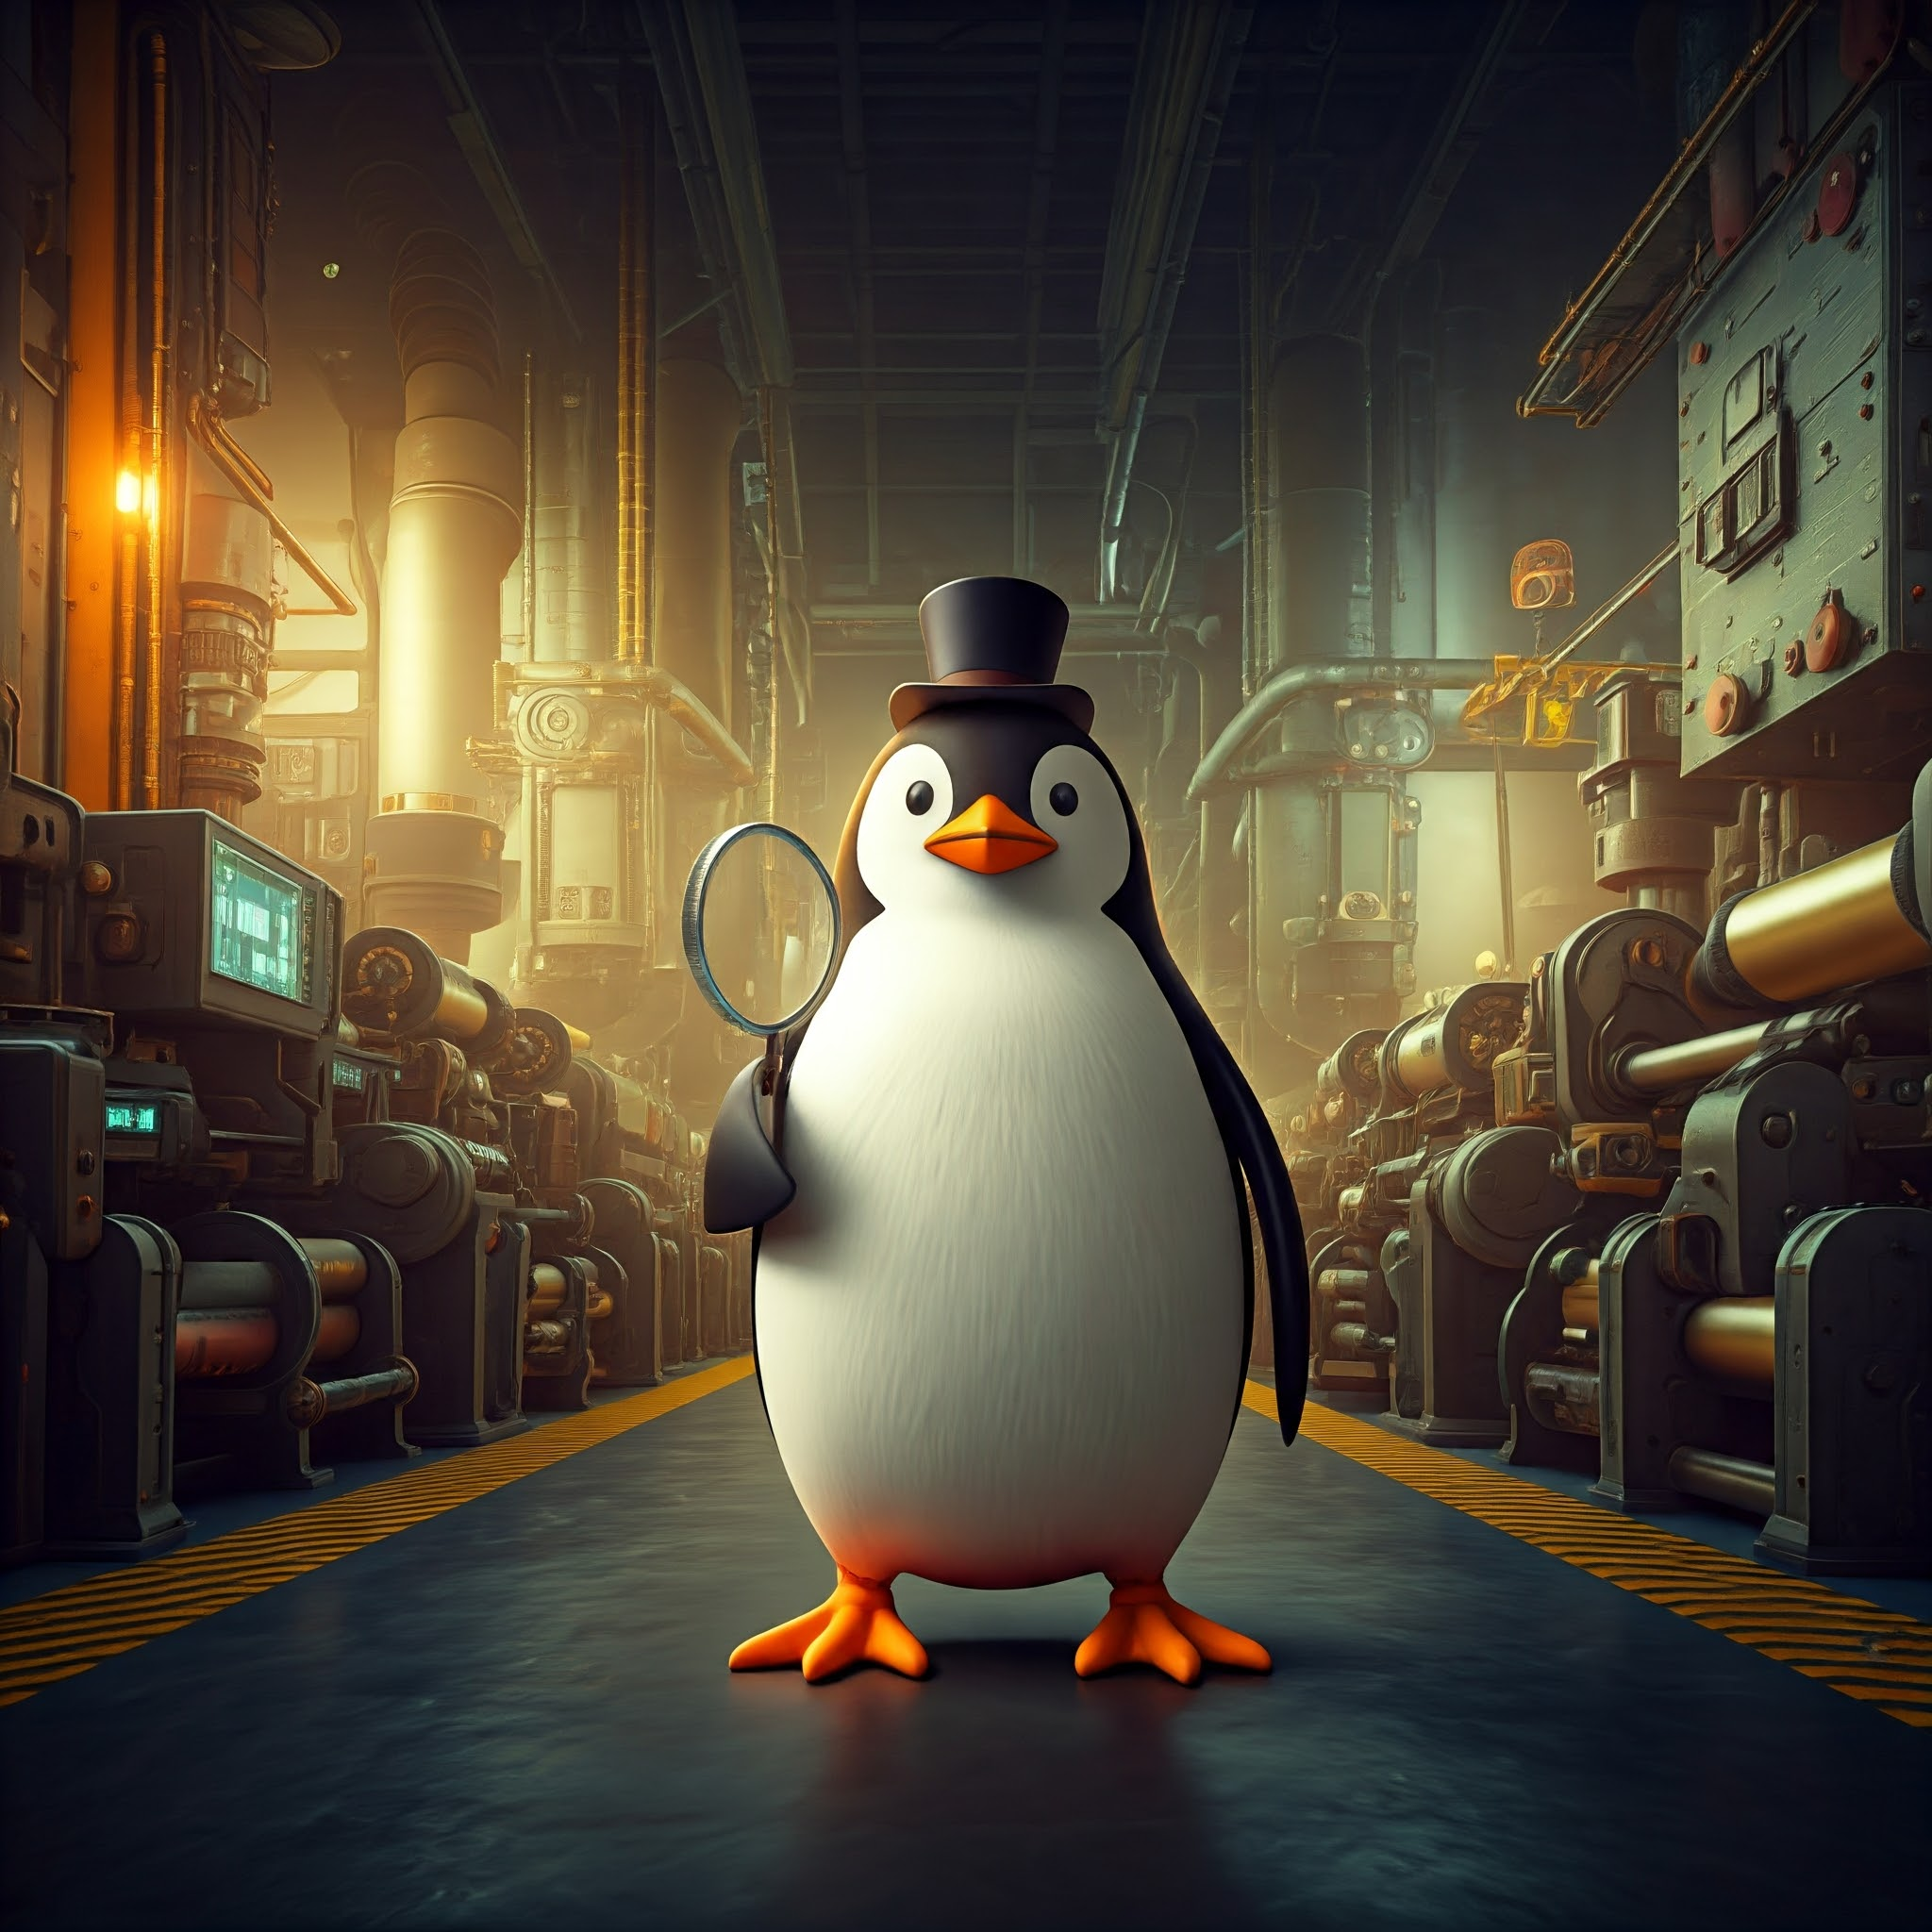
\includegraphics[width=1\textwidth ]{images/Copertina.jpeg}
    }
\end{figure}
\vfill 
\centering 
\includegraphics[width=0.4\textwidth ]{../../../preamble/Stemma_sapienza.png} \acc
\centering \Large \color{sapienza}Facoltà di Ingegneria dell'Informazione,
Informatica e Statistica\\
Dipartimento di Informatica
\end{titlepage}

%===================FINE COPERTINA======================%
\newpage
\pagecolor{cartaRiciclata}%\setmainfont{Algerian}
\Large
Questo documento è distribuito sotto la licenza 
\color{blue}\href{https://www.gnu.org/licenses/fdl-1.3.txt}{GNU}\color{black},  
è un resoconto degli appunti (eventualmente integrati con libri di testo) tratti dalle lezioni del corso di \jobname
\hphantom{a}per la laurea 
triennale in Informatica. Se dovessi notare errori, ti prego di segnalarmeli.\acc 
Nota bene : Essendo questi appunti di un corso esterno alla facoltà di Informatica, 
è presente un capitolo "Complementi" che può risultare utile al lettore.
\vfill
\begin{figure}[h!]
    \raggedright
    
\includegraphics[width=0.4\textwidth,right ]{../../../preamble/tomodachi.pdf} 
\end{figure}
\newpage %\setmainfont{Times New Roman}
\normalsize
\tableofcontents 
\newpage

%==================FOOTER e HEADER=======================%
\fancyhf{}
\fancyhead[L]{\nouppercase{\leftmark}}
\fancyhead[R]{Sezione \thesection}
\fancyfoot[C]{\thepage}
\fancyfoot[L]{Appunti di \jobname}
\fancyfoot[R]{ Marco Casu}
%\fancyfoot[R]{\setmainfont{Palace Script MT}\huge Marco Casu \setmainfont{Times New Roman}}
%==================FOOTER e HEADER=======================%

%Ricorda del comando \flowerLine per separare le sottosezioni. Le sezioni si separano nelle diverse pagine

%==================INIZIO======================%
\chapter{L'Automazione Industriale}
\section{Introduzione}
Con il termine \textit{Automazione}, si intende la trasformazione 
di un processo pre-esistente, al fine di renderlo autonomo, riducendo o 
sostituendo del tutto l'intervento umano, verrà trattata l'automazione 
dei processi industriali e manifatturieri, e del loro controllo e 
supervisione. I sistemi presi in considerazione evolvono nel 
tempo e reagiscono ad eventi, che ne cambiano lo stato, e scaturiscono 
dei feedback, per un eventuale correzione dell'errore.\acc 
Con sistema \textit{autonomo} si intende un sistema in cui viene 
ridotto l'intervento umano. L'\textit{Automatica} si occupa di 
sfruttare gli strumenti dell'informatica per l'automazione, acquisendo informazioni 
dal mondo fisico tramite appositi sensori, per poi essere elaborate 
su un sistema di controllo (calcolatore), o una rete di calcolatori, 
che implementa dei protocolli standard per l'industria. Differentemente da 
altri contesti, come la trasmissione (ad esempio, di un video in streaming) nelle 
reti dell'automazione i ritardi risultano critici, e vanno ridotti al 
minimo.
\begin{center}
    \begin{figure}[h!]
        \centering
        \includegraphics[width=0.4\textwidth ]{images/CIM.eps}
        \caption{Piramide CIM}
        \label{fig:cim}
   \end{figure}
   \end{center}
La \textit{piramide CIM}, mostrata in figura \ref{fig:cim}
schematizza la gestione di un processo industriale e delle sue procedure, 
ogni strato comunica con quelli adiacenti scambiandosi informazioni, nei 
livelli più alti, le informazioni sono più \textit{raffinate} ed 
astratte, nei livelli più bassi sono più grezze, ad esempio\begin{itemize}
    \item Al livello azienda viene decisa la produzione di un articolo (che 
    coinvolgerà l'utilizzo di un braccio robotico)
    \item Al livello macchina, l'informazione che arriverà al braccio 
    sarà semplicemente relativa ai gradi in cui i suoi giunti devono 
    ruotare
    \item Al livello di campo, l'informazione comprenderà semplicemente 
    il voltaggio da applicare alla macchina in questione per avere l'effetto 
    desiderato.
\end{itemize}
Con \textbf{cella}, si intende un unità composta da più macchine, in 
cui viene scambiato e lavorato del materiale per compiere delle azioni,
il \textit{controllo delle procedure} si occupa delle \textbf{macchine}, ed uno 
\textbf{stabilimento} è un complesso di celle/parti e catene 
di montaggio. nel livello di campo, vengono utilizzati vari dispositivi, 
quali\begin{itemize}
    \item motori elettrici, servomotori, encoder 
    \item azionatori di valvole, dinamo tachimetriche, sensori di temperatura
\end{itemize}
Tali sensori presenteranno un comportamento lineare, ad esempio, 
se una tensione $x$ causa una rotazione di $y$ giri per minuto, allora 
una tensione $2x$ causerà una  rotazione di $2y$. Anche se tali dispositivi 
non si prestano ad un comportamento lineare, ne verrà causata una volontaria 
linearizzazione, correggendone il comportamento.\acc 
Argomento centrale saranno i regolatori \textit{PID}, la cui definizione, 
come molte altre trattate in questo capitolo, sarà ripresa ed 
approfondita in seguito. tali regolatori agiscono su delle grandezze 
di campo.\begin{center}
    \begin{figure}[h!]
        \centering
        \includegraphics[width=1\textwidth ]{images/schemaPID.eps}
        \caption{schematizzazione del regolatore PID}
        \label{fig:schemaPID}
   \end{figure}
\end{center}
Si consideri il seguente esempio di regolatore, vi è una stufa che deve 
riscaldare una stanza, ed un sensore che ne misura la temperatura, il valore 
da raggiungere, detto \textit{setpoint}, è di 20 gradi celsius. Si supponga che il 
sensore, una volta rilevata la temperatura, debba accendere e spegnere la stufa 
in modo che si raggiunga la temperatura adeguata.
\begin{center}
    \begin{figure}[h!]
        \centering
        \includegraphics[width=0.6\textwidth ]{images/stufaEsempio.eps}
        \caption{Azioni sulla stufa}
        \label{fig:stufa}
   \end{figure} 
\end{center}
In figura \ref{fig:stufa}, il differenziale rappresenta un margine 
di differenza rispetto il setpoint, quando la temperatura è 
sotto il limite inferiore, la stufa viene accesa, quando è oltre il limite 
superiore, viene spenta (è chiaro che la velocità con la quale la temperatura 
cambia dipende dalle capacità della stufa e dalla dispersione del calore nella stanza).\acc 
Ridurre il valore del differenziale costringerebbe la temperatura ad assestarsi 
sempre di più sul valore desiderato, ma ciò, comporterebbe un'accensione/spegnimento della 
stufa più frequente, aumentando lo \textit{sforzo di controllo}, è quindi, in questo 
caso, accettabile un differenziale di $2^\circ$.\acc 
Tale modello di controllo è il più semplice che ci sia, esistono ovviamente altri modi di regolare un 
segnale in modo che esso raggiunga il valore desiderato, ad esempio, calcolare l'errore $e$ (ossia la differenza 
fra il valore desiderato ed il valore effettivo) e scalarlo ad una certa costante $K_p$ per poi utilizzare tale 
valore nella regolazione del segnale.
\begin{center}
    \begin{figure}[h!]
        \centering
        \includegraphics[width=0.6\textwidth ]{images/stufaEsempioPROP.eps}
        \caption{Regolatore proporzionale}
        \label{fig:regPropStuda}
   \end{figure} 
\end{center}
Anche se la variazione della temperatura è continua nel tempo, il suo 
superare una certa soglia è un evento, i PLC (controllori logici programmabili) 
agiscono sulle misure di campo, un noto linguaggio utilizzato per descriverne 
il funzionamento è noto come \textit{Sequential Flow Chart (SFC)}.\acc 
Nei sistemi di automazione industriale vengono prediletti controllori e sensori distribuiti piuttosto 
che centralizzati, se ne vuole dare una dimostrazione pratica con il seguente 
esempio : Siano dati i due modi per trasportare un oggetto 
su un nastro trasportatore\begin{center}
    \begin{figure}[h!]
        \centering
        \includegraphics[width=0.6\textwidth ]{images/rulli.eps}
        \caption{Rulli}
        \label{fig:rulli}
   \end{figure} 
\end{center}
Ogni nastro ha un sensore, se un oggetto è rilevato sopra il nastro, allora il motore si attiva. Risulta più efficiente 
la soluzione con 3 nastri in quanto sarà adoperata solamente la zona del nastro in cui è rilevato l'oggetto, piuttosto 
che l'intero nastro.\acc 
Per la modellizzazione di sistemi autonomi verranno adoperati automi a stati finiti, ampiamente trattati nel 
corso di 
\color{blue}\href{https://github.com/CasuFrost/University_notes/blob/main/Terzo%20Anno/Automi%2C%20Calcolabilit%C3%A0%20e%20Complessit%C3%A0/Automi%2C%20Calcolabilit%C3%A0%20e%20Complessit%C3%A0.pdf}{Automi, Calcolabilità e Complessità}
\color{black}, e \textit{Reti di Petri}. Una rete di Petri, non è altro che un grafo bipartito, in cui ogni nodo 
appartiene ad un'insieme fra \begin{itemize}
    \item nodi \textit{posto}
    \item nodi \textit{transizione}
\end{itemize}
Inoltre, i nodi posto possono essere annotati con dei pallini neri, detti \textit{token}, essi rappresentano 
lo stato del sistema in quanto indicano che delle risorse (in senso generale) sono disponibili in un posto, 
permettendo eventualmente una transizione. Ogni arco del grafo collega un nodo posto ad un nodo transizione.
\begin{figure}[h!]
    \centering
    \begin{tikzpicture}
        \node[place,tokens=2,label=above:$p_1$]        (p1) {};
        \node[place,label=above:$p_2$,right=of p1] (p2) {};
        \node[place,tokens=1,label=above:$p_3$,right=of p2] (p3) {};
        \node[place,label=above:$p_4$,below=of p3,right=of p3] (p4) {};
        \node[place,tokens=1,label=above:$p_5$,below=of p1] (p5) {};
       
      
        \node[transition,below right=of p1,label=below:$t_1$] {}
          edge[pre]                 (p1)
          edge[post] node[auto] {} (p2)
          edge[post] node[auto] {} (p5);
        \node[transition,below right=of p2,label=below:$t_2$] {}
          edge[pre]                 (p2)
          edge[post] node[auto] {} (p3)
          edge[post] node[auto] {} (p4);
      \end{tikzpicture}
      \caption{Esempio di una rete di Petri}
\end{figure}\acc
Le macchine per l'automazione possono essere di vari tipi, ad esempio, comprendere un unico attuatore, e più 
meccanismi di attuazione del moto che utilizzano una sola fonte. Un altro tipo di macchine sono quelle 
a \textit{controllo numerico}, macchine programmate per fare compiti elementari periodicamente. \acc 
Quando in un processo produttivo il materiale viene trasformato in maniera continuativa (come nell'industria 
farmaceutica o alimentare) si parla di \textbf{produzione continua}. Nel caso in cui i materiali sono processati 
in quantità finite e determinate si parla di \textbf{produzione a lotti}, le pause fra la lavorazione di un lotto 
e l'altro sono dovute al fatto 
che è necessario trasformare solo una determinata quantità di materiale grezzo.\acc 
L'automazione industriale fa largo utilizzo dei \textit{robot}, bracci meccanici che presentano diversi 
gradi di libertà, ossia giunti, che possono ruotare attorno un certo asse. 
   \begin{center}
	\begin{tabular}{>{\centering\arraybackslash}m{3in}>{\arraybackslash}m{3in}}
        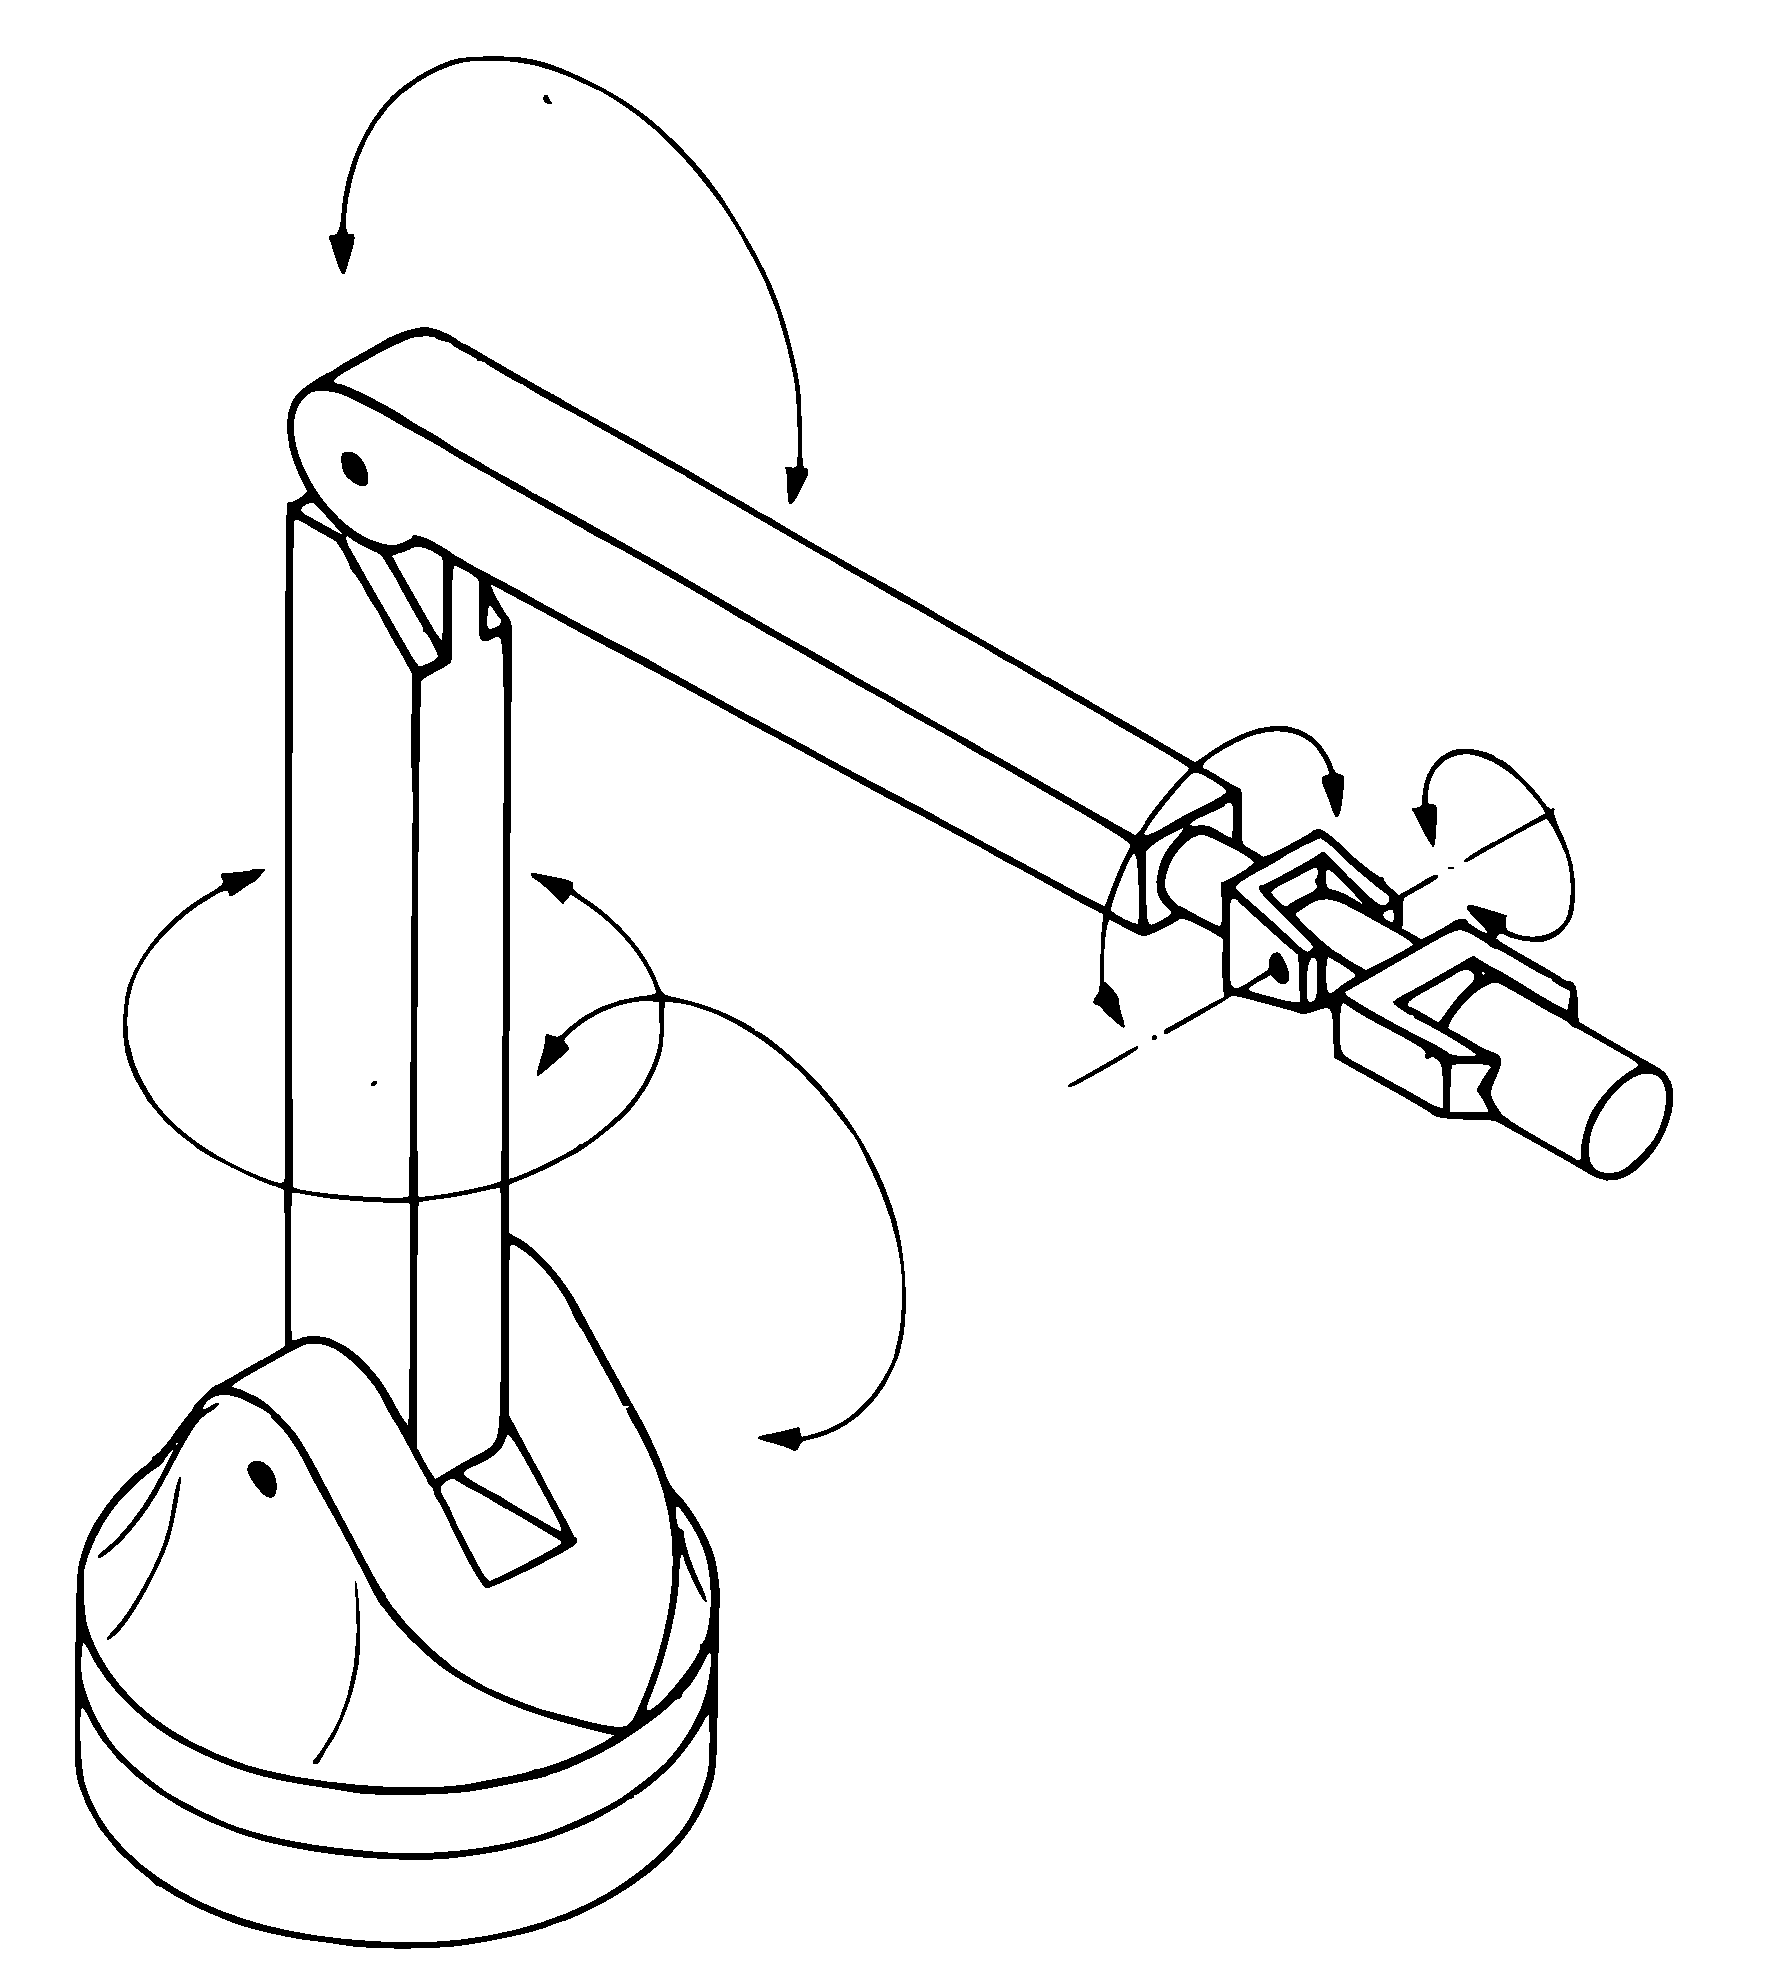
\includegraphics[width=0.3\textwidth ]{images/braccioRobot.pdf} & L'organo terminale, posto alla fine 
        del braccio (in un certo senso, la sua "mano"), può assumere una certa configurazione (posizione e direzione) a 
        seconda della rotazione di ogni giunto del braccio. 
        Si può dire che la posizione finale $p$ e la sua direzione sono in funzione degli angoli 
        $\theta_1,\theta_2\dots,\theta_n$ di rotazione di ogni giunto.
		\\
	\end{tabular}
\end{center}
La procedura di comando da far eseguire al robot si traduce in una funzione nel tempo che descrive in che modo 
deve variare la rotazione di ogni singolo giunto, quest'ultima al livello di campo, si traduce nell'attuazione 
dei motori elettrici posti sui giunti.
\begin{center}
        \includegraphics[width=1\textwidth ]{images/rotBraccioRobot.eps}
\end{center}
Altri tipi di macchine per la movimentazione oltre i robot sono i rulli o i carrelli automatici, questi ultimi 
inizialmente potevano muoversi seguendo un percorso stabilito da magneti posti sul terreno, vengono dotati di 
sensori di prossimità per evitare collisioni. I carrelli moderni non sono limitati da percorsi prestabiliti, sono 
autonomi e possono fare percorsi arbitrari, che vengono calcolati da un elaboratore che ha la "visione" completa 
di essi.\acc 
Sorge spontaneo chiedersi quale sia la differenza fra Automazione e Robotica.\begin{itemize}
    \item \textit{Analogie} : Entrambe coinvolgono l'informatica ed i calcolatori, interfacciandosi con il mondo 
    fisico, entrambe sfruttano conoscenze e tecnologie multi-disciplinari. 
    \item \textit{Differenze} : La robotica mostra la fattibilità di una soluzione, l'automazione si occupa di 
    porsi delle domande riguardo tale soluzione, fra cui l'efficienza, l'ottimalità e l'affidabilità.
\end{itemize}
Formalmente, si definisce \textbf{processo} la \textit{trasformazione} di \textit{materiali} in 
\textit{prodotti}. Tale trasformazione richiede 
\begin{itemize}
    \item Energia 
    \item Informazione 
    \item Controllo
\end{itemize}
Anche la costruzione di uno strumento per la caccia da parte di un uomo primitivo è un processo, in quel caso, 
l'energia è data dai muscoli del corpo, l'informazione viene dai sensi, quali vista e tatto, ed il controllo 
avviene da parte del cervello.
\begin{center}
    \includegraphics[width=0.5\textwidth ]{images/caveMan.eps}
\end{center}
Lo scopo dell'automazione nel tempo è stato quello di sostituire o eliminare l'intervento dell'uomo 
nei processi, spesso è faticoso e pericoloso fornire energia, e l'uomo non ha le capacità sufficienti per 
gestire in maniera precisa l'informazione ed il controllo.\acc 
Il \textbf{primo passo} di industrializzazione è stato quello di sostituire l'energia fornita dall'uomo con l'energia 
naturale ed animale, durante la prima rivoluzione industriale, dove la produzione dipendeva da macchine 
azionate tramite potenza meccanica derivante da fonti energetiche come mulini.\acc 
Il \textbf{secondo passo} riguarda la sostituzione delle operazioni di controllo, un importante esempio fu il 
\textit{regolatore di velocità} di Watt (1785), fu la prima applicazione di regolatore automatico, e sfruttava 
la forza centrifuga di due masse in rotazione per regolare la velocità di una macchina a vapore.
\begin{figure}[h!]
    \centering
    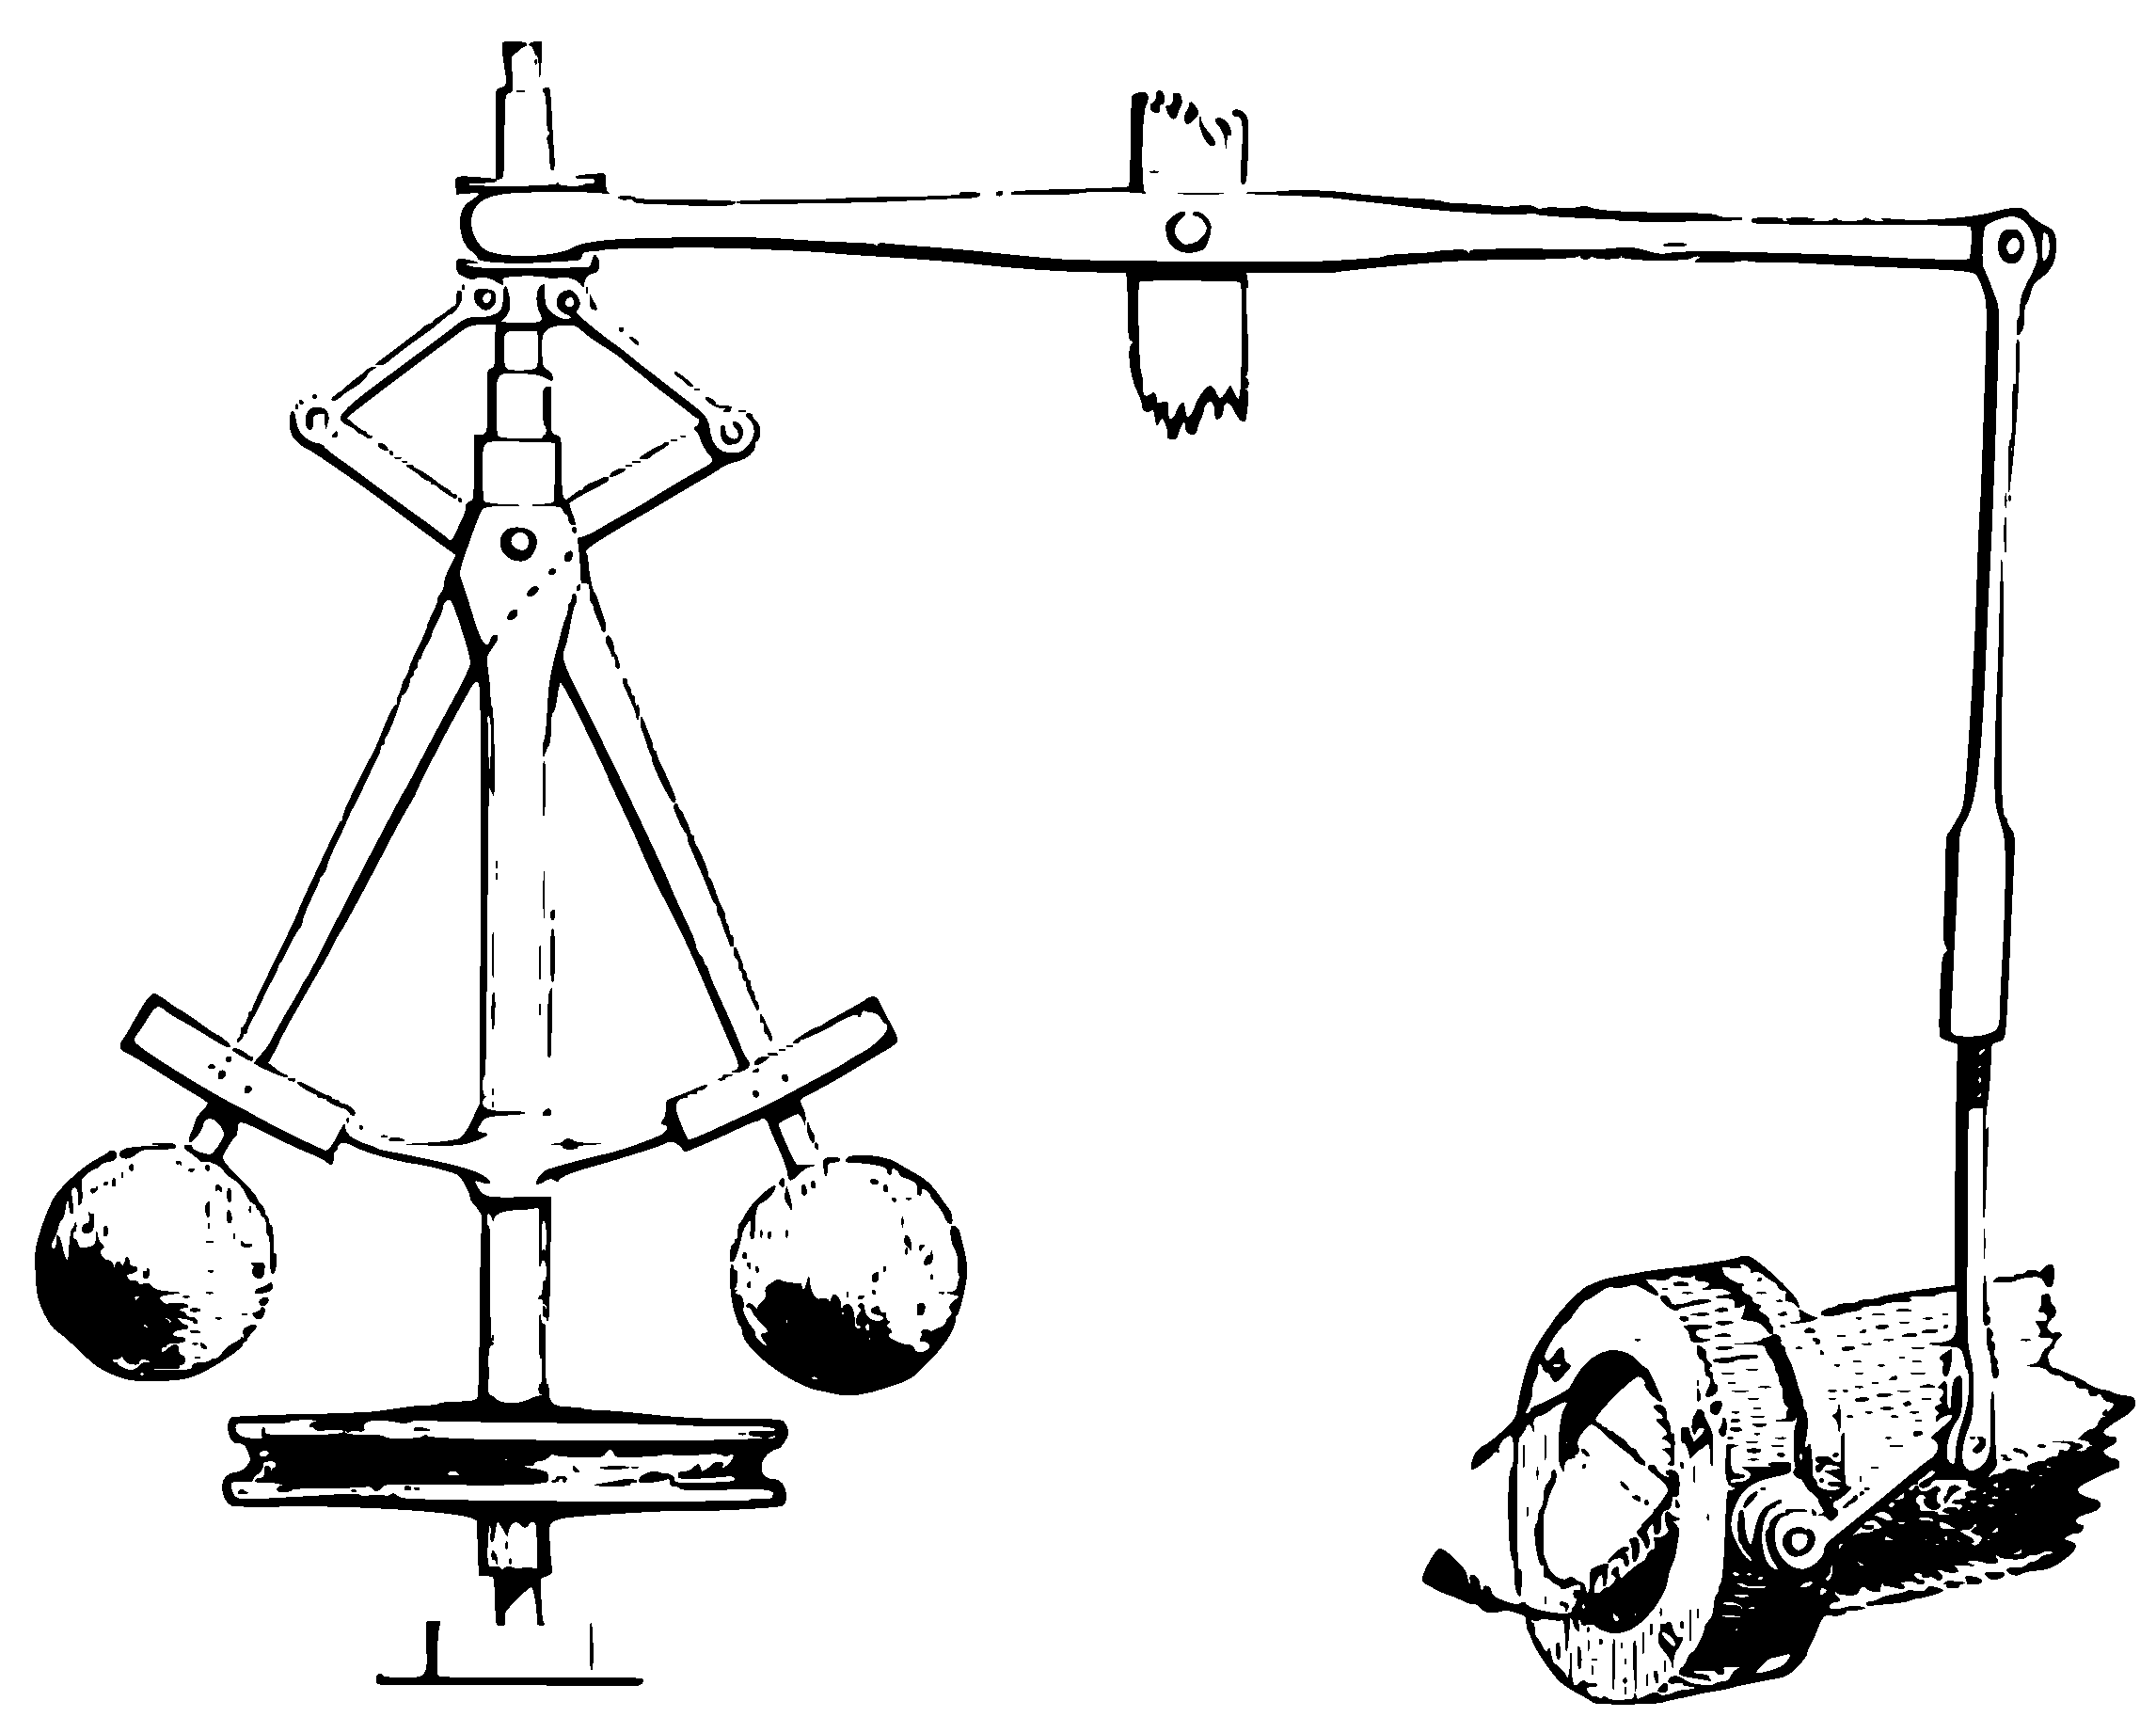
\includegraphics[width=0.4\textwidth ]{images/watt.pdf}
    \caption{regolatore di Watt}
    \label{fig:watt}
\end{figure} \acc
Il funzionamento è semplice, il vapore passante per la valvola fa aumentare la velocità di rotazione del 
regolatore, per la forza centrifuga, le masse poste sulla valvola a farfalla si allontanano, alzandosi, 
qui la gravità oppone resistenza facendo chiudere la valvola essendo che le masse tendono ad avvicinarsi al 
suolo, facendone diminuire la velocità di rotazione.  
Tali automatismi sono compresi dalla teoria dei controlli automatici, che definisce l'azione di comando più efficace 
per ottenere il comportamento desiderato a seguito di una certa misurazione fisica.\acc
Il \textbf{terzo passo} riguarda la gestione delle informazioni mediante sistemi combinatori/sequenziali che al 
verificarsi di determinate condizioni reagiscono con operazioni di base. La prima generazione di controllori 
prevedeva circuiti elettronici composti da bobine e relé, essi erano ingombranti e lenti nell'acquisizione 
delle informazioni, inoltre la loro logica era prestabilita e ridefinirla scaturiva una modifica sostanziale 
del circuito. \acc 
Con l'avvento dei semiconduttori si è introdotta la seconda generazione di controllori, basati su schede 
elettroniche stampate, riducendo i costi ed aumentando l'efficienza, non risolvendo però il problema della bassa 
flessibilità, in quanto tali schede erano progettate per gestire una specifica logica. \acc 
La terza generazione di controllori vede i microprocessori protagonisti, grazie all'evoluzione dell'elettronica 
e dell'informatica sono ad oggi utilizzabili schede riprogrammabili (PLC) altamente flessibili, capaci di eseguire 
un generico algoritmo logico sequenziale.
\begin{center}
    \begin{tabular}{|c|c|c|}
        \hline
        \rowcolor[HTML]{6665CD} 
        {\color[HTML]{FFFFFF} Rivoluzione Industriale} & {\color[HTML]{FFFFFF} Periodo Temporale} & {\color[HTML]{FFFFFF} Tecnologie e Caratteristiche}                                                                                                                                                                                                                                                                                                                               \\ \hline
        \rowcolor[HTML]{DAE8FC} 
        prima                                          & 1785 – metà 19° secolo                   & \begin{tabular}[c]{@{}c@{}}utilizzo di macchine azionate da energia\\  meccanica (vapore, acqua)\end{tabular}                                                                                                                                                                                                                                                                     \\ \hline
        \rowcolor[HTML]{F2F7FE} 
        seconda                                        & fine 19°secolo – 1970                    & \begin{tabular}[c]{@{}c@{}}azionamento elettrico delle macchine e produzione\\  di massa basata sulla\\  divisione del lavoro (catene di montaggio)\end{tabular}                                                                                                                                                                                                                  \\ \hline
        \rowcolor[HTML]{DAE8FC} 
        terza                                          & 1970 – oggi                              & \begin{tabular}[c]{@{}c@{}}utilizzo dell'elettronica e delle tecnologie\\  dell'informazione (IT) \\ per aumentare il livello di automazione di attività\\  complesse (CNC, robot e computer)\end{tabular}                                                                                                                                                                         \\ \hline
        \rowcolor[HTML]{F2F7FE} 
        quarta                                         & oggi – futuro                            & \begin{tabular}[c]{@{}c@{}}sviluppo di macchine sensorizzate e intelligenti,\\  interconnesse tra loro e con internet, con la raccolta,\\  analisi e uso di grandi \\ quantità di informazioni (Big data), per una\\  specializzazione di \\ massa del prodotto, l'integrazione della\\  catena produttiva \\ (supply and value chains) e una maggiore\\  efficienza\end{tabular} \\ \hline
        \end{tabular}
\end{center}
\flowerLine
\section{Processi Industriali}
I sistemi di produzione automatizzati sono composti da 
diverse componenti\begin{itemize}
    \item processo produttivo - movimentazioni meccaniche, attuazioni, 
    trasformazioni fisiche e chimiche 
    \item sistema di controllo - uno o più dispositivi messi in comunicazione 
    con il processo produttivo, che possono agire su di esso riducendo 
    l'intervento umano. 
    \item impianto di produzione - macchinari, edifici, componenti
\end{itemize}
Si considerino i seguenti esempi di produzione industriale\begin{itemize}
    \item \textbf{produzione di energia elettrica} \begin{itemize}
        \item materie prime (input continuo) : combustibile fossile, ossigeno 
        \item prodotto (output continuo) : energia elettrica misurata in Kilowatt/ore
        \item impianto necessario : tubature, caldaia, turbine, bruciatori, pompe, valvole, camini, edifici di
        sostegno e di contenimento, sensori
        
    \end{itemize}
    \item \textbf{produzione di vernice} \begin{itemize}
        \item materie prime (input continuo) : resine, coloranti, acqua, additivi
        \item prodotto (output discreto) : barattoli di vernice
        \item impianto necessario : reattori (dove avvengono le reazioni principali), miscelatori, riscaldatori,
        tubature, pompe, valvole, edificio di sostegno e di contenimento, sensori
    \end{itemize}
    \item \textbf{produzione di parti meccaniche di motori} \begin{itemize}
        \item materie prime (input discreto) : pezzo metallico grezzo
        \item prodotto (output discreto) : componente del motore
        \item impianto necessario : macchina con mandrini per la meccanica (fresatura, foratura, ...), sistema di
        controllo numerico (posizionamento corretto dell'utensile del mandrino),
        dispositivo di cambio utensile automatico, protezioni, sistemi di scarico
        trucioli
    \end{itemize}
\end{itemize}
\subsection{Sistema di Controllo}
Il sistema di controllo interagisce con il processo 
attraverso \textit{sensori} e \textit{trasduttori}. Acquisiscono 
informazioni dal mondo fisico (pressione, temperatura) e le convertono in segnali 
facilmente analizzabili e controllabili (segnali elettrici).
\acc 
Un esempio di sensore per misurare la forza, consiste in un circuito il cui
resistore viene deformato quando rilevata una pressione sul sensore, 
variandone la resistenza.\acc 
Una volta raccolte le informazioni, è possibile cambiare le variabili 
di controllo del processo per ottenere il comportamento desiderato. Solitamente, 
il segnale di controllo è a bassa potenza, non sufficiente per correggere il comportamento 
di grossi attuatori, a tal proposito sono adoperati gli \textit{amplificatori}. Le informazioni 
sono elaborate da un apposito calcolatore che può essere inglobato o 
esterno alla macchina in questione.\acc
Nei sistemi di controllo è stata definita una normativa, nota come 
IEC61499 per normalizzare il funzionamento generale di tali 
dispositivi. In particolare,  un sistema di controllo deve 
rifarsi ai seguenti punti\begin{itemize}
    \item è un sistema informatico che elabora informazioni ed 
    esegue/applica algoritmi.
    \item è costituito da vari dispositivi che comunicano attraverso un'apposita 
    rete. 
    \item i dispositivi devono implementare delle funzionalità, denominate \textit{applicazioni}.
    \item tali applicazioni possono essere distribuite fra i vari dispositivi. 
    \item i dispositivi devono interfacciarsi con la rete e con il processo, 
    inoltre le applicazioni costituiscono le loro \textit{risorse}.
    \item in generale, una \textit{risorsa} è costituita da\begin{itemize}
        \item una o più applicazioni 
        \item funzioni che collegano dati ed eventi 
        \item funzioni di pianificazione delle attività (un sistema operativo)
    \end{itemize}
\end{itemize}
\begin{figure}[h!]
    \centering
    \includegraphics[width=1\textwidth ]{images/sistemaControllo.eps}
    \caption{schematizzazione di un sistema di controllo}
    \label{fig:siscon}
\end{figure} 
Si definisce \textbf{Manufacturing} l'insieme dei processi 
produttivi da applicare per ottenere un prodotto finale desiderato, a partire 
da materiali grezzi. Richiede \begin{itemize}
    \item energia 
    \item macchine 
    \item intervento umano 
    \item informazioni
\end{itemize}
Da un punto di vista economico, è il processo che da valore aggiunto
ai materiali utilizzati.\begin{center}
    \includegraphics[width=0.7\textwidth ]{images/manifacturing.eps}
\end{center}
Spesso di questi processi produttivi ce ne sono molteplici messi a catena, in modo che l'output di un 
processo sia l'input di un altro. Si consideri il seguente esempio che schematizza un sistema di produzione del cemento.
\begin{figure}[h!]
    \centering
    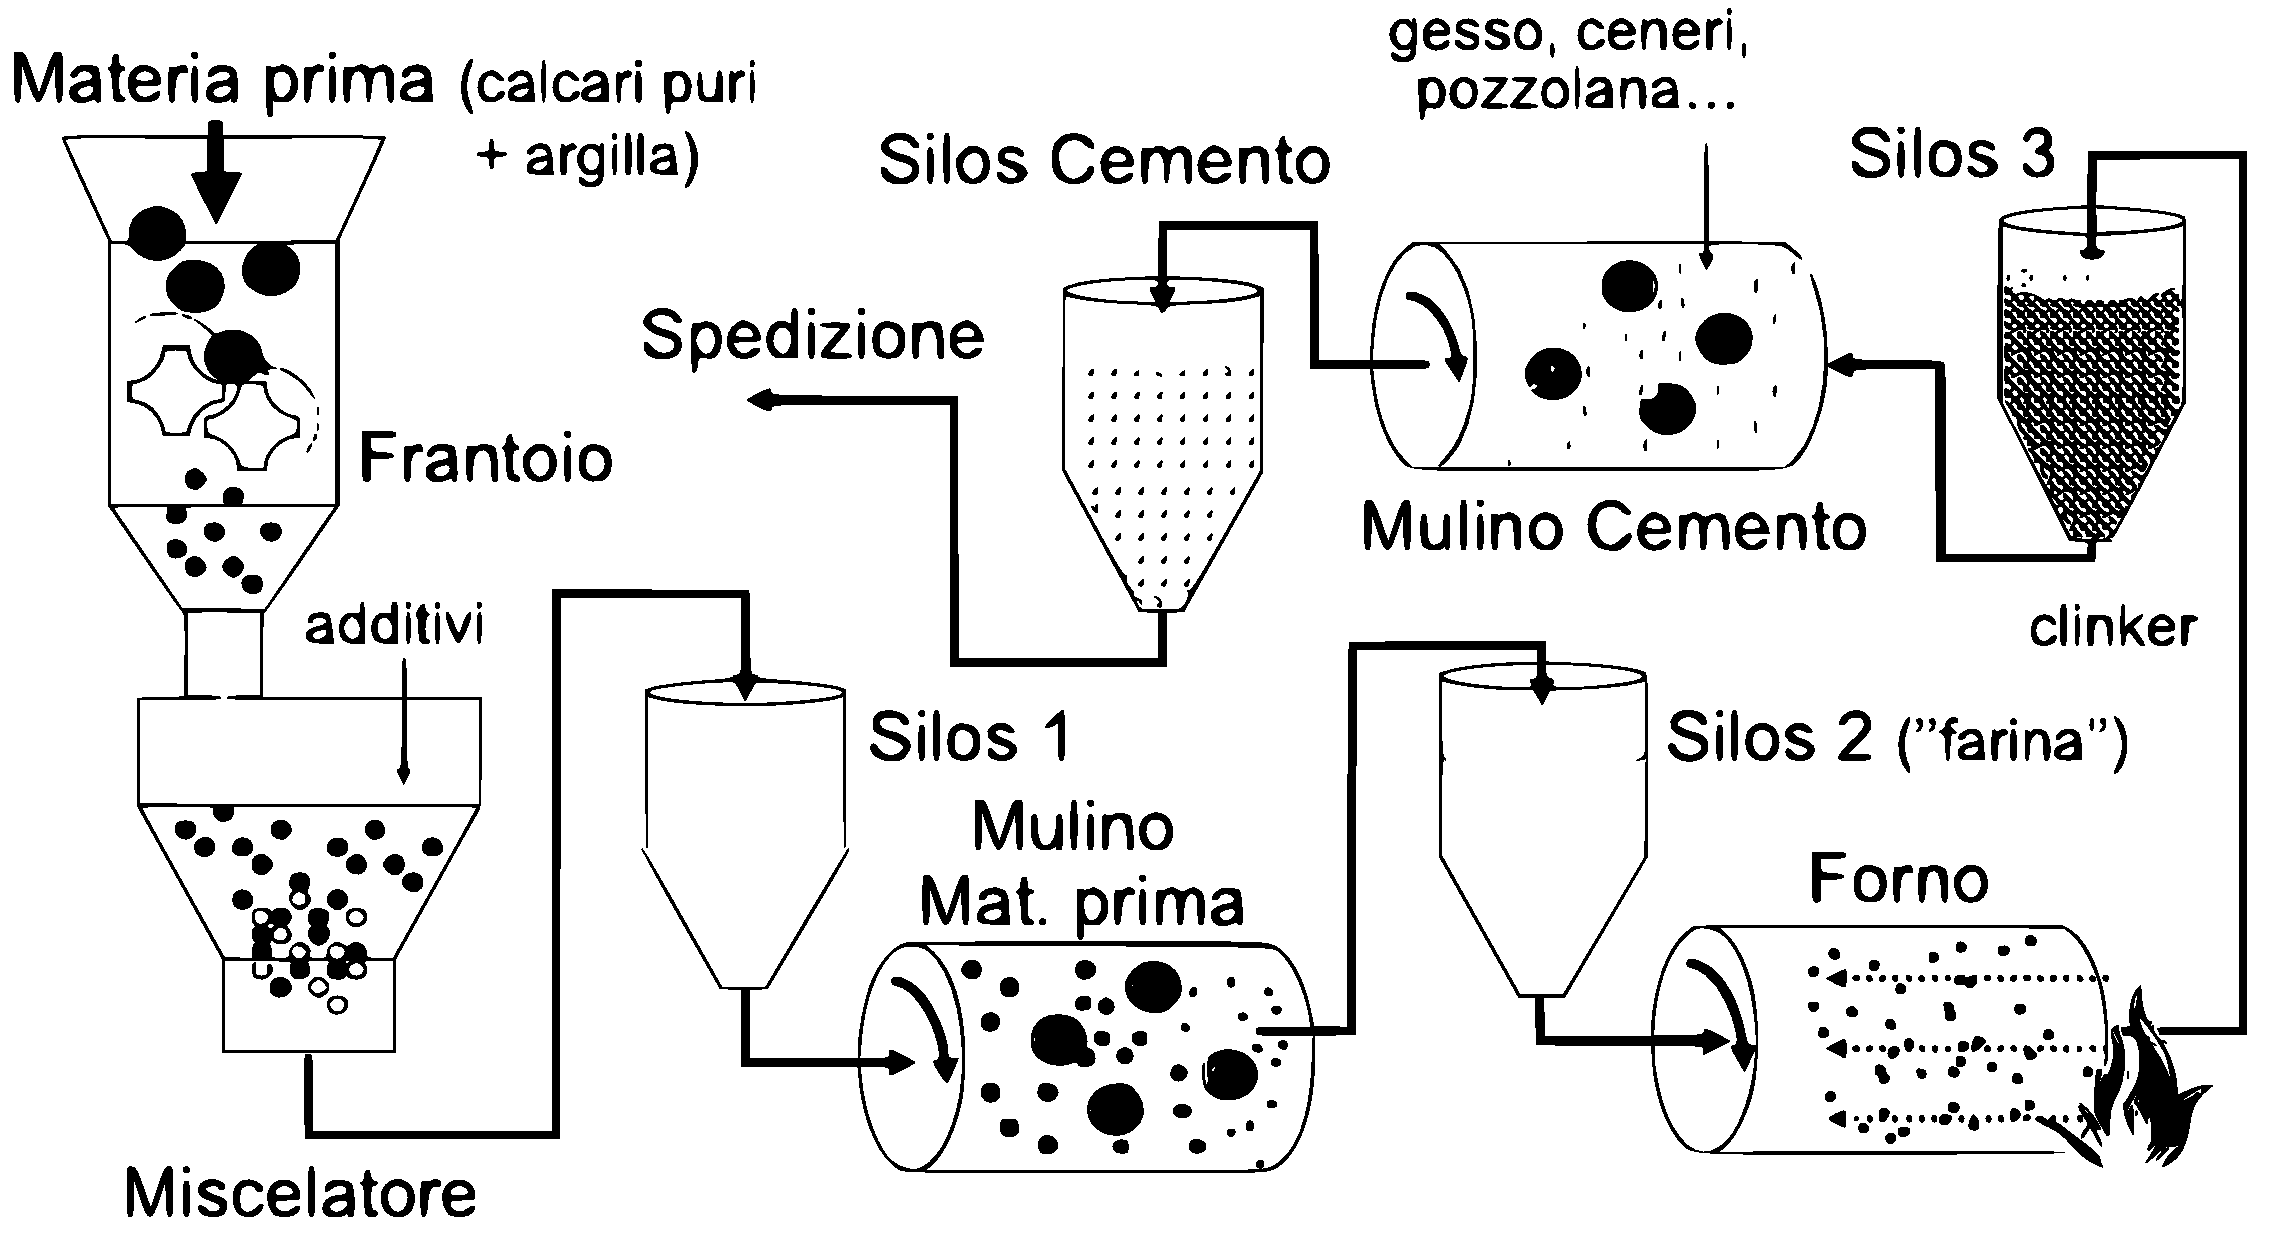
\includegraphics[width=0.7\textwidth ]{images/cementificio.pdf}
    \caption{Cementificio : schema}
    \label{fig:cementificio}
\end{figure} 
Il cemento viene prodotto a partire da calcari puri ed argilla, viene mandato nel frantoio per essere 
tritato, ciò che ne esce viene miscelato per poi venire accumulato in un silos. Quest'ultimo, funge 
da \textit{buffer}, ossia un accumulo del prodotto non ancora terminato durante la sequenza di produzione, utile 
nel sincronizzare la catena, qui 
viene riempito totalmente prima di passare allo step successivo. Il primo mulino esegue una fase 
di pre riscaldamento, il calore utilizzato deriva dall'energia termica scartata dal forno principale 
ad alte temperature. \acc 
Il processo consiste in una \textit{sequenza} di \textit{operazioni elementari} di varia natura \begin{itemize}
    \item lavorazione  e assemblaggio
    \item trasporto e stoccaggio 
    \item verifica, test, e coordinamento
\end{itemize}
Fin'ora è stata evidenziata la \textit{numerabilità} delle materie prime o del prodotto finale di un certo 
processo, a tal proposito, è possibile classificare i processi produttivi nel seguente 
modo
\begin{center}
    \includegraphics[width=0.7\textwidth ]{images/classificazioneProcProd.eps}
\end{center}
\begin{itemize}
    \item\textbf{processi continui} : Trattano la trasformazione continua nel tempo della materia, energia 
    e quantità di moto. L'obiettivo è mantenere uniforme nel tempo la qualità del prodotto, gli scambi 
    avvengono sulle variabili fisiche.
    \item\textbf{processi a lotti} : Possono essere sia continui che discreti, il lavorato finale necessita 
    di una specifica, e finita, quantità di materia prima per essere prodotto. Segue una determinata 
    sequenza di lavorazione detta \textit{ricetta}, il processo si intorrempe fra un lotto ed un 
    altro. Obbiettivo dell'automazione è la definizione delle ricette, garantire un uso corretto delle 
    risorse e realizzare tali sistemi in modo che siano ripetibili.
    \item\textbf{processi semi continui} : La produzione avviene in lotti o batch, con fasi di lavorazione continue intervallate da pause per il cambio di prodotto o la pulizia dell'impianto
    \item \textbf{processi discreti} : Si lavora su singoli prodotti, materiali numerabili, è una 
    produzione tipica dell'industria manifatturiera.
\end{itemize}
I sistemi di controllo dei processi prevedono azioni di tipo \textit{logico} oppure \textit{diretto}\begin{center}
    \begin{tabular}{
        >{\columncolor[HTML]{ECF4FF}}c |
        >{\columncolor[HTML]{FFFFFF}}c |
        >{\columncolor[HTML]{FFFFFF}}c |}
        \cline{2-3}
        \cellcolor[HTML]{FFFFFF}                                        & \cellcolor[HTML]{ECF4FF}Controllo logico                                                                                                                                    & \cellcolor[HTML]{ECF4FF}Controllo diretto                                                                                                                                           \\ \hline
        \multicolumn{1}{|c|}{\cellcolor[HTML]{ECF4FF}Processi continui} & \begin{tabular}[c]{@{}c@{}}coordinamento complessivo\\  avviamento\\  e spegnimento guasti e emergenze\end{tabular}                                                         & \begin{tabular}[c]{@{}c@{}}controlli primari \\ (livelli, temperature, pressioni)\\  controlli asserviti (portata pompe, \\ posizione valvole)\end{tabular}                         \\ \hline
        \multicolumn{1}{|c|}{\cellcolor[HTML]{ECF4FF}Processi a lotti}  & \begin{tabular}[c]{@{}c@{}}controllo delle ricette\\  supervisione impianto\\  avviamento e  spegnimento guasti\\  e emergenze \\ allocazione risorse impianto\end{tabular} & \cellcolor[HTML]{FFFFFF}\begin{tabular}[c]{@{}c@{}}controlli primari (livelli,\\  temperature, pressioni)\\  controlli asserviti (portata pompe, \\ posizione valvole)\end{tabular} \\ \hline
        \multicolumn{1}{|c|}{\cellcolor[HTML]{ECF4FF}Processi discreti} & \begin{tabular}[c]{@{}c@{}}controllo sequenze di lavoro \\ delle singole macchine \\ supervisione impianto \\ avviamento e spegnimento \\ guasti e emergenze\end{tabular}   & \begin{tabular}[c]{@{}c@{}}controlli asserviti (posizionamento,\\  velocità \\ motori elettrici)\end{tabular}                                                                       \\ \hline
        \end{tabular}
\end{center}
\begin{itemize}
    \item \textit{regolazione} : Portare un segnale ad un determinato valore di riferimento 
    \item \textit{asservimento} : Far si che il segnale segua una certa dinamica nel tempo
\end{itemize}
Il \textit{controllo diretto} riguarda il rilevamento di grandezze fisiche analogiche da parte di 
sensori posti sul campo, tali valori continui nel tempo vengono 
convertiti in segnali digitali, confrontandoli poi con il valore di riferimento, dando l'azione di comando 
per correggere il comportamento delle variabili.\begin{enumerate}
    \item I sensori forniscono un segnale \textbf{analogico} $x(t)$ continuo nel tempo (temperatura, posizione)
    \item Tale segnale viene \textbf{quantizzato}, denotato $x_q(t)$, costringendolo ad assumere un numero limitato di 
    valori prestabiliti $\Delta$, separati da un ampiezza $q$, il numero di bit necessari 
    a rappresentare i valori del segnale sarà $n=\log_{2}(\nicefrac{\Delta}{q})$
    $$ x_q(t)=\lfloor\frac{x(t)}{q}\rfloor\cdot q$$
    \item Il segnale analogico quantizzato viene poi \textbf{campionato}, ossia, viene valutato 
    esclusivamente in determinati intervalli di tempo separati da un tempo di campionamento $T_C$ 
    $$x_q(t) \longrightarrow  x_q(kT_C)\ \ \ \ t\in\R \ \ k\in\mathbb{Z}$$
    \item A tal punto si ha un \textbf{segnale digitale} codificato in numeri binari che può essere 
    elaborato su un sistema di controllo digitale.
\end{enumerate}
\begin{center}
    \includegraphics[width=1\textwidth ]{images/segnale.eps}
\end{center}
Le variabili logiche, ad esempio quelle booleane, assumono valori in un insieme numerabile, e su di esse 
è possibile eseguire operazioni logiche, si consideri il seguente esempio : \begin{quote}
    \color{gray}
    Il comando $M$ è una variabile booleana che, se vera, aziona il moto di un motore elettrico. 
    Il sensore di prossimità è descritto da una variabile booleana $P$ che è vera se ci sono 
    ostacoli nelle vicinanze, la variabile $C$ descrive il consenso nel voler attivare il motore.\acc 
    Risulta chiaro che $$ M= C \land \lnot P$$\color{black}
\end{quote}
Il seguente SFC (Sequential Functional Chart) descrive il comportamento logico di una timbratrice 
automatica.\begin{center}
    \includegraphics[width=0.7\textwidth ]{images/timbratrice.eps}
\end{center}
\flowerLine 
\section{Analisi dei Sistemi di Produzione}
Si considerino i sistemi di produzione manifatturiera, quindi, discreti. Essi possono seguire diverse strutture, 
fra le più importanti vi sono\begin{itemize}
    \item \textbf{linea di trasferta } : La produzione avviene secondo una specifica sequenza, rigida e non 
    flessibile. Un esempio tipico è la classica catena di montaggio introdotta da Ford. 
    \item \textbf{flow shop} : Vi sono diversi macchinari, e più flussi di produzione che si 
    alternano i macchinari diversi. 
    \item \textbf{job shop} : Ci sono differenti percorsi, intrecciati e complessi fra i diversi macchinari 
    e reparti dell'impianto di produzione. 
    \item  \textbf{celle di produzione} : Le singole celle contengono più macchinari, ed ognuna di queste 
    si occupa della produzione (dall'inizio alla fine) di un singolo prodotto, mantenendola concentrata 
    nella cella, senza che essa sia dislocata nell'impianto. 
    \item \textbf{FMS} : Diversi flussi fra le varie celle.
\end{itemize}
Vanno considerati vari aspetti nell'analisi dei sistemi di produzione, come la trattazione dei tempi di 
attesa, il \textit{WIP - work in process}, è un termine utilizzato per indicare il numero di pezzi che vengono 
lavorati contemporaneamente.
\begin{figure}[h!]
    \centering
    \includegraphics[width=0.8\textwidth ]{images/lineaFlowJob.eps}
    \caption{sistemi di produzione}
    \label{fig:sisprod}
\end{figure} 
\subsection{Linee di Trasferta}
Verrà trattata in questa sezione la modellizzazione delle linee di trasferta, e verranno analizzati 
alcuni parametri che le caratterizzano. Una linea di trasferta consiste in una serie di macchine o stazioni 
(macchinari adatti a più compiti) connessi sequenzialmente da un sistema di trasporto. La sequenza di produzione 
è rigida ed i pezzi vengono processati continuamente nel tempo senza interruzioni. Le linee possono essere 
sincrone (i pezzi avanzano alla stessa velocità) oppure asincrone, tramite l'installazione di appositi 
buffer fra una macchina e l'altra.\begin{itemize}
    \item \textit{pro} : La produzione avviene per un singolo prodotto, risulta molto efficiente, il WIP è 
    ridotto ed il trasporto dei pezzi è semplice, dato che segue un unica direzione. I tempi di avvio sono brevi. 
    \item \textit{contro} : La produzione è poco flessibile ed è a rischio obsolescenza, il malfunzionamento 
    di una macchina può causare l'interruzione dell'intera linea (single point of failure).
\end{itemize}
\teo{(Legge di Little)} Data una linea di trasferta, ed i seguenti parametri \begin{itemize}
    \item $p$ : tasso di produzione misurato in pezzi per unità di tempo 
    \item $T_a$ : tempo necessario per l'attraversamento di una linea 
    \item $WIP$ il work in process,  il numero di pezzi che vengono 
    lavorati contemporaneamente
\end{itemize}
Vale la seguente relazione $$ WIP = p\cdot T_a$$
La legge si riferisce ad un sistema a regime permanente, quindi non considera l'avvio della linea, dato quindi 
un tasso $p$ fisso, per ridurre il $WIP$ è necessario ridurre il  tempo necessario 
per l'attraversamento della linea. 
\subsubsection{Esempio}
Verrà considerata una linea di trasferta composta da 3 macchine $M_1,M_2$ e $M_3$, i cui tempi di 
lavoro sono uguali e costanti $T_1=T_2=T_3=2$. Tale analisi è fatta a $WIP$ costante.
\begin{center}
    \includegraphics[width=0.5\textwidth ]{images/WIP1.eps}
\end{center}
In questo contesto, il WIP è 1, ciò significa che solamente un pezzo (indicato con una pallina verde) può 
occupare le 3 macchine contemporaneamente. Ogni 2 unità di tempo, il pezzo viene processato da una 
macchina all'altra, ci vogliono 6 unità di tempo per produrre un pezzo, $T_a=6$. 
$$T_a=6 \land WIP = 1 \implies p = \frac{1}{6} \text{ un pezzo ogni 6 unità di tempo}$$
\begin{center}
    \includegraphics[width=0.9\textwidth ]{images/WIP2.eps}
\end{center}
Si noti come nonostante il WIP aumenti, nel caso $WIP=4$ il tasso di produzione rimane invariato, 
risulta quindi fondamentale trovare il valore di WIP ottimale che minimizzi $T_a$ e 
massimizzi $p$. 
\begin{center}
    \begin{figure}[h!]
        \centering
        \includegraphics[width=0.9\textwidth ]{images/WIP3.eps}
        \caption{$ T_1 = 1\ \ \ \ \ T_2 = 2 \ \ \ \ \ T_3 = 3$}
        \label{fig:wip3}
    \end{figure}
\end{center}
L'esempio proposto in figura \ref{fig:wip3} è simile a quello precedente, ma in questo caso le macchine hanno tempi 
di lavoro differenti, precisamente, aumentano in ordine crescente. 
\begin{center}
    \begin{figure}[h!]
        \centering
        \includegraphics[width=0.9\textwidth ]{images/analisiWIP.eps}
        \caption{Analisi in funzione del $WIP$}
        \label{fig:wipAnalysis}
    \end{figure}
\end{center}
Con \textbf{Dimensionamento} e \textbf{Bilanciamento} di una linea di trasferta, si intende la ricerca del 
compromesso ideale fra l'aumento della produttività (utilizzo di più macchine) e la riduzione dei costi, 
a parità di tempo totale di lavorazione. Le curve in figura \ref{fig:carico}, descrivono l'allocazione delle 
lavorazioni (distribuzione del carico) in un numero fissato di $N$ stazioni/macchine.
\begin{figure}[h!]
    \centering
    \includegraphics[width=0.9\textwidth ]{images/carico.eps}
    \caption{Analisi in funzione del carico su una singola macchina}
    \label{fig:carico}
\end{figure}
\begin{itemize}
    \item maggiore è il numero di stazioni utilizzate, minore sarà il carico medio delle
    stazioni e maggiore il costo unitario del singolo pezzo prodotto
    \item minore è il numero di stazioni utilizzate, maggiore sarà il carico medio delle
    stazioni e maggiore il costo del rischio di effettuare lavorazioni incomplete, 
    a causa dell'elevata saturazione nell'impiego dei macchinari della stazione
\end{itemize}
Il problema del bilanciamento di una linea di trasferta è NP-completo, per questo vengono utilizzate 
delle euristiche di soluzione, che garantiscono una soluzione prossima a quella ottimale. \acc 
\subsubsection{Modello del Problema del Dimensionamento}
Vi è una linea di trasferta con $n$ macchine/stazioni, ogni macchina $i$-esima, ha un carico di lavoro 
$C_i$ espresso in unità di tempo. La linea deve soddisfare un certo tasso di produzione $p$ espresso in 
pezzi per unità di tempo. Il valore $CMT=\frac{1}{p}$ rappresenta il \textit{carico massimo teorico}, è 
chiaro che se una qualsiasi stazione ha un carico $C_i>CMT$, allora il tasso di produzione $p$ non è 
rispettato.\begin{quote}
    Un tasso $p=7200\frac{\text{pezzi}}{\text{mese}}=10\frac{\text{pezzi}}{\text{ora}}$ implica un 
    carico di lavoro massimo pari a $6$ minuti per pezzo. 
\end{quote}
Sarebbe ideale inoltre ridurre il numero delle macchine $n$, dato che più macchine, equivale a dire un costo 
di manutenzione maggiore. Nella linea di trasferta, le varie lavorazioni da eseguire possono avere 
delle \textit{dipendenze} (una lavorazione $i$ può essere eseguita esclusivamente dopo una lavorazione 
$j$), si possono quindi rappresentare tali dipendenze attraverso un grafo orientato. \acc 
Dato quindi un insieme di lavorazioni, si vuole trovare \begin{itemize}
    \item una sequenza di produzione in cui il carico di lavoro per ogni macchina sia minore del carico di lavoro massimo teorico (ammissibilità)
    \item tale sequenza, deve rispettare le dipendenze (ammissibilità)
    \item che minimizzi il numero $n$ di macchine/stazioni
\end{itemize}
\textbf{Esempio}\begin{center}
    \begin{tabular}{|c|c|c|c|c|c|c|c|c|c|c|c|c|c|c|}
        \hline
        Lavorazione                                                       & A  & B  & C  & D  & E  & F  & G                                                 & H                                                    & I  & J  & K  & L  & M  & N                                                    \\ \hline
        \begin{tabular}[c]{@{}c@{}}Tempo $T_i$ \\ in secondi\end{tabular} & 55 & 30 & 50 & 42 & 20 & 25 & 45                                                & 60                                                   & 36 & 42 & 30 & 40 & 36 & 40                                                   \\ \hline
        \begin{tabular}[c]{@{}c@{}}lavorazioni \\ necessarie\end{tabular} &    & A  & A  & A  &    &    & \begin{tabular}[c]{@{}c@{}}A, E,\\ F\end{tabular} & \begin{tabular}[c]{@{}c@{}}B, C,\\ D, G\end{tabular} & H  & H  & H  & J  & J  & \begin{tabular}[c]{@{}c@{}}I, K,\\ L, M\end{tabular} \\ \hline
        \end{tabular}\end{center}\begin{center}
        \includegraphics[width=0.7\textwidth ]{images/grafoDimensionamento.eps}
\end{center}
La specifica del tasso di produzione è $$p=300 \frac{pezzi}{7h}=\frac{300}{7}\frac{pezzi}{h}=
\frac{300}{3600*7}\frac{pezzi}{s}=\frac{1}{84}\frac{pezzi}{s}$$
Il carico massimo teorico è quindi $$CMT=p^{-1}=84\text{ secondi a pezzo }$$
Essendo il tempo totale per la lavorazione di un pezzo uguale a $551$ secondi, si ha che, al minimo, 
il numero di macchine presenti deve essere $n=\lceil\nicefrac{T_{tot}}{CMT}\rceil=\lceil\nicefrac{551}{84}\rceil=7$. Per trovare 
una sequenza ammissibile ed ottimale, sarebbe necessaria una procedura non polinomiale, esistono quindi degli algoritmi che 
forniscono una soluzione ammissibile (quando possibile) tramite delle euristiche.
\subsubsection{Ranked Positional Weight Technique}
L'algoritmo consiste nell'assegnare ad ogni lavorazione $i$ un peso $PW_i$, che consiste nel suo tempo necessario 
$T_i$ sommato ai tempi di tutte le lavorazioni che dipendono da esso, direttamente ed indirettamente. In seguito, si ordinano 
le lavorazioni in base a tali pesi, in ordine decrescente, nell'esempio precedente si ha \begin{center}
    \begin{tabular}{|c|c|c|c|c|c|c|c|c|c|c|c|c|c|c|}
        \hline
        Lavorazione & A                                                         & B                                                     & C                                                     & D                                                     & E                                                        & F                                                        & G                                                    & H      & I  & J                                                 & K  & L  & M  & N  \\ \hline
        $T_i$       & 55                                                        & 30                                                    & 50                                                    & 42                                                    & 20                                                       & 25                                                       & 45                                                   & 60     & 36 & 42                                                & 30 & 40 & 36 & 40 \\ \hline
        precedenti  & \begin{tabular}[c]{@{}c@{}}B, C, D\\ G..., N\end{tabular} & \begin{tabular}[c]{@{}c@{}}H, I\\ ..., N\end{tabular} & \begin{tabular}[c]{@{}c@{}}H, I\\ ..., N\end{tabular} & \begin{tabular}[c]{@{}c@{}}H, I\\ ..., N\end{tabular} & \begin{tabular}[c]{@{}c@{}}G, H ,\\ I,... N\end{tabular} & \begin{tabular}[c]{@{}c@{}}G, H ,\\ I,... N\end{tabular} & \begin{tabular}[c]{@{}c@{}}H, I\\ ...,N\end{tabular} & I...,N & N  & \begin{tabular}[c]{@{}c@{}}L, M,\\ N\end{tabular} & N  & N  & N  &    \\ \hline
        $PW_i$      & 506                                                       & 314                                                   & 334                                                   & 326                                                   & 349                                                      & 354                                                      & 329                                                  & 284    & 76 & 158                                               & 70 & 80 & 76 & 40 \\ \hline
        \end{tabular}
\end{center}
A tal punto si ordinano secondo $PW_i$ : $$A\rightarrow F \rightarrow  E \rightarrow  C \rightarrow  G 
\rightarrow D \rightarrow  B \rightarrow  H \rightarrow  J \rightarrow  L 
\rightarrow  I \rightarrow  M \rightarrow  K \rightarrow  N $$
Si iniziano poi a considerare le lavorazioni in quest'ordine una dopo l'altra, sommandone i tempi necessari fino 
a ché sono minori di $CMT$, ad esempio 
\begin{itemize}
    \item Considero A, che ha tempo di lavorazione $55$, lo assegno alla prima stazione. \\$\diamond $ Carico della stazione 1 : $C_1=55\le CMT$
    \item Considero F, che ha tempo di lavorazione $25$, lo assegno alla prima stazione. \\$\diamond $ Carico della stazione 1 : $C_1=80\le CMT$
    \item Considero E, che ha tempo di lavorazione $20$, non posso assegnarlo alla prima stazione, dato che il carico sarebbe 
    maggiore di $CMT=84$, quindi è necessaria una nuova stazione alla quale assegno E. \\$\diamond $ Carico della stazione 2 : $C_2=20\le CMT$
    \item Considero C, che ha tempo di lavorazione $50$, lo assegno alla seconda stazione. \\$\diamond $ Carico della stazione 2 : $C_2=70\le CMT$
    \item ...e così via
\end{itemize}
Al termine, si avrà la seguente assegnazione\begin{center}
    \includegraphics[width=0.6\textwidth ]{images/bilanciamentoLineaEs.eps}
\end{center}
Il termine $CMT-C_i$ è detto \textit{sbilanciamento}, lo sbilanciamento medio equivale  
alla somma degli sbilanciamenti diviso il numero di stazioni, in questo caso $\nicefrac{111}{8}=13.875$ secondi, 
si misura in percentuale rispetto il $CMT$, in questo caso, si ha uno sbilanciamento del $16.5\%$ circa.
\begin{center}
    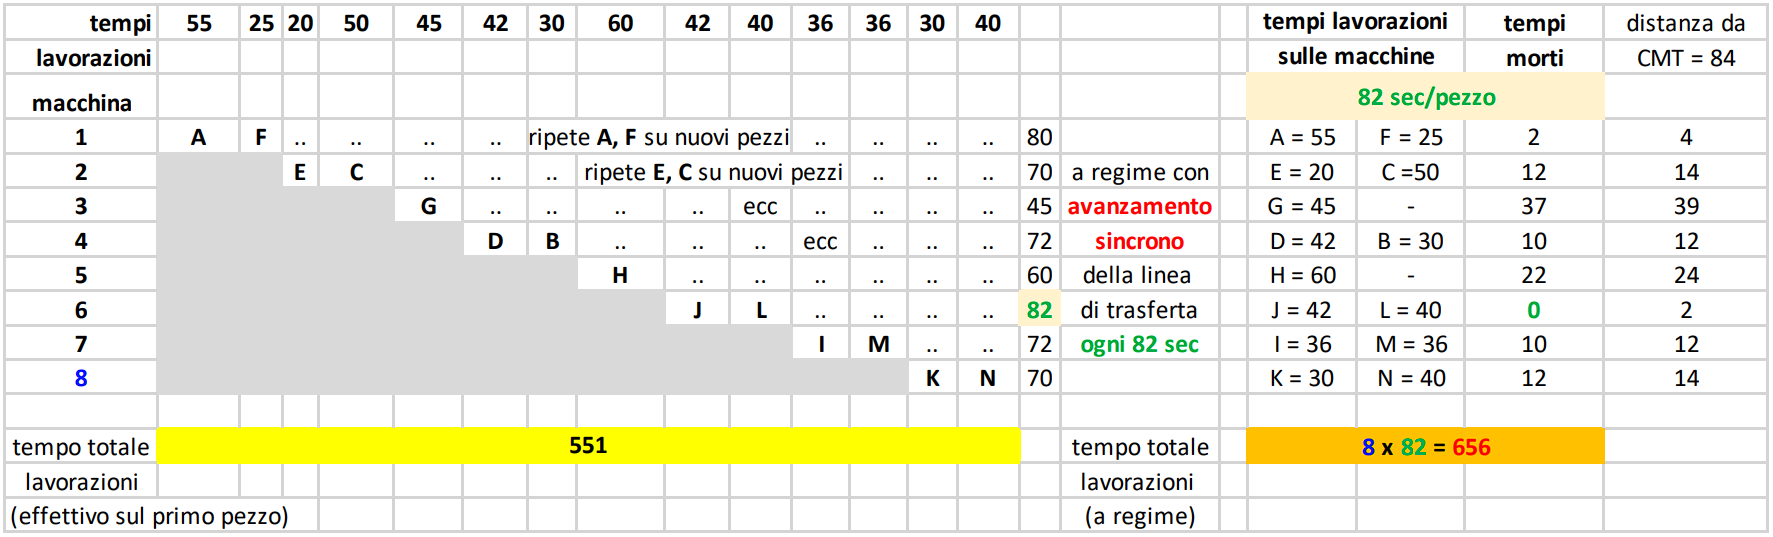
\includegraphics[width=1\textwidth ]{images/gantt.png}
\end{center}
\subsection{Flow Shop}
Un'altro tipo di struttura per un sistema industriale è il già citato flow shop, dove vi è la produzione 
di diversi prodotti, che devono seguire un determinato percorso fra le macchine presenti. Ogni prodotto 
deve vedere $m$ lavorazioni, e differenti prodotti, possono passare per la stessa macchina, ma 
necessitando di tempi differenti, quindi, sarà assegnato un tempo di lavorazione ad ogni 
coppia (lavorazione, prodotto). Il tempo totale di completamento $T_{max}$, detto \textbf{makespan}, è il 
valore da minimizzare, possono essere presenti dei buffer nella struttura.\acc Il problema si complica 
rispetto la linea di trasferta, in questo caso però, date per assunte delle condizioni, vi è una regola che permette 
di stabilire una sequenza ottimale.\acc 
\teo{(Regola di Johnson)}
Si considera l'assunzione per cui ci sono esclusivamente 2 macchine/stazioni, denotate $M_1$ e $M_2$.\\
Sia $L=\{l_1,l_2\dots,l_n\}$ un insieme di lavorazioni, i  cui tempi per $M_1$ sono 
$\{t_{1_1},t_{2_1}\dots,t_{n_1}\}$, e i tempi per $M_2$ sono 
$\{t_{1_2},t_{2_2}\dots,t_{n_2}\}$. dove $\forall i, \ t_{i_1}>0\land t_{i_2}>0$. Nella \textbf{soluzione ottimale}, 
la lavorazione $l_i$ precede la lavorazione $l_j$ se e solo se 
$$ \min(t_{i_1},t_{j_2})<\min(t_{j_1},t_{i_2})$$
Tale teorema fornisce una procedura per trovare una soluzione ottimale, i passi sono i seguenti \begin{enumerate}
    \item si costruisce $S1=\{l_i\in L \ | \ t_{i_1}<t_{i_2}\}$ (lavorazioni più rapide su $M_1$)
    \item si costruisce $S2=S1^C=\{l_i\in L \ | \ l_i\notin S1\}$ (lavorazioni più rapide su $M_2$)
    \item Vengono schedulate le lavorazioni secondo la regola\begin{itemize}
        \item prima si eseguono tutte le lavorazioni di $S1$ in ordine crescente secondo $t_{i_1}$
        \item poi si eseguono tutte le lavorazioni di $S2$ in ordine decrescente secondo $t_{i_2}$
    \end{itemize}
\end{enumerate}
\subsubsection{Esempio di Applicazione per 2 Macchine}
Si hanno le seguenti lavorazioni \begin{center}
    \begin{tabular}{|c|c|c|c|c|c|c|}
        \hline
        Lavorazione & A & B & C & D  & E  & $T_{tot}$ \\ \hline
        $t_{i_1}$   & 5 & 3 & 8 & 10 & 7  & 33        \\ \hline
        $t_{i_2}$   & 2 & 6 & 4 & 7  & 12 & 31        \\ \hline
        \end{tabular}
\end{center}
Si costruiscono i due insiemi\begin{itemize}
    \item $S1=\{B, E\}$
    \item $S2=\{A, C, D\}$
\end{itemize}
Si ordinano secondo i criteri della procedura ottenendo la sequenza $$ S^* = 
B\rightarrow E\rightarrow D \rightarrow C \rightarrow A$$\begin{center}
    \includegraphics[width=0.8\textwidth ]{images/jhonson.eps}
\end{center}
Gli intervalli rossi nella linea del tempo rappresentano il \textit{tempo sprecato},
all'istante $t=20$, la lavorazione D termina su $M_1$, ed è pronta ad essere schedulata 
su $M_2$, ma quest'ultima è ancora impegnata nella lavorazione di E, per questo il prodotto 
che ha appena terminato D dovrà attendere, sarà quindi necessaria la presenza di un buffer. Situazione analoga 
per la lavorazione C nell'istante 28. \acc 
Non ci sono attese sulla macchina 1, le attese sulla macchina 2 sono inevitabili, ma tale procedura 
le minimizza. La macchina 1 è costantemente carica, si dice che $T_{idle,1}=0$ (non ci sono tempi di attesa). 
Differente è la situazione per la macchina 2 : $T_{idle,2}=4$. Il tempo di lavorazione totale è $T_{max}=35$.
\subsubsection{Generalizzazione con 3 Macchine}
Sotto ulteriori ipotesi, è possibile trovare una soluzione ottimale anche in un contesto con 3 macchine (o stazioni) $M_1,M_2,M_3$, 
con relativi tempi di lavorazione $t_{i_1},t_{i_2},t_{i_3}$ con $i\in\{1,2\dots ,n\}$ dove $n=$numero 
lavorazioni. Per poter 
trovare tale soluzione, è necessario che venga soddisfatta la seguente condizione 
$$ \max_{i\in\{1,2\dots ,n\}}(t_{i_2})\le \min_{i\in\{1,2\dots ,n\}}(t_{i_1}) \ \lor  
\max_{i\in\{1,2\dots ,n\}}(t_{i_2}) \le \min_{i\in\{1,2\dots ,n\}}(t_{i_3}) $$
Se tale condizioni è avverata, è possibile considerare una struttura flow shop a due macchine, precisamente $M'_1,M'_2$, con le 
medesime lavorazioni, la cua soluzione è identica alla soluzione del sistema originale con 3 macchine.\acc 
Nel nuovo sistema, i nuovi tempi di lavorazione $t'_{i_1},t'_{i_2}$ vanno definiti come segue \begin{itemize}
    \item $t'_{i_1}=t_{i_1}+t_{i_2}$
    \item $t'_{i_2}=t_{i_2}+t_{i_3}$
\end{itemize}
\subsubsection{Esempio di Applicazione per 3 Macchine}
Si hanno le seguenti lavorazioni \begin{center}
    \begin{tabular}{|c|c|c|c|c|}
        \hline
        Lavorazione & A & B & C & D \\ \hline
        $t_{i_1}$   & 4 & 1 & 5 & 2 \\ \hline
        $t_{i_2}$   & 3 & 2 & 3 & 3 \\ \hline
        $t_{i_3}$   & 3 & 4 & 5 & 3 \\ \hline
        \end{tabular}
\end{center}
La condizione $\max_{i\in\{1,2\dots ,n\}}(t_{i_2}) \le \min_{i\in\{1,2\dots ,n\}}(t_{i_3}) $ è soddisfatta, 
quindi è possibile ridurre il sistema ad uno equivalente \begin{center}
    \begin{tabular}{|c|c|c|c|c|}
        \hline
        Lavorazione & A & B & C & D \\ \hline
        $t_{i'_1}$   & 7 & 3 & 8 & 5 \\ \hline
        $t_{i'_2}$   & 6 & 6 & 8 & 7 \\ \hline
        \end{tabular}
\end{center}
Si applica la regola di Johnson, trovando la sequenza $S^*=B\rightarrow D\rightarrow C\rightarrow A$, che verrà 
applicata al sistema originale con 3 macchine.\begin{center}
    \includegraphics[width=0.9\textwidth ]{images/jhonson2.eps}
\end{center}
Un altra struttura è la \textbf{produzione per reparti}, già accennata con il nome di \textbf{job shop},
in cui l'impianto è suddiviso in reparti contenenti stazioni, ed i vari prodotti devono essere passati fra i 
reparti attraverso sistemi di trasporto che seguono un percorso 
prefissato, è quindi necessario considerare il routing dei prodotti fra i reparti. Il modello job shop è caratterizzato 
da \begin{itemize}
    \item vaste categorie di prodotti, che subiscono lavorazioni con sequenze differenti 
    \item operazioni non ripetitive ed alta flessibilità 
    \item un maggiore work in process, i flussi lavorativi sono intricati 
    \item elevati tempi di attraversamento, e qualità dei prodotti non sempre omogenea
\end{itemize}
Quando è possibile individuare famiglie di prodotti simili con cicli di lavorazione omogenei, si identificano delle 
celle contenenti gruppi di macchine adatti a tale famiglia di prodotti, tale \textbf{produzione per celle} semplifica 
i flussi di produzione, il trasporto e la gestione, le varie celle sono indipendenti fra loro.\acc
\begin{figure}[h!]
    \centering
    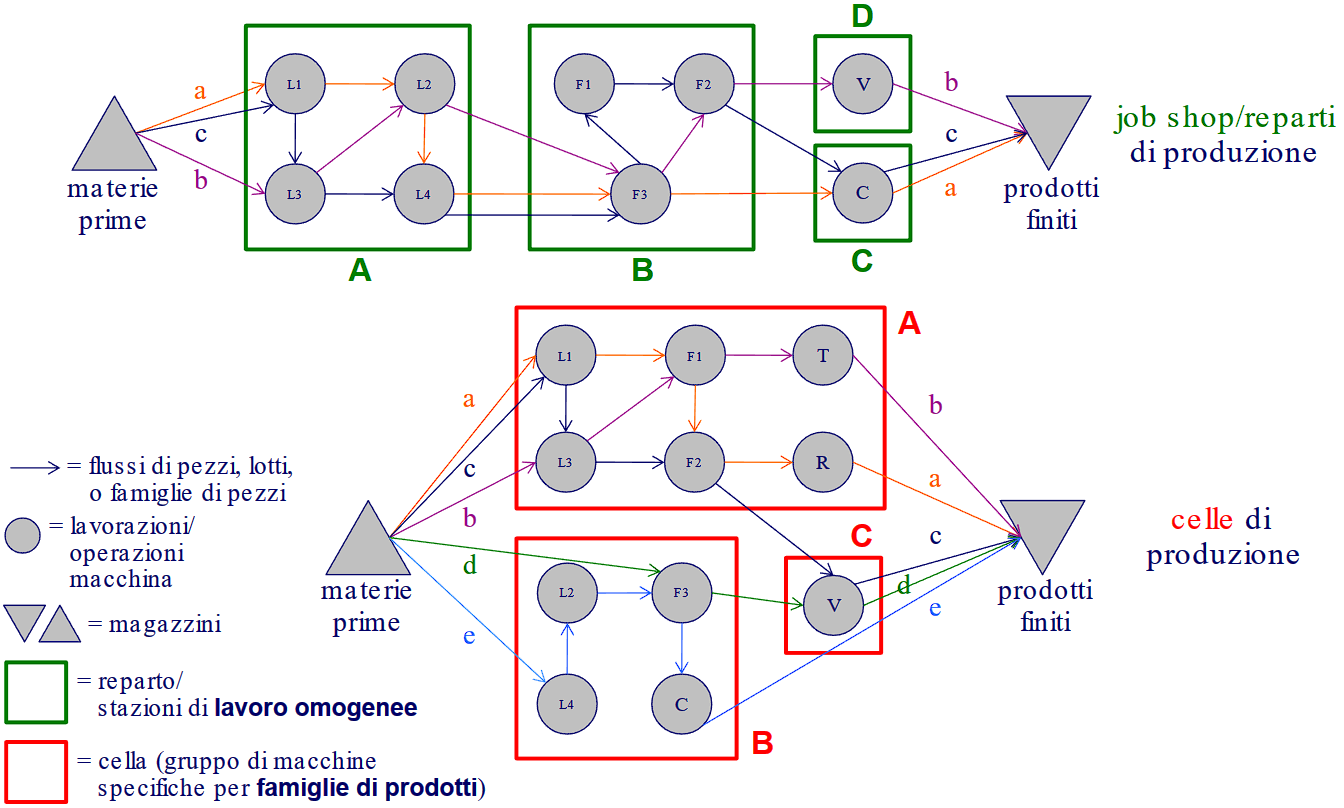
\includegraphics[width=0.65\textwidth ]{images/celleReparti.png}
    \caption{job shop e celle di produzione}
\end{figure}
Quando si implementa il trasporto automatico ed un controllo tramite calcolatore nelle celle di produzione si 
parla di \textbf{Flexible Manufacturing/Assembly Systems (FMS/FAS)}, sono sistemi dotati di elevata 
 flessibilità riguardo alle diverse sequenze delle lavorazioni 
 e/o all'assegnamento di operazioni alle risorse. Sono caratterizzati da \begin{itemize}
    \item diversi prodotti 
    \item lavorazioni eseguite su più macchine 
    \item assegnazione delle risorse tramite routing dei flussi 
    \item problemi di sequenziamento locale dell'impiego delle risorse 
    \item alto grado di automazione
 \end{itemize}
È possibile individuare tre tipi di automazione industriale\begin{itemize}
    \item \textit{Automazione rigida} : La sequenza delle operazioni è fissata, sono sistemi poco 
     flessibili (come le linee di trasferta) destinati a grandi produzioni con poca varietà di prodotto.
    \item \textit{Automazione programmabile} : Si può cambiare la configurazione del flusso di produzione in modo 
    da variare il prodotto, tipico delle industrie con produzione discreta a lotti. Vi è un tempo di attesa 
    fra un lotto ed un altro per la riconfigurazione del flusso.
    \item \textit{Automazione flessibile} : estensione dell'automazione programmabile in 
    cui è possibile diversificare la produzione senza avere tempi morti di 
    conversione dell'impianto,  i macchinari utilizzati sono caratterizzati da un alta configurabilità.
\end{itemize}
In generale, per i sistemi di automazione, esiste una correlazione qualitativa fra la quantità di prodotto fabbricata, ed il 
numero di prodotti distinti.\begin{center}
    \includegraphics[width=1\textwidth ]{images/quantitVarieta.eps}
\end{center}\flowerLine 
\section{Sistema di Supporto}
Un sistema di supporto consiste in un insieme di attività legate all'impianto di produzione, in particolare\begin{itemize}
    \item attività di business, quali gestione degli ordini, marketing del prodotto e considerazioni economiche 
    \item progettazione del prodotto sulla base delle esigenze del mercato 
    \item pianificazione ("planning") della produzione, definizione della sequenza di lavorazione, politiche 
    di stoccaggio e rifornimento 
    \item controllo delle attività (gestione e supervisione)
\end{itemize}
Tali attività si re-iterano in un ciclo di produzione, cosiddetto "agile".
\begin{center}
    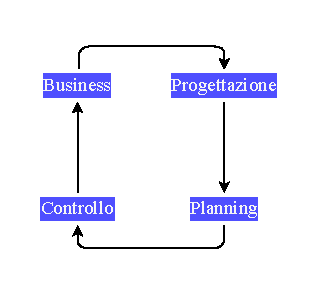
\includegraphics[width=0.3\textwidth ]{images/sistSupp.pdf}
\end{center}
In supporto delle attività di business vi sono \begin{itemize}
    \item \textbf{Enterprise Resource Planning (ERP)} : Un insieme di software volti all'automazione 
    dell'amministrazione, della logistica, della produzione e delle risorse umane. 
    \item \textbf{Decision Support System (DSS)} : Sistemi che hanno lo scopo, dato un insieme di dati 
    e dei vincoli da rispettare, di migliorare il processo decisionale nell'impianto.
\end{itemize}
Inoltre le macchine sul campo vengono supportate da sensori che hanno lo scopo di raccogliere dati ed informazioni 
in maniera massiva, in modo da poter essere utilizzati per i modelli di intelligenza artificiale e machine learning, 
sfruttando appunto,  tali dati per effettuare previsioni con maggiore precisione.
\acc In supporto alle attività di progettazione vi sono \begin{itemize}
    \item \textbf{Computer Aided Design (CAD)} : Un insieme di strumenti informatici utili nella progettazione. 
    \item \textbf{Computer Aided Engineering (CAE)} : Un insieme di strumenti informatici utili nella verifica 
    delle funzionalità tramite simulazioni e modelli matematici.
    \item \textbf{Computer Aided Manufacturing (CAM)} : Un insieme di software utili nell'automatizzazione ed 
    organizzazione delle sequenze di operazioni nella produzione.  
    \item \textbf{Computer Aided Process Planning (CAPP)} : software che 
    permette di automatizzare/ottimizzare il planning della produzione
\end{itemize}
È possibile utilizzare un modello CAD per ottenere un programma da eseguire su una CNC (macchina a controllo numerico)\begin{itemize}
    \item Caricamento di un modello CAD 
    \item Impostazione del sistema di coordinate 
    \item Impostazione di parametri 
    \item Generazione delle istruzioni per la macchina in questione 
    \item Invio dei dati al controllo numerico
\end{itemize}
\flowerLine 
\section{La Piramide CIM}
Quello della piramide CIM è un modello teorico che descrive la struttura di un processo produttivo, integrata 
con i sistemi di automazione ed i sistemi informatici gestionali, tale modello propone diversi vantaggi\begin{itemize}
    \item miglioramento della qualità di produzione 
    \item tempi e costi ridotti 
    \item aumento della flessibilità 
    \item diminuzione degli scarti e manutenzione predittiva 
    \item fondamentale per conformarsi a leggi e regolamenti sulla 
    sicurezza del processo produttivo, sulla qualità del prodotto e sulla riduzione dell'impatto ambientale
\end{itemize}
Il modello CIM è gerarchico e suddivide il processo di produzione su vari livelli, i cui elementi comunicano 
orizzontalmente con quelli adiacenti. Ogni livello assume che l'automazione nel livello inferiore sia 
ideale, nessun livello è privilegiato rispetto ad un altro.\begin{center}
    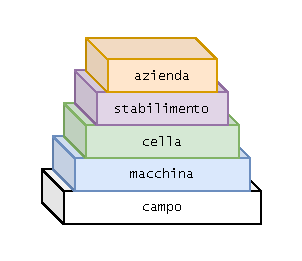
\includegraphics[width=0.6\textwidth ]{images/cim.pdf}
\end{center}
Dai livelli superiori le informazioni sono più elaborate e di minore quantità, ed i comandi vengono dati con minore 
frequenza, nei livelli inferiori, ci sono 
più informazioni, ma sono semplici, ed i comandi vengono dati con maggiore 
frequenza. La comunicazione verticale è privilegiata, se più dispositivi di campo devono 
comunicare, devono farlo attraverso il sistema di controllo della macchina di cui fanno parte. \acc 
Al livello di macchina e campo il controllo può essere sia \textit{logico} che \textit{diretto} (real time), 
attuato da microprocessori, con il salire dei livelli nella piramide il controllo assume sempre più un carattere 
logico, dettato da eventi.
\subsection{Livelli della Piramide}
\subsubsection{Livello di Campo}
Tale livello contiene dispositivi quali sensori ed attuatori, in generale,  i componenti hardware che 
eseguono le attività di produzione e controllo. Tali dispositivi interfacciano il livello superiore al livello 
fisico tramite segnali di ingresso ed uscita, possono inoltre comunicare informazioni sul proprio 
stato (auto diagnosi), oltre a ciò, sono generalmente semplici.\acc 
Sono raggruppati in semplici sistemi di controllo e i livelli superiori li assumono come dispositivi 
ideali, sono attrezzati di apposito hardware di controllo, quali sistemi digitali a microprocessori/sistemi 
embedded.
\subsubsection{Livello di Macchina}
Una macchina raggruppa più dispositivi di campo volti al fornire una determinata funzionalità. Ad esempio, 
diversi motori elettrici (dispositivi di campo) possono costituire un braccio robotico (macchina) volto allo 
spostamento di oggetti.\acc 
Tali componenti vengono controllati tramite dei controllori logici programmabili (PLC), tramite la regolazione 
di variabili analogiche e la realizzazione di sequenze di operazioni.\begin{quote}
    \color{gray}
    esempio: a livello di campo si controllano le posizioni dei singoli giunti; a livello di macchina 
viene pianificato il movimento del robot nello spazio operativo e la sequenza delle azioni che 
deve effettuare
\color{black}\end{quote}
\subsubsection{Livello di Cella}
Diverse macchine vengono raggruppate insieme formando delle celle di produzione, atte a produrre prodotti, anche 
diversi ma tecnologicamente affini, le macchine sono interconnesse fisicamente da un sistema locale di trasporto 
e stoccaggio. Nonostante il vincolo real time sia presente, il livello di controllo è quasi 
esclusivamente logico, e coordinano le macchine della cella. 
\subsubsection{Livello di Stabilimento}
Racchiude più celle e linee produttive di un impianto industriale, riceve istruzioni dal livello gestionale e le 
attua sotto forma di piani operativi per la produzione. I sistemi di controllo a tale livello sono denominati 
\textit{SCADA (Supervisory Control And Data Acquisition)}, tipicamente implementati in workstation. Sono sistemi di 
controllo che dispongono di\begin{itemize}
    \item Un interfaccia con l'operatore, assente nei microcontrollori e nei PLC 
    \item Gestione di allarmi e ricette 
    \item Programmazione dei lavori e basi di dati del processo produttivo 
    \item Controllo statistico e supporto alla manutenzione, potendo fare previsioni e rapporti
\end{itemize}
\begin{figure}[h!]
    \centering
    \includegraphics[width=0.65\textwidth ]{images/centrale (2).png}
    \caption{sala di controllo di una centrale elettrica}
\end{figure}
\subsubsection{Livello di Azienda}
Si occupa dei processi gestionali, il sistema non è di controllo ma \textit{decisionale}, costituito da un 
infrastruttura software connessa al mainframe aziendale, non esistono vincoli di tipo temporale.\acc 
Esiste uno standard (ANSI/ISA-S88.01-1995) che normalizza lo schema generale di controllo su 3 livelli gerarchici.
\begin{figure}[h!]
    \centering
    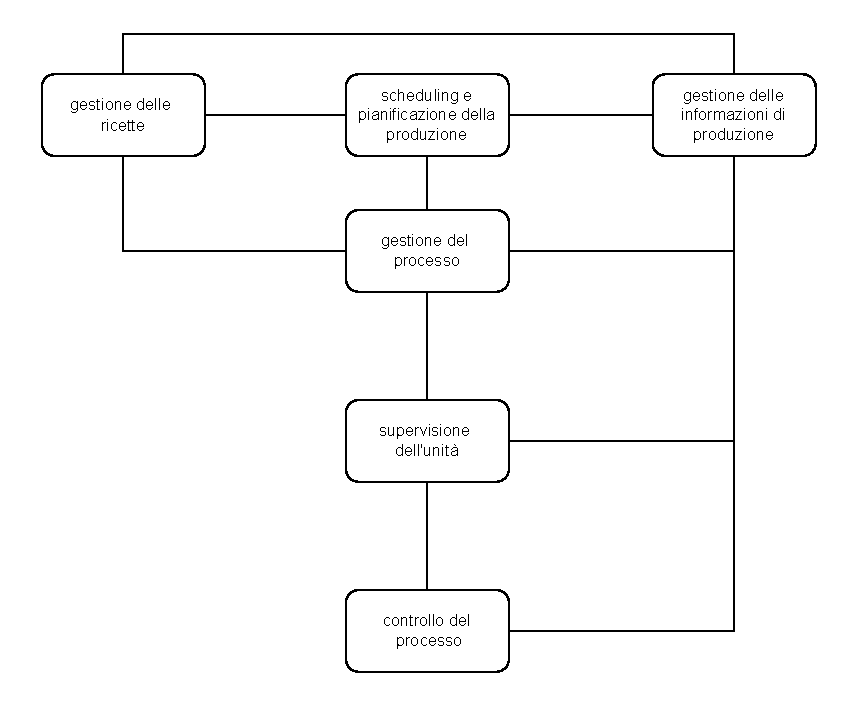
\includegraphics[width=0.7\textwidth ]{images/standardControlModel.pdf}
    \caption{modello delle attività di controllo}
\end{figure}
\begin{itemize}
    \item \textbf{controllo di campo} : controllo che agisce sui dispositivi di campo, in particolare, 
    su variabili continue, ed è implementato  su dispositivi dedicati. Le informazioni sono semplici 
    e trasmesse ad alta frequenza. 
    \item \textbf{controllo di procedure} : riguarda il controllo dei livelli di macchina e cella della 
    piramide, riguarda gruppi strutturati di componenti di campo, a tale livello vengono svolte funzioni di 
    auto-diagnostica, è implementato su schede dedicate o anche su pc industriali. Prevede 
    algoritmi più complessi di quelli del controllo di campo. Il controllo è \begin{itemize}
        \item \textit{diretto} : riguarda il controllo di 
        gruppi di variabili continue o funzioni più avanzate 
        \item \textit{logico} : coordinamento dei sistemi di campo sulla base della lista 
        di operazioni sequenziali
    \end{itemize}
    \item \textbf{controllo di coordinamento} : si pone al livello dello stabilimento ed opera su dati 
    strutturati a bassa frequenza, riguarda il coordinamento e la gestione delle varie celle di produzione, vincoli 
    temporali molto laschi.
\end{itemize}
\begin{center}
        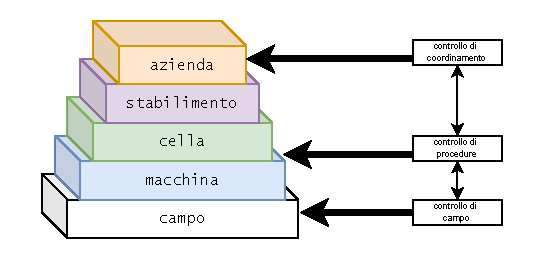
\includegraphics[width=0.7\textwidth ]{images/cim2.pdf}
\end{center}
Lo standard definisce anche un diagramma logico delle transizioni tra stati di un processo. Si noti come 
i due stati \textit{Held} e  \textit{Paused} sono differenti: \begin{itemize}
    \item \textit{Paused} : è scaturita da un operatore esterno (esempio : causa operazioni di verifica) 
    \item \textit{Held} : il processo è in attesa di un evento e viene bloccato
\end{itemize}
\begin{center}
    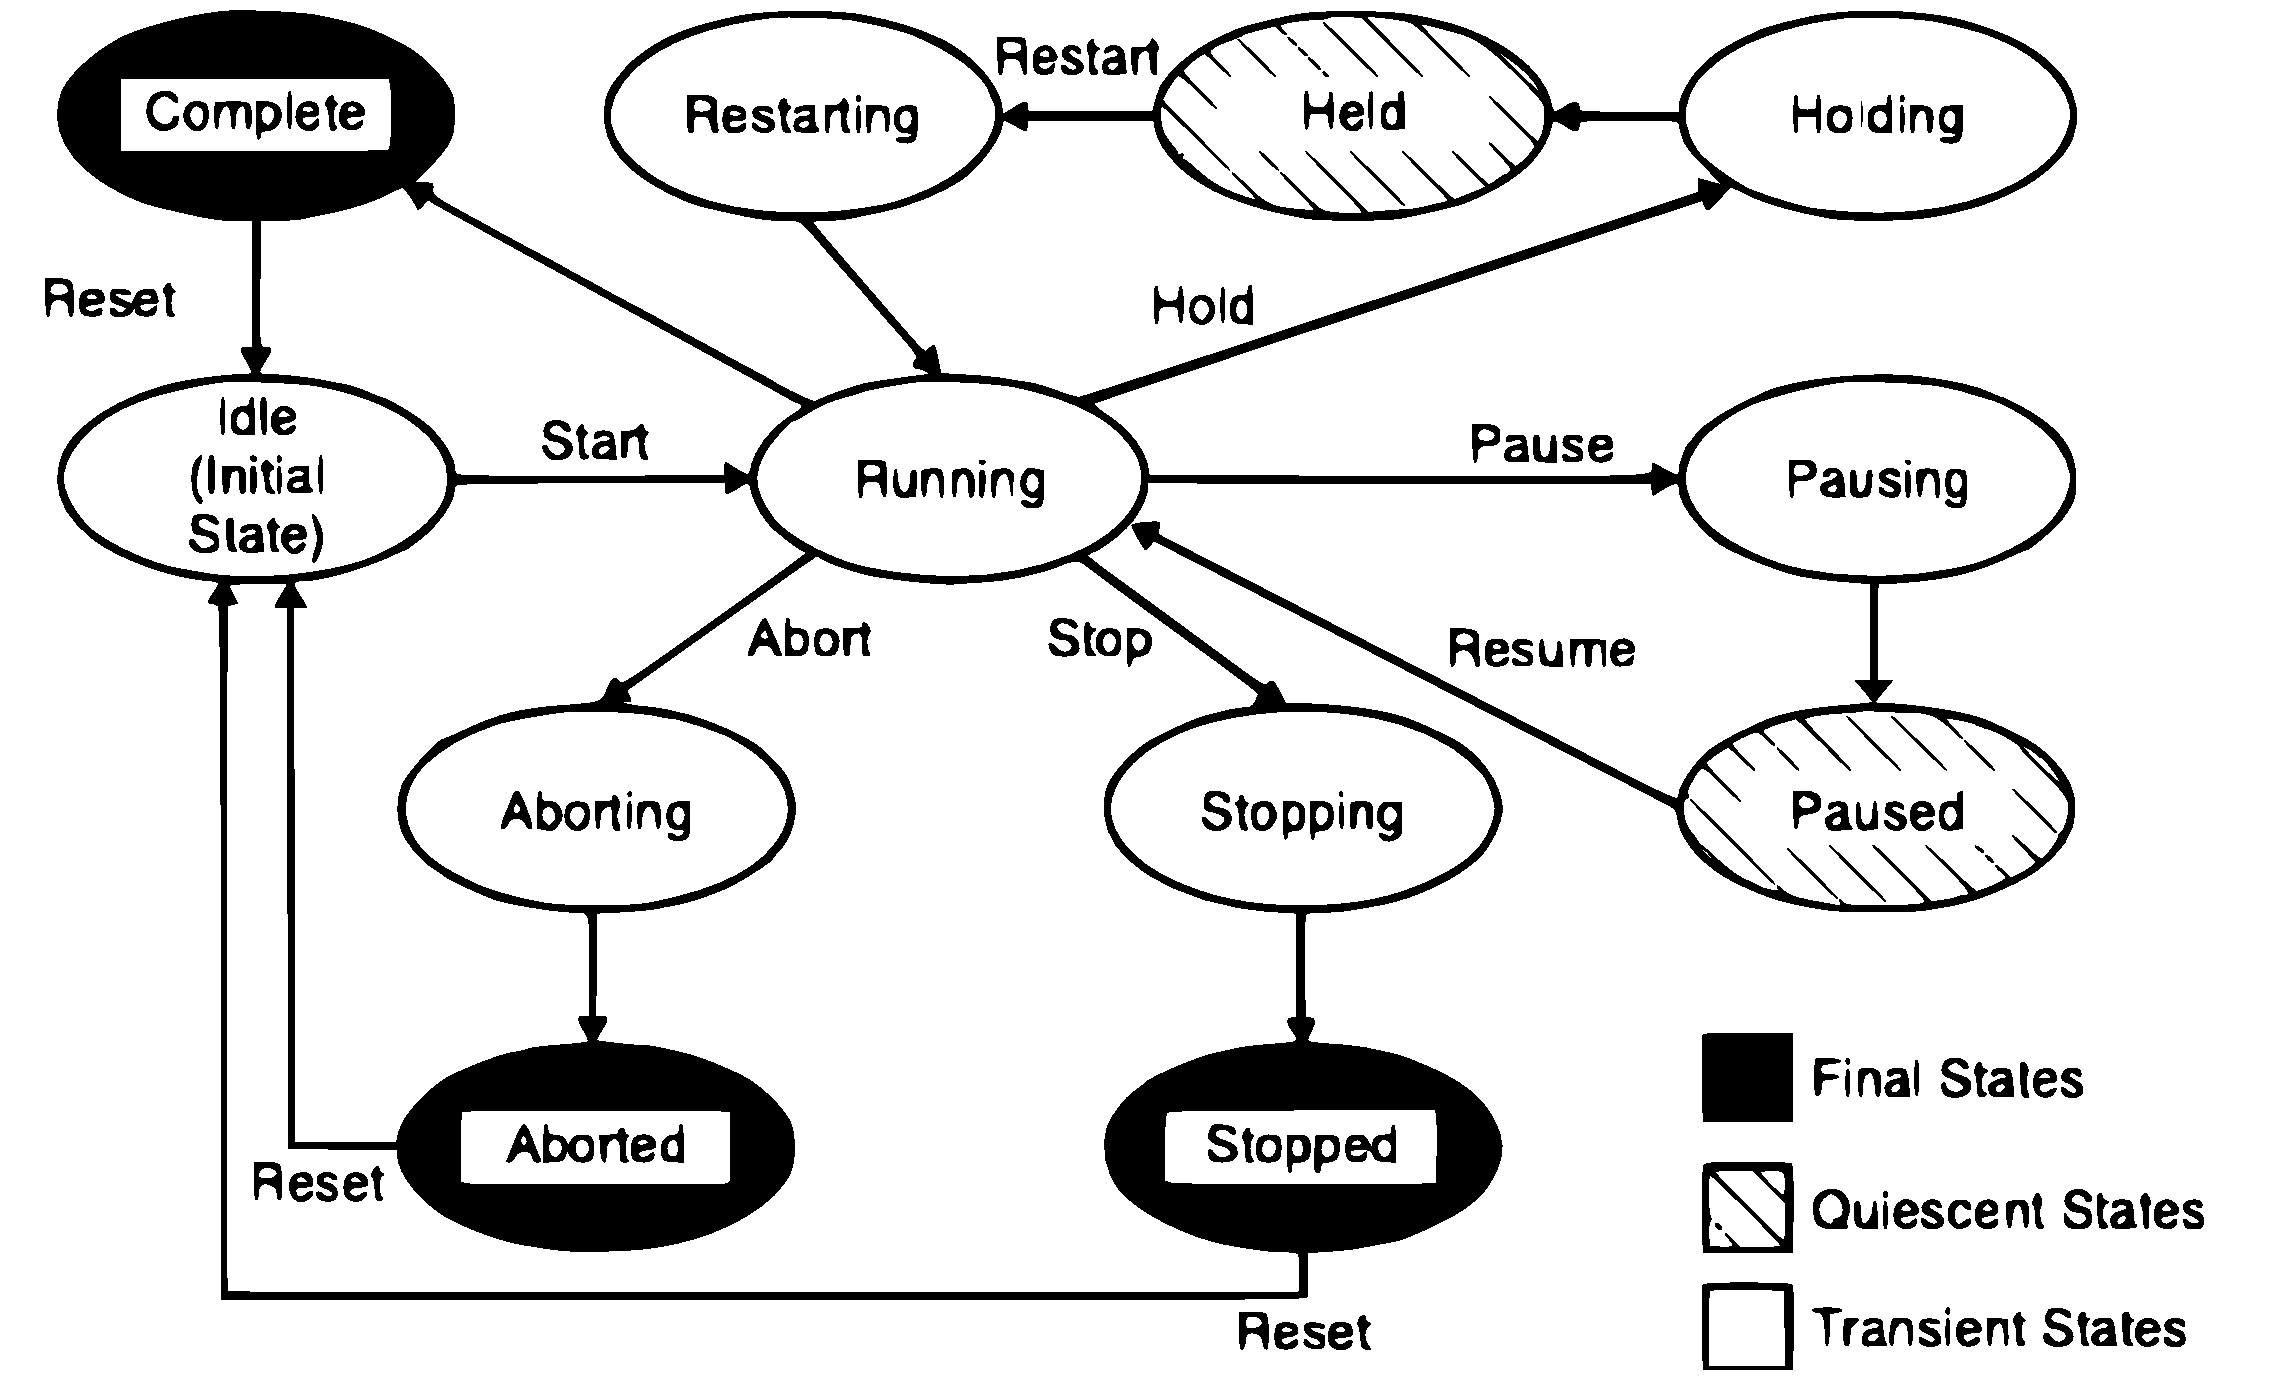
\includegraphics[width=0.7\textwidth ]{images/statiProcesso.pdf}
\end{center}
\subsection{Auto-diagnostica}
I sistemi di controllo devono avere la possibilità di generare segnali ausiliari che danno allarme di eventuali guasti 
nei dispositivi soggetti ad usura. Occorre individuare dei segnali dal dispositivo che possono essere 
valutati secondo appropriati modelli matematici. \acc 
Con \textit{signature}, si definisce una firma del guasto, ossia una sua manifestazione sottoforma di segnale, un esempio 
può essere la misura tramite un accelerometro di vibrazioni in un sistema meccanico. Si sviluppano algoritmi atti 
all'analisi dei segnali (basati ad esempio sulla trasformata di Fourier).\acc 
Definiamo \textit{fault} i guasti, e li denotiamo $f$, su di essi si formulano\begin{itemize}
    \item \textit{fault detection} : rilevamento dei guasti sul sistema fisico o software 
    \item \textit{fault isolation} : classificazione del guasto, e distinzione di esso rispetto ad altri 
    \item \textit{fault identification} : determinazione del profilo temporale del guasto $f$ 
    \item \textit{fault accomodation} : riconfigurazione a seguito del guasto, coinvolge modifiche hardware o software
\end{itemize}
\subsubsection{Rilevazione ed Isolazione }
Quando un sistema dinamico è soggetto ad un possibile guasto, si definisce un sistema ausiliario detto 
\textbf{generatore di residuo}, il cui segnale in uscita dipenderà dalla presenza di un particolare guasto 
$f$. \begin{quote}
    Un residuo $r$ dipende da un guasto $f$
\end{quote}
Nel caso in cui possono esserci più guasti, si definisce un vettore $\bar r$ di residui, in cui $r_i$ dipende 
da $f_i$. Tipicamente il residuo riproduce approssimativamente  l'evoluzione temporale del guasto. Con FDI si intende l'operazione 
di "Fault Detection Isolation", queste ultime due possono avvenire in contemporanea, vi sono differenti modelli proposti\begin{itemize}
    \item \textit{model-based} : si definisce un sistema dinamico che rappresenta il guasto (generatore di residuo)
    \item \textit{signal-based} : si utilizzano esclusivamente i segnali provenienti da misure del sistema, la loro 
    elaborazione può far luce su eventuali guasti 
    \item \textit{ibrido} : si combinano entrambe le tecniche
\end{itemize}
\subsubsection{Esempio di Residuo}
Vi è un processo (soggetto a guasto) modellato dal seguente sistema dinamico$$\begin{cases}
    \dot{x}=ax+bu+ef\\y=cx
\end{cases} $$
Dove $f$ è il generico fault. Il residuo $r$ viene implementato come osservatore di un disturbo, o di un 
segnale non noto (che in questo caso è $f$).  Rappresenta proprio la stima del disturbo al tempo $t$.
$$ r(t)=\frac{k}{e}\Big[
\frac{y(t)}{c}-\int_0^t[ax(\tau)+bu(\tau)+er(\tau)d\tau]\Big] \ \  \text{ con }\ \ \begin{matrix}
    k>0\\ r(0)=0
\end{matrix}    
$$
L'integrale indica che la stima del disturbo viene calcolata tenendo conto di tutti i valori passati del disturbo stesso.\acc 
Il parametro $k$ è un guadagno che determina quanto "velocemente" l'osservatore reagisce ai cambiamenti del disturbo. Un valore di $k$ più alto significa una risposta più rapida, ma può anche introdurre più rumore nella stima.
L'evoluzione nel tempo del residuo è data da 
\begin{eqnarray}
    \dot{r}=\frac{k}{e}\Big[ \frac{\dot{y}}{c}-[ax+bu+er] \Big] = \\
    \frac{k}{e}\Big[ \frac{c[ax+bu+ef]}{c}-[ax+bu+er] \Big] = \\
    \frac{k}{e}e[f-r] = k[f-r]
\end{eqnarray}
Si ha quindi l'equazione lineare del primo ordine 
$$ kr+\dot{r}-kf=0$$
Si porta nel dominio di Laplace 
$$\mathcal{L}[kr+\dot{r}-kf](s)= $$ $$ 
k\mathcal{L}[r](s)+
\mathcal{L}[\dot{r}](s)-
k\mathcal{L}[f](s) = 
$$$$ 
k\mathcal{L}[r](s)+
s\mathcal{L}[r](s)-r(0)-
k\mathcal{L}[f](s) = 
$$
Si ricordi come $r(0)=0$. Denoto $\mathcal{L}[f]=F$ e $\mathcal{L}[r]=R$
$$ 
kR(s)+sR(s)-kF(s)=0\implies 
$$ $$ 
R(s)[k+s]=kF(s)
$$ 
$$
R(s)=\frac{kF(s)}{k+s} \implies 
$$ 
$$ \frac{R(s)}{F(s)}=\frac{k}{k+s}=\frac{1}{1+\frac{1}{k}s} $$
Nel caso il guasto fosse costante $f(t)=f_0$, nel dominio del tempo si avrebbe 
$$ r(t)=f_0[1-e^{-kt}]$$
\subsection{Architetture per il Controllo}
Il controllo è gestito da dispositivi elettronici ed informatici, è possibile individuare 3 tipi di 
sistemi\begin{itemize}
    \item \textbf{controllori embedded} - per il controllo di campo 
    \item \textbf{architettura a bus} - per il controllo di procedure 
    \item \textbf{PC-based}
\end{itemize}
\subsubsection{Sistemi Embedded}
Tali sistemi di controllo sono "fusi" alle funzionalità del dispositivo, e sono adoperati per un unico, specifico e 
predeterminato compito. Sono piattaforme hardware create "ad hoc", e la loro progettazione dipende dalla conoscenza dei 
compiti che dovranno svolgere. La realizzazione può avvenire in due modi \begin{itemize}
    \item singolo chip integrato (microcontrollori)
    \item singola scheda (DSP o FPGA)
\end{itemize}
L'hardware è semplice, vi è una CPU per gli algoritmi, una memoria per i dati ed i programmi e dei circuiti per 
gestire input ed output (analogici o digitali, con eventuali convertitori). Hanno un software integrato molto 
semplice ed è orientato all'automazione, vi è una gestione a basso livello delle risorse e delle comunicazioni.
\subsubsection{Microcontrollori}
I microcontrollori (a singolo chip) sono nati a seguito della miniaturizzazione dell'elettronica, sono 
utilizzati in una grandissima varietà di applicazioni e possono essere integrati con un sistema di sviluppo 
per la loro programmazione.\begin{figure}[h!]
    \centering
    \includegraphics[width=0.7\textwidth ]{images/auto.png}
    \caption{Sistemi di controllo embedded in automotive}
\end{figure}\acc
Caratteristiche ed impieghi : \begin{itemize}
    \item applicazioni semplici 
    \item basso consumo e poco spazio occupato 
    \item numero limitato di segnali da gestire. Interfaccia utente assente 
    \item scarsa integrazione con dispositivi simili, difficile espansione
\end{itemize}
\subsubsection{Singola Scheda}
Prevedono più componenti standard integrati su una singola scheda, fra questi vi sono\begin{itemize}
    \item DSP (Digital Signal Processor) : processori atti al trattamento dei segnali ed esecuzione di funzioni su numeri interi o reali 
    \item FPGA (Field Programmable Gate Array) : circuiti integrati riconfigurabili dall'utente per realizzare 
    funzioni logiche complesse tramite blocchi logici e elementi di memoria
\end{itemize}
Rispetto i microcontrollori hanno una maggiore capacità di elaborazione e possono gestire un maggior numero 
di segnali.\acc 
Ricapitolando, i sistemi di controllo embedded prevedono i seguenti:\begin{itemize}
    \item \textbf{PRO}\begin{itemize}
        \item combinazione hardware/software specificamente studiata 
        \item ottimizzazione spaziale e di complessità
        \item minori ingombri, basso consumo 
        \item minori costi
    \end{itemize}
    \item \textbf{CONTRO}\begin{itemize}
        \item interfaccia uomo-macchina poco evoluta
        \item  gestione di un numero limitato di segnali in input/output 
        \item  costi di progettazione (hardware e software) non irrilevanti 
        \item poca flessibilità: modifiche ai compiti da svolgere possono 
        rendere necessaria la progettazione di un nuovo dispositivo 
    \end{itemize}
    Utili quando i compiti di controllo sono noti a priori.
\end{itemize}
\begin{figure}[h!]
    \centering
    \includegraphics[width=0.7\textwidth ]{images/cellaLogica.eps}
    \caption{cella logica elementare in un FPGA}
\end{figure}
\subsubsection{Architettura a Bus}
Con \textit{bus} si intende una linea elettrica che mette in comunicazione più dispositivi, vi è una scheda madre 
con un bus a cui si connettono più schede, in modo da rendere modulare il sistema. Un bus è composto da diverse 
linee\begin{itemize}
    \item linee dati 
    \item linee indirizzi 
    \item linee di alimentazione 
    \item linee per la comunicazione
\end{itemize}
\begin{figure}[h!]
    \centering
    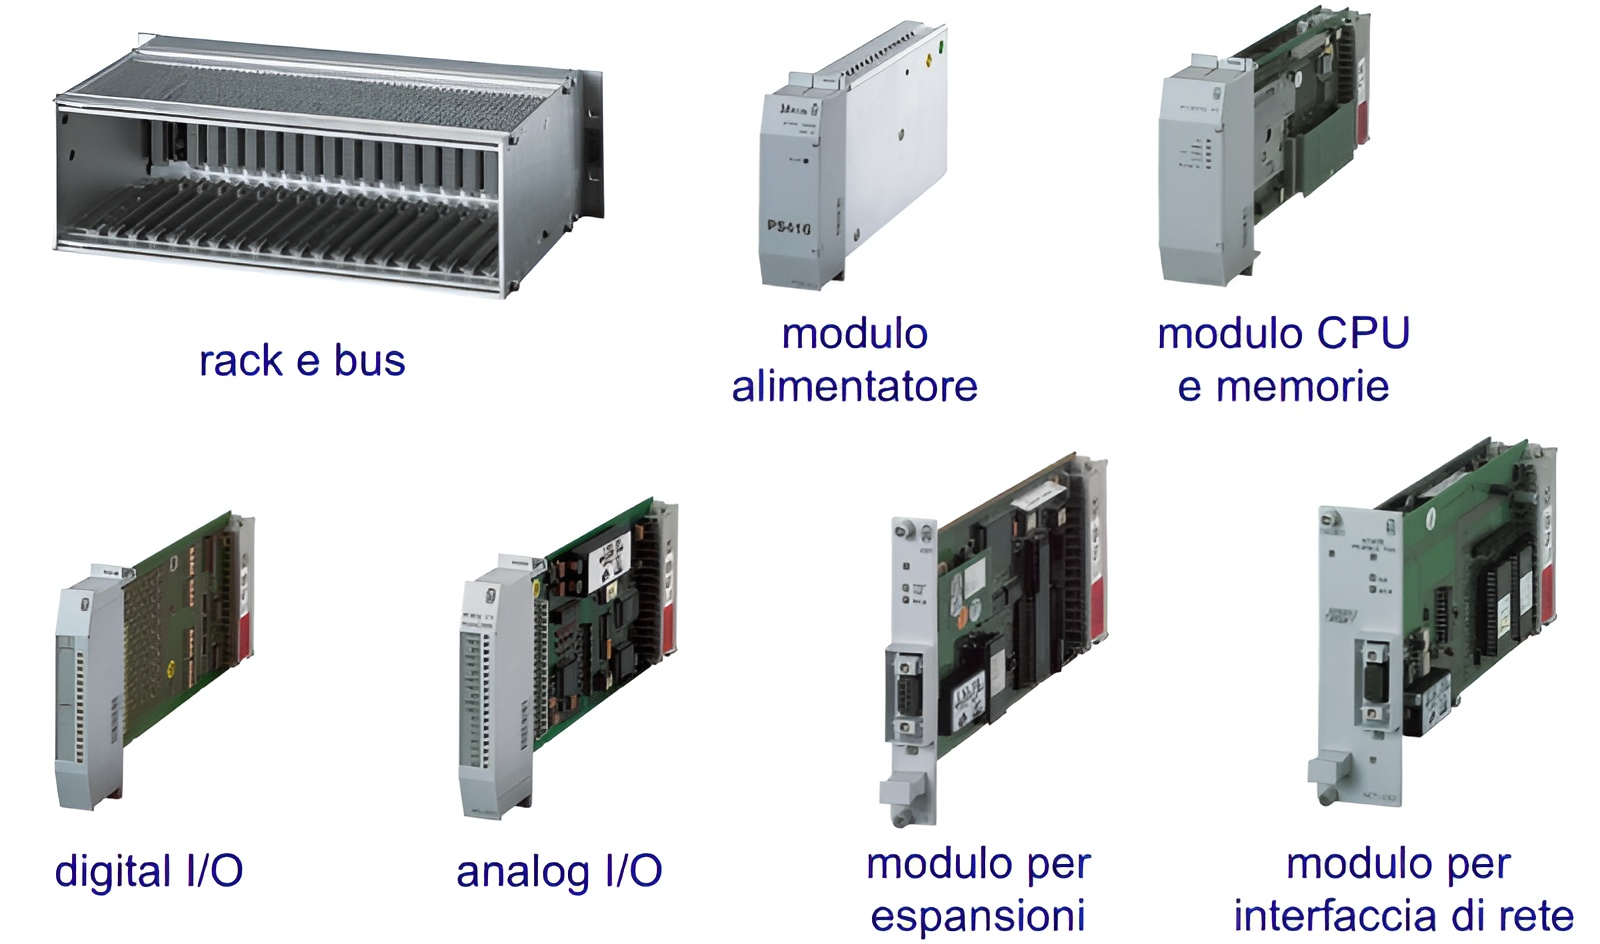
\includegraphics[width=0.6\textwidth ]{images/bus.png}
    \caption{Modularità dell'architettura a bus}
\end{figure}
\begin{itemize}
    \item \textbf{PRO}\begin{itemize}
        \item flessibilità di progettazione 
        \item scelta dei moduli secondo le funzionalità da implementare
    \end{itemize}
    \item \textbf{CONTRO}\begin{itemize}
        \item Sistema Operativo più complesso
        \item  gestione dei moduli interconnessi e delle comunicazioni
        \item  vincoli real-time  
    \end{itemize}
\end{itemize}
\subsubsection{PC-Based}
Ultimamente, anche i comuni computer (corazzati per resistere alle condizioni 
sfavorevoli degli impianti) sono adoperati  come sistemi di controllo, sono sistemi informatici con architettura  
a bus ed implementano una semplice interfaccia uomo macchina, e sono semplici da connettere alle reti informatiche.\acc 
Per far si che risultino efficaci come sistemi di controllo, esistono appositi sistemi operativi atti 
all'utilizzo real time (ad esempio, RTAI-Linux). Implementano 
moduli/schede per l'interconnessione con un elevato numero di 
segnali input/output, inoltre, esistono appositi protocolli per la comunicazione fra PC e PLC.
\flowerLine
\section{Industria 4.0}
La seconda rivoluzione industriale, agli inizi del $XX^\circ$ secolo ha introdotto la produzione di massa e la catena 
di montaggio classica (Ford), nei primi anni 70 l'avvento dei computer e dei robot ha sondato la 
terza rivoluzione industriale, ad oggi vige l'industria 4.0 in cui le tecnologie ICT (Information and Communication Technology)
pervadono i processi produttivi. Anche la presenza di dispositivi intelligenti (IOT) capaci di fornire dati 
sulla rete tramite sensori e comunicare in tempo reale ha modificato il modo di produrre.\acc 
\textbf{Industria 4.0}:\begin{quote}
    \textit{“the comprehensive transformation of the whole sphere of
industrial production through the merging of digital technology and
the internet with conventional industry”} \\(Angela Merkel - Organization for
Economic Cooperation and Development, 19 Febbraio 2014)
\end{quote}
L'avvento di tali tecnologie ha portato un cambiamento industriale ma  anche sociale, e sono diventate necessarie 
diverse figure professionali che richiedono abilità trasversali per gestire le nuove tecnologie. Definiamo le seguenti, 
\textbf{tecnologie abilitanti}\begin{itemize}
    \item \textit{Soluzioni manufatturiere avanzate} : utilizzo dei robot interconnessi e riprogrammabili 
    nell'automazione di attività precedentemente non automatizzabili.
    \item \textit{Additive manufacturing} : produzione per "addizione" di materiale, resa possibile dalle stampanti 
    3D connesse ai sistemi CAD. 
    \item \textit{Realtà aumentata} : l'uso della realtà aumentata e della realtà virtuale ha permesso la 
     simulazione di processi fisici a supporto dei processi produttivi. 
     \item \textit{Simulazione} : Simulazione in tempo reale del sistema di produzione in grado di 
        migliorare il processo decisionale e predittivo tramite l'uso dei digital twin.
    \item \textit{Integrazione orizzontale/verticale} : Integrazione di informazioni lungo la catena del valore, dal consumatore 
    al fornitore. 
    \item \textit{Internet industriale} : Comunicazione multidirezionale diffusa tra processi produttivi e prodotti. 
    \item \textit{Cloud} : Uso del cloud per la raccolta dei dati in maniera distribuita.  
    \item \textit{Sicurezza} : Metodologie di difesa alle minaccie informatiche alla quale sono soggetti i 
    sistemi aperti ed interconnessi.  
    \item \textit{Big data} : Uso dei modelli volti all'analisi statistica, che sfruttano le grandi quantità di dati 
    disponibili allo scopo di estrarne informazioni. 
\end{itemize}
L'uso delle tecnologie abilitanti porta vari benefici\begin{itemize}
    \item Flessibilità nella produzione di piccoli lotti ai costi della grande scala 
    \item Maggiore velocità della progettazione e produzione dei prodotti 
    \item Maggiore produttività e riduzione dei tempi morti (tempi di setup, errori e fermi macchina)
    \item Migliore qualità del prodotto e riduzione degli scarti grazie a sensori che monitorano la produzione in tempo reale  
\end{itemize}
I sistemi ICT hanno permesso la creazione di modelli di business favoriti e definiti da 
apposite linee guida di sviluppo.\subsection{Tecnologie Abilitanti}
I \textbf{collaborative robots}, o più semplicemente \textit{cobots}, permettono la collaborazione 
fisica fra robot ed operatori rimuovendo le barriere dell'area di lavoro, questi ultimi entrano in contatto 
diretto, sono sensibili all'ambiente circostante grazie a sensori laser e sistemi di visione, ed appositi sistemi di controllo programmati 
per il riconoscimento e rilevamento di possibili urti con gli operatori. Presentano spesso strutture leggere e sono 
dotati di cedevolezza nei giunti, in grado di assorbire energia da urti esterni. Lo spazio di lavoro condiviso apre 
le possibilità a nuove applicazioni. \\\begin{figure}[h!]
    \centering
    \includegraphics[width=0.6\textwidth ]{images/cobot.png}
    \caption{Robot collaborativo}
\end{figure}\\
L'\textbf{additive manufacturing} permette la produzione di oggetti tridimensionali di varia forma a partire da 
un modello digitale CAD, la loro produzione richiede il materiale strettamente necessario per la stampa diminuendo i 
residui.\\\begin{figure}[h!]
    \centering
    \begin{tikzpicture}
        \pie{3.8/architettura, 4.5/altro, 17.3/veicoli, 12.3/aerospazio, 18.5/macchine industriali,
        6.4/uso militare, 18/elettronica, 
        13.7/apparecchiatura medica, 6.4/uso accademico}
    \end{tikzpicture}
    \caption{Uso della stampa 3D}
\end{figure}\\
I \textbf{digital twin} definiscono la programmazione e previsione dei sistemi tramite simulazioni digitali, utili durante la 
progettazione della linea di produzione, inoltre, in fase di esecuzione di essa è possibile eseguire in contemporanea il modello 
digitale in modo da supervisionare il processo.\acc 
Le tecniche di \textbf{machine learning} permettono il processamento di informazioni al fine di migliorare la qualità del 
prodotto grazie alla manutenzione predittiva.\acc 
L'\textbf{IOT} (Internet Of Things) riguarda i dispositivi capaci di rilevare e processare dati 
dal mondo fisico (temperatura,
illuminazione, umidità, ...) ha applicazioni di notevole impatto, ad esempio, in ambito medico, tali dispositivi 
condividono informazioni e comunicano con gli altri dispositivi e macchine connesse in rete.\\\begin{figure}[h!]
    \centering
    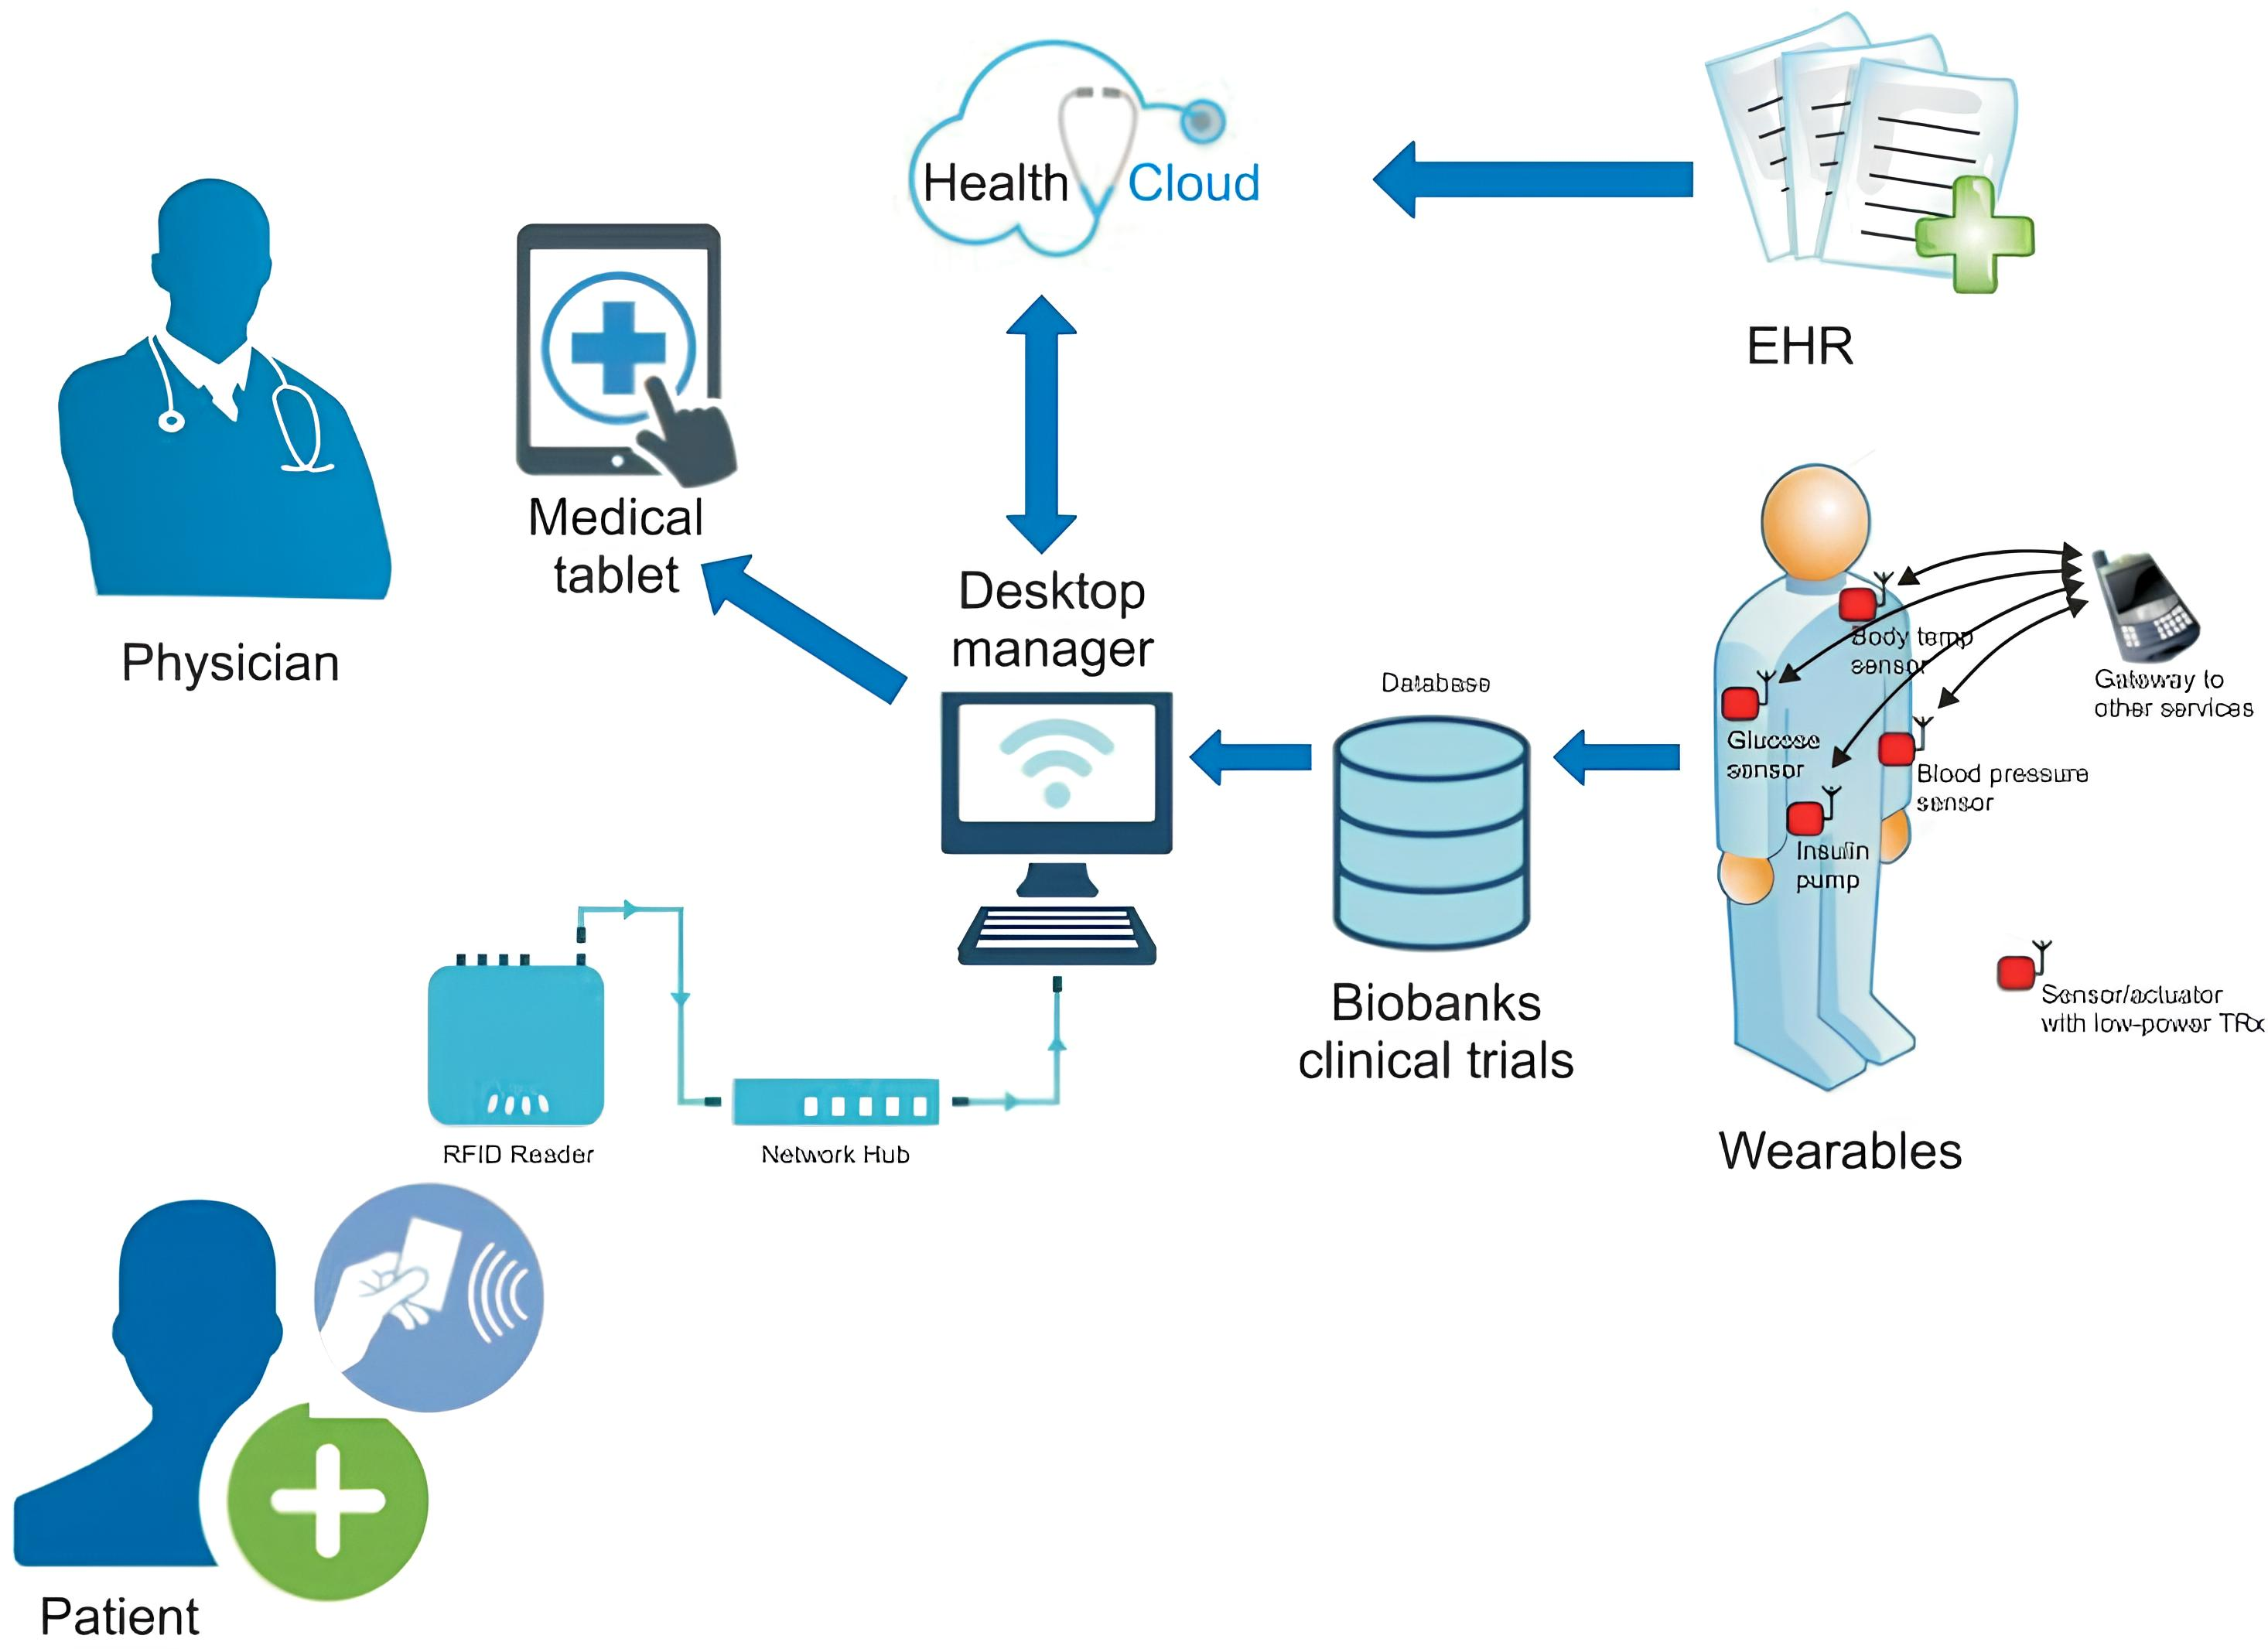
\includegraphics[width=0.6\textwidth ]{images/iot.jpg}
    \caption{Un'illustrazione di come questa rivoluzione 
    nella medicina apparirà in un tipico ospedale che fa uso di IOT}
\end{figure}\\
Le diverse tecnologie vengono incanalate in determinate linee guida di sviluppo, i sistemi distribuiti che permettono 
la circolazione rapida di informazioni sono combinati ad una centralizzazione della gestione di essi, garantendo la possibilità 
di controllare e monitorare in modo efficiente dati e risorse da e in qualsiasi parte dell'azienda.\acc Nonostante le 
macchine moderne siano indipendenti da un intervento continuo, devono essere supervisionate da un operatore umano, 
quest'ultimo deve avere la possibilità di interagire  con esse in maniera intuitiva, la branca che si occupa di rendere 
semplice tale operazione è denominata \textit{interazione uomo macchina}.
\subsection{Modelli di Business}
2 aspetti sono fondamentali nell'industria 4.0\begin{itemize}
    \item Qualità delle aziende migliorata grazie all'uso delle nuove tecnologie 
    \item Nuovi schemi di competizione del mercato basati sui nuovi modelli di business 
\end{itemize}
Tali modelli di business si sono sviluppati solo dopo l'avvento delle tecnologie abilitanti che li hanno resi 
realizzabili.\begin{itemize}
    \item \textbf{Centralità del cliente} : al centro della catena del valore dell'industria, c'è  il  consumatore, e le aziende puntano a soddisfare le richieste di quest'ultimo, talvolta anticipandone le necessità e le 
    richieste di servizio.
    \item \textbf{Economia circolare} : risponde alla necessità di passare ad un modello circolare di produzione, in 
    cui i prodotti ed i processi manifatturieri vanno improntati al riutilizzo.\begin{center}
        progetta $\longrightarrow$ usa $\longrightarrow$ ricicla $\longrightarrow$ riusa
    \end{center}
    Tale modello porta un risparmio dovuto alla riduzione degli scarti e ai minori costi di approvvigionamento, nonché 
    una notevole riduzione dell'impatto ambientale.
    \item \textbf{Strategie basate su ICT} : emergono nuove strategie di mercato che hanno lo scopo di portare il prodotto 
    più vicino al consumatore, le tecnologie alla base dell'industria 4.0 mettono a disposizione una grande mole di dati 
    utili al miglioramento dell'efficienza dell'azienda. \begin{itemize}
        \item negozi online 
        \item servizi ad abbonamento 
        \item affitto di infrastrutture informatiche 
    \end{itemize}
    \item \textbf{Economia della condivisione} : modelli di condivisione di beni e servizi tramite piattaforme digitali, come 
    i servizi di car sharing o bike sharing, irrealizzabili senza un'infrastruttura informatica, che permette il monitoraggio 
    dello stato dei veicoli.
    \item \textbf{Economia del fare} : le stampanti 3D, grazie alla prototipazione rapida, hanno permesso l'insorgere di un "artigianato digitale" 
    autoprodotto a basso costo, con uso di materiali  plasmabili e anche di robot programmati.
\end{itemize}
\subsubsection{Cloud Automation}
I robot di servizio nei centri di \textit{Amazon} che si occupano dello stoccaggio 
dei prodotti funzionano grazie a degli algoritmi di instradamento che 
ne determinano i percorsi ottimali, tali algoritmi molto spesso risultano 
costosi da un punto di vista computazionale, de facto, i robot di questo tipo 
inviano i dati ad un server centralizzato che si occupa di eseguire gli algoritmi per 
poi restituire i risultati ai robot.\acc 
Un aspetto fondamentale dell'industria 4.0 è il processo di 
\textbf{trasformazione digitale} nelle aziende tramite l'inclusione delle 
tecnologie ICT, in particolare, sono identificati 6 passi 
fondamentali nella trasformazione, che incrementano il valore 
dell'azienda e del prodotto finale.
\\\begin{figure}[h!]
    \centering
    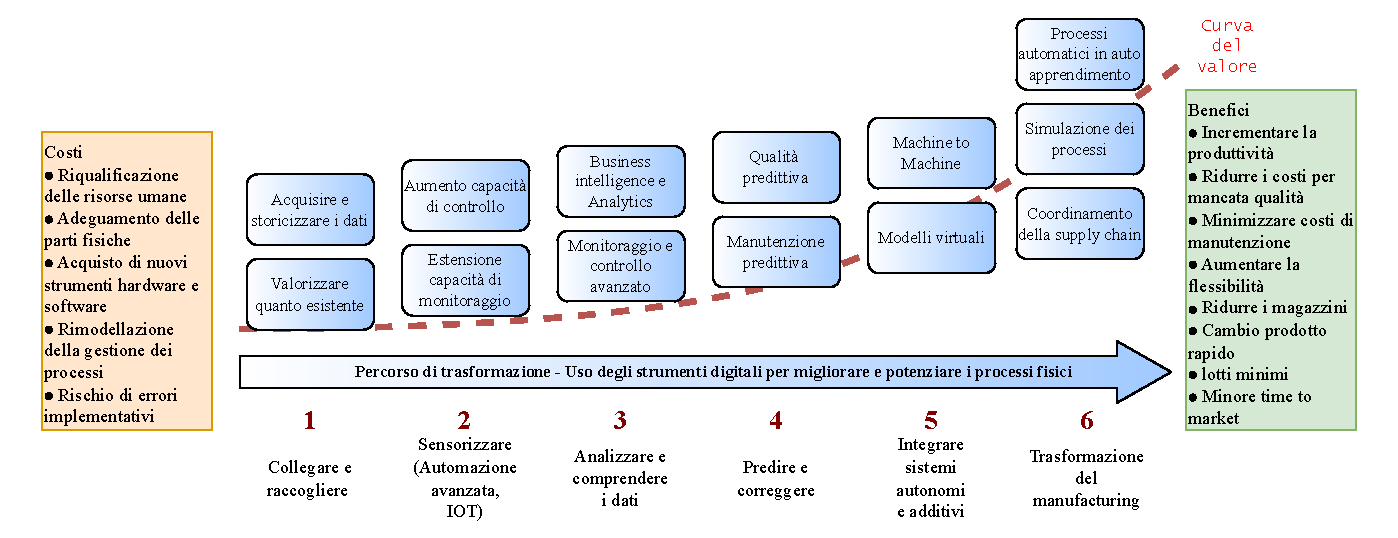
\includegraphics[width=1\textwidth ]{images/trasformazioneDigitale.pdf}
    \caption{i 6 passi della trasformazione digitale}
\end{figure}\\
 Ovviamente tale processo ha dei costi da sostenere, banalmente 
 l'implementazione di hardware e software, inoltre,è soggetto 
 ad errori che possono comportare rischi non di poco conto, i quali\begin{itemize}
    \item mancanza di una strategia chiara 
    \item mancanza di consenso ed impegno nella leadership
    \item concentrazione sulle tecnologie piuttosto che sulle persone 
    \item farsi guidare dalle tendenze senza avere una visione
    \item trascurare il contributo dei clienti
    \item voler organizzare il processo in autonomia 
    \item sottovalutare le competenze interne 
    \item non considerare la sicurezza dei dati 
    \item mancanza di flessibilità 
    \item carenza di comunicazione 
    \item sottovalutazione delle complessità
 \end{itemize}
La \textit{McKinsey} nel 2017 ha rilasciato un rapporto riguardante le attività lavorative ed il possibile 
grado di automatizzazione di queste, in particolare, si hanno i seguenti risultati, su un analisi che ha coinvolto 
circa 2000 attività lavorative relative a circa 800 occupazioni\begin{itemize}
    \item Storicamente l'automazione ha aumentato la produttività del (circa) $1\%$ all'anno
    \item Con le attuali tecnologie (in riferimento al 2017), è possibile automatizzare circa la metà delle 
    attività lavorative 
    \item Le attività che si prestano maggiormente ad essere automatizzate, son quelle che caratterizzano lavori 
    fisici, prevedibili e ripetitivi, che richiedono tipicamente basse capacità cognitive. Costituiscono circa 
    il 51\% delle attività negli USA
    \item Le occupazioni le cui attività possono essere completamente automatizzate sono circa il 5\% 
    \item Nel 60\% delle occupazioni, circa il 30\% delle attività possono essere automatizzate
    \item Il lavoro umano affiancato ai robot è necessario a garantire la crescita del PIL
\end{itemize}
\begin{figure}[h!]
    \centering
    \includegraphics[width=0.4\textwidth ]{images/andamentoLavori.eps}
    \caption{Andamento dei posti di lavoro in base al livello di educazione}
\end{figure}
\begin{center}
    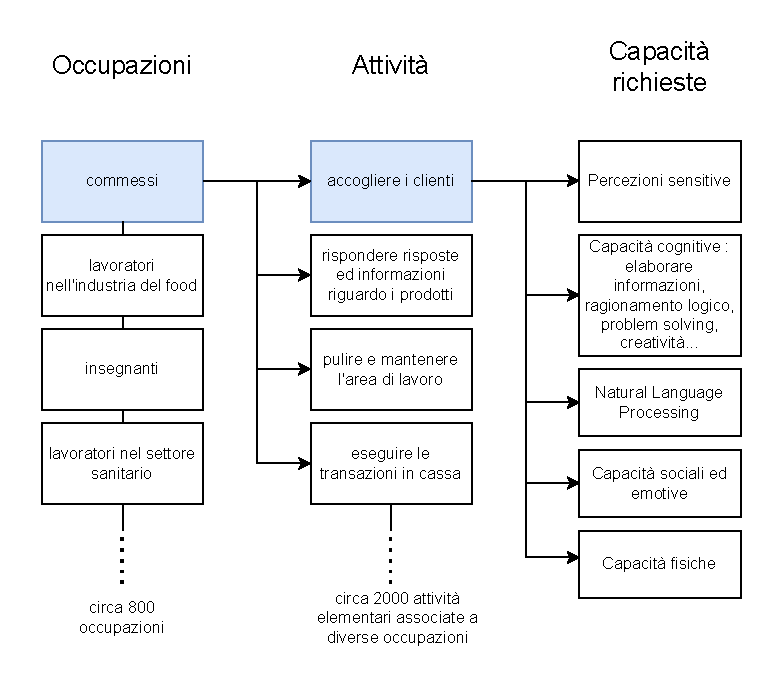
\includegraphics[width=0.8\textwidth ]{images/attivitaAutomatizzabili.pdf}
\end{center}
\subsection{Industria 5.0}
La commissione Europea ha trattato un rapporto sull'industria 5.0, che mira a sviluppare  il modello dell'industria 
4.0 verso un'industria europea sostenibile, resiliente e centrata sulla persona. Il progetto di 
ricerca \textit{Horizon Europe} punta ad investire sui progetti di ricerca che incorporano tali modelli, in Italia, 
il \textbf{PNNR} è un insieme di iniziative che puntano alla trasformazione dei sistemi di produzione, in particolare\begin{enumerate}
    \item digitalizzazione, innovazione, cultura 
    \item transazione al verde 
    \item infrastrutture per una mobilità sostenibile 
    \item istruzione e ricerca 
    \item coesione ed inclusione sociale 
    \item salute
\end{enumerate}
Come già accennato, le parole chiave dell'industria 5.0 sono le seguenti\begin{itemize}
    \item \textbf{resilienza} : gestire i cambiamenti desiderati e non (ad esempio, epidemie) con una 
    produzione  industriale
    dotata di supporti per le
    infrastrutture critiche e
    resistente a "interruzioni".
    \item \textbf{centralità della persona} : mettere l'essere umano al primo posto e chiedersi cosa 
    può fare la tecnologia per noi, e non cosa possiamo fare noi per la tecnologia, in particolare, adottarla 
    per adattare i processi produttivi alle necessità dei lavoratori.
    \item \textbf{sostenibilità} : economia circolare, riduzione dei rifiuti e dell'impatto ambientale, assicurare 
    i bisogni odierni senza mettere
    a repentaglio le future
    generazioni.
\end{itemize}



\chapter{Reti per l'Automazione}
Molti dei concetti trattati in questo capitolo, sono considerati più approfonditamente negli appunti del 
corso di 
\color{blue}\href{https://github.com/CasuFrost/University_notes/blob/main/Secondo%20Anno/Secondo%20Semestre/Reti%20di%20Elaboratori/Latex%20source%20file/Reti%20di%20Elaboratori.pdf}{Reti di Elaboratori}\color{black}.
\section{Sistemi di Comunicazione}
Le informazioni vengono condivise orizzontalmente e verticalmente 
fra i livelli della piramide CIM, in particolare\begin{itemize}
    \item si acquisiscono informazioni 
    \item si elaborano strategie 
    \item si attuano azioni correttive
\end{itemize}
I sistemi di comunicazione devono essere adeguati 
al garantire il flusso di informazioni fra i vari livelli della 
rete che differiscono nelle caratteristiche\begin{itemize}
    \item tipologie di dati differenti 
    \item differenti vincoli di comunicazione (ad es. il livello di campo 
    avrà dei vincoli real time)
\end{itemize}
È necessaria una standardizzazione dei protocolli di comunicazione digitale.
\begin{center}
    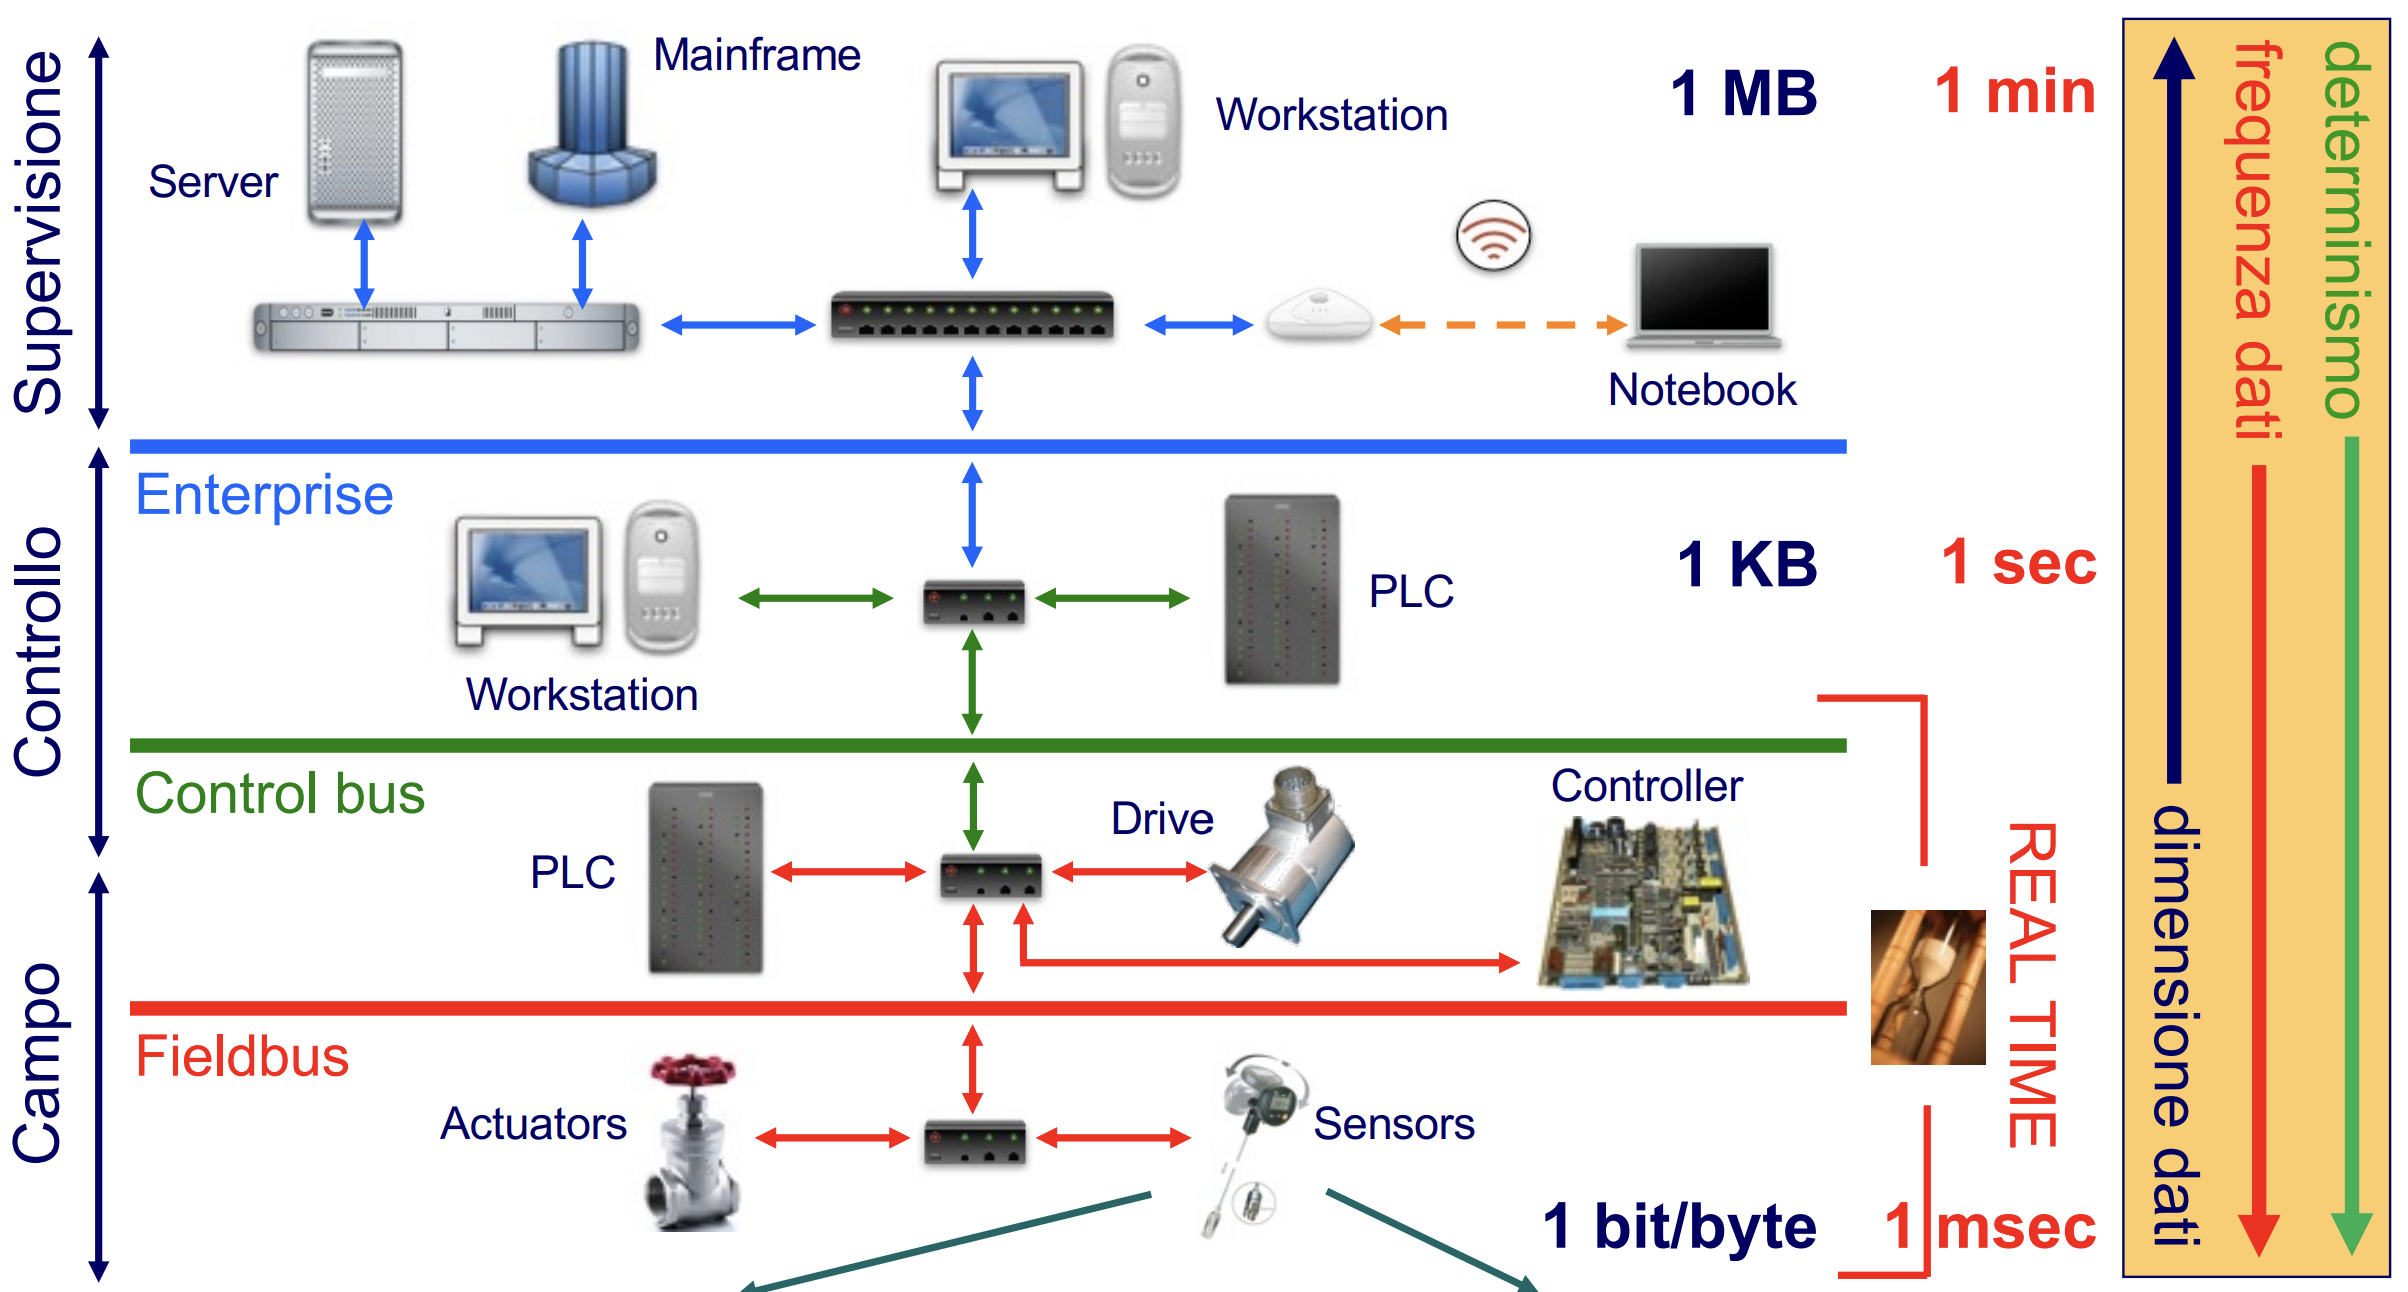
\includegraphics[width=0.8\textwidth ]{images/reti.png}
\end{center}
Gli elementi base di una rete sono \begin{itemize}
    \item Un mittente 
    \item Un destinatario 
    \item Un mezzo fisico sul quale viaggerà l'informazione 
\end{itemize}
I dati sono sul mezzo delle informazioni fisiche (luce, tensioni 
elettriche), i segnali possono essere analogici o digitali, 
in base alla definizione del protocollo. Il tipo di 
trasmissione può variare a seconda di diversi fattori, 
quali la \textbf{direzione}\begin{itemize}
    \item \textit{Simplex} : la trasmissione è unidirezionale 
    \item \textit{half duplex} : la trasmissione è bidirezionale ma 
    alternata, non si può trasmettere informazione in entrambe le direzioni 
    nello stesso momento
    \item \textit{full duplex} : bidirezionale simultanea 
\end{itemize}
il posizionamento dei bit\begin{itemize}
    \item \textit{parallela} : i bit di un byte vengono trasmessi 
    in parallelo su più canali, viene usata su distanze ridotte causa la 
    facile interferenza alla quale son soggetti.
    \item \textit{seriale} : il mezzo fisico è tipicamente 
    suddiviso in "invio","ricezione" e "massa", ed i bit di un byte 
    sono trasmessi in sequenza uno dopo l'altro. Quest'ultima può 
    a sua volta essere\begin{itemize}
        \item sincrona : i dati sono trasmessi continuamente insieme 
        ad un segnale di sincronizzazione 
        \item i dati sono trasmessi in modo irregolare a frequenza costante, 
        con bit di sincronizzazioni incapsulati nei dati 
    \end{itemize}
\end{itemize}
Le reti industriali prevedono solitamente una trasmissione digitale 
half duplex, seriale ed asincrona.\\\begin{figure}[h!]
    \centering
    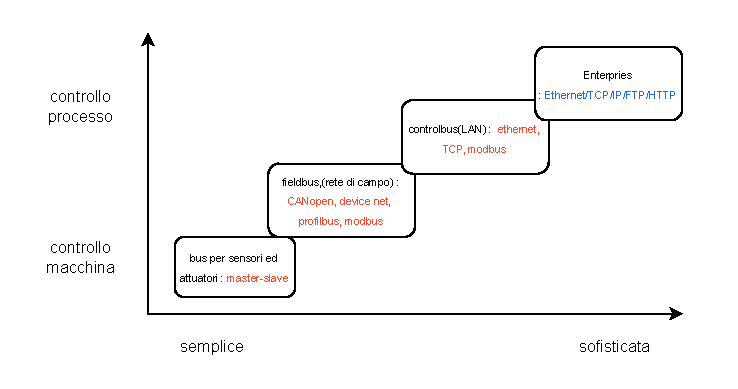
\includegraphics[width=0.85\textwidth ]{images/protocolliReti.pdf}
    \caption{tipi di reti e protocolli industriali}
\end{figure}\\
Le \textit{Rete Enterprise} sono adottate per le informazioni gestionali e seguono il classico 
modello client-server, non hanno vincoli di real-time, più che la "robustezza" dell'informazione rispetto 
ai disturbi ambientali (che possono essere presenti in una cella), è importante 
la sicurezza e la riservatezza di esse. Tali reti seguono lo standard Ethernet, e sfruttano i 
protocolli di rete e di trasporto (ossia, IP e TCP) per garantire la ritrasmissione sicura dei dati 
in caso di perdite di pacchetti.\acc 
Le reti al livello di \textit{Controllo e Campo} invece gestiscono le informazioni nelle celle 
e fra le varie macchine, i dispositivi comunicanti spesso non sono standard, ma sono PLC, controllori embedded, 
e dispositivi di campo, quindi è importante che i protocolli in tale livello siano flessibili ed 
adattabili all'eterogeneità dei client.\acc  Qui i dati trasmessi hanno piccole dimensioni, ma la 
frequenza di trasmissione è alta, e deve soddisfare i vincoli real time, per questo Ethernet non è 
appropriato e si utilizzano soluzioni apposite. Essendo l'ambiente industriale "ostile", i mezzi di 
trasmissione devono essere robusti, i ritardi nella trasmissione nella struttura ad anello dei controllori 
possono causare un degrado nelle prestazioni non trascurabile, è più che mai necessario \textit{determinismo} nella 
trasmissione.
\flowerLine 
\section{Classificazione ed Architetture delle Reti}
Nel livello di campo, esistono due possibili architetture della rete da adottare che si 
differenziano nella topologia della rete ed altri fattori. In particolare\begin{itemize}
    \item \textbf{Architettura tradizionale} : Un architettura centralizzata in cui il controllore 
    prevede un collegamento punto-punto con ogni altri dispositivo di campo.\acc 
    \textit{Vantaggi}\begin{itemize}
        \item sistema affidabile e collaudato 
        \item disponibilità di tutte le tipologie di
        strumentazione sul mercato
    \end{itemize}
    \textit{Svantaggi}\begin{itemize}
        \item elevato numero di collegamenti 
        \item cablaggio costoso 
        \item lavoro di stesura e protezione dei fili critico
    \end{itemize}
    \item \textbf{Architettura a bus di campo (fieldbus)} : Un architettura che prevede la presenza di 
    un bus centrale (la cui comunicazione è digitale)
     alla quale ogni dispositivo si connette direttamente.\acc
     \textit{Vantaggi}\begin{itemize}
        \item installazione più economica 
        \item modularità : è facile aggiungere e rimuovere dispositivi 
        \item tolleranza ai guasti 
        \item condivisione delle risorse
    \end{itemize}
    \textit{Svantaggi}\begin{itemize}
        \item i dispositivi comunicano sullo stesso mezzo, è quindi necessario un protocollo di 
        accesso al mezzo 
        \item difficile da installare in aree pericolose
    \end{itemize}
\end{itemize}\begin{figure}[h!]
    \centering
    \includegraphics[width=0.85\textwidth ]{images/tradVSfieldbus.eps}
    \caption{soluzioni a livello di campo}
\end{figure}
\subsection{Tipologie di Reti}
Una rete può essere\begin{itemize}
    \item \textbf{broadcast} : vi è un unico canale di comunicazione condiviso da ogni macchina 
    sulla rete, i messaggi arrivano ad ogni nodo, i nodi scarteranno i messaggi di cui non sono 
    destinatari. Queste possono essere a loro volta\begin{itemize}
        \item \textit{reti a bus} : canale condiviso, in ogni istante un solo nodo può trasmettere 
        contemporaneamente, è necessario arbitraggio. 
        \item \textit{reti ad anello} : i pacchetti circolano in serie su un anello, necessario 
        arbitraggio per accessi simultanei
    \end{itemize}
    \begin{center}
        \includegraphics[width=0.85\textwidth ]{images/anelloEbus.eps}
    \end{center}
    \item \textbf{peer-to-peer} : per ogni coppia di nodi vi è una connessione dedicata, 
    se due macchine non sono connesse fisicamente, è necessario definire un cammino fra di esse tramite 
    appositi algoritmi di routing, 
    se più pacchetti relativi allo stesso messaggio seguono cammini diversi, è
    necessario gestire anche la sequenza con cui essi vengono ricevuti. Vengono applicate a reti di dimensioni maggiori, normalmente 
    più reti LAN sono connnesse in tal modo.\begin{center}
        \includegraphics[width=0.85\textwidth ]{images/puntopunto.eps}
    \end{center}
    \item Nella maggioranza delle applicazioni più complesse, la soluzione più frequente 
    ricade in \textbf{reti ibride}.
\end{itemize}
Esiste una scala di classificazione delle reti :\begin{center}
    \begin{tabular}{|
            >{\columncolor[HTML]{EFEFEF}}c |
            >{\columncolor[HTML]{FFFFFF}}c |c|
            >{\columncolor[HTML]{FFFFFF}}c |}
        \hline
        \cellcolor[HTML]{9AFF99}{\color[HTML]{000000} Scala} & \cellcolor[HTML]{9AFF99}Tipo & \cellcolor[HTML]{9AFF99}Nome completo & \cellcolor[HTML]{9AFF99}Esempio \\ \hline
        Distanza ravvicinata                                 & PAN                          & Personal Area Network                 & Bluetooth                       \\ \hline
        Edificio                                             & LAN                          & Local Area Network                    & WiFi, Ethernet                  \\ \hline
        Città                                                & MAN                          & Metropolitan Area Network             & Cablata, DSL                    \\ \hline
        Paese                                                & WAN                          & Wide Area Network                     & Grandi ISP                      \\ \hline
        Pianeta                                              & Internet                     & La rete di tutte le reti              & L'Internet                      \\ \hline
    \end{tabular}
\end{center}
La \textbf{LAN} è la rete locale, come una rete domestica, è una rete privata ed ogni terminale connesso ad essa è identificato
da un indirizzo distinto dagli altri, può essere a \textit{cavo condiviso} oppure a \textit{commutazione} con uno switch.
In tale modello di cavo condiviso il pacchetto inviato ad un dispositivo viene ricevuto da tutti, solo il destinatario lo
elaborerà, tutti i restanti host lo ignoreranno.\acc
Quest'ultimo a commutazione è il più utilizzato tutt'oggi, ogni dispositivo è direttamente collegato allo switch, ed esso è
in grado di riconoscere gli host ed inviare i pacchetti esclusivamente al destinatario, riduce il traffico nella LAN.\acc
Le reti \textbf{WAN} sono reti geografiche, vengono interconnessi dispositivi di comunicazione, necessari a città, regioni o
perfino nazioni. I dispositivi in questione sono switch, router e modem, tale rete è gestita da un grande operatore/ente di
telecomunicazioni detto IPS (Internet Service Provider) che fornisce i servizi alle organizzazioni.\acc Una WAN può vedere i suoi
dispositivi di comunicazione connessi punto-punto, oppure a commutazione, con più punti di terminazione (usata nelle dorsali di
Internet), tutt'oggi è raro trovare LAN o WAN isolate, spesso sono connesse fra loro per formare una internetwork (internet), per
mettere in comunicazione due LAN in città differenti tramite una WAN.
\subsubsection{Dispositivi di Interconnessione}
Per il collegamento fra tratti di una stessa rete, oppure fra reti diverse, sono coinvolti vari dispositivi\begin{itemize}
    \item \textbf{repeater (ripetitore)} : amplifica e ricostituisce il segnale originale su segmenti analoghi della
    stessa rete [repeater RS485]
    \item   \textbf{hub (concentratore)} : estende una rete a stella, amplifica e ricostituisce lo stesso segnale su
    tutte le porte, non riduce le collisioni [Ethernet hub] 
    \item  \textbf{switch (interruttore)} : come un hub, ma su una singola porta per volta, può ridurre le
    collisioni [Ethernet switch]
    \item \textbf{transceiver (ricetrasmettitore)} : connette a una stessa rete segmenti di diversa tipologia
    [RS232/RS485 transceiver]
    \item \textbf{bridge (ponte)} : connette due reti che usano lo stesso protocollo ma che hanno layer
    differenti al livello inferiore [Modbus RS485 / Ethernet TCP-IP bridge]
    \item  \textbf{router (instradatore)} : connette due reti dello stesso tipo [Ethernet TCP-IP router] 
    \item \textbf{gateway (portale)} : connette due reti di tipo diverso [Ethernet / Modbus gateway] 
\end{itemize}
Nelle reti broadcast, l'accesso al canale può venire per vie di allocazione \begin{itemize}
    \item \textbf{statica} :  il tempo viene suddiviso in time slices (quanti) e ad ogni nodo 
    viene dedicato un intervallo periodico in cui può comunicare, nel caso non abbia nulla 
    da trasmettere, il canale resta inutilizzato (spreco di banda). 
    \item \textbf{dinamica} : Si suddivide in \begin{itemize}
        \item controllo centralizzato : un nodo \textit{master} determina il prossimo 
        dispositivo che potrà comunicare tramite strategie di polling. 
        \item controllo decentralizzato : ogni nodo decide autonomamente se trasmettere o no. 
        \item sistemi a collisione : i nodi possono trasmettere, se capita che due di essi 
        trasmettano contemporaneamente, vi sarà una \textit{collisione} che verrà 
        rilevata ed eventualmente risolta.
    \end{itemize}
\end{itemize}
\subsubsection{Architettura Software}
I 5 macro-livelli sulla quale si fonda la comunicazione sono i seguenti :
\begin{center}
    \includegraphics[width=1\textwidth ]{images/livelli.eps}
\end{center}
Sino ad ora i dati incapsulati che vengono comunicati sulla rete sono stati chiamati generalmente
"pacchetti", vedremo che questi assumono una denominazione diversa per ogni livello. Ogni protocollo
fa parte di un livello, ed anche se esistono più protocolli per un livello, ogni pacchetto
che viene trasmesso usufruisce di un solo protocollo per livello. I nomi dei protocolli citati in
seguito, verranno approfonditi e caratterizzati in seguito.
\begin{enumerate}
    \item Il livello di \textbf{applicazione} è dove risiedono le applicazioni di rete che
          usufruiscono dei servizi di Internet, alcuni dei protocolli presenti in questo livello
          sono \textit{HTTP,SMTP,FTP,DNS}, in questo livello, i pacchetti sono chiamati
          \textg{messaggi}.
    \item Il livello di \textbf{trasporto} si occupa del trasferimento dei messaggi  dal livello di
          applicazione di un client al livello di applicazione del server, alcuni protocolli sono
          \textit{TCP} e \textit{UDP}, in questo livello, i pacchetti sono chiamati
          \textg{segmenti}.
    \item Il livello di \textbf{rete} riguarda l'instradamento dei segmenti dall'origine alla
          destinazione, un noto protocollo è l'\textit{IP}, i pacchetti in questo livello sono detti
          \textg{datagrammi}.
    \item Il livello di \textbf{collegamento} si occupa della trasmissione dei datagrammi da un
          nodo della rete al nodo successivo sul percorso, alcuni protocolli sono \textit{Ethernet,Wi-Fi e
              PPP}, lungo un percorso sorgente-destinazione, un datagramma può essere gestito anche da
          differenti protocolli, i pacchetti qui sono detti \textg{frame}.
    \item Il livello \textbf{fisico} riguarda il trasferimento dei singoli \textbf{bit} sul canale
          fisico, tramite elettricità nei cavi, oppure onde elettromagnetiche.
\end{enumerate}
Durante la comunicazione, non tutti i sistemi intermedi richiedono che il messaggio venga processato
su tutti i livelli, alcuni dispositivi richiedono solo alcuni layer, riducendo la complessità.
\begin{center}
    \includegraphics[width=1\textwidth ]{images/comunicazioneProtocolli.eps}
\end{center}
Lo strato di un livello ha una comunicazione logica/virtuale con lo stesso livello su un altro
computer, ma i dati non sono trasferiti direttamente da uno strato all'altro, passano per tutti i livelli
inferiori, un \textit{protocollo} è quindi un insieme di regole che controllano il formato ed il
significato dei pacchetti scambiati tra le entità \textit{pari} all'interno di uno strato, un
\textit{servizio} invece è un insieme di primitive che uno strato offre a quello superiore, ossia :\begin{itemize}
    \item Quali operazioni fornisce (senza dire nulla sull'implementazione).
    \item Posto come interfaccia fra due strati, quello inferiore fornisce il servizio, quello superiore ne
          usufruisce.
\end{itemize}\flowerLine
\section{Livello Fisico e di Collegamento}
Il livello fisico dello stack protocollare riguarda la trasmissione fisica dei bit sul canale e la definizione delle convenzioni elettriche. Esistono differenti mezzi di trasmissione dei dati\begin{itemize}
    \item \textit{doppino telefonico} : È una coppia di cavi intrecciati, mezzo piuttosto antiquato e la trasmissione è nell'ordine dei Kbps (Kilobit per secondo).
    \item \textit{cavo coassiale} : È un conduttore di rame circondato da materiale isolante, resiste bene ai disturbi e la banda è buona, la trasmissione è nell'ordine dei Mbps. 
    \item \textit{fibra ottica} : È un cavo in fibra di vetro in cui l'informazione passa sotto forma di impulsi luminosi. I segmenti possono essere lunghi fino a 2km e la trasmissione è nell'ordine dei Tbps.
    \item \textit{wireless} : La trasmissione si propaga nel vuoto sotto forma di onde elettromagnetiche.
\end{itemize}
\begin{center}
    \includegraphics[width=0.75\textwidth ]{images/cavoCoassiale.pdf}
\end{center}
L'informazione viene codificata con dei bit che vengono trasmessi su diversi spettri di sequenza, con media del segnale nulla oppure no. Una codifica ideale ricerca\begin{itemize}
    \item mantenimento sincronizzazione sorgente/destinazione
    \item bassa probabilità di errore (a causa di rumore/interferenze)
    \item minima banda utilizzata, a parità di informazione trasmessa
    \item capacità di rivelazione di errori
\end{itemize}

La \textbf{codifica binaria diretta} più semplice, dove un livello alto di tensione rappresenta un 1 e un livello basso (o assenza di segnale) rappresenta uno 0, si dice non polare quando l'assenza di segnale rappresenta un bit, è polare invece quando l'assenza di segnale è associata alla non trasmissione.
\begin{center}
    \includegraphics[width=0.75\textwidth ]{images/codBinPol.eps}
\end{center}
La codifica \textbf{return to zero (RZ)} prevede il ritorno del segnale a zero volt almeno una volta per ogni bit trasmesso, permettendo di inserire un riferimento temporale per la sincronizzazione dei dati. Saranno quindi utilizzati due clock, uno legato alla frequenza dei bit (indica l'inizio e fine di ogni bit), ed un altro con 
frequenza doppia rispetto al  primo clock, viene utilizzato per individuare il punto medio di ogni bit, ovvero il momento esatto in cui il segnale ritorna a zero.
\begin{center}
    \includegraphics[width=0.75\textwidth ]{images/RZ.eps}
\end{center}
Nella codifica \textbf{manchester}, simile a quella RZ, il clock viene utilizzato per metà, la prima parte viene utilizzata per l'informazione, la seconda per una "risalita" o "discesa" verso lo zero, cambiando bit.
\acc La codifica \textbf{manchester differenziale} è simile alla codifica manchester ma il segnale viene paragonato con il semiperiodo precedente per far si che ci sia sempre un cambio di segnale al "centro" del bit time.
l'assenza di transizione al centro del bit time indica una violazione
della codifica: viene usata per delimitare un frame di trasmissione.
\begin{center}
    \includegraphics[width=0.7\textwidth ]{images/manchester.eps}
\end{center}
Esistono differenti standard di connessione elettrica/meccanica:\begin{itemize}
    \item IEEE RS232  :(tra i più consolidati, punto-punto),
     comprende un connettore a 25 pin la trasmissione è limitata a  20Kbps e la lunghezza dei segmenti è al più di 15 metri.
     \item IEEE RS422 : ampiamente utilizzato in ambito industriale, il troughput è fino a 10Mbps ed i segmenti possono essere lunghi anche 1200 metri.In configurazione simplex, la comunicazione avviene in una sola direzione, può essere composto da due coppie di cavi più massa per il full duplex.\acc In una rete connessa in tal modo ci può essere al più un trasmettitore alla volta e al più 10 ricevitori.\acc 
     Il segnale viene trasmesso in modo differenziale, ovvero come la differenza tra due segnali complementari (A e -A). Questo metodo permette di ridurre notevolmente il rumore e aumenta la distanza di trasmissione.
     \item IEEE RS485 : anch'esso ampiamente adoperato in ambito industriale, 
    utilizza la trasmissione differenziale e offre una buona immunità ai disturbi. A differenza dell'RS422, l'RS485 è half-duplex, ovvero la comunicazione avviene in una sola direzione alla volta.\acc 
    RIsulta necessario controllare l'accesso, solo un dispositivo può trasmettere alla volta. Gli altri dispositivi hanno il circuito di ingresso in uno stato di alta impedenza, come se fossero scollegati. Questo meccanismo evita conflitti durante la trasmissione.
\end{itemize}\begin{figure}[h!]
\centering
\includegraphics[width=0.4 \textwidth ]{images/RS485.eps}
    \caption{RS485}
\end{figure}
\subsection{Protocolli MAC}
Il livello di collegamento si occupa di ricevere i dati da inviare e di suddividerli in \textit{frame}. Si occupa anche di inviare appositi ACK (messaggi di conferma di ricezione) per la comunicazione affidabile e di gestire \textbf{l'accesso al mezzo fisico (MAC)}.\acc 
Il \textbf{CSMA/CD} (Carrier Sense Multiple Access / Collision Detection) è un protocollo per l'accesso al mezzo in cui i nodi sono costantemente in ascolto sul canale, quando un nodo trasmette, confronterà il segnale di ritorno con il segnale originale, se differiscono, vorrà dire che c'è stata una collisione. Ogni nodo a seguito di una collisione attenderà un lasso di tempo casuale prima di ritrasmettere.\acc 
Nel \textbf{CSMA/CR}   (Carrier Sense Multiple Access / Collision Resolution) ogni nodo è sempre in ascolto sul canale, è il metodo MAC utilizzato nei protocolli \textit{CAN} e \textit{CANOpen}, vi è uno stato fisico del canale che si occupa dell'\textit{arbitraggio logico} a livello dei bit.
Ogni dispositivo ha un identificativo (ID) unico, codificato in una sequenza di bit. Quando un dispositivo vuole trasmettere, trasmette il suo ID bit per bit sul bus.\begin{itemize}
    \item Se più dispositivi trasmettono contemporaneamente, si verifica una collisione.
    \item Il bus calcola l'AND bit a bit degli ID dei dispositivi che stanno trasmettendo.
    \item Il dispositivo che ha trasmesso il bit dominante (solitamente 0) in quella posizione dell'ID "vince" la collisione e continua a trasmettere il bit successivo.
    \item Gli altri dispositivi che hanno perso la collisione interrompono la trasmissione e riprovano più tardi.
\end{itemize}\begin{center}
    \includegraphics[width=0.5 \textwidth ]{images/collisionRes.eps}
\end{center}
Il modello \textbf{Token Bus/Ring} vede i nodi della rete scambiarsi un "token", uno speciale pacchetto di dati che regola i turni di trasmissione. Al costo di aumentare la latenza di trasmissione, si eliminano le collisioni.\acc 
Precisamente, quando un nodo vuole trasmettere ed è in possesso del token\begin{itemize}
    \item  lo modifica e
    rispedisce in circolo assieme al frame del dato (e con un host destinatario)
    \item " la presenza del token “modificato” non permette la trasmissione agli altri nodi
    \item il ritorno del token modificato al nodo trasmettente indica l'avvenuto successo della trasmissione \item il
    token originale viene rimesso in circolo e altri nodi potranno quindi trasmettere
\end{itemize}
L'utilizzo di differenti token permette un partizionamento dei messaggi per livelli di priorità.\flowerLine 
\section{I Protocolli Fieldbus}
Nell'ambito dell'automazione lo stack protocollare viene ridotto considerando esclusivamente \begin{itemize}
    \item livello di applicazione (tipo di comunicazione)
    \item livello di collegamento (gestione dell'accesso)
    \item livello fisico
\end{itemize}
Le reti field bus vedono diversi nodi, detti \textit{DLE} (Data Link Element), collegati ad una comune rete elettrica dove viaggia l'informazione. Vi è un elemento speciale, il \textbf{Link Active Scheduler (LAS)} che si occupa di gestire staticamente l'accesso al mezzo concedendolo ai vari DLE tramite un'apposita tabella di scheduling, l'esecuzione dei task periodici real time. Negli intervalli di tempo liberi non occupati dai task periodici, vengono gestiti i task periodici in modo dinamico.\acc 
Il LAS utilizza un token per la concessione ai DLE dell'utilizzo del mezzo, questi ultimi una volta finito, dovranno restituire un frame \textit{return token} in modo che il LAS possa passare al prossimo DLE. Le reti fieldbus sono caratterizzate da \begin{itemize}
    \item mezzo fisico : doppino twisted schermato (2 fili o 4 fili)
    \item rete a bus con brevi tratti e resistenze di 120$\Omega$ come terminatori di linea. 
    \item caratteristiche del mezzo\begin{itemize}
        \item massima lunghezza: 1000 m
        \item 9 velocità: da 10Kbps a 1 Mbps, in funzione della lunghezza del bus (1 Mbps @25 m)
        \item massimo numero di dispositivi: 128 (1 master e 127 slaves)
        \item vari tipi di connettori: RJ45, 9-pin SUB D DIN 41652, ecc...
    \end{itemize}
    \item protocolli di accesso al mezzo fisico : CSMA/CR oppure CSMA/CA\begin{itemize}
        \item ogni dispositivo può inviare dati appena il bus è libero
        \item arbitraggio delle collisioni non-distruttivo a livello di bit, con bit 0 dominante
        \item messaggi a priorità maggiore hanno valore binario minore dell'identificatore
    \end{itemize}
    \item il modello della comunicazione è \textit{producer/consumer}\begin{itemize}
        \item formato frame: 11 bit in testa indicano tipo dei dati utili trasmessi e nodo produttore
        \item seguono 5 bit di controllo (RTR, start, lunghezza dati)
        \item seguono i dati utili: massimo 8 bytes per frame
        \item dispositivi e procedure a elevata sicurezza
    \end{itemize}
\end{itemize}





\chapter{Sistemi di Controllo Real Time}
Nell'ambito dell'automazione, è fondamentale definire un sistema di controllo che agisca in tempo reale, che 
implementi un algoritmo con lo scopo di eseguire i generici task di un processo produttivo, lo scopo dell'algoritmo 
è quello di \textit{sequenziare} le varie operazioni in modo che rispettino dei vincoli temporali.\acc 
In un processo vi è un insieme diffusi di singoli componenti (come sensori o attuatori) che comunicano con il 
sistema di controllo che gestisce i riferimenti dei segnali, i valori di riferimento sono determinati 
dall'\textit{algoritmo} in questione, che viene implementato attraverso gli strumenti dell'informatica.\begin{center}
    \includegraphics[width=0.8\textwidth ]{images/algoritmoControllo.pdf}
\end{center}
L'algoritmo si definisce \textbf{logicamente corretto} se, definiti i dati in ingresso ed i dati in uscita, fornisce i 
risultati attesi. Si dice \textbf{temporalmente corretto} se i risultati forniti rispettano i vincoli di tempo (deadline) 
imposti. Un sistema \textit{real time} deve essere logicamente e temporalmente corretto.\acc 
Erroneamente, si può pensare che per far si che un sistema sia real time (rispetti i vincoli di tempo), basti 
rendere il sistema più veloce aumentando la potenza di calcolo, ciò non è in realtà sufficiente, è necessario 
che l'unità di calcolo si dedichi esclusivamente all'algoritmo di controllo, è quindi importante che sia 
correttamente configurato. \acc 
Un sistema deputato al real time deve dare \textit{massima priorità} all'algoritmo di controllo, per questo i 
sistemi real time sono sistemi dedicati realizzati ad hoc, e non vengono utilizzati i sistemi come 
windows o linux, in quanto essendo general purpose, prevedono molte funzionalità (ad esempio, la gestione dell'I/O) che 
possono ritardare l'esecuzione dell'algoritmo.\acc 
Un sistema real time deve quindi essere \textit{prevedibile} e \textit{deterministico}, possiamo suddividere 
i task da sequenziare in due categorie \begin{itemize}
    \item relativi alla sicurezza 
    \item nice to have
\end{itemize}
I task responsabili (direttamente o indirettamente) della sicurezza fisica delle persone devono avere 
massima priorità e la loro esecuzione deve essere strettamente deterministica, un esempio di task di questo tipo, 
è l'azionamento del freno di un ascensore. I task nice to have invece, "prenotano" l'esecuzione ma potrebbero 
dover dare la priorità ai task più importanti, un esempio di task di questo tipo può essere l'attivazione 
dello stereo in un automobile (nice to have = godibile, ma non fondamentale).\acc 
Introduciamo a tal proposito due coefficienti, siano \begin{itemize}
    \item $r_c$ : risultati corretti 
    \item $r_e$ : risultati elaborati 
    \item $r_t$ : risultati ottenuti rispettando i vincoli \end{itemize}Si hanno\begin{itemize}
    \item \textbf{coefficiente logico} : $C_l=\dfrac{r_c}{r_e}$
    \item  \textbf{coefficiente temporale} : $C_t=\dfrac{r_t}{r_e}$
\end{itemize}
Un sistema si dice \textbf{hard real time} se entrambi i coefficienti sono uguali ad 1. I già accennati task 
che hanno a che fare con l'incolumità delle persone devono essere hard real time. I sistemi \textbf{soft real time} 
garantiscono la correttezza temporale solamente per una certa percentuale di task. 
\begin{itemize}
    \item hard real time  : $\min(C_l,C_t)=1$ 
    \item soft real time :  $\min(C_l,C_t)<1$
\end{itemize}
Per un generico task denotiamo $T_i$ il tempo minimo necessario per eseguirlo, e denotiamo $d_i$ la 
sua deadline (tempo massimo in cui va eseguito), il \textit{vincolo real time} $\nicefrac{T_i}{d_i}$
da una misura sul margine di tempo rimanente fra il completamento di un task e la sua deadline, deve essere 
auspicabilmente minore di 1. Se è molto minore di 1, si dice che il vincolo è \textit{largo}, se è prossimo all'unità, 
allora è \textit{stretto} ed implica una programmazione sistematica.\flowerLine 
\section{Parallelismo e Programmazione Concorrente}
I task verranno rappresentati tramite un diagramma che prevede un asse temporale e dei blocchi 
rappresentanti la "vita" di tali task nel tempo.
\begin{center}
    \includegraphics[width=0.7\textwidth ]{images/diagrammaTask.eps}
\end{center}
Un \textit{evento} avviene in un certo istante di tempo e sancisce il momento in cui il task 
può cominciare, tale diagramma individua l'intervallo temporale in cui il task è pronto per 
essere eseguito fino al momento in cui deve essere terminato. Può accadere che i timescope di due task si 
intersechino necessitando di un esecuzione \textit{parallela}.\begin{center}
    \includegraphics[width=0.7\textwidth ]{images/diagrammaTaskParalleli.eps}
\end{center}
Un sistema di controllo con $n$ processori permette il \textit{parallelismo reale}, in cui 
nello stesso istante più task vengono eseguiti in parallelo su differenti unità di calcolo. Dato che in genere, il numero dei task 
è sempre maggiore del numero dei processori, è necessaria la gestione del \textbf{parallelismo logico}, in cui più 
task vanno alternati su un singolo processore, varrà quindi l'ipotesi che l'unità di calcolo dei sistemi di controllo 
trattati in questo corso sia unica.\acc 
L'obiettivo è quello di disegnare un \textbf{algoritmo di scheduling}, che si occupi di decidere in che modo i 
task vanno sequenziati nel tempo. Molti dei concetti presenti sono ampiamente trattati negli appunti del corso di 
\color{blue}\href{https://github.com/CasuFrost/University_notes/blob/main/Secondo%20Anno/Primo%20Semestre/Sistemi%20Operativi%201/Latex%20source%20file/Sistemi%20Operativi%20modulo%201.pdf}{Sistemi Operativi 1}.\color{black}
\subsubsection{Caratteristiche di un Task}
Ogni task nell'ambiente del sistema di controllo, in un preciso istante può trovarsi in uno dei seguenti stati\begin{itemize}
    \item \textit{attivo} : L'evento che lo ha scaturito è precedente all'istante attuale, e la sua deadline è futura 
    all'istante attuale. Un task attivo inoltre può essere \begin{itemize}
        \item \textit{pronto} : attivo, ma in attesa di essere eseguito sul processore. 
        \item \textit{in esecuzione} : in esecuzione sul processore.
    \end{itemize} 
    \item \textit{Inattivo} : Il contrario di attivo.
\end{itemize}
Inoltre per ogni task $i$ sono definiti i seguenti istanti che lo caratterizzano \begin{itemize}
    \item \textit{activation time}  $a_i$ : L'istante in cui avviene l'evento che lo scaturisce. 
    \item \textit{start time} $s_i$ : L'istante in cui viene eseguito sul processore per la prima volta. 
    \item \textit{end time} $e_i$ : L'istante in cui l'esecuzione è terminata. 
    \item \textit{deadline} $d_i$ : L'istante in cui la vita del processo non può protrarsi oltre.
    Inoltre, dati gli istanti presentati, si identificano 4 intervalli di tempo relativi ad un task $i$ :\begin{itemize}
        \item \textit{computation time}  $C_i = e_i-s_i$ : il tempo effettivo impiegato sul processore.  
        \item \textit{deadline relativa} $D_i=d_i-a_i$ : la durata del suo timescope.  
        \item \textit{response time} $R_i = e_i-a_i$ : tempo impiegato per completare il task.  
        \item \textit{lateness} $L_i=e_i-d_i$ : il ritardo fra la deadline e la terminazione del processo, se 
        tale valore è maggiore di 0 si parla di soft real time, deve auspicabilmente essere minore di 0. 
    \end{itemize}
\end{itemize}\begin{center}
    \includegraphics[width=0.9\textwidth ]{images/istantiDelTask.eps}
\end{center}
Lo scheduler (unità logica che applica l'algoritmo di scheduling) deve attuare una strategia che \begin{itemize}
    \item Rispetti i vincoli delle risorse 
    \item Rispetti le priorità dei task 
    \item Massimizzi opportuni indici prestazionali 
\end{itemize}
Quando un evento genera un task, questo viene messo nella \textit{ready queue}, ossia la coda 
dei task pronti per essere eseguiti, l'algoritmo deve selezionare dalla coda il task successivo che 
verrà eseguito sull'unità di calcolo (dispatching), inoltre uno scheduler può essere \textbf{preemptive} : \begin{quote}
    Se vi è un processo $A$ in esecuzione e ne arriva nella ready queue uno nuovo $B$ di priorità maggiore, lo scheduler 
    \textit{ preemptive} bloccherà l'esecuzione del processo $A$ per eseguire il processo $B$, una volta terminato, $A$ 
    potrà tornare in esecuzione.
\end{quote}
I task, possono richiedere l'accesso a delle risorse \begin{quote}
    Ad esempio, un task che si occupa della stampa di un foglio può richiedere accesso alla stampante
\end{quote}
Inoltre queste risorse possono essere condivise fra più task, l'accesso a queste deve essere \textbf{mutualmente 
esclusivo}, quando un task sta utilizzando una risorsa, nessun task che la necessita può essere eseguito. 
I task pronti ad essere eseguiti, ma che richiedono una risorsa già in uso, vengono messi in una 
\textit{blocked queue}, e saranno "bloccati" finché la risorsa di cui necessitano non tornerà disponibile.\begin{center}
   \begin{figure}[h!]
    \centering
    \includegraphics[width=1\textwidth ]{images/scheduler.pdf}
    \caption{modello generico di scheduling}
   \end{figure}
\end{center}
\flowerLine 
\section{Il Problema dello Scheduling}
Lo scheduling viene applicato a livello di coordinamento per la sequenziazione dei task, 
in particolare, il problema consiste nel sequenziare $n$ task, a cui sono associati i rispettivi 
vincoli temporali e di accesso alle risorse, ci si impone una percentuale $\pi$ di task che 
rispettino la correttezza temporale, e che eventualmente rispettino i vincoli di mutua 
esclusione nell'accesso alle risorse.\acc 
\defi{} Dato un insieme di task, esso è \textit{schedulabile} se esiste almeno un algoritmo 
di scheduling che lo \textit{risolve} (ne trova una sequenziazione ammissibile, ossia che 
rispetti i vincoli).\acc s
Si consideri il seguente esempio, vi sono due task $(A_1,A_2)$, con i rispettivi vincoli 
temporali
$$\begin{matrix}
    a_1=35 & C_1=55 & D_1=80&d_1=115\\ 
    a_2=10 & C_2=60 & D_2=145&d_2=155
\end{matrix}$$
Il tempo è misurato in generiche unità di tempo $t.u.$. Per lo scheduling di questi task, si tenta un 
approccio \textbf{First In First Out (FIFO)}, ossia, si schedulano i task in ordine di 
arrivo.\begin{center}
    \includegraphics[width=1\textwidth ]{images/esempioFIFO.eps}
\end{center}
Come si vede dalla traccia dello scheduling, l'algoritmo FIFO non risolve il problema in quanto fa 
si che il task $A_1$ termini all'istante $125$ nonostante la sua dead line assoluta fosse $115$. Si prova 
allora uno scheduling FIFO ma di tipo preemptive, in cui si da priorità al task con tempo di completamento 
minore.\begin{center}
    \includegraphics[width=1\textwidth ]{images/esempioFIFOPreemptive.eps}
\end{center}
Questa serializzazione dei task è ammissibile dato che i vincoli temporali sono rispettati, l'algoritmo 
FIFO Preemptive risolve l'insieme $(A_1,A_2)$.\acc 
Ci si pone la domanda : Esiste un algoritmo generale che, dato un arbitrario numero di task con 
rispettivi vincoli temporali, ne trovi una serializzazione ammissibile? Si è dimostrato che il problema 
dello scheduling è NP-completo, non è possibile trovare una soluzione in maniera efficiente. Nell'ambito dell'automazione 
industriale però, è possibile concedersi ipotesi largamente semplificate che permettono di 
adoperare degli algoritmi che risolvano gli insiemi di task trattati in tali contesti.
\subsection{Classificazione degli Algoritmi}
Gli algoritmi di scheduling si classificano secondo 5 differenti parametri. Un algoritmo può essere\begin{itemize}
    \item \textbf{best effort} : non è hard real time, $\pi<1$
    \item \textbf{guaranteed} : è hard real time, $\pi=1$, rispetta sempre i vincoli temporali, per garantire 
    la correttezza si basa su alcuni "test" di garanzia, quando evento genera un task, vi è una fase di 
    \textit{admission control} in cui il task viene accettato nella ready queue solo se, la sua aggiunta 
    all'insieme dei task lo rende ancora un insieme schedulabile.\begin{center}
        \includegraphics[width=1\textwidth ]{images/admissionControl.pdf}
    \end{center}
\end{itemize}
Un altro criterio di classificazione è il seguente, uno algoritmo può essere\begin{itemize}
    \item \textbf{mono processore} (verranno trattati questi)
    \item \textbf{multi processore}
\end{itemize}
Può essere inoltre \begin{itemize}
    \item \textbf{preemptive} : se esso è in grado di interrompere l'esecuzione in una delle unità di
    calcolo di un task a minor priorità a favore dell'esecuzione di un task a maggior
    priorità.
    \item \textbf{non preemptive} :  se esso non è in grado di interrompere l'esecuzione di un task
    quando esso è stato inviato ad una delle unità di calcolo.
\end{itemize}
Un importante distinzione è la seguente\begin{itemize}
    \item \textbf{offline} : Se le decisioni di scheduling sono prese prima dell'attivazione dei task, 
    quindi la sequenza è nota a priori. 
    \item \textbf{online} : Se le decisioni dipendono dall'ordine di arrivo dei task. 
\end{itemize}
L'algoritmo FIFO è online perché le decisioni dipendono dagli activation time. L'ultima distinzione 
è la seguente\begin{itemize}
    \item \textbf{dinamico} :  I parametri sulla quale si basa il dispatching (priorità) possono 
    variare nel tempo.
    \item \textbf{statico} : I parametri sulla quale si basa il dispatching (priorità) sono costanti.
\end{itemize}
FIFO è un algoritmo statico che basa le priorità sull'activation time.\acc 
\prop{}  Un algoritmo offline è anche necessariamente statico. \acc
\dimo{}  Supponiamo per assurdo che un algoritmo offline sia dinamico, ad un certo istante 
$t$, un generico evento $E$ comporta un cambio nei parametri su cui si basa lo scheduling, 
facendo cambiare l'ordine di serializzazione, tale ordine non era però noto a priori in quanto è 
dipeso dall'evento $E$, quindi è impossibile che l'algoritmo sia offline.\begin{center}
    \includegraphics[width=1\textwidth ]{images/diagrammaSinottico.pdf}
\end{center}
In generale, gli algoritmi guaranteed sono dinamici e online (hanno più gradi di libertà), ma sono anche 
computazionalmente più  complessi.
\subsection{Scheduling di Task Periodici}
Nel controllo dell'automazione industriale, i task presentano delle proprietà comuni, è possibile 
identificare nel processo produttivo dei \textit{cicli di lavoro} che si ripetono periodicamente. L'ipotesi 
di periodicità che a breve verrà definita, ha notevole impatto sulla risoluzione dei task. 
Come prima ipotesi, si assume che vi è un insieme finito di $n$ task, che possono ripetersi nel tempo, 
ossia possono esistere più istanze dello stesso task in istanti diversi, il generico task $A_i$ verrà 
ora denotato $A_i^k$, dove $k$ rappresenta la sua $k$-esima apparizione. Anche i parametri già definiti 
dipenderanno da $k$ 
$$ \begin{matrix}
    \text{parametri}&&&\text{intervalli}\\
    a_i(k) & & & C_i(k) \\ 
    s_i(k) && & D_i(k)\\
    e_i(k)&& & R_i(k)\\ 
    d_i(k)&& &L_i(k)
\end{matrix}$$
\textbf{Osservazione} : Quando si tratta il computation time, si intende sempre il tempo di lavoro minimo 
possibile per completare un task. La riduzione del computation time di un task rappresenta nel mondo reale 
l'utilizzo di una strumentazione differente capace di eseguire lo stesso task in tempo minore. D'altro canto, 
l'aumento del computation time rappresenta l'acquisto di una strumentazione \textit{più economica} 
che esegue lo stesso task in tempo maggiore.\acc
\defi{} Dato un task $A_i$ di un insieme di task, si definisce \textbf{activation period} (oppure 
periodo di attivazione) il valore (in funzione della $k$-esima occorrenza) : 
$$ T_i(k)=a_i(k+1)-a_i(k)$$ 
rappresenta il periodo che intercorre fra la $k$-esima attivazione di un task e la sua $k+1$-esima 
attivazione. Diremo che il task $A_i$ è \textbf{periodico} se per ogni $k$, l'activation period è 
costante \eqImportante{$T_i(k)=T_i(k+1) \ \ \ \ \forall k\in\N$}
Vuol dire che il task si ripete periodicamente scandito da un certo periodo.\begin{center}
    \includegraphics[width=1\textwidth ]{images/taskPeriodico.eps}
\end{center}
Inoltre, verranno formulate \textit{ulteriori ipotesi} che da questo punto in poi devono considerarsi vere 
nell'ambito dei task periodici.\begin{enumerate}
    \item La deadline relativa di un task periodico sarà uguale al suo periodo di attivazione.
    \item I task sono fra loro indipendenti (non ci sono blocking queue)
    \item Il computation time $C_i$ di un task è costante per tutte le sue istanze 
    \item Tutti i task condividono il primo activation time : $\forall i,j\in[1\dots, n] \ \ a_j(1)=a_i(1)$
\end{enumerate}
Definiamo adesso i parametri in gioco quando si tratta dello scheduling di task periodici. Il generico problema 
di scheduling prevede \begin{itemize}
    \item Un insieme di $n$ task periodici $(A_1,A_2,A_3\dots,A_n)$ 
    \item I \textit{Requisiti}, ossia i periodi di attivazione per ogni task $(T_1,T_2,T_3\dots,T_n)$
    \item I \textit{Vincoli}, ossia i computation time per ogni task $(C_1,C_2,C_3\dots,C_n)$
\end{itemize}
\defi{} Dato un insieme di $n$ task periodici con rispettivi requisiti e vincoli, si definisce 
\textbf{fattore di utilizzazione} il coefficiente $$ 
U=\sum_{i=1}^n\frac{C_i}{T_i}
$$
Il denominatore di $U$, ossia il minimo comune multiplo dei periodi 
$$ \mcm(T_1,T_2\dots,T_n)$$
rappresenta il \textit{periodo totale del sistema}, ossia il periodo con cui l'intero insieme 
di task si ripete ciclicamente. È quindi opportuno restringere lo scheduling solo per le 
prime $\mcm(T_1,T_2\dots,T_n)$ unità di tempo, in quanto per le successive sarà semplicemente 
una ripetizione di queste. Il numeratore di $U$ invece rappresenta le unità di tempo in cui 
il processore è effettivamente utilizzato.\acc 
Dato un problema di scheduling, la \textbf{condizione necessaria} affinché sia risolvibile è che 
il fattore di utilizzazione sia minore o uguale ad 1. $$ \begin{cases}
    U\le 1 \text{ possibilmente risolvibile }\\ 
    U>1 \text{ non risolvibile}
\end{cases}$$
Si prenda in esempio la coppia di task $$ 
\begin{matrix}
    A_1 & & & T_1=8 & & & C_1 =2\\ 
    A_2 & & & T_2=12 & & & C_2=8
\end{matrix}
$$
Si ha 
$$ U=\frac{2}{8}+\frac{8}{12}=\frac{22}{24}\simeq 0.917 < 1$$
L'insieme potrebbe essere schedulabile. Verrà applicato un algoritmo preemptive che 
assegna maggiore priorità al task il cui activation period è minore. Verrà quindi sempre favorito il 
task $A_1$.\begin{center}
\includegraphics[width=1\textwidth ]{images/schedulingCondt.eps}
\end{center}
Si noti come nella traccia dello scheduling il lavoro effettivo sia durato 22 t.u., proprio come 
il numeratore del fattore $U$, sono infatti rimaste 2 t.u. (evidenziate in grigio) in cui 
la ready queue era vuota e non c'era nulla da schedulare. 
\subsection{Utilizzo del Processore}
Si è definito il fattore di utilizzazione $U$, esso dipende dai computation time $C_i$, 
tale valore $U$ può essere eventualmente massimizzato. Cosa vuol dire massimizzare $U$? Renderlo 
il più possibile vicino ad 1, finché è minore o uguale all'unità, lo scheduling è ammissibile, 
è quindi possibile cercare di aumentare i valori $C_i$, l'aumento di tali tempi equivale ad un 
utilizzo di una strumentazione più lenta (quindi economica) nello svolgimento dei task. È quindi di interesse 
del progettista cercare di "spremere" il più possibile uno scheduling cercando di massimizzare $U$.\acc 
Dato un algoritmo $F$, un insieme di $n$ task, e rispettivi requisiti $T_i$, si definisce il 
\textbf{fattore di utilizzazione massimo} 
$$ U_{max}(n,T_i,F)=\max_{C_i\in\R^+}^{F \text{ soluzione}}(n,T_i)=\max_{C_i\in\R^+}^{F \text{ soluzione}}\sum_{i=1}^n\frac{C_i}{T_i}  \ \ \text{ tale che }U_{max}\ge1 $$
\defi{} Dato un algoritmo di scheduling diremo che il processore è \textbf{completamente utilizzato} 
se, l'aumento di un qualsiasi $C_i$ di un valore positivo qualsiasi $\varepsilon$ rende lo scheduling 
inammissibile ($U>1$).\acc 
\prop{} Dato un algoritmo di scheduling, se il processore è completamente utilizzato allora il suo fattore 
di utilizzazione è massimale : $U=U_{max}$. (la dimostrazione è banale)\acc 
Nell'esempio con i due task $(A_1,A_2)$ visto in precedenza, il processore è completamente utilizzato. 
infatti all'istante 12, il task $A_2$ termina esattamente in pari con la sua deadline, l'aumentare di un 
qualsiasi valore $\varepsilon$ di un computation time di uno dei due task 
renderebbe lo scheduling inammissibile.\begin{center}
    \includegraphics[width=1\textwidth ]{images/schedulingCondtInamm.eps}
\end{center}
Esiste un altro coefficiente che caratterizza l'efficacia di un algoritmo di 
scheduling, ossia il \textbf{limite superiore minimo del fattore di utilizzazione}, 
dato uno scheduling $F$, esso è il minimo fra tutti i massimi fattori di utilizzazione calcolati 
al variare di un qualsiasi possibile insieme di task periodici.
$$ U_{lsm}(F)=\min_{\begin{matrix}
n\in\N \\ T_i\in\R^+
\end{matrix}}\Big(U_{max}(n,T_i,F)\Big)= 
\min_{\begin{matrix}
    n\in\N \\ T_i\in\R^+
    \end{matrix}}\Big(
        \max_{C_i\in\R^+}^{F \text{ soluzione}}\sum_{i=1}^n\frac{C_i}{T_i}
    \Big)$$
Descrive il carico computazionale massimo che può essere sicuramente gestito, infatti si ha la seguente proposizione.\acc 
\prop{} Dati $n$ task con rispettivi vincoli e requisiti, essi sono sicuramente schedulabili 
se esiste un algoritmo $F$ tale che $U\le U_{lsm}(F)$. Tale condizione è \textit{sufficiente} per 
rendere l'insieme schedulabile.\flowerLine 
\section{Gli Algoritmi di Scheduling}
In questa sezione verranno presentati diversi algoritmi per lo scheduling di task, differenti da un 
punto di vista della loro classificazione.
\subsection{Rate Monotoning Priority Ordering (RMPO)}
L'RMPO è un algoritmo che funziona esclusivamente se i task in questione sono tutti periodici, 
de facto, è un algoritmo preemptive che assegna la proporzionalità in modo inversamente 
proporzionale all'activation period dei task. Tale priorità non varia, lo rende quindi un 
algoritmo online statico. Vediamo subito un esempio di applicazione, si consideri il seguente insieme 
di task
$$ 
\begin{matrix}
    A_1 & & & T_1=8 & & & C_1 =2\\ 
    A_2 & & & T_2=16 & & & C_2=3 \\ 
    A_3 & & &T_3=12 &&& C_3=5
\end{matrix}
$$
Il fattore di utilizzazione è $$ U=\frac{2}{8}+\frac{3}{16}+\frac{5}{12}=\frac{41}{48}\simeq 8.8542<1$$
La condizione necessaria è soddisfatta. Il task $A_1$ avrà sempre priorità sugli altri, si procede nel 
disegnare la traccia dello scheduling.\begin{center}
    \includegraphics[width=1.1\textwidth ]{images/esempioRMPO.eps}
\end{center}
\subsubsection{Proprietà dell'algoritmo}
\prop{1} l'algoritmo RMPO è il miglior algoritmo statico per lo scheduling di task periodici. Se un insieme 
di questo tipo non è schedulabile con RMPO, non esiste alcun altro algoritmo statico capace di risolverlo.\acc 
\prop{2} per l'RMPO, dato un numero $n$ di task, si ha che 
$$ U_{lsm}(\text{RMPO})=n(2^{\frac{1}{n}}-1)$$
Si può tracciare il grafico di tale fattore al variare di $n$.
\begin{center}
    \begin{figure}[h!]
       \centering
       \begin{tikzpicture}[scale=1, transform shape]
           \begin{axis}[
           ymin=0.5,
           ymax = 1,
           xmin=0,
           xmax = 20,
           axis lines = left,
           xtick distance=4, ytick distance=0.693,
           grid style=dashed,
           ymajorgrids=true,
           xmajorgrids=true,
           xlabel = \(n\),
           ylabel = {\(U_{lsm}\)},
           ]
           %Below the red parabola is defined
           \addplot [
           domain=1:20,
           samples=20,
           color=blue,
           ]
           {x*(2^(1/x)-1)};
           \addplot [
            only marks,
           domain=1:20,
           samples=20,
           color=red,
           ]
           {x*(2^(1/x)-1)};
           \addplot [
           domain=0:30,
           samples=2,
           dashed,
           color=magenta,
           ]
           {0.693};
           \end{axis}
           \end{tikzpicture}
   \end{figure}
   \end{center}
Si calcola il limite per $n$ che tende ad infinito 
\begin{eqnarray}
    \lim_{n\rightarrow +\infty}n(2^{\frac{1}{n}}-1)=\lim_{n\rightarrow +\infty}\frac{2^{\nicefrac{1}{n}}-1}{\nicefrac{1}{n}} =  \\ 
    \text{de l'Hôpital }\implies  
    \lim_{n\rightarrow +\infty}\frac{\frac{d}{dn}(2^{\nicefrac{1}{n}}-1)}{\frac{d}{dn}(\nicefrac{1}{n})}= \\ 
    \lim_{n\rightarrow +\infty}\frac{2^{\nicefrac{1}{n}}\ln(2)(-\nicefrac{1}{n^2})}{-\nicefrac{1}{n^2}}
    = \\\lim_{n\rightarrow +\infty}2^{\nicefrac{1}{n}}\ln(2)=\ln(2)\simeq 0.693
\end{eqnarray}
\textbf{Osservazione} : Dato un qualsiasi insieme di task periodici, se il fattore di 
utilizzazione è minore di $\ln(2)$, allora l'insieme è sicuramente risolvibile con RMPO (condizione 
sufficiente).\acc
\defi{(Relazioni Armoniche)} : Dato un insieme di $n$ task, essi sono \textit{legati da relazioni 
armoniche} se esiste un task $i$ il cui periodo di attivazioni è multiplo di tutti gli altri 
periodi di attivazione.
$$ \exists i\in[1,2\dots,n] \ | \ \forall j\in[1,2\dots,n] \  k_j T_j=T_i \text{ per qualche }k_j\in\Z$$ 
\prop{3} Se un insieme di task è legato da relazioni armoniche, allora RMPO lo risolve (condizione 
sufficiente).\acc 
In conclusione, si è visto come RMPO sia il migliore algoritmo statico, nonostante ciò, per 
tutti gli insiemi di $n$ task periodici che non sono legati da relazioni armoniche, e per cui 
il loro valore di utilizzazione è $$ n(2^{\frac{1}{n}}-1)<U\le 1$$
non è garantita la correttezza temporale (e va verificato con la traccia dello scheduling). 
Esiste un algoritmo le cui assunzioni per garantire la correttezza sono più larghe, ma non è 
un algoritmo statico bensì dinamico.
\subsection{Earliest Deadline First (EDF)}
Si tratta di una algoritmo dinamico in cui il task con maggiore priorità è 
quello la cui deadline è più prossima nel tempo, quindi inversamente 
proporzionale alla deadline assoluta. In caso di deadline 
assoluta identica fra 2 task, favorisce quello che è 
stato attivato prima. Si consideri il seguente esempio : 
$$\begin{matrix}
    A_1&&T_1=8&&C_1=4\\ 
    A_2&&T_2=24&&C_2=6\\ 
    A_3&&T_3=12&&C_3=3
\end{matrix}  \ \ \ \ \ \ \ U=\frac{4}{8}+\frac{6}{24}+\frac{3}{12}=\frac{24}{24}$$\begin{center}
    \includegraphics[width=1\textwidth ]{images/EsempioEDF.eps}
\end{center}
\subsubsection{Proprietà dell'algoritmo}
\prop{} Se per un qualsiasi insieme di task vale che $U\le 1$, allora 
è schedulabile tramite EDF (condizione sufficiente). Significa che 
EDF è il \textit{miglior algoritmo} per lo scheduling di task periodici, 
se un insieme non è schedulabile con EDF, allora non è 
schedulabile da nessun altro algoritmo.\acc 
Riassumendo, dato un insieme di task, si ha che
\begin{itemize}
    \item Se $U\le \ln(2)$ sicuramente è schedulabile con RMPO 
    \item Se i task sono $n$ e $U\le n(2^{\frac{1}{n}}-1)$ sicuramente è schedulabile con RMPO 
    \item Se i task sono legati da relazioni armoniche e 
    $U\le 1$, sicuramente è schedulabile con RMPO 
    \item In ogni circostanza, se $U\le 1$ sicuramente è schedulabile con EDF 
\end{itemize}
EDF è ha condizioni di schedulabilità più larghe e risulta 
più efficace di RMPO, è però computazionalmente più complesso, quindi 
sotto certe ipotesi può essere meglio RMPO. Inoltre\begin{itemize}
    \item RMPO funziona solamente con task periodici 
    \item EDF funziona anche con task aperiodici, anche se 
    per questi non valgono le condizioni sufficienti di schedulabilità.
\end{itemize}
\subsubsection{Esercizio}
Dato il seguente insieme di task 
$$ \begin{matrix}
    A_1&&T_1=8&&C_1=3\\ 
    A_2&&T_2=16&&C_2=3\\ 
    A_3&&T_3=12&&C_3=5
\end{matrix} $$
Mostrare che è schedulabile con RMPO, in caso contrario, 
mostrare lo scheduling con EDF. 


Come prima cosa, si calcola il fattore di utilizzazione 
$$ U=\frac{3}{8}+\frac{3}{16}+\frac{5}{12}=\frac{47}{48}<1$$
Si ha che 
$$ n(2^{\frac{1}{n}}-1)=3(2^{\frac{1}{3}}-1)\simeq 0.779 < \frac{47}{48}$$
quindi le condizioni sufficienti non sono soddisfatte, 
è necessario disegnare la traccia dello scheduling.
\begin{center}
    \includegraphics[width=0.85\textwidth ]{images/esempioRMPO2.eps}
\end{center}
RMPO non funziona, si tenta con EDF
\begin{center}
    \includegraphics[width=0.85\textwidth ]{images/esempioEDF2.eps}
\end{center}
Essendo il fattore di utilizzazione minore di 1 era certo che EDF sarebbe 
riuscito a schedulare l'insieme, lasciando l'ultima unità temporale 
libera.
\subsection{Deadline Monotoning Priority Ordering (DMPO)}
Fin'ora l'ipotesi dei task periodici ha permesso la formulazione di algoritmi efficienti capaci 
di schedulare un qualsiasi insieme di task che rispetti determinati requisit, più o meno laschi. \acc 
Si considera adesso un insieme di task \textbf{periodici generalizzati}, che differiscono dai task periodici 
classici per un vincolo : Non è necessariamente vero che la deadline relativa ed il activation period coincidano.
Un insieme di task rispetta ora le seguenti ipotesi
\begin{enumerate}
    \item La deadline relativa di un task periodico sarà \textbf{minore o uguale} al suo periodo di attivazione.
    \item I task sono fra loro indipendenti (non ci sono blocking queue)
    \item Il computation time $C_i$ di un task è costante per tutte le sue istanze 
    \item Tutti i task condividono il primo activation time : $\forall i,j\in[1\dots, n] \ \ a_j(1)=a_i(1)$
\end{enumerate}
$$ T_i\ge D_i$$\begin{center}
    \includegraphics[width=0.85\textwidth ]{images/periodicoGeneralizzato.eps}
\end{center}
Bisogna definire il \textit{coefficiente di utilizzazione relativo} :
$$ U_{rel}=\sum_{i=1}^{n}\frac{C_i}{D_i}\ge  U=\sum_{i=1}^{n}\frac{C_i}{T_i}$$
L'algoritmo \textit{DMPO} generalizza l'RMPO, opera nel campo dei task periodici generalizzati 
ed assegna un valore di priorità inversamente proporzionale 
alla deadline relativa di ogni processo. È un algoritmo preemptive e statico perché le deadline relative sono 
costanti.\acc 
\prop{1} È il migliore algoritmo statico per i task periodici generalizzati. \acc 
\prop{2} Se un algoritmo statico risolve un insieme di task periodici generalizzati, anche DMPO lo risolve.\acc 
\prop{3} (Condizione sufficiente) un insieme di $n$ task periodici generalizzati è \textit{sicuramente schedulabile} se 
$$ U_{rel}\le n(2^{\nicefrac{1}{n}}-1)$$
\textbf{Osservazione} : La condizione sufficiente di schedulabilità è più stretta rispetto 
a quella del RMPO dato che $U\le U_{rel}$ $$\begin{cases}
    U\le n(2^{\nicefrac{1}{n}}-1) \text{ condizione RMPO }\\ 
    U_{rel}\le n(2^{\nicefrac{1}{n}}-1) \text{ condizione DMPO }
\end{cases}  \ \ \ U\le n(2^{\nicefrac{1}{n}}-1) \notimplies U_{rel} \le n(2^{\nicefrac{1}{n}}-1)$$
DMPO può fallire dove RMPO riesce.
\subsection{Time Scheduling (TS)}
L'algoritmo TS opera nel campo dei task periodici classici ($T_i=D_i$) ed è un algoritmo 
offline e non preemptive, è quindi estremamente semplice in termini di complessità computazionale e 
garantisce un alto grado di determinismo. \acc 
L'algoritmo prevede una \textit{discretizzazione} dell'asse temporale in intervalli di tempo regolari 
chiamati \textbf{time slices}.
\begin{center}
    \includegraphics[width=0.85\textwidth ]{images/timeSlices.eps}
\end{center}
Si definiscono due coefficienti\begin{itemize}
    \item \textbf{minor cycle} : $\MCD(T_i)$ 
    \item \textbf{major cycle} : $\mcm(T_i)$ 
\end{itemize}
\textbf{Nota} : Ha senso parlare di MCD e mcm nel contesto degli activation period che sono 
intervalli temporali? Anche se nel mondo fisico $T_i\in\R^+$, è più che ammissibile permettersi un 
rilassamento ingegneristico e trattare i periodi temporali come numeri in $\N$, tutti i periodi saranno 
multipli interi di una determinata time unit.\acc 
Per applicare TS, è necessario che 
$$ \forall i \ \ C_i\le \MCD(T_1,T_2\dots , T_n)$$
L'asse temporale viene suddiviso in time slices grandi quanto il minor cycle, una volta fatto ciò, 
è possibile \textit{schedulare in maniera arbitraria} i task sulle time slices in modo tale che \begin{itemize}
    \item ogni time slices ha almeno uno o più task 
    \item un task viene interamente schedulato su una singola time slices, non può essere suddiviso
\end{itemize}
Lo scheduling dell'intero insieme sarà periodico, di periodo uguale al major cycle.
\textbf{Esempio}
$$ 
\begin{matrix}
    A_1 & & & T_1=8 & & & C_1 =2\\ 
    A_2 & & & T_2=16 & & & C_2=4 \\ 
    A_3 & & &T_3=32 &&& C_3=6
\end{matrix} \ \ \ U=\frac{22}{32}<\ln(2)\text{ RMPO lo risolve}
$$
Si vuole applicare TS, si ha che il minor cycle è $\MCD(8,16,32)=8$ ed il major cycle 
è $\mcm(8,16,32)=32$.\begin{center}
    \includegraphics[width=0.9\textwidth ]{images/TS.eps}
\end{center}
Esistono più scheduling equivalenti, quello corretto non è univoco.\begin{center}
    \includegraphics[width=0.9\textwidth ]{images/TS2.eps}
\end{center}
L'algoritmo time scheduling è estremamente semplice ed immediato nella computazione, è però caratterizzato 
anche da \textbf{poca flessibilità} e \textbf{poca robustezza}, essendo lo scheduling deciso a priori un 
cambiamento nella trama dovuto a ritardi non prevedibili di task potrebbe causare la violazione del vincolo 
di correttezza temporale, è quindi un algoritmo da applicare in contesti \textit{strettamente deterministici} e gestisce 
esclusivamente task periodici. 
\flowerLine 
\section{Scheduling di Task Misti}
Riguardo la piramide CIM : è vero che nel livello di campo i task sono relativi ad attuazioni e rilevazioni da 
parte di macchine e sensori, task strettamente rigidi, deterministici, immersi in un ciclo di 
produzione che li rende strettamente periodici.\acc 
Salendo sulla piramide, i tempi di reazione si allargano ed i task assumono una 
connotazione di controllo e gestione piuttosto che azionamento meccanico/elettrico, 
persistono sempre cicli periodici, ma potrebbero essere inclusi anche dei task 
\textbf{aperiodici}, il cui avvenimento può essere condizionale ed asincrono, quindi 
non predeterminato. Un esempio di task aperiodico può essere la gestione di un 
allarme oppure la gestione dell'input da parte di un utente.\acc 
Un insieme di task può quindi contenere task periodici e task aperiodici, si dice che 
l'insieme di task è \textit{misto}, come prima cosa, in base alla natura del task, bisogna suddividere 
i task aperiodici in \begin{itemize}
    \item aperiodici hard real  time (Es. gestione di allarmi riguardanti l'incolumità fisica degli operatori)
    \item aperiodici soft real  time (Es. interazione con il display da parte dell'utente)
\end{itemize}\begin{quote}
    \textbf{Idea} : Si vogliono trasformare i task aperiodici in task periodici equivalenti
\end{quote}
\textbf{Ipotesi} :
\begin{enumerate}
    \item Dato un task aperiodico hard real time $A_i$, si assume di conoscere il \textit{minimo intervallo di 
    occorrenza} di esso denotato $T_i^{min}$, è impossibile che $A_i$ entri due volte nella coda 
    dei task pronti in due istanti che distano meno di $T_i^{min}$. 
    \item Si assume inoltre di essere a conoscenza del \textit{massimo tempo di computazione} $C_i^{max}$, è 
     impossibile che il task occupi la CPU per più di $C_i^{max}$ t.u.
\end{enumerate}
Dati dei task periodici 
$$ \begin{matrix}(n,T_1\dots ,T_n)\\
    (C_1\dots ,C_n)
\end{matrix}$$
e dei task aperiodici trasformati in periodici
$$ \begin{matrix}(m,T_1^{min}\dots ,T_m^{min})\\
    (C_1^{max}\dots ,C_m^{max})
\end{matrix}$$
Si considera l'insieme dei task che rappresenta un problema equivalentemente periodic
$$ \begin{matrix}(n+m,T_1\dots ,T_n,T_1^{min}\dots ,T_m^{min})\\
    (C_1\dots ,C_n,C_1^{max}\dots ,C_m^{max})
\end{matrix}$$
\begin{quote}
    i task aperiodici hard real time vengono resi task periodici equivalenti
\end{quote}
È chiaro che la CPU dedicherà delle unità di tempo a task aperiodici come se fossero periodici, causando 
un inevitabile spreco di computazione nel caso questi non dovessero sussistere.\acc 
I task soft real time (che sono altrettanto diffusi) possono essere gestiti in maniera 
best effort.  \flowerLine 
\section{Servizio in Background}
Per i task periodici (e quelli aperiodici da gestire in maniera hard real time) sono state coperte tutte le casistiche. Questa sezione (e quella successiva) tratteranno le metodologie di scheduling dei task aperiodici da gestire in maniera best effort, in cui è possibile violare la deadline.\acc 
Dato un insieme di $n$ task (periodici, oppure aperiodici ma resi equivalentemente periodici) si considerano $m$ task aperiodici aggiuntivi, da gestire in maniera soft real time, l'idea del \textit{servizio in background}, è quella di considerare un task aggiuntivo che occuperà la CPU ogni qual volta quest'ultima è libera dai task hard real time. Se non differentemente specificato, i task soft real time saranno gestiti con una politica FIFO. Lo schema dello scheduler si complica leggermente, vi saranno adesso due code di task pronti all'esecuzione.
\begin{center}
    \includegraphics[width=0.8\textwidth ]{images/schedulerSRT.pdf}
\end{center}
\subsubsection{Esempio di Scheduling}
In un sistema di controllo real time è necessario schedulare i seguenti task periodici in maniera hard real time 
$$ \begin{matrix}
    A_1 &   T_1 = 8 &  C_1 = 2 \\ 
    A_2 &   T_2 = 16 &  C_2 = 4
\end{matrix}$$
è inoltre presente un task periodico i cui dati misurati (tempo minimo di occorrenza e tempo massimo di completamento) sono
$$ A_3 \ \ \ \  T_3^{min}=32 \ \ \ \  C_3^{max}=8$$
è inoltre presente un task $A_4$ da gestire in maniera soft real time tramite il servizio in background, i cui activation time, completation time e deadline assoluta sono 
$$ a_4 = 9 \ \ \ \ c_4 = 9 \ \ \ \ D_4 = 55$$
Per i task periodici verrà utilizzato l'algoritmo RMPO. Per i task soft real time, una politica FIFO. Si calcola il fattore di utilizzazione: 
$$ U=\frac{2}{8}+\frac{4}{16}+\frac{8}{32}=\frac{24}{32}=0.75<1$$
I task sono legati da relazioni armoniche, sicuramente l'insieme è schedulabile. La trama dello scheduling è la seguente
\begin{center}
    \includegraphics[width=0.65\textwidth ]{images/esempioBackground.eps}
\end{center}
Il task $A_4$, che rappresenta il processo in background, nelle prime 32 unità di tempo viene eseguito per 7 unità di tempo, l'ultima unità di tempo la esaurira nell'istante 40, rispettando la deadline assoluta.
Il servizio in background è molto semplice da applicare, ma esistono metodologie che riescono a massimizzare la responsività dei processi soft real time, rispettando comunque i vincoli di quelli hard real time.\flowerLine 
\section{Processo Server}
Si considera un task periodico aggiuntivo detto \textit{processo server}, di activation period e completation time $$ T_{server} \ \ \ \ C_{server}$$
Viene aggiunto all'insieme di task hard real time, è un processo "virtuale", il tempo di esecuzione che occupa sulla CPU sarà dedicato ai task soft real time. I valori $T_{server}, \ C_{server}$ vanno selezionati con cura in modo che il fattore di utilizzazione rimanga minore di uno, senza intaccare la schedulabilità hard real time dei restanti task.
\subsection{Polling Server}
L'algoritmo polling server considera ogni singola istanza del processo server, e ne determina \textit{dinamicamente} il completation time, studiando lo stato della coda dei task soft real time.\acc 
Sia $t_k$ l'istante di attivazione di un istanza del processo server, e siano $\{C_1,C_2\dots , C_n\}$ i tempi di completamento dei task nella coda di attesa soft real time nell'istante $t_k$. Il completation time calcolato dinamicamente sarà 
$$ \min(C_{server}, \sum_{i=1}^n C_i)$$
In tal maniera, il processo server utilizzerà solamente il tempo strettamente necessario per occupare la CPU, se non ci sono task soft real time in attesa, il completation time dinamico sarà nullo.
\subsubsection{Esempio di Scheduling}
L'insieme dei task hard real time, compreso il processo server  (da eseguire con RMPO) è il seguente 
$$ \begin{matrix}
A_1 & T_1 = 8 & C_1 = 4 \\ 
A_2 & T_2 = 16 & C_2 = 2 \\ 
A_{server} & T_{server}=12 & C_{server} = 3\end{matrix}
$$
è presente un solo task $A_3$ soft real time di cui 
$$ a_3=14 \ \ \ \ C_3 = 5 \ \ \ \ D_3 = 47$$
L'insieme dei task hard real time ha fattore di utilizzazione 
$$ U=\frac{4}{8}+\frac{2}{10}=\frac{10}{16}=0.625<\ln(2)$$
è quindi sicuramente schedulabile con RMPO. Considerando anche il processo server si ha 
$$ U' = \frac{10}{16}+\frac{3}{12}=0.875<1$$
Le condizioni necessarie di schedulabilità non sono violate. Si disegna dinamicamente la trama dello scheduling.\begin{center}
    \includegraphics[width=1\textwidth ]{images/esempioPollingServer.pdf}
\end{center}
Si considerino separatamente i 4 periodi di attivazione del processo server\begin{itemize}
    \item $t=0$ : il processo server si attiva, non ci sono task nella coda FIFO, quindi il suo completation time per tutto lo slot di tempo sarà nullo e verrà ignorato.
    \item $t=12$ : il processo server si attiva, non ci sono task nella coda FIFO (dato che il task $A_3$ arriverà 2 istanti dopo), quindi il suo completation time per tutto lo slot di tempo sarà nullo e verrà ignorato.
    \item $t=24$ : in coda vi è un processo con completation time pari a 5. Il minimo fra 5 ed il valore $C_{server}$ stabilito è proprio $C_{server}=3$, quindi sarà concesso un tempo di esecuzione sulla CPU pari a 3 unità di tempo. Il tempo rimanente al task $A_3$  è di 2 unità di tempo 
    \item $t=36$  in coda vi è un processo con completation time pari a 2. Il minimo fra 2 ed il valore $C_{server}$ stabilito è 2, quindi sarà concesso un tempo di esecuzione sulla CPU pari a 2 unità di tempo, ed il task $A_3$ sarà completato.
\end{itemize}
\subsection{Deferrable Server}
Il \textit{deferrable server} è un'alternativa più statica rispetto il polling server, in pratica, è identico, ma il completation time del processo server è statico e rimane quello deciso a priori, cercando di dare a tale processo la \textit{massima priorità possibile}, sempre rispettando il vincolo real time per il restante insieme di task. Si consideri l'esempio precedente in cui si è applicato il polling server, applicando il deferrable server la trama sarà la seguente:
\begin{center}
    \includegraphics[width=1\textwidth ]{images/deferrableServer.eps}
\end{center}
Il processo server diventa in tutto e per tutto un task periodico. Nonostante aumenti la responsività dello scheduling dei task soft real time, il tempo sprecato dal processo server sulla CPU è maggiore.\flowerLine 
\section{Esercizi sullo Scheduling}
\subsubsection{Esercizio 1}
In un sistema di AUTOMAZIONE devono essere GARANTITI tre task:\begin{enumerate}
    \item A livello di campo è necessario garantire il processo di lettura dei dati da sensore
che impiega 8 t.u. per essere elaborato e che deve essere ripetuto ogni 16 t.u.;
\item A livello di coordinamento è necessario garantire un task meccanico che deve
essere ripetuto ogni 48 t.u. e la cui elaborazione necessita 12 t.u.;
\item A livello di campo è necessario garantire il processo di elaborazione della legge di
controllo e di attuazione della relativa azione di intervento. Tale processo impiega 6
t.u. per essere elaborato e deve essere ripetuto ogni 24 t.u.;
\end{enumerate}
Ipotizzando di volere un sistema di controllo HARD REAL TIME e di avere a disposizione di
un sistema MONOPROCESSORE, calcolare il fattore di utilizzazione e tracciare il grafico dello
scheduling dei task mediante algoritmo EDF.\subsubsection{Soluzione 1}
Il fattore di utilizzazione è 
$$U=\frac{8}{16}+\frac{12}{48}+\frac{6}{24}=\frac{24+12+12}{48}=1 $$
Le condizioni necessarie e sufficienti per la schedulabilità con EDF sono rispettate.\acc 
La trama dello scheduling è la seguente\begin{center}
    \includegraphics[width=1\textwidth ]{images/esercizioEsame1.pdf}
\end{center}
\subsubsection{Esercizio 2}
Una ditta agroalimentare deve progettare un sistema di AUTOMAZIONE di un impianto di
packaging il cui sistema di controllo è basato su un singolo PROCESSORE che deve
GARANTIRE L'esecuzione di tre task a livello di coordinamento:\begin{enumerate}
    \item L'imballatrice viene attivata ogni 16 t.u. e impiega 3 t.u. a completare il task;
    \item L'impacchettatrice viene attivata ogni 4 t.u. e impiega 1 t.u. a completare il task;
    \item L'etichettatrice viene attivata ogni 8 t.u. e impiega 2 t.u. a completare il task.
\end{enumerate}
Ipotizzando di avere implementato nel processore un algoritmo TIMELINE
SCHEDULING, studiarne la schedulabilità.\subsubsection{Soluzione 2}
Il fattore di utilizzazione è 
$$U=\frac{3}{16}+\frac{1}{4}+\frac{2}{8}=\frac{3+4+4}{16}=\frac{11}{16} $$
Le condizioni necessarie e sufficienti per la schedulabilità con TS sono rispettate. Si hanno 
$$\begin{matrix}
    \text{minor cycle} = 4\\ 
    \text{major cycle} = 16
\end{matrix} $$
La trama dello scheduling è la seguente\begin{center}
    \includegraphics[width=1\textwidth ]{images/esercizioEsame2.pdf}
\end{center}
\chapter{Implementazione di Sistemi Real Time}
\section{Hardware Abstraction Layer}
I sistemi di controllo devono essere implementati via software su appositi dispositivi. Il sistema operativo, è la componente software che interfaccia la logica del sistema definita dall'utente, con l'hardware, funge da interfaccia.
Definiamo \textbf{HAL} (Hardware Abstraction
Layer) il componente che serve a disaccoppiare il sistema operativo dalle possibili risorse hardware, qui è contenuto lo \textit{scheduler}, che dovrà gestire in maniera hard real time i task definiti dal sistema di controllo. L'HAL gestirà i task soft real time con una politica best effort.\acc 
È inoltre presente nell'HAL, anche il cosiddetto \textbf{watchdog timer}, un componente che si occupa di tenere traccia delle deadline dei task hard real time.\begin{center}
    \includegraphics[width=0.8\textwidth ]{images/HAL.png}
\end{center}
In passato i sistemi di controllo erano di tipo \textbf{event driven}, allo scaturire di determinate condizioni fisiche, veniva subito rilevato un \textit{evento} che faceva agire immediatamente il sistema di controllo (implementato fisicamente). Ad esempio, un derivatore pneumatico alla rilevazione della variazione di una grandezza, scaturiva immediatamente un attuazione.\acc Uno scheduler event driven quindi deve poter schedulare un task non appena l'evento che lo scaturisce si verifica.\begin{itemize}
    \item Vantaggi\begin{itemize}
        \item Intuitivo: ogni task viene mandato allo scheduler non appena l'evento che lo attiva
        occorre;
        \item Semplice da usare: ad ogni task può essere associata una priorità e l'algoritmo
        di scheduling pensa a soddisfare anche vincoli hard real time.
    \end{itemize}
    \item Svantaggi\begin{itemize}
        \item Complesso da realizzare: definire un algoritmo di scheduling generale che
        risolva il problema della programmazione concorrente è difficile ed oneroso se non
        si conoscono a priori le caratteristiche dei task in ingresso
    \end{itemize}
\end{itemize}
Se l'unità di elaborazione è digitale, l'approccio event driven è intrinsecamente irrealizzabile. Un sistema digitale è regolato da un clock, e non è in costante ascolto di eventi, bensì, avviene un controllo periodico ed il tempo è discretizzato.\acc 
Tale approccio è detto \textbf{time driven} ed è quello applicato nei sistemi di controllo odierni, Il periodo di tempo che intercorre tra due rilevazioni consecutive è detto \textit{periodo di rilevazione} e si indica con $T_s$.\begin{center}
    \includegraphics[width=0.7\textwidth ]{images/periodoRilevazione.eps}
\end{center}
Gli eventi sono asincroni e vanno gestiti in maniera sincrona. Un evento viene associato ad un segnale booleano (che può valere 0 o 1), ed indica la sua presenza o meno.\begin{center}
    \includegraphics[width=0.6\textwidth ]{images/periodoRilevazione2.eps}
\end{center}
Ci sono 3 principali problemi relativi ai sistemi time driven\begin{itemize}
    \item \textbf{problema 1}: un evento in un sistema di questo tipo potrebbe avvenire e non essere osservato. Ciò è possibile se il tempo di attivazione di tale evento è minore al periodo di rilevazione.\begin{center}
        \includegraphics[width=0.6\textwidth ]{images/periodoRilevazione3.eps}
    \end{center}
    \item  \textbf{problema 2}: i task sono soggetti ad un ritardo nella rilevazione, dato che questa può avvenire diversi istanti dopo l'avvenimento di un evento.\begin{center}
        \includegraphics[width=0.6\textwidth ]{images/periodoRilevazione4.eps}
    \end{center}
    \item \textbf{problema 3}: nonostante un task $A$ potrebbe essere scaturito prima di un task $B$, la rilevazione potrebbe avvenire in seguito alla creazione di entrambi, vedendoli come se fossero stati generati nello stesso momento, causando un problema nell'ordine di occorrenza.\begin{center}
        \includegraphics[width=0.6\textwidth ]{images/periodoRilevazione5.eps}
    \end{center}
\end{itemize}
I sistemi time driven sono \textit{semplici da implementare} in quanto è sufficiente abilitare un timer per il rilevamento periodico, inoltre, è necessario rendere il periodo di rilevazione molto piccolo rispetto il periodo di vita media di un generico task per aumentare la reattività. Nonostante questo, i problemi evidenziati riducono il campo di azione di un controllo di questo tipo. 
\subsection{Sistemi di Automazione Real Time}
Nella piramide CIM, il controllo è differente in base al livello \begin{itemize}
    \item a livello di impianto ed azienda, il controllo avviene su sequenze logiche per la supervisione, i task possono essere di vario tipo, come task di log, di presentazione di informazioni e di gestione di allarmi.  I task sono prevalentemente aperiodici.
    \item nel livello di coordinamento si controllano sequenze logiche di task che possono essere periodici ed aperiodici.
    \item nel livello di campo vi è il controllo digitale di variabili analogiche, i task sono prevalentemente periodici.
\end{itemize}
A livello di coordinamento sono presenti task misti, pertanto è
intuitivo pensare di usare sistemi di controllo real time event driven.
Ma da un punto di vista implementativo è molto più conveniente realizzare sistemi
di controllo finalizzati all'Automazione completamente time driven.
\begin{center}
    \includegraphics[width=0.6\textwidth ]{images/cim3.pdf}
\end{center}\flowerLine 
\section{Sistemi Operativi Real Time}
I sistemi operativi più diffusi (Windows, Linux, Mac OS) non sono adatti per gestire
sistemi di controllo real time. Il problema principale risiede nella impossibilità di determinare il massimo tempo
di esecuzione di un task (processo o thread che sia).Un computer non industriale è equipaggiato con risorse che bloccano la CPU e
rendono difficilissimo gestire il determinismo dello scheduler implementato nel Kernel:\begin{itemize}
    \item  Perifiche di I/O (Universal Serial Bus - USB);
    \item  DMA (Direct Memory Access) dell'Hard Disk;
    \item  CACHE della CPU (quando si svuota la CPU non può lavorare);
    \item  Memoria Virtuale (paging);
    \item  IRQ (Interrupt Request) da parte di periferiche PCI;
    \item  ACPI (Advanced Configuration and Power Interface) cambia la frequenza della CPU.
\end{itemize}
Per rendere un Sistema Operativo Real Time è necessario mettere mano al codice
del suo scheduler e del suo HAL (Hardware Abstraction Layer). Ma questo è possibile
esclusivamente se il Kernel del sistema operativo è Open Source. \acc 
Alcuni noti sistemi operativi per il controllo real time sono\begin{center}
    \begin{tabular}{|c|c|}
        \hline
        \rowcolor[HTML]{000000} 
        {\color[HTML]{FFFFFF} Nome} & {\color[HTML]{FFFFFF} Caratteristiche}                    \\ \hline
        ChibiOS                     & Open Source ; Sistemi Embedded                            \\ \hline
        TinyOS                      & Open Source; Wireless Sensor Nodes                        \\ \hline
        RTAI Linux                  & Open Source (italiano); Computer Industriali; Linux based \\ \hline
        BeRTOS                      & Open Source (italiano); Sistemi Embedded; Arduino         \\ \hline
        free RTOS                   & Open Source; Cross platform                               \\ \hline
        Ethernut                    & Open Source; Sistemi embedded dedicati                    \\ \hline
        milOS                       & Open Source; Sistemi embedded                             \\ \hline
        \end{tabular}
\end{center}\flowerLine 
\section{Controllori Embedded}
Abbiamo visto che un sistema di controllo real time deve agire a livello di campo, di
coordinamento e di conduzione per eseguire tutti i task necessari al corretto
funzionamento del sistema complesso. In Automazione i sistemi di controllo Real Time, centralizzati e di piccola
taglia possono essere realizzati tramite controllori embedded che eseguono
opportuni programmi software sviluppati per il controllo logico sequenziale, questi sono largamente adottati nel livello di campo. Salendo al livello di macchina o cella, i sistemi di controllo sono più complessi, gestiscono un maggior numero di segnali e sono realizzati tramite \textit{PLC} (Programmable Logic Controller). Nel livello di impianto i sistemi operanti sono detti  SCADA (Supervisory Control and Data Acquisition).\acc 
\defi{} Un qualsiasi sistema realizzato tramite una singola scheda elettronica viene chiamato \textbf{sistema embedded}.\acc 
\defi{} Un sistema di controllo realizzato tramite un embedded system viene chiamato \textbf{controllore embedded}.\acc 
Un embedded controller contiene al suo interno tutto il necessario sia per
connettere il controllore al sistema da controllare, sia per eseguire gli algoritmi di
controllo definiti dall'utente, viene progettato o scelto in maniera tale che la
configurazione hardware e software sia ad-hoc rispetto al problema di Automazione
da risolvere. Ciò richiede la conoscenza a priori dei compiti da eseguire.
\begin{center}
    \includegraphics[width=1\textwidth ]{images/embeddedController.pdf}
\end{center}
\begin{itemize}
    \item \textbf{vantaggi} : Noto a priori il problema di automazione, l'embedded controller permette di ridurre
    l'hardware, lo spazio, i consumi energetici, i tempi di realizzazione ed il costo
    necessari a realizzare il sistema di controllo.
    \item \textbf{svantaggi} : Di contro, l'embedded controller è caratterizzato da scarsa flessibilità, bassissima
    estendibilità e difficile intercambiabilità
\end{itemize}
L'uso degli embedded controller nell'ambito della Automazione si è diffuso moltissimo
soprattutto a livello di campo, dove i task del sistema di controllo sono ripetuti e noti
a priori. Un controllore embedded presenta le seguenti componenti:\begin{itemize}
    \item CENTRAL PROCESSING UNIT (CPU):
    È il processore che si occupa di eseguire sia il Basic I/O System (BIOS), ovvero il
    sistema operativo, che il programma realizzato dall'utente che implementa
    l'algoritmo di controllo.  Può essere un microprocessore general purpose (numeri interi), oppure
    un digital signal processor (numeri interi e in virgola mobile), o un field
    programmable gate array (funzioni logiche) 
    \item MEMORIA RAM:
    È la memoria volatile necessaria per mantenere lo stato del programma, ovvero
    tutti i dati temporanei necessari durante l'elaborazione degli algoritmi di controllo
    logico sequenziale.
    \item MEMORIA (EPP)ROM:
    È la memoria non volatile necessaria per memorizzare permanentemente il
    sistema operativo (ROM) e il programma utente ([EEP]ROM).
    \item GESTIONE TEMPORIZZAZIONI:
    Gestione dei timer utili per la sincronizzazione e la temporizzazione delle attività
    della CPU.
    \item GESTIONE RETE:
    Contiene i protocolli di base (di livello fisico e di accesso al mezzo trasmissivo) per
    gestire la comunicazione con altri dispositivi di controllo (embedded e non).
    \item GESTIONE USCITE:
Contiene una serie di circuiti per la generazione di segnali analogici (DAC) e
digitali.
\item ACQUISIZIONE SEGNALI DIGITALI:
Circuiti per l'accoppiamento con i segnali digitali in ingresso (ad es. TTL 0-5V,
CMOS 0-3/15V, OPTO)
    \item ACQUISIZIONE SEGNALI ANALOGICI e ADC:
    Circuiti per l'accoppiamento con i segnali analogici in ingresso, l'eventuale
    multiplexer e il converitore A/D (ADC) per il campionamento e la
    quantizzazione. È il componente pià costoso del controllore.
    \item GESTIONE I/O:
    Circuiti per l'accoppiamento con bus dedicati o schede di espansione.
    \item GESTIONE INTERRUPT:
    Circuiti per la rilevazione degli eventi.
\end{itemize}
\defi{} Un embedded controller realizzato tramite un singolo circuito integrato viene
chiamato \textbf{microcontrollore}.
Ha senso prendere in considerazione l'utilizzo di microcontrollori esclusivamente in quei
sistemi di Automazione che richiedano:\begin{itemize}
\item notevole riduzione degli ingombri (cellulari, elettrodomestici, servizi di rete,
centraline elettroniche, wearable devices, etc.);
\item numero limitato di segnali di ingresso / uscita (digitali o analogici);
\item basso consumo energetico (alimentazione a batteria);
\item HMI minimale (ad es. touchscreen, tastiera, display LCD, LED) o nulla;
\item interoperabilità e integrazione con altri dispositivi limitata o nulla.
\end{itemize}
\subsection{Arduino e Raspberry PI}
Arduino è una piattaforma open-source per la prototipazione elettronica, basata su hardware e software flessibili e facili da usare.
È pensata per artisti, designer, hobbisti e chiunque sia interessato a creare oggetti o ambienti interattivi.
Arduino è una iniziativa finalizzata alla definizione di requisiti hw/sw per la costruzione
open-source di controllori embedded operanti a livello di campo.
Il successo dell'iniziativa si basa su\begin{itemize}
   
    \item  Possibilità di scaricare gratuitamente gli schemi hardware dal sito apposito, relativi a tutti i modelli delle BOARD Arduino;
\item  Possibilità di costruire gratuitamente (no royalties) delle SHIELD Arduino
da collegare meccanicamente con le BOARD al fine di estendere le capacità e
le funzionalità della stessa;
\item Possibilità di scaricare gratuitamente l'SDK per iniziare da subito a
programmare le BOARD Arduino e le sue SHIELD ufficiali.
\end{itemize}
Il Raspberry PI, è un computer compatto ed economico, delle dimensioni di una carta di credito, che può essere collegato a un monitor o a un televisore e utilizza una tastiera e un mouse standard. Raspberry Pi è un mini-PC perfetto per sviluppare sistemi di controllo a livello di
coordinamento o di supervisione.
Il successo dell'iniziativa si basa sulla possibilità di costruire sistemi di automazione
low-cost (ad es. domotica).\flowerLine 
\section{PLC}
Quando si deve realizzare un sistema di controllo logico sequenziale caratterizzato da:\begin{itemize} 
\item complessità di calcolo degli algoritmi molto elevata;
\item elevato numero di ingressi e/o uscite analogiche/digitali;
\item HMI complesse ed articolate;
\item interoperabilità con altri sistemi di controllo ed informativi\end{itemize}
Si preferisce sostituire i controllori embedded con i\textit{controllori a bus}.\acc 
\defi{} Un \textit{bus} è un insieme di linee di trasporto di energia e di informazione (in generale
di tipo elettrico) che permettono la comunicazione tra più dispositivi.\acc Per identificare un BUS è pertanto necessario fissare il numero di linee, definire le
funzionalità offerte da ciascuna linea, i protocolli di comunicazione usati dai
dispositivi interconnessi e le interfacce meccaniche. In una architettura a bus, ad un modulo principale ospitante il processore, vengono
connessi tutti gli altri moduli necessari a comporre il controllore (memoria, moduli
I/O, periferiche di HMI, interfacce di rete, schede dedicate, etc.).
È composto da diverse 
linee\begin{itemize}
    \item linee dati 
    \item linee indirizzi 
    \item linee di alimentazione 
    \item linee per la comunicazione
\end{itemize}
\begin{center}
    \includegraphics[width=0.6\textwidth ]{images/bus.png}
\end{center}
I \textbf{PLC} sono controllori basati su architettura a bus e
hanno riscosso ampio successo in ambito della automazione industriale. La programmazione dei PLC è stata standardizzata secondo le norme IEC61131-3. Essi possono essere programmati in diversi modi\begin{itemize}
    \item \textit{Ladder Diagram}: è un linguaggio grafico, ottenuto come trasposizione informatica dei quadri a relè.
    \item \textit{Functional Block Diagram}: è un linguaggio grafico, ottenuto come trasposizione dei diagrammi circuitali in cui le
    interconnessioni rappresentano i percorsi dei segnali che
    collegano i vari componenti. I blocchi rappresentano le singole
    operazioni logiche.
    \item \textit{Sequential Functional Chart}: è un linguaggio grafico, ottenuto applicando un formalismo grafico per la descrizione di
    operazioni logiche sequenziali e formalismi grafici propri di altri
    linguaggi di programmazione. utilizzato per descrivere in maniera
    orientata alla progettazione sistemi complessi di
    automazione.
    \item \textit{Instruction list}: è un linguaggio di programmazione di basso livello molto simile
    all'assembler. Le istruzioni sono costituite da un operatore
    e da un solo operando e fanno riferimento ad un registro di
    memoria. I formalismi adottati possono essere molto differenti
    in quando fissati dal produttore dell'hardware per il PLC.
    \item \textit{Structured text}: è un linguaggio di programmazione strutturato ad alto livello con
    un formalismo che si ispira al Basic e al Pascal. È adatto
    alla rappresentazione di procedure complesse che non
    potrebbero essere descritte con i linguaggi grafici.
\end{itemize}\flowerLine 
\section{Sequential Functional Chart}
L'SFC, è un linguaggio \textit{grafico} ed \textit{autoesplicativo} adottato nella descrizione del comportamento dei PLC, è nato in francia nel 1975 come strumento formale per la progettazione di tipo logico-sequenziale, è de facto uno strumento utile sia per la programmazione dei PLC, sia per la progettazione del loro funzionamento. Ad oggi SFC è stato incluso nell'insieme dei diagrammi UML, denominato diagramma degli stati.
\subsection{Elementi di Base}
Nel livello di campo vengono controllati i singoli elementi tramite appositi sistemi di controllo modellizzati come sistemi continui nel tempo. Salendo per i livelli della piramide CIM, il sistema diventa più complesso, i vincoli temporali si fanno laschi ed il tempo è considerato discreto, al livello di coordinamento è addirittura trascurabile rendendo le sequenze operative esclusivamente logiche.\acc 
\defi{} defniamo \textbf{stato} una \textit{condizione operativa} del sistema complesso da modellare, è invariante e può cambiare eslcuisvamente in seguito ad un evento. Ogni stato del sistema può trovarsi in una delle due possibili condizioni\begin{itemize}
    \item attivo 
    \item inattivo 
\end{itemize}
L'SFC si occupa di modellare le successioni di condizioni operative, un sistema può avere anche infiniti stati, ma questi devono essere numerabili.\acc 
\defi{} Un'operazione che viene eseguita quando uno stato è attivo è detta \textbf{azione} dello stato. Ogni stato è caratterizzato da un determinato insieme di azioni da svolgere quando questo è attivo.\acc 
\defi{} Definiamo \textbf{transizione} il passaggio da uno stato ad un altro in seguito ad un evento scatenante (a patto che lo stato sia attivo).\acc 
\defi{} L'evento scatenante che permette il passaggio di stato è detto \textbf{condizione} ed è modellato da una funzione booleana. Se uno stato è attivo e la condizione è verificata (la funzione booleana è vera), allora avviene il passaggio di stato.\acc 
Nel diagramma, gli stati vengono rappresentati con dei rettangoli denotati con una stringa, questa è convenzionalmente un numero intero univoco che identifica lo stato (è opportuno specificare il signifcato di ogni stato con una breve descrizione), le azioni sono dei rettangoli collegati da una linea agli stati, ed una transizione è un arco orientato, annotato con la funzione booleana che ne descrive la condizione.\begin{center}
    \includegraphics[width=0.6\textwidth ]{images/SFC.pdf}
\end{center}
L'azione si occupa di eseguire un attuazione sul sistema, la condizione verifica un certo valore di riferimento. Se un arco di transizione non è annotato da alcuna condizione, si assume che questa sia sempre vera. Le condizioni si verificano con le canoniche strutture di controllo\begin{itemize}
    \item \texttt{if}
    \item \texttt{for}
    \item \texttt{while}
\end{itemize}
e le variabili controllate sono, generalmente, valori che provengono dai sensori. 
\subsection{Regole di Evoluzione}
Uno o più stati nell'SFC sono considerati \textit{iniziali} e sono denotati con una doppia bordatura.
\begin{center}
    \includegraphics[width=0.6\textwidth ]{images/SFC2.pdf}
\end{center}
All'avvio di un PLC, il sistema logico avrà la seguente configurazione\begin{itemize}
    \item tutti gli stati iniziali saranno attivi 
    \item tutti gli stati non iniziali saranno inattivi 
\end{itemize}
Una transizione, si verifca se e solo se \begin{itemize}
    \item lo stato che ha l'arco uscente è attivo  
    \item la condizione è verificata 
\end{itemize}
\subsubsection{Esempio di Modellizzazione}
Si consideri il seguente dispositivo di automazione industriale
\begin{center}
    \includegraphics[width=1\textwidth ]{images/nastroSFC.png}
\end{center}
è composto da un nastro trasportatore su
cui è disposto un film (pellicola) omogeneo che deve essere tagliato da una taglierina verticale
Il nastro trasportatore è attuato da un motore/riduttore attivato da un relè. La
taglierina è attuata da un motore lineare. Un sensore ottico rileva un segno presente
sul film indicante quando è necessario tagliare, mentre due sensori di inizio e fine
corsa indicano la posizione della taglierina.
\acc 
I requisiti di funzionamento del sistema, prevedono le seguenti specifiche \begin{itemize}
    \item Quando il sensore ottico rileva il segno sul film, deve essere effettuato il taglio 
    \item Quando la taglierina esegue il taglio, il nastro trasportatore deve essere fermo 
    \item Quando la taglierina viene riportata in condizioni di riposo, il nastro trasportatore può
    essere riattivato
\end{itemize}
Si vuole progettare un diagramma SFC che descriva il sistema. Si assume che ad avviamento della macchina, il nastro trasportatore sia attivo, e la taglierina in una situazione di riposo. La taglierina può trovarsi in una delle 3 seguenti possibili condizioni\begin{itemize}
    \item riposo 
    \item scende per tagliare 
    \item risale
\end{itemize}
Si identificano 3 stati per il sistema\begin{enumerate}
    \item il nastro trasportatore è acceso, la taglierina è a riposo (stato iniziale)
    \item il nastro trasportatore è fermo, la taglierina scende ed effettua il taglio 
    \item il nastro trasportatore è fermo, la taglierina risale
\end{enumerate}
Ai 3  stati sono associate le seguenti azioni \begin{itemize}
    \item Stato 1 : Si avvia l'attuazione del motore che muove il nastro  
    \item Stato 2 : Si ferma il nastro, e si abbassa la taglierina per eseguire il taglio 
    \item Stato 3 : Si riporta la taglierina nella situazione di riposo
\end{itemize}
\begin{center}
    \includegraphics[width=0.8\textwidth ]{images/SFC3.pdf}
\end{center}
A  tal punto vanno specificate le condizioni di transizione\begin{itemize}
    \item Il sistema passa dallo stato 1 allo stato 2 quando viene rilevato il segno sul film dal sensore ottico 
    \item Il sistema passa dallo stato 2 allo stato 3 una volta che il sensore di fine corsa rileva la taglierina (il taglio è stato effettuato) 
    \item Il sistema passa dallo stato 3 allo stato 1 quando il sensore di inizio corsa rileva la taglierina (questa è tornata nella posizione di riposo)
\end{itemize}
\begin{center}
    \includegraphics[width=0.8\textwidth ]{images/SFC4.pdf}
\end{center}
\subsection{Esecuzione Ciclica e Ambiguità}
L'SFC descrive un comportamento ciclico del PLC. Il processore, esegue principalmente 3 macrofasi in loop\begin{itemize}
    \item \textbf{macrofase 1} : Vengono lette le informazioni provenienti dai sensori, vengono opportunamente filtrate e scalate per poter essere elaborate, ed in base a queste e allo stato complessivo del sistema, si verificano le transizioni, eventualmente identificando i nuovi stati. 
    \item \textbf{macrofase 2} : Vengono definite le azioni associate a tutti gli stati attivi, procedendo all'attuazione. Questa fase è "costantemente" in esecuzione. 
    \item \textbf{macrofase 3} : Vengono considerate le uscite, verificandone la coerenza, eventualmente scalandole per poi venire inviate agli attuatori del mondo fisico.
\end{itemize}
\begin{center}
    \includegraphics[width=0.65\textwidth ]{images/fasiPLC.pdf}
\end{center}
I PLC sono soggetti ad alcune ambiguità che ne possono compromettere il funzionamento. Essendo sistemi digitali, il controllo delle condizioni non è continuo ma viene effettuato in maniera discreta ad intervalli equidistanti. Si definisce \textit{ciclo di esecuzione} il tempo che intercorre fra l'avvio della fase 1, ed il suo avvio successivo in seguito del termine della fase 3.\acc 
Si consideri l'esempio della taglierina, o un qualsiasi sistema di 3 stati topologicamente equivalente. Le condizioni sono variabili booleane continue nel tempo che vengono lette ogni ciclo di esecuzione.
\begin{center}
    \includegraphics[width=0.65\textwidth ]{images/condizioni.eps}
\end{center}\begin{itemize}
    \item 
    Supponendo che lo stato 3 sia quello attivo all'istante iniziale $t=0$, essendo la condizione 3 avverata, avverrà un cambio di stato, rendendo inattivo il terzo, e rendendo attivo il primo.
    \item all'istante $t=1$, lo stato attivo è il primo, la condizione 1 non è verificata quindi non avverà alcun cambio di stato.
    \item all'istante $t=2$, lo stato attivo è il primo e la condizione 1 è verificata, quindi avverrà un cambio di stato, e lo stato 2 diverrà quello attivo, essendo però anche la condizione 2 attiva, avverrà una transizione istantanea allo stato 3. 
\end{itemize}
\begin{quotation}
    \textit{l'azione dello stato 2, seppur doveva essere eseguita, è stata ignorata}
\end{quotation}
Tale istante in cui si generano ambiguità come questa è detto \textbf{istante critico}, la risoluzione è semplice, si \textit{impone} al PLC un'ulteriore regola 
\sapbox{
Le azioni associate ad uno stato \underline{appena reso attivo} devono sempre essere
eseguite almeno per un ciclo di funzionamento. 
}
Pertanto le azioni associate ad un qualsiasi stato la cui transizione in uscita è
caratterizzata da una condizione già verificata nel momento della sua attivazione,
vengono eseguire almeno per un ciclo di funzionamento. 



\chapter{Attuazione e Controllo del Moto}
In questo capitolo verranno affrontati gli azionatori elettromeccanici, definiamo \textbf{trasduttore} un dispositivo che converte energia da una forma ad un altra (ad esempio, da elettrica a meccanica), i \textit{sensori} eseguono delle misurazioni convertendo grandezze fisiche (come la temperatura) in segnali elettrici, gli \textit{attuatori} trasformano segnali di comando in moto meccanico.\acc 
Vedremo in particolare i \textbf{trasduttori elettromeccanici}\begin{itemize}
    \item \textit{generatore} : trasforma energia meccanica in energia elettrica 
    \item \textit{motore} : trasforma energia elettrica in energia meccanica
\end{itemize}
Nella trasformazione di energia da un dominio all'altro, varrà che la \textit{potenza rimarrà costante}, qeust'ultima può essere elettrica o meccanica, l'equazione di coppia descrive tale 
identità.\begin{center}
    \includegraphics[width=1\textwidth ]{images/eqCoppia.pdf}
\end{center}
Lo scopo degli \textit{azionamenti elettrici} è la conversione \underline{controllata} di energia elettrica in energia meccanica, si vuole \textit{imporre} del moto ad un carico meccanico. Tali azionamenti sono composti da 3 elementi fondamentali\begin{itemize}
    \item \textbf{Amplificatori} : Essendo che il segnale di controllo non è necessariamente forte per azionare un carico, è necessaria un amplificazione tramite semplici amplificatori analogici lineari. Nel caso il motore necessiti di grande potenza, sarà necessario un circuito di tipo switching con apposite tecniche di modulazione (PWM)
    \item \textbf{motore elettrico} : Ce ne sono di diverse tipologie, alimentato in corrente continua (DC) o alternata (AC), brushless, passo-passo (stepper), asincrono (a induzione), sincrono ed altre. 
    \item \textbf{controllore} : L'unità che si occupa della regolazione tramite leggi a feedback e generazione di riferimenti/comandi.
\end{itemize}\begin{center}
    \includegraphics[width=1\textwidth ]{images/schemaAzionamento.pdf}
\end{center}
Il motore dovrà spostare un carico cinematico, il cui peso si opporrà al moto, costituendo una 
\textit{coppia in opposizione} che nel modello matematico potrà essere trattata come un \textit{disturbo}. I motori sono provvisti di un encoder per la misurazione della posizione angolare. Il controllore è tipicamente digitale e si occupa della regolazione e dell'asservimento di riferimenti, costanti o variabili. 
\subsection{Amplificazione PWM}
Si vuole dedicare questa breve sezione alla \textbf{Pulse Width Modulation (PWM)}, ossia una tecnica per l'amplificazione e conversione di potenza con componenti elettronici di tipo switching. È un sistema elettronico di potenza che, grazie all'energia della rete elettrica permette di attuare la tensione richiesta dall'unità di controllo.\begin{center}
    \includegraphics[width=0.8\textwidth ]{images/PWM.pdf}
\end{center}
Il rendimento degli amplificatori di tipo switching è superiore a quello degli amplificatori analogici. Nell'immagine sovrastante, il motore elettrico (carico) è connesso alla corrente $E$ e controllato da quattro switch pilotati da due segnali A e B, che sono onde quadre di periodo $T$ 
fra loro in contro fase. \begin{center}
    \includegraphics[width=0.8\textwidth ]{images/pwmOndeQuadre.eps}
\end{center}
La tensione media $V_m$ è pari a $k\cdot E$ dove $k$ è un certo valore che dipende dal rapporto 
tra il periodo in cui il segnale A è uguale ad 1 e $T$, tale rapporto è detto \textbf{duty cycle}.
Ricapitolando : Facendo variare il segnale A è possibile far assumere alla tensione il valore desiderato. Ci sono varie implementazioni di schemi PWM, ad esempio, il \textbf{metodo delta}, dato un \textit{offset} (ossia un valore limite di differenza dal segnale di riferimento), commuta l'uscita PWM fra ON ed OFF ogni volta che si raggiunge un limite. Il segnale riprodotto si ottiene integrando tale uscita.
\begin{center}
    \includegraphics[width=0.6\textwidth ]{images/DeltaPWM.png}
\end{center}
\flowerLine 
\section{Il Motore a Corrente Continua}
Quando si parla di motore elettrico, esistono due schemi realizzativi\begin{itemize}
    \item \textit{con spazzole alimentato da corrente continua} 
    \item \textit{brushless pilotato con elettronica switching}
\end{itemize}
Il motore a corrente continua ha una costruzione complessa, ma il modello matematico che lo descrive è semplice. Il rotore (parte che rotea) comprende degli avvolgimenti (spire) di rame su cui circola la corrente in una determinata direzione, l'alimentazione avviene grazie al contatto delle spazzole che strusciano sul motore. Il tutto è immerso in un campo magnetico fornito da magneti permanenti.\begin{center}
    \includegraphics[width=0.45\textwidth ]{images/motore2.eps}
\end{center}
Gli elettroni si muoveranno in direzione della corrente $\bar i$, essendo presente un campo magnetico $\bar B$, saranno soggetti alla \textbf{forza di Lorentz} 
$$ \bar F = (\bar i \times \bar B)$$
In questo modo verrà generata una coppia facendo ruotare il circuito. Le spazzole, colorate in giallo nella figura, con il contatto fanno si che la corrente circoli, si noti come l'anello collettore 
è diviso in due parti, funge da \textit{commutatore}, tale costruzione permette alla corrente di alternare il verso ad ogni mezzo giro, se così non fosse, la forza di Lorentz si alternerebbe facendo oscillare il rotore fino a fermarsi senza farlo roteare.
\begin{center}
    \begin{figure}[h!]
       \centering
       \begin{tikzpicture}[scale=0.7, transform shape]
           \begin{axis}[
           ymin=-2,
           ymax = 2,
           xmin=0,
           xmax = 7,
           axis lines = left,
           xtick distance=1, ytick distance=1,
           grid style=dashed,
           ymajorgrids=true,
           xmajorgrids=true,
           xlabel = \(t\),
           ylabel = {\(\tau\)},
           ]
           %Below the red parabola is defined
           \addplot [
           domain=0:7,
           samples=20,
           color=blue,
           ]
           {cos(deg(x))};
           \addlegendentry{senza commutatore}
           \end{axis}
           \end{tikzpicture}
           \begin{tikzpicture}[scale=0.7, transform shape]
            \begin{axis}[
            ymin=-2,
            ymax = 2,
            xmin=0,
            xmax = 7,
            axis lines = left,
            xtick distance=1, ytick distance=1,
            grid style=dashed,
            ymajorgrids=true,
            xmajorgrids=true,
            xlabel = \(t\),
            ylabel = {\(\tau\)},
            ]
            %Below the red parabola is defined
            \addplot [
            domain=0:7,
            samples=50,
            color=red,
            ]
            {abs(cos(deg(x)))};
            \addlegendentry{con commutatore}
            \end{axis}
            \end{tikzpicture}
           \caption{andamento della coppia $\tau$}
   \end{figure}
   \end{center}
Il \textbf{momento torcente (coppia)} vale 
$$ \bar T = (\bar r_1 \times  \bar F_1 + \bar r_2 \times  \bar F_2)$$
Verrà utilizzato il simbolo $\tau = \pm|\bar T|$ per denotare la \textit{coppia scalare}.
\begin{center}
    \includegraphics[width=0.25\textwidth ]{images/momento.eps}
\end{center}
La forza $\bar F$ dipende dall'angolo $\theta$ di rotazione del motore, in quanto lo spostamento della direzione della corrente $\bar i$ può far attenuare la forza. La coppia si azzera ogni volta che 
l'angolo fra la forza generata ed il braccio di rotazione è di $k\pi$ con $k\in\N$.
\begin{center}
    \includegraphics[width=1\textwidth ]{images/variazioneCoppia.eps}
\end{center}
\begin{center}
	\begin{tabular}{>{\centering\arraybackslash}m{3in}>{\arraybackslash}m{3in}}
        \includegraphics[width=0.33\textwidth ]{images/variazioneCoppia2.eps} & Per via di questo, la coppia ha un andamento oscillatorio e non è costante, tale fenomeno è denominato \textbf{ripple}, per limitare ciò (ed aumentare la coppia) si possono aggiungere più spire in modo tale che, nell'istante in cui una spira produce coppia nulla, un altra spira produce coppia massima.
		\\
	\end{tabular}
\end{center}
\begin{center}
    \begin{figure}[h!]
       \centering
       \begin{tikzpicture}[scale=1, transform shape]
           \begin{axis}[
           ymin=0,
           ymax = 3,
           xmin=0,
           xmax = 7,
           axis lines = left,
           xtick distance=1, ytick distance=1,
           grid style=dashed,
           ymajorgrids=true,
           xmajorgrids=true,
           xlabel = \(t\),
           ylabel = {\(\tau\)},
           ]
           %Below the red parabola is defined
           \addplot [
           domain=0:7,
           samples=40,
           color=blue,
           ]
           {abs(cos(deg(x)))};
           \addlegendentry{$\tau_1$}
           \addplot [
            domain=0:7,
            samples=40,
            color=red,
            ]
            {abs(cos((deg(x+((3/4)*pi)))))};
            \addlegendentry{$\tau_2$}
            \addplot [
            domain=0:7,
            samples=40,
            color=green,
            ]
            {abs(cos(deg(x+(pi/4))))};
            \addlegendentry{$\tau_3$}
            \addplot [
            domain=0:7,
            samples=40,
            color=magenta,
            ]
            {abs(cos(deg(x+(pi/2))))};
            \addlegendentry{$\tau_4$}
            \addplot [
            domain=0:7,
            samples=60,
            color=black,
            ]
            {abs(cos(deg(x+(pi/2))))+abs(cos(deg(x+(pi/4))))+abs(cos(deg(x+((3/4)*pi))))+abs(cos(deg(x)))};
            \addlegendentry{$\tau$}
           \end{axis}
           \end{tikzpicture}
           \caption{Coppia generata da più spire}
        \end{figure}
    \end{center}
Più è il numero di spire incluse, più la coppia si "spiana" tendendo ad un andamento costante.
\subsection{Modello del Motore DC}
Il modello del motore DC ha una componente elettromagnetica (la cui dinamica è dettata dalle leggi dell'elettronica sulle tensioni) ed una componente meccanica (la cui dinamica è dettata dall'equazione di bilancio delle forze).
\begin{center}
    \includegraphics[width=1\textwidth ]{images/modelloDC.pdf}
\end{center}
Il motore è sempre soggetto ad una \textit{tensione contro elettro motrice} \textbf{(FCEM)}, è una tensione contraria a quella applicata (si oppone all'ingresso) e dipende dalla velocità di rotazione del motore. Questa FCEM è un "feedback" intrinseco nella fisica del sistema.\acc 
Il modello del motore sarà lineare, gli azionamenti elettrici sono ovviamente sottoposti a dei limiti fisici\begin{itemize}
    \item tensione massima 
    \item corrente massima 
\end{itemize}
Che per costruzione implicano dei limite per il modello meccanico\begin{itemize}
    \item velocità massima del motore 
    \item coppia di picco erogabile massima 
\end{itemize}
Il modello matematico del motore DC mostrato in figura \ref{dcModel} è caratterizzato da 5 parametri \begin{itemize}
    \item $R_a$ resistenza di armatura 
    \item $L_a$ induttanza di armatura 
    \item $k_m$ coefficiente di coppia/FCEM 
    \item $j$ inerzia del rotore 
    \item $b$ coefficiente di attrito viscoso 
\end{itemize}
e da 6 variabili \begin{itemize}
    \item $i_a$ corrente di armatura 
    \item $\omega$ velocità angolare del rotore 
    \item $\theta$ posizione angolare del rotore 
    \item $V_a$ tensione di ingresso 
    \item $\tau$ coppia prodotta dal motore 
    \item $\tau_r$ coppia di carico (disturbo)
\end{itemize}
La \textit{coppia di carico} $\tau_r$ è una forza che si oppone alla coppia data e dipende dal carico (massa) che l'attuatore cerca di muovere. Nonostante si possa modellizzare, verrà trattata in questo contesto come un disturbo.
\begin{center}
    \begin{figure}[h!]
        \centering
        \includegraphics[width=1\textwidth ]{images/modelloDcDisegno.pdf}
        \caption{modello del motore a corrente continua}
        \label{dcModel}
    \end{figure}
\end{center}
Il coefficiente $k_m$ mette in relazione i due modelli. Infatti, descrive la relazione fra la corrente $i_a$ e la coppia $\tau$. La stessa identica costante descrive anche la relazione fra la corrente 
$V_a$ e la velocità di rotazione $\omega$ (modello della FCEM). Ciò è vero dato che la potenza dei due modelli deve essere identica. Sia $V_{cem}$ la FCEM: $$ P_{elet}=V_{cem}\cdot i_a=\tau\omega=P_{mecc}$$
$$ \tau = k_m i_a \ \ \ \ \ V_{cem}=k_m\omega$$
Il modello elettrico è descritto dalla legge di Kirchoff per le maglie chiuse
$$ L_a\frac{di_a}{dt}=V_a-R_ai_a-k_m\omega$$
Il modello meccanico 
$$ j\frac{d\omega}{dt}=k_mi_a-b\omega-\tau_r$$
La posizione angolare si ricava integrando la velocità: $\frac{d\theta}{dt}=\omega$. Mettendo insieme le equazioni, il motore elettrico è descritto dal seguente sistema dinamico lineare tempo invariante$$ \begin{cases}
    L_a\frac{di_a}{dt}=V_a-R_ai_a-k_m\omega\\ 
    j\frac{d\omega}{dt}=k_mi_a-b\omega-\tau_r\\ 
    \frac{d\theta}{dt}=\omega
\end{cases}$$ 
L'ingresso del sistema sarà la tensione 
$$ u=V_a$$
L'ordine del sistema è 3, il vettore di stato sarà 
$$ \bar x = \begin{bmatrix}
    \dfrac{di_a}{dt} \\ \\ \dfrac{d\omega}{dt} \\ \\\dfrac{d\theta}{dt}
\end{bmatrix}$$
Supponiamo che la tensione di ingresso $V_a$ sia costante, essendo il sistema  \textit{asintoticamente stabile}, a regime si avrà una corrente costante ed una velocità angolare costante. Essendo la tensione costante, la derivata della corrente è nulla.
$$ \dfrac{di_a}{dt}=0\implies V_a-R_ai_a-k_m\omega = 0$$
Quindi 
$$(V_a-R_ai_a)\frac{1}{k_m}=\omega$$
Ma allora essendo $\omega$ costante, la sua derivata è nulla 
$$ \dfrac{d\omega}{dt}=0\implies k_mi_a-b\omega = 0$$
Nell'ipotesi che la tensione in ingresso sia costante il sistema si riduce ad un semplice sistema algebrico. 
$$\begin{cases}
    V_a-R_ai_a-k_m\omega = 0\\
    k_mi_a-b\omega = 0
\end{cases} $$
Si possono quindi ricavare i valori di velocità angolare, coppia di disturbo e corrente di armatura. \begin{itemize}
    \item $\displaystyle \color{magenta}\omega\color{black} = \Big(b+\frac{k_m^2}{R_a}\Big)^{-1}\cdot\Big(\frac{k_m}{R_a}V_a-\color{darkgreen}\tau_r\color{black}\Big)$
    

    \item $\displaystyle \color{darkgreen}\tau_r\color{black}=\frac{k_m}{R_a}V_a-\Big(b+\frac{k_m^2}{R_a}\Big)\displaystyle \color{magenta}\omega\color{black}$
    \item $\displaystyle \color{blue}i_a\color{black}= 
    \frac{1}{R_a}\Big(b+\frac{k_m^2}{R_a}\Big)^{-1}\cdot (bV_a+k_m\displaystyle \color{darkgreen}\tau_r\color{black})
    $ \\ oppure
    \item $\displaystyle \color{blue}i_a\color{black}= \frac{1}{R_a}(V_a-k_m\color{magenta}\omega\color{black})$
\end{itemize}
\subsubsection{Caratteristiche Statiche}
Definiamo \textbf{caratteristiche statiche} del motore, i parametri che influiscono sul comportamento a regime. L'aumentare della massa del carico, fa aumentare la coppia di disturbo $\tau_r$, facendo rallentare la rotazione $\omega$. Quando $\omega = 0$, il carico è \textit{massimo} e si definiscono la coppia e la corrente \textit{di stallo }
$$ \tau_s=\tau_r\Big|_{\omega = 0}= \frac{k_m}{R_a}V_a$$
$$ i_s=i_a\Big|_{\omega = 0}= \frac{V_a}{R_a}$$
Quando non è presente nessun carico $\tau_r=0$, si definiscono la velocità e la corrente \textit{a carico nullo} 
$$ \omega_n=\omega\Big|_{\tau_r = 0}=\Big(b+\frac{k_m^2}{R_a}\Big)^{-1}\tau_s$$
$$ i_n=i_a|_{\tau_r = 0}=\frac{b}{k_m}\omega_n$$
A regime, la \textit{potenza in uscita} è data da 
$$ P=\Big( b+\frac{k_m^2}{R_a}  \Big)^2\cdot 
\Big( \tau_s\tau_r-\tau_r^2  \Big)$$
La \textit{massima efficienza} si ha quando la derivata della potenza è nulla 
$$ \frac{dP}{d\tau_r}=0\implies P_{max}=\frac{\tau_s\omega_n}{4}$$
L'\textit{efficienza} è il rapporto fra la potenza in uscita e quella in entrata 
$$ \eta =\frac{\tau_r\omega}{V_ai_a}$$
\begin{center}
    \includegraphics[width=0.5\textwidth ]{images/caratteristichStatiche.png}
\end{center}
Trasformando le equazioni nel dominio di Laplace ($s$ variabile complessa)
$$ L_a\frac{di_a}{dt}=V_a-R_ai_a-k_m\omega\implies \frac{1}{sL_a+R_a}$$
$$ j\frac{d\omega}{dt}=k_mi_a-b\omega-\tau_r\implies \frac{1}{sj+b}$$
$$ \dfrac{d\theta}{dt}=\omega \implies\frac{1}{s}$$
Lo schema a blocchi del sistema è il seguente
\begin{center}
    \includegraphics[width=1\textwidth ]{images/schemaBlocchiMotoreDc.pdf}
\end{center}
\subsection{FeedForward}\label{feedForward}
Si consideri il seguente sistema meccanico
\begin{center}
    \includegraphics[width=0.5\textwidth ]{images/feedForwardExample.eps}
\end{center}
Si vuole applicare una  forza (ingresso) $u$ da applicare per far si 
che la posizione $\theta$ del blocco segua la dinamica $$\theta(t)=A\sin(\omega t) $$
Il sistema (in assenza di attrito) è descritto dall'equazione $$ m\ddot{\theta}=u$$\begin{center}
    \includegraphics[width=0.5\textwidth ]{images/simulinkDiagram.eps}
\end{center}
Se $\theta_d$ è la traiettoria desiderata, allora l'ingresso necessario sarà $u_d=m\ddot{\theta_d}$. Integrando 
\begin{eqnarray}
    \dot{\theta_d} = A\omega\cos(\omega t)\\ 
    \ddot{\theta_d}=-A\omega^2\sin(\omega t)
\end{eqnarray}
Invertendo il sistema si è risaliti all'ingresso necessario. Va considerato però, che gli integratori hanno uno \textit{stato interno}, definiti $\theta_d(0)$ e $\dot\theta_d(0)$ deve essere che la posizione e la velocità iniziale combacino con quelle desiderate per ottenere il comportamento desiderato. Se $t=0$
$$ \begin{matrix}
    \theta_d(0)=\theta(0)=0
\end{matrix}$$
Se $t=0$, allora 
$$ \dot\theta_d(0)=A\omega\cos(0)=A\omega$$
deve essere che 
$$ \dot\theta(0)=A\omega$$
Il sistema deve quindi essere già in movimento per far si che si possa ottenere il comportamento desiderato.\acc 
Consideriamo adesso una traiettoria $\theta_d$ desiderata che abbia velocità e posizione iniziale uguali a zero 
$$\theta_d(t)=A(1-\cos(\omega t)) $$
$$\dot\theta_d(t)=A\omega\sin(\omega t) $$
allora 
$$\ddot\theta_d(t)=A\omega^2\cos(\omega)\implies $$
$$ 
u_d=mA\omega^2\cos(\omega t)
$$
Questo comando $u_d$ riproduce la traiettoria desiderata date delle condizioni iniziali favorevoli, se così non fosse, sarebbe \textit{impossibile} con la sola azione di feedforward, e sarebbe \underline{necessario} chiudere l'anello con un azione di feedback. Quest'ultima azione, è anche necessaria per risolvere errori dovuti a disturbi, che il feedforward non può correggere.
\begin{itemize}
    \item \textbf{feed forward} : ottime prestazioni in condizioni nominali/ideali. La traiettoria desiderata deve però essere \textit{liscia} (sufficientemente differenziabile).
\end{itemize}
\flowerLine 
\section{Controllore del Motore DC}
In questa sezione verrà analizzato e definito il progetto per il sistema di controllo del motore a corrente continua, gli obbiettivi prefissati sono\begin{itemize}
    \item \textit{Stabilità} (idealmente, robusta)
    \item \textit{Asservimento} di una posizione angolare di riferimento $\theta_{rif}(t)$
    \item \textit{Reiezione} dei disturbi non noti dati dalla coppia di disturbo $\tau_r(t)$
\end{itemize}
Il progetto coinvolgerà ben tre anelli di feedback posti "a cascata", verranno considerati "separatamente" il progetto elettrico e quello meccanico, quest'ultimo ha una velocità di risposta molto più lenta rispetto al primo.
\begin{itemize}
    \item \textit{Banda passante del controllo di posizione}: Indica l'intervallo di frequenze entro cui il sistema è in grado di seguire variazioni nella posizione desiderata. Una banda passante più ampia significa che il sistema può rispondere più rapidamente a cambiamenti nella posizione, ma potrebbe essere più sensibile a disturbi ad alta frequenza.
    \item \textit{Banda passante del controllo di corrente}: Indica l'intervallo di frequenze entro cui il sistema è in grado di controllare la corrente nei motori o negli attuatori. Una banda passante più ampia del controllo di corrente garantisce una risposta più rapida del motore, ma potrebbe introdurre più rumore nel sistema.
\end{itemize}
\begin{quotation}
    la banda passante del controllo di posizione è circa 1/100 o 1/25 della banda passante del controllo di corrente. Questo significa che il controllo di corrente ha una risposta molto più rapida rispetto al controllo di posizione. Questa scelta è tipica nei sistemi di controllo, poiché il controllo della corrente è solitamente più veloce e permette di ottenere una risposta più precisa del motore.
\end{quotation}
Ovviamente il progetto è sottoposto ad alcune limitazioni fisiche \begin{itemize}
    \item rumori 
    \item saturazioni "fisiche"     
    \item il controllore implementato è digitale, il tempo di campionamento non può essere infinitamente piccolo 
    \item la banda passante dell'anello di feedback relativo al controllo della corrente è tipicamente di $\nicefrac{1}{2}\cdot 10^{4}\frac{rad}{sec}$
    \item la banda passante dell'anello di feedback relativo al controllo della posizione è tipicamente di $400\frac{rad}{sec}$ 
\end{itemize}
Come accennato nella sezione \ref{feedForward}, può essere utilizzato in condizioni nominali, e può compensare esclusivamente disturbi misurabili (la cui dinamica nel tempo è nota), ed il comando è basato sull'inversione ingresso-uscita.\begin{quote}
    per la riproduzione esatta (da $t = 0$ in poi) di una traiettoria di riferimento in uscita, è
necessario che il sistema (processo e eventuale controllore) si trovi in un ben definito
stato iniziale, funzione della traiettoria desiderata e delle sue derivate all'istante $t = 0$
\end{quote}
\subsection{Esempio di FeedForward}
Il feedforward viene \textbf{combinato} con il feedback, chiudendo l'anello di controllo. Il solo feedforward non sarebbe necessario soprattutto in caso di paraemtri incerti di attrito ed inerzia ed i condizioni iniziali non favorevoli.
\acc 
L'azione di feedback garantisce la stabilità asintotica e la reiezione dei disturbi o errori dovuti a condizioni iniziali, il feedforward invece migliora la riproduzione del riferimento che ha un andamento temporale complicato.\acc 
Per illustrare i concetti di feedForward, si consideri il sotto-caso del controllo della velocità angolare $\omega$ del motore, in cui l'ingresso è la coppia $\tau$. Sia $j$ l'inerzia e $b$ l'attrito viscoso. Il modello è descritto dall'equazione $$j\dot\omega+b\omega=\tau $$
\begin{center}
    \includegraphics[width=0.5\textwidth ]{images/modelloMecc.pdf}
\end{center}
Il valore di $\tau$ si può ottenere per inversione dato un riferimento da seguire $\omega_d$. Nel dominio del tempo l'ingresso $\tau_d(t)$ dovrà essere
$\tau_d(t)=j\dot\omega_d(t)+b\omega_d(t)$. Si può riarrangiare lo schema a blocchi come segue:
\begin{center}
    \includegraphics[width=0.6\textwidth ]{images/modelloMecc2.pdf}
\end{center}
Nel dominio di Laplace, essendo 
$$ \omega_d(s)=P(s)\tau_d(s)$$
Si ha 
$$ \tau_d(s)=\frac{\omega_d(s)}{P(s)}=\omega_d(s)\cdot (js+b)$$
Come già trattato, per far si che il comando $\tau_d$ riproduca l'uscita desiderata è \underline{necessario} che le condizioni iniziali combacino, ossia che $$ \omega(0)=\omega_d(0)$$
Si utilizza un controllore PI per un azione feedback, che introduce due azioni, proporzionale (all'errore corrente) ed integrale (proporzionale all'errore passato) in modo da avere errore nullo a regime dato un riferimento $\omega_d$ costante. 
\begin{center}
    \includegraphics[width=0.6\textwidth ]{images/modelloMecc3.pdf}
\end{center}
Il controllore PI $C(s)$ ha funzione di trasferimento 
$$ C(s)=K_p+K_i\frac{1}{s}=\frac{K_ps+K_i}{s}$$
Si ha il guadagno in anello aperto 
$$ F(s)=C(s)P(s)$$
La funzione di trasferimento totale sarà quindi 
$$W(s)=\frac{F(s)}{1+F(s)}=\frac{K_ps+K_i}{js^2+(b+K_p)s+K_i} $$
Vogliamo che l'uscita del sistema segua perfettamente il riferimento, quindi che $W(0)=1$. Si ricordi che $W(0)$ è la funzione di trasferimento del sistema a regime permanente.
$$ \omega=\omega_d\cdot W(0)$$
A questo punto, si \textbf{combina} all'anello l'azione di feedforward tramite un generatore statico di riferimento, che genera $\omega_d(t)$ e le sue derivate analitiche necessarie per il calcolo dell'azione $\tau$ da applicare al processo.
$$ \begin{matrix}
    \omega_d(t) \text{ riferimento da seguire }\\ 
    \tau_{ffw}(t) = j\dot\omega_d(t)+b\omega_d(t) \text{ coppia per azione feedforward}
\end{matrix} $$
Inoltre, ci sarà anche la componente di feedback che calcola il valore della coppia $\tau_{fb}$ da dari in ingresso al sistema in base all'errore corrente 
$$ \tau_{fb}(t)=K_p(\omega_d(t)-\omega(t))+K_i\int_0^t(\omega_d(\sigma)-\omega(\sigma))d\sigma\ \  \text{ azione PI}$$
Inoltre le condizioni iniziali degli integratori devono "matchare"
$$ \omega(0)=\omega_d(0)$$
$$ \text{integratore PI : } z(0)=0$$
\begin{center}
    \includegraphics[width=1\textwidth ]{images/schemaGenStatico.pdf}
\end{center}
\subsection{Accenno ai Regolatori PID}
Nonostante i regolatori PID godano di un capitolo a loro dedicato: \ref{regolatoriPID}, sarà necessario introurli al fine di descrivere il progetto del controllore del motore DC.\acc 
\defi{} un regolatore \textbf{PID} (Proporzionale-Integrale-Derivativo) è un regolatore che produce tre azioni di controllo proporzionali a \begin{itemize}
    \item L'errore istantaneo 
    \item L'errore accumulato (il suo integrale)
    \item La stima dell'errore negli istanti successivi (derivata)
\end{itemize}
È un regolatore standard con procedure automatiche ed è semplice nella taratura in quanto ha solamente tre parametri (relativi alle tre azioni). \acc 
Sia $e$ l'errore, definito come differenza tra l'uscita desiderata $y_{rif}$ e l'uscita effettiva $y$ del sistema 
$$ e(t)=y_{rif}-y(t)$$
Si hanno le tre azioni di comando 
$$ u(t)=K_pe(p)+K_i\int_0^t e(\tau)d\tau+K_d\frac{de(t)}{dt}$$
Dove \begin{itemize}
    \item $K_p$ è il parametro proporzionale 
    \item $K_i$ è il parametro integrale 
    \item $K_d$ è il parametro derivativo 
\end{itemize}
Ponendo \begin{itemize}
\item $T_i$ = Tempo di integrazione, con $K_i=\frac{K_p}{T_i}$
\item $T_d$ = Tempo di derivazione, con $K_d=K_pT_d$
\end{itemize}
Si può riscrivere
$$ u(t)=K_p\Big(e(p)+\frac{1}{T_i}\int_0^t e(\tau)d\tau+T_d\frac{de(t)}{dt}\Big)$$
\begin{itemize}
    \item \textbf{Azione Proporzionale} : Accellera il comportamento transitorio del sistema e riduce l'errore a regime. Un alto valore di $K_p$ tende a destabilizzare il sistema. 
    \item \textbf{Azione Integrale} : Agisce anche quando l'errore è nullo ed annulla l'errore a regime. Tende a destabilizzare il sistema al diminuire del tempo di integrazione $T_i$. 
    \item \textbf{Azione Derivativa} : Anticipa l'errore evitando che la rispsota del sistema si allontani troppo dal riferimento, rallenta la risposta del sistema ma tende a stabilizzarlo. La derivata effettiva dell'errore di può solamente approssimare (non si può guardare nel futuro).
\end{itemize}\begin{center}
    \begin{tabular}{|l|l|l|l|}
        \hline
        \rowcolor[HTML]{ECF4FF} 
        \begin{tabular}[c]{@{}l@{}}Aumentando\\  l'azione\end{tabular} & \begin{tabular}[c]{@{}l@{}}prontezza di \\ risposta\end{tabular} & \begin{tabular}[c]{@{}l@{}}margine di \\ stabilità\end{tabular} & \begin{tabular}[c]{@{}l@{}}errore a \\ regime\end{tabular} \\ \hline
        \cellcolor[HTML]{EFEFEF}P ( aumento di $K_p$)                  & \cellcolor[HTML]{CDFCCD}aumenta                                  & \cellcolor[HTML]{FFCCC9}diminuisce                              & \cellcolor[HTML]{CDFCCD}diminuisce                         \\ \hline
        \rowcolor[HTML]{FFCCC9} 
        \cellcolor[HTML]{EFEFEF}I ( diminuzione di $T_i$)              & diminuisce                                                       & diminuisce                                                      & \cellcolor[HTML]{CDFCCD}azzera                             \\ \hline
        \cellcolor[HTML]{EFEFEF}D ( aumento di $T_d$)                  & \cellcolor[HTML]{FFCCC9}diminuisce                               & \cellcolor[HTML]{CDFCCD}migliora                                & ininfluente                                                \\ \hline
        \end{tabular}
\end{center}
\subsection{Progetto del Controllore - Anelli a Cascata}
Nella sezione precedente si è data una dimostrazione della combinazione fra feedback e feedforward. In questa sezione verrà tratta la progettazione del controllore vero e proprio per il motore DC, il cui schema si ricordi essere
\begin{center}
    \includegraphics[width=1\textwidth ]{images/schemaBlocchiMotoreDc.pdf}
\end{center}
Si può eliminare la retroazione data dalla forza FCEM considerando una cancellazione positiva tramite un coefficiente $k_c$
\begin{center}
    \includegraphics[width=1\textwidth ]{images/schemaBlocchiMotoreDc2.pdf}
\end{center}
In questo caso, possono insorgere problemi di instabilità nel caso $k_c>k_m$. Se il parametro $k_m$ è \underline{perfettamente noto}, si può compensare la FCEM (in condizioni nominali) tramite un azione di feedforward.
\begin{center}
    \includegraphics[width=1\textwidth ]{images/schemaBlocchiMotoreDc3.pdf}
\end{center}
Si ricordi che il controllo del motore deve avvenire su 3 livelli\begin{itemize}
    \item controllo della corrente 
    \item controllo della velocità angolare 
    \item controllo della posizione 
\end{itemize}
Una volta compensata la FCEM, si separa il progetto, dividendo il controllo \textit{in tre anelli} di retroazione, considerando separate le 3 dinamiche.
\acc 
L'idea alla base di questo approccio è quella di scomporre il sistema complessivo in sotto-sistemi più semplici, ognuno dei quali controlla una specifica variabile (posizione, velocità, corrente) e può essere progettato in modo indipendente. Questa semplificazione facilita la progettazione e l'analisi del sistema.\acc 
Il controllore della posizione, vedrà gli anelli interni come \textbf{attuatori ideali}, così come il controllore della velocità vedrà l'anello interno (corrente) come ideale. 
\subsubsection{Anello Posizione}
Il controllore della posizione genererà una posizione di riferimento, per l'errore calcolato verrà utilizzata esclusivamente un azione proporzionale P, gli anelli interni sono visti come ideali. Tale anello è semplice in quanto la posizione $\theta$ si ottiene semplicemente integrando la velocità angolare, il processo è un integratore.
\begin{center}
    \includegraphics[width=0.8\textwidth ]{images/anelloPosizione.pdf}
\end{center}
\subsubsection{Anello Velocità}
Il secondo anello (assunto ideale da quello più esterno) assumerà che l'anello interno (della corrente) sia ideale. Il processo da controllare sarà meccanico, e deve controllare la velocità angolare $\omega$. Verrà regolato con un regolatore proporzionale ed integrale (PI) (l'azione integrale garantisce l'errore nullo a regime permanente), utile per la reiezione del disturbo di coppia $\tau_r$.
\begin{center}
    \includegraphics[width=1\textwidth ]{images/anelloVelocità.pdf}
\end{center}
\subsubsection{Anello Corrente}
L'ultimo anello deve regolare la corrente $i_a$. Viene adoperato un regolatore proprozionale integrale per garantire robustezza date le incertezze dei parametri elettrici. Si noti come su ogni singolo anello viene implementata un azione di feed forward per compensare.\begin{center}
    \includegraphics[width=0.8\textwidth ]{images/anelloCorrente.pdf}
\end{center}\newpage
\begin{center}
    \includegraphics[width=1.5\textwidth,angle=90,origin=c ]{images/controlloMotoreDc.pdf}
\end{center}\newpage
Si ricordi che la funzione di trasferimento di un regolatore PI è $$ K_p+\frac{K_i}{s}$$
Lo schema completo del regolatore del motore DC segue qui sotto. Si noti come vengono utilizzate le azioni di feedforward semplicemente valutando le derivate analitiche del segnale di posizione desiderato. L'immagine dello schema del motore DC è riportata in due versioni in modo che sia facilmente visualizzabile anche da un lettore che utilizza il PDF e non può ruotare il foglio.
\begin{center}
    \includegraphics[width=1\textwidth]{images/controlloMotoreDc.pdf}
\end{center}\flowerLine 
\section{Sincronizzazione dei Moti}
Quando un sistema ha più gradi di libertà (assi su cui ruotare), si può procedere in due differenti modi\begin{itemize}
    \item tramite un sistema meccanico è possibile azionare più moti tramite un solo attuatore, in modo che l'azionamento sia meccanicamente coordinato 
    \item si considerano più attuatori coordinati fra loro
\end{itemize}
Si consideri il seguente esempio di movimentazione sincronizzata
\begin{center}
    \includegraphics[width=1\textwidth]{images/azionamentoSincronizzato.pdf}
\end{center}
Vi è un rullo che sposta dei prodotti avvolti da una pellicola che un apposita taglierina deve tagliare, eseguendo l'azione periodicamente. È chiaro che il movimento del nastro deve essere opportunamente sincronizzato con lo spostamento dei prodotto sul rullo. Anche se le singole parti hanno velocità di azionamento diverse è possibile considerare un unica \textit{sorgente di moto}, la cui velocità condiziona ogni azionamento, e quindi il tasso di produzione complessivo. \acc 
La distribuzione del moto può avvenire tramite delle \textbf{camme} o \textbf{catene cinematiche}.
\begin{center}
	\begin{tabular}{>{\centering\arraybackslash}m{3in}>{\arraybackslash}m{3in}}
        \includegraphics[width=0.4\textwidth]{images/camma.eps} & \defi{} Una \textit{camma} è un componente meccanico con una forma particolare, spesso a profilo curvilineo. Il suo scopo principale è quello di trasformare un moto rotatorio (come quello di un albero a camme) in un moto alternativo (come quello di una valvola). In altre parole, la camma serve a comandare il movimento di un altro elemento meccanico secondo una legge precisa.
		\\
	\end{tabular}
\end{center}
La rotazione della camma C (indicata in verde) dipende dall'angolo $\theta$, questo è detto \textit{master}, in base alla forma della camma, varierà di conseguenza la variabile $q$, detta \textit{slave}.
\begin{center}
    \includegraphics[width=0.5\textwidth]{images/masterSlave.eps}
\end{center}
\begin{itemize}
    \item pro : sistema robusto ed affidabile 
    \item contro : molto rigido, poco flessibile
\end{itemize}
\begin{figure}[h!]
    \centering 
    \includegraphics[width=0.85\textwidth]{images/modelloMotiSincronizzati.png}
    \caption{modello dettagliato dei prodotti sul rullo con taglierina}
\end{figure}
Con l'avvento dei calcolatori si sono introdotte le cosiddette \textit{camme elettroniche}, il nome è fuorviante, non ci sono sistemi meccanici di trasmissione del moto, bensì, per ogni grado di libertà è presente un attuatore indipendente che viene controllato e coordinato da un software, che ne determina le traiettorie.
\begin{figure}[h!]
    \centering 
    \includegraphics[width=0.85\textwidth]{images/modelloMotiSincronizzati2.png}
    \caption{modello con più attuatori}
\end{figure}
La sincronizzazione avviene completamente a livello software, vengono separate le traiettorie spaziali da quelle temporali, si definisce un profilo master $\theta(t)$ che dipende dal tempo, e più profili slave $q_i(\theta(t))$ definiti in modo parametrico, che dipendono dal profilo master.
$$ \theta(t)\implies \begin{cases}
    q_1(\theta)\\ 
    q_2(\theta)\\ 
    \vdots \\ 
    q_n(\theta)
\end{cases}$$
\begin{center}
    \includegraphics[width=0.6\textwidth]{images/masterSlave2.eps}
\end{center}
Il motore master si muove (solitamente) ad una velocità costante $v$, i vari attuatori slave hanno dei limiti fisici di saturazione, riguardanti velocità massima ed accelerazione massima, essendo che questi dipendono da $\theta$, la velocità $v$ deve essere conservativa e rispettare tutti i limiti di velocità ed accelerazione. La velocità massima $v_m$ che può assumere il profilo master è quindi 
$$ v_m=\min\Big\{    
\frac{v_{\max,i}}{|q'_i(\theta)|_{\max}}, 
\sqrt{\frac{a_{\max,i}}{|q''_i(\theta)|_{\max}} }
\Big\}$$
dove\begin{itemize}
    \item $v_{\max,i}$ è la velocità massima che può assumere l'attuatore controllato dal profilo $q_i$ 
    \item $a_{\max,i}$ è l'accelerazione massima che può assumere l'attuatore controllato dal profilo $q_i$ 
    \item $|q'_i(\theta)|_{\max}$ è il massimo della derivata prima di $q_i$
    \item $|q''_i(\theta)|_{\max}$ è il massimo della derivata seconda di $q_i$
\end{itemize}
$$q'(\theta)=\frac{dq}{d\theta}\frac{d\theta}{dt}$$
$$q''(\theta)=\frac{dq}{d\theta}\frac{d^2\theta}{dt^2}+\frac{d^2q}{d\theta^2}\big(\frac{d\theta}{dt}\big)^2$$
\subsection{Profili di Moto}
Il master $\theta$ ha una legge oraria rispetto al tempo, per le leggi parametriche degli slave $q$, si scelgono tipicamente delle leggi polinomiali 
$$q=f(\theta)=a_0+a_\theta+a_2\theta^2+\dots + a_n\theta^n $$
È prefiribile considerare una \textit{doppia normalizzazione}, facendo variare $\theta$ fra 0 ed 1, se $\theta_{in}$ e $\theta_{fin}$ sono il massimo ed il minimo di $\theta$, si considera la legge normalizzata 
$$ \theta_N = \frac{\theta - \theta_{in}}{\theta_{fin}-\theta_{in}}\in [0,1]$$
Se $q$ varia in $[q_{in},q_{fin}]$, si considera anche la normalizzazione di questa 
$$ q_N=q_{in}+(q_{fin}-q_{in})f_N(\theta_N)$$
si ha 
$$\begin{matrix}
    f_N(0)=0\\ f_N(1)=1
\end{matrix} $$
Qualsivoglia siano le funzioni scelte per le leggi spaziali, è importante analizzarne il contenuto in frequenza, se i moti hanno contenuti di frequenze nella banda passante del sistema di controllo, potrebbero venire eccitate alcune frequenze. \acc 
I seguenti grafici riportano alcuni esempi di profili temporali e di posizione, uno per un moto uniforme (passare da fermo a velocità costante) ed uno per un moto ciclico (in cui si ritorna alla posizione iniziale).
\begin{center}
    \includegraphics[width=\textwidth]{images/profiliMoti.eps }
\end{center}
È importante inoltre, considerare che effetti può avere una variazione della velocità del profilo master $\theta$ sul moto dei profili slave. \redText{ da finire}
















\chapter{Regolatori PID}\label{regolatoriPID}
In passato i regolatori PID venivano implementati in modo completamente analogico (ad esempio, tramite un sistema pneumatico), ad oggi sono implementati in maniera completamente digitale, lavorano su segnali analogici che vengono opportunamente campionati.\acc
\begin{figure}[h!]
    \centering 
    \includegraphics[width=0.3\textwidth]{images/pidPneumatico.png}
    \caption{regolatore PID pneumatico}
\end{figure}
\section{Campionamento}
Essendo i PID (che considereremo) digitali, ed essendo i segnali su cui lavorare analogici, sarà necessario un opportuno campionamento, convertendo il segnale da logico a digitale, per poterci lavorare sopra, per poi applicare in uscita un segnale analogico ricostruito a partire da quello digitale sulla quale si è svolta l'operazione di controllo.
\begin{itemize}
    \item $x(t)$ segnale analogico (continuo nel tempo $t\in\R$)
    \item $x_k=x(kT_C)$ segnale digitale discreto, $k\in\Z$, $T_C$ è l'intervallo di campionamento, più questo è piccolo, più il segnale campionato sarà preciso. 
\end{itemize}
Nella ricostruzione digitale-analogica, verrà considerato un organo di tenuta di ordine zero (\textit{ZOH}), ossia, nei punti in cui il segnale digitale non è definito, il valore del segnale ricostruito $ x_r$ sarà identico (e costante) all'ultimo campionamento.
$$ x_r(t)=x(kT_C), \ \ \ \ t\in [kT_C, (k+1)T_C]$$
\begin{center}
    \includegraphics[width=0.75\textwidth]{images/campionamento.pdf}
\end{center}
Per ottenere un segnale campionato, si moltiplica il segnale continuo $x(t)$ per un treno di impulsi unitari equidistanziati (di distanza $T_C$), tale segnale equivale a 
$$ \delta_{T_C}(t)=\sum_{k=0}^\infty \delta(t-kT_C)$$ 
dove 
$$ \delta(t)=\begin{cases}
    1 \text{ se } t=0 \\0 \text{ se } t\ne 0 
\end{cases}$$
il segnale campionato sarà quindi 
$$ x^*(t)=x(t)\delta_{T_C}(t)$$
\begin{center}
    \includegraphics[width=\textwidth]{images/trenoImpulsi.eps}
\end{center}
Dato il segnale continuo $x(t)$ e la sua risposta in frequenza $X(j\omega)$, si può considerare lo spettro delle frequenze del segnale campionato 
$$ X^*(j\omega)=\frac{1}{T_C}\sum_{n=-\infty}^{+\infty}X(j\omega-jn\frac{2\pi}{T_C})$$
Si può riscrivere considerando la pulsazione di campionamento $\omega_C=\frac{2\pi}{T_C}$
$$ X^*(j\omega)=\frac{1}{T_C}\sum_{n=-\infty}^{+\infty}X(j\omega-jn\omega_C)$$
\subsection{Perdita di Informazioni}
Quando si campiona un segnale, necessariamente i valori di questo nei punti non coperti dall'intervallo di campionamento sono persi, è chiaro che un tempo di campionamento $T_C$ più piccolo equivale ad una maggiore precisione. Si vuole inoltre ricostruire il segnale da digitale ad analogico in modo che sia il più possibilmente fedele al segnale desiderato.\acc 
Si consideri lo spettro di un segnale (continuo) $X(j\omega)$ limitato in banda 
\begin{center}
    \includegraphics[width=0.7\textwidth]{images/segLimitatoBanda.eps}
\end{center}
Quando questo viene campionato, il modulo della risposta in frequenza campionata $|X^*(j\omega)|$ sarà scalato di un fattore $\frac{1}{T_C}$. Inoltre, il campionamento di un segnale continuo nel tempo equivale, nel dominio della frequenza, a moltiplicare lo spettro originale del segnale per un treno di impulsi. Questa moltiplicazione ha l'effetto di replicare periodicamente lo spettro originale, creando così delle \textit{componenti complementari}.
\begin{center}
    \includegraphics[width=0.7\textwidth]{images/segLimitatoBanda2.eps}
\end{center}
Il segnale originale $|X(j\omega)|$ si può ricostruire con un filtro ricostruttore $G_R$ definito come segue 
$$ G_R(j\omega)=\begin{cases}
    T_C \text{ se }|\omega|\le \frac{\omega_C}{2}\\ 
    0 \text{ altrimenti}
\end{cases}$$
è chiaro che $|X(j\omega)|=|G_R(j\omega)|\cdot |X^*(j\omega)|$
\begin{center}
    \includegraphics[width=0.7\textwidth]{images/segLimitatoBanda3.eps}
\end{center}
Tale esempio rende chiaro il seguente risultato.\acc 
\teo{di Shannon} dato il segnale $X(j\omega)$ sia $\omega_m=\max\{\omega_i\| \ X(j\omega_i)>0\}$, ossia la frequenza massima ammessa dal segnale, per far si che il segnale si possa ricostruire senza errori a partire da un campionamento $X^*(j\omega)$, è necessario che la frequenza di campionamento $\omega_C$ sia almeno il doppio di $\omega_m$ $$\omega_C\ge 2\omega_m $$
Se così non fosse, le bande complementari si sovrapporebbero alla banda originale, causando il cosiddetto fenomeno di \textit{aliasing}, che comporta una costruzione del segnale \textit{corrotta}, a prescendere dal filtro utilizzato.\acc Per il segnale preso in considerazione nell'esempio precedente, si considera una frequenza di campionamento $\omega_C$ minore di $2\omega_m$
\begin{center}
    \includegraphics[width=0.7\textwidth]{images/segLimitatoBanda4.eps}
\end{center}
Si applica il filtro 
\begin{center}
    \includegraphics[width=0.7\textwidth]{images/segLimitatoBanda5.eps}
\end{center}
il segnale ricostruito è corrotto
\begin{center}
    \includegraphics[width=0.7\textwidth]{images/segLimitatoBanda6.eps}
\end{center}
I segnali reali, hanno componenti a frequenze sufficientemente alte da non rendere possibile una frequenza di campionamento sufficientemente alta, è quindi inevitabile che ci sia aliasing, per questo vengono utilizzati dei filtri analogici a monte prima del campionamento. 
\subsection{Ricostruzione ZOH}
Per la ricostruzione si usa un filtro ZOH, la cui risposta al gradino unitario è la seguente (nell'esempio, $T_C=1$)
\begin{center}
    \begin{tikzpicture}[scale=0.8, transform shape]
        \begin{axis}[
        ymin=0,
        ymax = 2,
        xmin=-3,
        xmax = 3,
        axis lines = left,
        xtick distance=1, ytick distance=1,
        grid style=dashed,
        ymajorgrids=true,
        xmajorgrids=true,
        xlabel = \(t\),
        ylabel = {\(\)},
        ]
        %Below the red parabola is defined
        \addplot [
        domain=0:1,
        samples=2,
        color=blue,
        ]
        {1};
        \addplot [
        domain=-3:0,
        samples=2,
        color=blue,
        ]
        {0};
        \addplot [
            domain=1:3,
            samples=2,
            color=blue,
            ]
            {0};
        \end{axis}
        \end{tikzpicture}
\end{center}
Se $\delta_{-1}(t)=\begin{cases}
    1 \text{ se }t\ge 0 \\ 0 \text{ se }t<0
\end{cases}$ è il gradino unitario, si ottiene la risposta dello ZOH come la differenza di due gradini 
$$ h_0(t)=\delta_{-1}(t)-\delta_{-1}(t-T_C)$$
Nel dominio della frequenza si ha 
$$H_0(j\omega)=\frac{1}{j\omega}-\frac{1}{j\omega}e^{-j\omega T_C} =\frac{1-e^{-j\omega T_C}}{j\omega}$$
Mettendo in evidenza il termine $e^{-j\omega T_C}\nicefrac{1}{2}$ si ha 
$$ H_0(j\omega)=\frac{e^{j\omega \frac{T_C}{2}}-e^{-j\omega \frac{T_C}{2}}}{1}e^{-j\omega \frac{T_C}{2}}$$
sviluppando la formula di Eulero $e^{jx}=\cos x+j\sin x$ si ottiene 
$$ H_0(j\omega)=T_C\frac{\sin(\omega \frac{T_C}{2})}{\omega \frac{T_C}{2}}e^{-j\omega \frac{T_C}{2}}$$
si ha che 
$$ 
|H_0(j\omega)|=T_C\frac{\sin(\omega \frac{T_C}{2})}{\omega \frac{T_C}{2}}\implies 
|H_0(j\omega)|\simeq T_C \iff \omega T_C<<1
$$
Riguardo il passo di campionamento\begin{itemize}
    \item $T_C$ deve essere sufficientemente piccolo per evitare perdita di informazioni 
    \item $T_C$ non può essere troppo piccolo perché cresce troppo il costo computazionale 
\end{itemize}
\flowerLine 
\section{Progetto del Regolatore PID}
\subsection{Specifiche del Progetto}
Le specifiche che idealmente un regolatore PID deve soddisfare sono\begin{itemize}
    \item stabilità asintotica 
    \item errore sotto una certa soglia a regime permanente 
    \item prestazioni dinamiche sul transitorio (ad esempio, velocità di risposta)
    \item robustezza ai disturbi 
    \item specifiche su ingresso-uscita 
    \item garantire uno sforzo di controllo non troppo elevato 
\end{itemize}
Vanno considerati \begin{itemize}
    \item limiti fisici degli attuatori 
    \item limiti dovuti al fatto che il PID è implementato digitalmente (passo di campionamento)
\end{itemize}
Definiamo il \textit{tempo di salita} $T_s$ come il tempo che impiega la risposta a passare dal $10\%$ al $90\%$ del valore di riferimento.\acc 
Il \textit{tempo di assestamento} $T_a$ è il tempo che impiega l'uscita a raggiungere un margine di errore dal valore di riferimento del (solitamente) $3\%-5\%$.\acc 
$T_m$ è l'istante di \textit{massima sovraelognazione} $S$, questa è 
$$S=\frac{y(T_m)-y(\infty)}{y(\infty)} $$
\begin{center}
    \includegraphics[width=0.6\textwidth]{images/secifiche.png} 
\end{center}
Tali specifiche devono essere soddisfatte al meglio delle possibilità, variando i 3 disponibili parametri di configurazione dei PID.1
\subsection{Caratteristiche del Regolatore}
Il 95$\%$ dei regolatori digitali implementa una legge di controllo PID, data la semplicità nella taratura dei parametri e la facile interpretazione fisica in termini di controllo. Dato un errore $e(t)=y_{rif}(t)-y(t)$, l'azione PID risulta essere 
$$ 
u(t)=K_p\Big(   e(t)+\frac{1}{T_i}\int_0^te(\tau)d\tau + T_d\frac{de(t)}{dt}    \Big)
$$
che si può riscrivere anche come 
$$
K_pe(t)+K_i\int_0^te(\tau)d\tau + K_d\frac{de(t)}{dt} 
$$
con le ovvie relazioni \begin{itemize}\item$T_i=\frac{K_p}{K_i}$\item $T_d=\frac{K_d}{K_p}$\end{itemize} tali termini sono rispettivamente il \textit{tempo di integrazione} ed il  \textit{tempo di derivazione}.\acc 
Lo schema di controllo in retroazione mediante il PID è il seguente
\begin{center}
    \includegraphics[width=0.7\textwidth]{images/schemaControlloPID.png} 
\end{center}
Dove $G(s)$ è la funzione di trasferimento del processo che si vuole controllare.
\acc
Piuttosto che $K_p$ (chiamato guadagno proporzionale) nella pratica industriale si considera un altro parametro denotato $B_p$, e chiamato \textbf{banda proporzionale}. Tale valore riguarda la variazione dell'errore (dato come ingresso al PID) $e$, de facto, $B_p$ è la \textit{minima variazione} necessaria che porta l'uscita del regolatore $u$ dal minimo al massimo dei valori del suo range.\acc 
La definizione risulta più chiara con un esempio, sia $u$ limitata fra 1 bar e 10 bar, ed $e$ limitata fra 0.2V e 5V 
$$ e\in [0.2,5]\ \ \ \ u\in[1,10]$$
Il valore di $u$ è in funzione dell'errore $e$. Si osservi il seguente grafico
\begin{center}
    \includegraphics[width=0.45\textwidth]{images/bandaproporzionale1.png} 
\end{center}
Una variazione di 2.4V fa si che $u$ passi dal minimo (1 bar) al massimo (10 bar), spaziando fra tutti i valori del suo intervallo. La banda proprozionale $B_p$ è tale variazione espressa in percentuale rispetto il range di valori che può assumere $e$. Essendo $e\in [0.2,5]$, si ha che $5-0.2 = 4.8$ è il range e $2.4=B_p4.8\implies B_p=0.5=50\%$. La banda proporzionale è quindi del 50\%. 
\begin{center}
    \includegraphics[width=0.45\textwidth]{images/bandaproporzionale2.png} 
\end{center}
Se per far passare $u$ dal minimo al massimo fosse necessaria una variazione di 2.4V allora la banda proporzionale sarebbe del 25\%.
\acc 
La banda proporzionale è relazionata al guadagno proporzionale, si ha che 
$$ K_p=\frac{u(t)}{e(t)}$$ 
ma questo solo nel caso in cui i minimi di $u$ ed $e$ siano 0 (senza offset), è più corretto considerare le variazioni di $u$ ed $e$
$$ K_p=\frac{\Delta u(t)}{\Delta e(t)}$$ 
Il guadagno proporzionale normalizzato si ottiene dal rapporto dei range di $u$ ed $e$
$$ K_{norm}=\frac{u_{range}}{e_{range}}$$
Nell'esempio precedente si ha 
$$ K_{norm}=\frac{9}{4.8}=1.875$$
La banda proporzionale è legata alla \textit{normalizzazione} del guadagno proporzionale, infatti 
$$ \frac{K_p}{K_{norm}}=\frac{1}{B_p}\implies B_p=\frac{K_{norm}}{K_p}$$
Nell'esempio precedente, con una banda proporzionale del 50\% si può ricavare il guadagno proporzionale 
$$ \frac{K_p}{1.875}=\frac{1}{0.5}\implies K_p=1.875\cdot 2 = 3.75$$
\subsection{Funzione di Trasferimento}
Fisicamente è impossibile realizzare un'azione puramente derivativa, in quanto non si può "scorgere" il futuro, analizziamo un PID ideale ignorando momentaneamente questa irrealizzabilità. Sapendo l'azione nel tempo del PID è 
$$ 
u(t)=K_p\Big(   e(t)+\frac{1}{T_i}\int_0^te(\tau)d\tau + T_d\frac{de(t)}{dt}    \Big)
$$
la funzione di trasferimento nel dominio di Laplace è 
$$ PID_{ideale}(s)=\frac{u(s)}{e(s)}= 
K_p\Big(1+\frac{1}{T_i s}+T_d s\Big)
$$
Scrivendola in forma razionale si ha 
$$  PID_{ideale}(s)= 
\frac{K_p}{T_i}\frac{T_iT_ds^2+T_is+1}{s}
$$
La funzione di trasferimento mostra chiaramente l'irrealizzabilità dovuta al termine derivativo, infatti il sistema è improprio (il numeratore ha grado maggiore del denominatore) se e solo se è presente l'azione derivativa, ossia $T_d\ne 0$.\acc 
Vi è un polo nell'origine, e due zeri a parte reale negativa. Gli zeri sono reali se e solo se $T_i\ge 4T_d$.\acc 
In un progetto analitico, si possono accuratamente scegliere i valori $T_d$ e $T_i$ per far si che tali zeri cancellano poli stabili del processo da controllare, se questi sono troppo lenti.\acc  Se ne vuole dare un esempio, si consideri il seguente processo da controllare 
$$ G(s)=\alpha\frac{1}{(s+1)(s+0.1)}$$
ci sono due poli in $s=-1$ e $s=-0.1$, quest'ultimo è particolarmente lento e potrebbe causare una risposta lenta del sistema. Si può scegliere quindi un controllore PID con il termine $T_i=10$ per cancellarlo.\acc 
Come già accennato, il PID reale deve avere una funzione di trasferimento propria. Si può approssimare l'azione derivativa aggiungendo un polo in alta frequenza su tale azione. 
$$ PID(s)=\frac{u(s)}{e(s)}= 
K_p\Big(1+\frac{1}{T_i s}+\dfrac{T_d s}{1+\frac{T_d}{N}s}\Big)
$$
Questo polo limita la banda passante del derivatore, evitando che amplifichi eccessivamente il rumore ad alta frequenza presente nel segnale di errore. In pratica, il derivatore diventa meno sensibile alle variazioni rapide del segnale di errore. Ciò ne implica la realizzabilità fisica, un derivatore reale non può essere sensibile ad una variazione infinitesima.\acc  La funzione del PID in forma razionale è 
$$ 
PID(s)=\frac{K_p}{T_i}\frac{T_iT_d(1+\frac{1}{N})s^2+(T_i+\frac{T_d}{N})s+1}{s(1+\frac{T_d}{N}s)}
$$
Si è aggiunto un secondo polo in $s=-\frac{N}{T_d}$, rendendo la funzione di trasferimento propria, quindi realizzabile. Inoltre 
$$ \lim_{n\rightarrow +\infty}PID(s)=PID_{ideale}(s)$$
\begin{center}
    \includegraphics[width=1\textwidth]{images/PidRealevsPidIdeale.png}
\end{center}
\flowerLine 
\section{Realizzazione Digitale}
Il regolatore PID implementato su un sistema digitale presenta l'azione integrale, questa deve essere approssimata nel dominio discreto dei sistemi digitali. I segnali analogici come $e$ vanno campionati, si denota con $T_C$ il passo di campionamento. Si ricordi che 
un segnale campionato $x_k$ è definito come $$x(kT_C), \ \ \ \ \ \ k\in\Z^+$$
\defi{} Dato un segnale campionato $x_k$, la trasformata $\mathcal Z$ del segnale è la funzione di variabile complessa $z\in \C$ definita come
$$ X(z)=\mathcal Z[x_k](z)=\sum_{k=0}^\infty x_k\cdot z^{-k}$$
Vediamo adesso diversi modi di implementare nel dominio discreto l'integrazione.  
\subsubsection{Integrazione rettangolare}
Sia $u_k$ il segnale che approssima l'integrale dell'errore $e$ fino all'istante $t=kT_C$, ossia 
$$ \int_0^{kT_C} e(\tau)d\tau$$
Ad ogni istante $k$, si può sommare al valore corrente il valore dell'istante precedente, aggiungendo il contributo dell'errore $e$ pesato per il passo di campionamento, è chiaro che più $T_C$ è piccolo, più l'integrale sarà preciso.
\begin{center}
    \includegraphics[width=0.6\textwidth]{images/integraleRett.pdf}
\end{center}
L'integrale è descritto dalla formula ricorsiva 
$$u_k=u_{k-1}+T_Ce_{k-1} $$
Portandolo nel dominio della trasformata $\mathcal{Z}$ si ha 
$$ U(z)=\mathcal{Z}[u_k](z)=z^{-1}U(z)+T_CE(z)z^{-1}$$
Dove $E(z)$ è la trasformata dell'errore $e$. Si ricordi che un passo all'indietro nel dominio $\mathcal{Z}$ si esprime moltiplicando la funzione per $z^{-1}$. \acc 
La funzione di trasferimento dell'integratore, che lega l'ingresso $e$ all'uscita $u$ è data da 
$$ \frac{U(z)}{E(z)}=\frac{T_Cz^{-1}}{1-z^{-1}}=\frac{T_C}{z-1}$$
Il termine $\frac{T_C}{z-1}$ è simile al termine $\frac{1}{s}$ che rappresenta l'integratore $\int$ nel dominio di Laplace. Il polo $s=0$ nel dominio di Laplace equivale al polo $z=1$ nel dominio della trasformata $\mathcal{Z}$.\acc 
L'integrazione rettangolare può anche essere fatta "in avanti" considerando l'errore corrente 
$$u_k=u_{k-1}+T_Ce_{k} $$
In questo caso si avrà 
$$ U(z)=\mathcal{Z}[u_k](z)=z^{-1}U(z)+T_CE(z)$$
$$ \frac{U(z)}{E(z)}=\frac{T_C}{1-z^{-1}}=\frac{T_Cz}{z-1}$$
Esistono anche altri tipi di integrazione, ad esempio quella \textit{trapezoidale} che ha funzione di trasferimento 
$$ \frac{U(z)}{E(z)}=\frac{T_C}{2}\frac{z+1}{z-1}$$
\subsection{Discretizzazione del Regolatore}
Si vogliono rappresentare le 3 azioni del PID in forma discreta, sull'errore $e(t)=t_{rif}(t)-y(t)$, per poter essere implementate in un sistema digitale che ha un clock, o meglio, passo di campionamento $T_C$.\begin{itemize}
\item\textbf{azione proporzionale}
$$K_p e(t) \ \ \ \text{ diventa }\ \ \  K_pe(kT_C)=K_pe_k$$
\item\textbf{azione integrale}
$$\frac{K_p}{T_i}\int_0^te(\tau)d\tau \ \ \ \text{ diventa }\ \ \ \frac{K_p}{T_i}\sum_{j=1}^k T_Ce_j $$
\item\textbf{azione derivativa}
$$K_pT_d \frac{de(t)}{dt} \ \ \ \text{ diventa }\ \ \ K_pT_d \frac{e_k-e_{k-1}}{T_C}$$
\end{itemize}
L'azione totale del PID in forma digitale è quindi 
$$
u_k=K_pe_k+\frac{K_p}{T_i}\sum_{j=1}^k T_Ce_j + K_pT_d \frac{e_k-e_{k-1}}{T_C}
$$
Il PID espresso in tal modo è detto in \textbf{forma di posizione}. Ovviamente quando si esegue un algoritmo che implementa il PID, ad ogni passo, per l'integrazione, non viene ri-eseguita l'intera somma dell'errore dall'inizio fino all'istante corrente, bensì si implementa in maniera ricorsiva considerando una variabile ausiliaria che tiene conto del valore integrale dell'istante precedente  
$$u_{i,k}=u_{i,k-1}+\frac{K_p}{T_i}T_Ce_k  \ \ \ \ \text{ azione integrale ricorsiva}$$
si esprime quindi il regolatore in tal senso 
$$
u_k=K_pe_k+u_{i,k-1}+\frac{K_p}{T_i}T_Ce_k + K_pT_d \frac{e_k-e_{k-1}}{T_C}
$$
Il PID digitale può essere espresso anche diversamento, in un modo detto in \textbf{forma di velocità}. Si consideri la differenza fra l'azione in due istanti consecutivi
$$
u_k=K_pe_k=K_pe_k+\frac{K_p}{T_i}\sum_{j=1}^k T_Ce_j + K_pT_d \frac{e_k-e_{k-1}}{T_C}
$$
$$
u_{k-1}=K_pe_{k-1}=K_pe_k+\frac{K_p}{T_i}\sum_{j=1}^{k-1} T_Ce_j + K_pT_d \frac{e_{k-1}-e_{k-2}}{T_C}
$$ $$ \Delta u_k = u_k-u_{k-1}$$
Sviluppando la differenza si trova che 
$$ 
\Delta u_k = K_p(e_k-e_{k-1})+\frac{K_pT_C}{T_i}e_k+\frac{K_pT_d}{T_C}(e_k-2e_{k-1}+e_{k-2})
$$
L'espressione in forma di velocità del PID è la seguente 
$$ u_k=u_{k-1}+\Delta u_k$$
Nel dominio della trasformata $\mathcal Z$, si considera l'operatore del ritardi di campionamento $z^-1$, se $U_k$ è la trasformata di $u_k$, allora 
$$ U_{k-1}=U_k\cdot z^-1\ \  \text{ è la trasformata di }\ \  u_{k-1}$$
Ne consegue che se 
$$ \Delta u_k = u_k-u_{k-1}$$ 
allora nel dominio $\mathcal Z$
$$ \Delta U_k = U_k-U_kz^{-1}=(1-z^{-1})U_k$$
precisamente
$$ 
\Delta U_k =(1-z^{-1})U_k= K_p(1-z^{-1})E_k+\frac{K_pT_C}{T_i}E_k+\frac{K_pT_d}{T_C}(1-2z^{-1}+z^{-2})E_k
$$
Dove $E_k$ è la trasformata dell'errore $e_k$. Sapendo che $(1-2z^{-1}+z^{-2})=(1-z^{-1})^2$ si può riscrivere  
$$ 
\Delta U_k =(1-z^{-1})U_k=  K_p(1-z^{-1})E_k+\frac{K_pT_C}{T_i}E_k+\frac{K_pT_d}{T_C}(1-z^{-1})^2E_k
$$
Isolando $U_k$ si trova un espressione in $z^{-1}$ che sarà utile per la realizzazione
$$ 
U_k=\Big[ K_p+\frac{K_p}{T_i}\frac{T_C}{1-z^{-1}}+\frac{K_p}{T_C}T_d(1-z^{-1})  \Big]E_k
$$
Il termine fra le parentesi quadre è la trasformata del PID digitale
$$ 
PID(z)=\Big[ K_p+\frac{K_p}{T_i}\frac{T_C}{1-z^{-1}}+\frac{K_p}{T_C}T_d(1-z^{-1})  \Big]
$$
$$ 
U_k=PID(z)E_k
$$
In seguito è riportata una possibile implementazione digitale del PID in forma di posizione. I colori servono esclusivamente ad evidenziare le 3 diverse azioni.
\begin{center}
    \includegraphics[width=1\textwidth]{images/schemaPIDdigitale.pdf}
\end{center}
\subsection{Derivata Filtrata in Banda}
Abbiamo visto come, nel caso continuo, per poter far si che il PID sia realizzabile si è considerato un polo in alta frequenza da aggiungere  all'azione derivativa $u_d$ del PID.
\begin{itemize}
    \item ideale : $u_d=K_pT_ds$
    \item reale :  $u_d=K_pT_d\frac{s}{1+(\nicefrac{T_d}{N})s}$
\end{itemize}
Questo perché lo schema a blocchi di un sistema reale deve includere esclusivamente blocchi "causali", non possono essere presenti blocchi con delle funzioni improprie.
\begin{center}
    \includegraphics[width=0.6\textwidth]{images/azioneDerivativa.pdf}
\end{center}
Nel dominio di Laplace l'azione derivativa vale 
$$ U_d(s)=K_pT_d\frac{s}{1+\frac{T_d}{N}s}E(s)$$
Moltiplicando per  $1+\frac{T_d}{N}s$ si ha 
$$ \Big(1+\frac{T_d}{N}s \Big)U_d(s)=K_pT_dsE(s)$$
Si vuole rendere realizzabile il PID digitale. Si ricordi che l'azione derivativa al passo $k$ è 
$$ u_{d,k}=\frac{K_pT_d}{T_C}(e_{k}-e_{k-1})$$
Nel dominio $\mathcal Z$, facendo uso dell'operatore di ritardo $z^{-1}$ si ha
$$ \mathcal{Z}[u_{d,k}]=U_{d,k}=\frac{K_pT_d}{T_C}(1-z^{-1})E_k$$
considerando il termine derivativo approssimato mediante uso del filtraggio della derivata si ottiene 
$$u_{d,k}=\frac{1}{\dfrac{T_d}{NT_C}+1}\Big[
\frac{T_d}{NT_C}u_{d,k-1}+     
\frac{K_pT_d}{T_C}e_k+ 
\frac{T_d}{T_C}e_{k-1}
\Big]$$
Nel dominio $\mathcal{Z}$ con l'operatore $z^{-1}$ si ha 
$$ 
U_{d,k}=\frac{K_pT_d}{T_C}(1-z^{-1})\frac{1}{
    1+\dfrac{T_d}{NT_C}-\dfrac{T_d}{NT_C}z^{-1}
}E_k
$$
Infine quindi, il PID reale implementato digitalmente con la derivata filtrata in banda assume la forma definitva 
$$ 
PID^*(z)=K_p+\frac{K_p}{T_i}\frac{T_C}{1-z^{-1}}+\frac{K_pT_d}{T_C}\frac{1-z^{-1}}{1+\frac{T_d}{NT_C}-\frac{T_d}{NT_C}z^{-1}}
$$
$$ 
U_k=PID^*(z)E_k
$$
\begin{center}
    \includegraphics[width=1\textwidth]{images/schemaPIDdigitaleBanda.pdf.png}
\end{center}
Si può moltiplicare per $\frac{z}{z}$ e riorganizzare l'espressione di $PID^*(z)$ per ottenere la versione fratta 
$$
PID^*(z)=K_p\frac{a_2z^2+a_1z+a_0}{
    (z-\frac{T_d}{T_d+NT_C})(z-1)
}
$$
Dove $a_0$, $a_1$ e $a_2$ sono i 3 coefficienti che dipendono dai parametri del PID, dal tempo di campionamento $T_C$ e dalla scelta di $N$.
\begin{center}
    \includegraphics[width=1\textwidth]{images/coefficientiPID.png}
\end{center}
\subsection{Schemi Realizzativi}
Consideriamo adesso possibili schemi di controllo realizzativi che utilizzano una regola di controllo PID, sia $P(s)$ il processo da controllare. Sia $n(t)$ un disturbo sul sensore dell'uscita, e $y_m$ l'uscita misurata affetta da tale errore.
\begin{center}
    \includegraphics[width=0.85\textwidth]{images/schemaDiControlloPID.pdf}
\end{center}
In questo caso, quando l'errore effettivo tende a zero $r(t)-y(t)\simeq 0$, l'errore dovuto al disturbo sulla misurazione diventa comparabile o addirittura maggiore all'errore effettivo.\acc  
Il segnale "utile" dell'errore che dovrebbe essere usato per la regolazione, risulta piccolo e viene "oscurato" dal disturbo, rendendo difficile per il regolatore prendere decisioni accurate sulla base delle misure.\acc 
Bisogna considerare che, l'errore può avere delle discontinuità molto marcate nei casi in cui il riferimento $r(t)$ passi da un valore costante ad un altro in un istante. Tali istanti di discontinuità rendono poco stabile il segnale derivativo che in quei punti avrà dei picchi dovuto alla variazione, che possono sollecitare gli attuatori in maniera innaturale. Inoltre solitamente, il segnale di riferimento è costante e la sua derivata è nulla. 
$$ 
r(t)=\text{costante}\implies
\frac{de(t)}{dt}=\frac{dr(t)}{dt}-\frac{dy(t)}{dt}=-\frac{dy(t)}{dt}
$$ 
Risulta quindi utile calcolare l'azione derivativa \textit{esclusivamente} sull'uscita del processo, come rappresentato in figura:
\begin{center}
    \includegraphics[width=0.85\textwidth]{images/schemaPIDderivataUscita.pdf}
\end{center}
La $y$ come pedice in $PID_y^*$ indica che l'azione derivativa viene eseguita esclusivamente sul segnale di misura $y_m(t)$, l'asterisco come apice indica che è realizzata la derivata in banda.\acc 
Riassumendo ciò che è stato detto sopra \begin{itemize}
    \item non è utile derivare il riferimento $r(t)$ in quanto è costante
    \item variazioni istantanee del riferimento (gradino da una costante ad un altre) fanno assumere all'azione derivativa dei picchi indesiderati
\end{itemize}
\begin{center}
    \includegraphics[width=0.5\textwidth]{images/variazioneGradino.eps}
\end{center}
Esiste anche una terza implementazione in cui anche il termine proporzionale viene calcolato solamente sul segnale dell'uscita misurata $y_m(t)$, lasciando il segnale di errore $e(t)$ esclusivamente come input dell'azione integrale.\begin{center}
    \includegraphics[width=0.85\textwidth]{images/schemaPIDderivataPropUscita.pdf}
\end{center}
L'azione integrale conferirà ancora al regolatore la possibilità di annullare l'errore a regime permanente.\acc  Il motivo per cui si esonera l'errore dall'azione proporzionale è analogo al caso precedente: Nell'istante in cui il riferimento cambia a gradino, da un valore costante ad un altro, c'è una grande variazione dell'errore che può mandare in saturazione gli attuatori. 
\subsection{Simulazione e Sforzo di Controllo}
Si vuole mostrare la differenza fra un classico $PID^*$ ed un $PID_y^*$, il processo da controllare è il seguente 
$$ P(s)=\frac{1}{(s+1)^3}$$
I parametri del PID ideale scelti sono i seguenti 
$$ K_p=2, \ \ \ K_i=1, \ \ \ K_d=1$$
appositamente scelti per cancellare due poli stabili del processo, dato che la funzione del PID ideale è 
$$ PID(s)=\frac{(s+1)^2}{s}$$
$$ PID(s)P(s)=\frac{(s+1)^2}{s}\frac{1}{(s+1)^3}=\frac{1}{s(s+1)}$$
\begin{center}
    \includegraphics[width=0.5\textwidth]{images/simulazionePID0.png}
\end{center}
I seguenti grafici riportano la risposta $y$ del sistema  ad un ingresso a gradino (che parte nell'istante $t=1$)
\begin{center}
	\begin{tabular}{>{\centering\arraybackslash}m{3in}>{\arraybackslash}m{3in}}
        \includegraphics[width=0.5\textwidth]{images/simulazionePID1.png} & in rosso è riportata la risposta del \redText{$PID_y^*$}, in blu la risposta del
        \color{blue}$PID^*$\color{black}
		\\
	\end{tabular}
\end{center}
Si può notare come non ci siano grandi differenze, bene o male entrambi i regolatori adempiono al loro compito, e possono essere considerati entrambi validi, è qui riportato anche l'andamento dell'errore $e(t)$
\begin{center}
    \includegraphics[width=0.5\textwidth]{images/simulazionePID2.png}
\end{center}
Nell'istante $t=1$ il riferimento ha una variazione istantanea, ci si aspetta quindi che il  \color{blue}$PID^*$ \color{black} abbia un picco in corrispondenza della discontinuità. Il seguente grafico mostra l'andamento del segnale di controllo $u$ che viene dato in input al processo.
\begin{center}
    \includegraphics[width=0.5\textwidth]{images/simulazionePID3.png}
\end{center}
Come previso, il \redText{$PID_y^*$ } mantiene un segnale di controllo stabile, invece il 
\color{blue}$PID^*$ \color{black} ha uno sforzo di controllo notevole, con un picco che può saturare l'attuatore, rendendo quindi il PID con azione derivativa solo sull'uscita misurata \redText{$PID_y^*$ } la scelta più adatta.\acc 
Vogliamo adesso misurare lo sforzo di controllo al variare del parametro $N$ della derivata filtrata in banda, si ricordi che la funzione del PID con azione derivativa realizzabile è la seguente
$$ PID(s)= 
K_p\Big(1+\frac{1}{T_i s}+\dfrac{T_d s}{1+\frac{T_d}{N}s}\Big)
$$
Si consideri esclusivamente il PID con derivata sull'uscita misurata $PID_y^*$, in due versioni, una con valore \color{blue}$N=5$ \color{black}, ed un'altra con valore \redText{$N=30$ } (derivazione in banda con una frequenza maggiore). Si introduce la presenza di un disturbo sull'uscita in forma di rumore bianco a spettro uniforme. Gli andamenti dell'uscita del processo sono i seguenti
\begin{center}
    \includegraphics[width=0.5\textwidth]{images/simulazionePID4.png}
\end{center}
I segnali sono praticamente sovrapposti, e non vi è una grande differenza, si può quindi pensare che sia lecito aumentare il valore $N$ per tener conto di variazioni in alta frequenza.\begin{itemize}
    \item si ricordi che $N$ caratterizza "di quanto in alta frequenza" si sta valutando l'azione derivativa.
\end{itemize}
L'andamento del segnale di controllo del PID $u$, per i due valori di $N$, è il seguente
\begin{center}
    \includegraphics[width=\textwidth]{images/simulazionePID5.png}
\end{center}
Il polo in alta frequenza \redText{$N=30$ } implica il PID ha continuato a derivare i segnali per una banda notevole. Nel caso  \color{blue}$N=5$ \color{black} il controllo è nervoso (dato il disturbo) ma si mantiene limitato in (circa) $[-2,2]$, mentre nel caso \redText{$N=30$ } il controllo è pieno di picchi che arrivano fino ad $u=8$ o $u=9$.\acc 
Lo schema del PID digitale $PID_y^*$ con derivata in banda ed azione derivativa solo sull'uscita di misura è il seguente
\begin{center}
    \includegraphics[width=\textwidth]{images/schemaPidDigSuUscita.pdf}
\end{center}
\flowerLine
\section{Desaturazione e Tuning}
Riprendiamo in mano lo schema del PID (ideale e continuo), aggiungendo un azione di feedforward
tramite un blocco aggiuntivo nel diagramma.
\begin{center}
    \includegraphics[width=0.7\textwidth]{images/PIDFF.png}
\end{center}
Si somma all'azione in retroazione un azione che viene dal riferimento $r$, questo schema è stato standardizzato chiamato "a due gradi di libertà", dato che c'è un blocco che processa il riferimento ed uno che processa l'errore. \acc 
Quest'azione include il tempo di derivazione $T_d$ (se presente l'azione derivativa) e due parametri $\alpha$ e $\beta$, uno schema equivalente a quello mostrato, che non include azione di feed forward ma porta i parametri dentro l'anello di controllo, è il seguente
\begin{center}
    \includegraphics[width=0.7\textwidth]{images/PIDFF2.png}
\end{center}
tale azione entra con un segno negativo nel sommatore prima del blocco $K_p$. Questo schema è interessante in quanto si ha un termine che agisce direttamente sull'uscita di misura, ed un termine che agisce sull'errore, in maniera simile alle implementazioni del PID\begin{itemize}
    \item $PID_y^*$
    \item $P_yID_y^*$
\end{itemize} viste nella sezione precedente, questo schema non è altro che una generalizzazione dei possibili modi di implementare il PID già visti al variare di $\alpha,\beta$.\begin{center}
    \includegraphics[width=\textwidth]{images/PIDFF3.pdf}
\end{center}
E se $\alpha,\beta$ fossero compresi in $[0,1]$? Si otterrebbero delle versioni "ibride" in cui una parte dell'azione derivativa (o proporzionale) è fatta sull'errore, ed un altra parte è fatta sulla misura. 
\subsection{Saturazione dell'Attuatore}
Ci sono dei fenomeni che si innescano in seguito ad una saturazione dell'attuatore legata al fatto che le variazioni dei segnali sono state "eccessive" e che l'azione integrale continui ad accumulare l'errore, nonostante il comando non possa realizzare il valore desiderato in presenza di saturazione. In questa sezione verranno analizzate le situazioni in cui l'uscita del regolatore PID non riesce a realizzarsi completamente, causando un fault dell'attuatore, o saturandolo, spingendo i guadagni oltre i limiti, ignorando lo sforzo di controllo.\acc 
Definiamo la saturazione fisica dell'attuatore come dei limiti $u_H,u_L$ imposti sul suo valore di ingresso nello schema a blocchi, "clampando" il valore di $u$
$$ 
u_a(t)=\begin{cases}
    u_H\ \text{ se }\ u_H\le u(t)\\ 
    u(t)\ \text{ se }\ u_L\le u(t)\le u_H\\ 
    u_L\ \text{ se }\ u_L\ge u(t)
\end{cases}
$$
solitamente (ma non necessariamente) $u_L=-u_H$.
\begin{center}
    \includegraphics[width=0.8\textwidth]{images/saturazione.pdf}
\end{center}
In questa situazione di saturazione ($u_H\le u(t)\lor u_L\ge u(t)$), il comando da dare al processo non dipende più dall'uscita controllata del PID, come se il comando fosse in anello aperto.
\begin{center}
    \includegraphics[width=0.8\textwidth]{images/saturazione2.pdf}
\end{center}
La presenza dell'azione integrale è \textbf{critica} in presenza di saturazione, questa ha una memoria di ciò che è successo, quindi l'azione integrale continua ad accumulare errore anche in una situazione temporanea di saturazione, quando questa finisce, avremmo un'accumulo di errore enorme a cui non è stata corrisposta un azione che cercasse di ridurne l'accumulo.
\subsubsection{Simulazione di saturazione da azione integrale}
Vediamo un esempio numerico dell'evoluzione del sistema quando avviene la saturazione. Il processo da controllare è 
$$P(s)=\frac{1}{s+1} $$
in seguito ad un ingresso a gradino a partire dall'istante $t=1$. Si considera un controllore PID con sola azione integrale, quindi con parametri 
$$K_p=0,\ \ \  K_i=2,\ \ \ K_d=0$$
L'attuatore del processo va in saturazione quando l'ingresso $u$ supera i limiti, precisamente 
$$ \begin{matrix}
    u_H=1.05\\ 
    u_L=-1.05
\end{matrix}$$
\begin{center}
    \includegraphics[width=0.6\textwidth]{images/esempio2.png}
\end{center}
Il seguente grafico ripora l'andamento dell'uscita $y$ in presenza di saturazione (curva rossa) e senza saturazione (curva blu)
\begin{center}
    \includegraphics[width=0.5\textwidth]{images/saturazioneCurve.png}
\end{center}
Nel caso lineare, in circa 10 secondi il sistema va a valore di regime. Se è presente saturazione, il comando da applicare si satura, e ciò è equivalente ad un abbassamento del guadagno integrale, rallentando la risposta. Nel seguente grafico sono riportati gli andamenti del segnale di controllo, in entrambi i casi, e l'andamento dell'errore (curva in nero)
\begin{center}
    \includegraphics[width=0.7\textwidth]{images/saturazioneCurve2.png}
\end{center}
Solo quando l'errore diventa negativo si può "scaricare" l'accumulo dell'errore.\\
\redText{continua da slide 31, lezione 19, parte 2, minuto 44:52}












\chapter{Complementi}
\section{La Trasformata di Laplace} 
La trasformata di Laplace è una \textit{trasformata integrale}, nello specifico, è una 
funzione che associa ad una funzione di variabile reale, una funzione di variabile 
complessa.\acc 
\defi{(Trasformata di Laplace)} : Sia $f$ una funzione di variabile reale, nulla 
in $(-\infty,0)$, si chiama trasformata di Laplace di $f$ la funzione 
$$ \mathcal{L}[f](p)=\int_0^{+\infty} e^{-px}f(x)\ dx \ \ \ \ p\in \C$$
Essendo $p = \alpha + i\beta$ una variabile complessa, la funzione integranda si può riscrivere 
$$\int_0^{+\infty} e^{-px}f(x)\ dx = 
\int_0^{+\infty} e^{-(\alpha + i\beta)x}f(x)\ dx$$
Ricordando l'identità di Eulero $$ e^{ix}=\cos(x)+i\sin(x)$$
Si ha 
\begin{eqnarray}
    e^{-(\alpha + \beta i)x} = e^{-\alpha x}\cdot e^{-\beta i x} =\\ 
    e^{-\alpha x}\cdot \Big(
    \cos(-\beta x)+ i \sin(-\beta x)    
    \Big) = e^{-\alpha x}\cdot \Big(
        \cos(\beta x)- i \sin(\beta x)    
        \Big) = \\ 
        e^{-\alpha x}\cos(\beta x)- i e^{-\alpha x}\sin(\beta x)
\end{eqnarray}
Quindi $$ \mathcal{L}[f](p)=\mathcal{L}[f](\alpha + i\beta)=
\int_0^{+\infty} e^{-(\alpha + i\beta)x}f(x)\ dx=
$$
$$
\int_0^{+\infty} e^{-\alpha x}\cos(\beta x)f(x)-ie^{-\alpha x}\sin(\beta x)f(x)\ dx =$$
$$ 
\int_0^{+\infty} e^{-\alpha x}\cos(\beta x)f(x)\ dx-i\int_0^{+\infty}e^{-\alpha x}\sin(\beta x)f(x)\ dx
$$
Se l'integrale $\mathcal{L}[f](\alpha + i\beta)$ converge per un certo
 $\alpha \in \R$, allora converge per $p = \alpha + i\beta$ per ogni altro $\beta \in \R$. Se per 
 $f$ esiste almeno un $p\in\C$ tale che $\mathcal{L}[f](p)<\infty$, allora $f$ si dice 
 \textit{trasformabile secondo Laplace}.\acc
 In generale, se $\mathcal{L}[f](p)<\infty$ per $p=p_0$, allora è definita anche nel semipiano 
 complesso $$\{p\in \C \ |\ \Re(p)>\Re(p_0)\}$$
 Sia $\alpha_0$ l'estremo inferiore dell'insieme $\{\alpha \in \R \ |\ \mathcal{L}[f](p)<\infty\land \Re(p)>\alpha\}$, allora 
 il semipiano $\{p\in \C \|\ \Re(p)>\alpha_0\}$ è detto \textbf{semipiano di convergenza}.
 \begin{center}
    \includegraphics[width=0.6\textwidth ]{images/semiPianoConv.eps}
 \end{center}
 Vediamo un esempio di trasformata, si consideri $$ 
 H(x)=\begin{cases}
    1 \text{ se }x\ge 0\\ 0 \text{ altrimenti }
 \end{cases}
 $$
 \begin{center}
 \begin{figure}[h!]
    \centering
    \begin{tikzpicture}[scale=0.7, transform shape]
        \begin{axis}[
        ymin=-3,
        ymax = 3,
        xmin=-3,
        xmax = 3,
        axis lines = center,
        xtick distance=1, ytick distance=1,
        grid style=dashed,
        ymajorgrids=true,
        xmajorgrids=true,
        xlabel = \(\),
        ylabel = {\(\)},
        ]
        %Below the red parabola is defined
        \addplot [
        domain=0:3,
        samples=20,
        color=blue,
        ]
        {1};
        \end{axis}
        \end{tikzpicture}
        \caption{Funzione di Heaviside}
\end{figure}
\end{center}
Si calcola 
$$ \mathcal{L}[H](p)=\int_0^{+\infty}e^{-px}\cdot 1 \ dx = 
\lim_{T\rightarrow+\infty}\mathcal{L}[H](p)=\int_0^{T}e^{-px}\cdot 1 \ dx = 
\lim_{T\rightarrow+\infty}\begin{bmatrix}
    -\dfrac{e^{-px}}{p}
\end{bmatrix}_0^T=$$
$$\lim_{T\rightarrow+\infty} -\dfrac{e^{-pT}}{p} - \Big[-\dfrac{e^{-p0}}{p}\Big] =  
\lim_{T\rightarrow+\infty} -\dfrac{e^{-pT}}{p} +\dfrac{1}{p}=\frac{1}{p}$$
Il cui semipiano di convergenza risulta essere $\Re(p)>0$.
\subsection{Proprietà della Trasformata}
\subsubsection{Linearità}
La trasformazione di Laplace gode della proprietà di \textit{linearità}, siano $f(p)$ e $g(p)$ due funzioni 
trasformabili, siano $\lambda,\mu \in \C$ due costanti complesse, se la funzione 
$\lambda \cdot f(p)+\mu \cdot g(p)$ è trasformabile, allora 
$$ 
\mathcal{L}[\lambda \cdot f+\mu \cdot g](p)=\lambda\mathcal{L}[f](p)+\mu\mathcal{L}[g](p)
$$
Il semipiano di convergenza sarà uguale all'intersezione dei due semipiani di convergenza delle funzioni 
di partenza, più precisamente se \begin{itemize}
    \item $f$ ha come semipiano di convergenza $\Re(p)>\alpha$
    \item $g$ ha come semipiano di convergenza $\Re(p)>\beta$
    \item allora $\lambda \cdot f+\mu \cdot g$ ha come semipiano di convergenza $\Re(p)>\max\{\beta,\alpha\}$
\end{itemize}
\subsubsection{Ritardo}
Sia $f$ una funzione trasformabile, si consideri una costante reale $a>0$, la funzione $g(x)=f(x-a)$ è detta 
funzione \textit{ritardata}.\begin{center}
\begin{figure}[h!]\centering
    \includegraphics[width=0.6\textwidth ]{images/funRit.eps}
    \caption{funzione ritardata}
 \end{figure}\end{center}
Per il calcolo della trasformata di $g(x)=f(x-a)$ si considera il cambio di variabile $$\begin{matrix}
    t=x-a\\ x=t+a
\end{matrix} $$
Si ricordi come, se $f$ è nulla in $(-\infty,0)$, allora $g$ sarà nulla in $(0,a)$.
$$ 
\mathcal{L}[g](p)=\int_0^{+\infty}e^{-px}g(x)\ dx =\int_a^{+\infty}e^{-px}f(x-a)\ dx  =
\int_a^{+\infty}e^{-p(t+a)}f(t)\ dx = 
$$ 
$$ 
\int_a^{+\infty}e^{-pt-pa}f(t)\ dx 
= \int_a^{+\infty}e^{-pt}e^{-pa}f(t)\ dx = e^{-pa}\int_a^{+\infty}e^{-pt}f(t)\ dx = 
e^{-pa}\mathcal{L}[f](p)$$
Dunque si ricavano le cosiddette \textit{formule del ritardo} : 
$$ 
\mathcal{L}[f(x-a)](p)=e^{-pa}\mathcal{L}[f(x)](p)
$$ $$ 
\mathcal{L}[e^{ax}f(x)](p)=\mathcal{L}[f](p-a)
$$
\subsubsection{Trasformazione di una derivata e di una primitiva}
La seguente proprietà risulta cruciale nell'utilizzo della trasformata di Laplace per la risoluzione di 
equazioni differenziali. Le dimostrazioni dei seguenti risultati non saranno trattate in quanto non 
sono argomento di questo corso.\acc 
Sia $f$ una funzione derivabile, la cui derivata è continua in $[0,\infty)$. Sia inoltre $f'$ trasformabile, con 
semipiano di convergenza $\Re(p)>\alpha$, allora anche $f$ è trasformabile, ha semipiano di 
convergenza $\Re(p)>\max\{\alpha,0\}$, e vale la seguente identità :
\eqImportante{$
\mathcal{L}[f'](p)=p\mathcal{L}[f](p)-f(0)
$}
Si generalizza per derivate di ordine maggiore 
$$ 
\mathcal{L}[f''](p)=p^2\mathcal{L}[f](p)-pf(0)-f'(0)
$$
Analogamente, sia $F(x)=\int_0^x f(t)\ dt$, se $f$ è trasformabile ed ha semipiano di convergenza  $\Re(p)>\alpha$, 
allora anche $F$ lo è, ha semipiano di convergenza $\Re(p)>\max\{\alpha,0\}$ e vale che 
\eqImportante{$
\mathcal{L}[F](p)=\dfrac{1}{p}\mathcal{L}[f](p)
$}
\subsubsection{Convoluzione}
Siano $f$ e $g$ due funzioni integrabili secondo Riemann e nulle in $(-\infty,0)$, l'operatore $*$ detto \textbf{convoluzione} è 
definito nel modo seguente 
$$ (f*g)(x)=\int_0^{+\infty}f(x-t)g(t)\ dt=\int_0^{+\infty}f(t)g(x-t)\ dt$$
Se $f$ è trasformabile, e $|g|$ lo è, nello stesso semipiano, allora $f*g$ è trasformabile e vale 
$$ \mathcal{L}[f*g](p)=\mathcal{L}[f](p)\cdot\mathcal{L}[g](p)$$
\subsubsection{Derivata ed Integrale della trasformata di Laplace}
Essendo $\mathcal{L}[f](p)=\int_0^{+\infty}f(x)e^{-px}\ dx$
si ha 
 $$\frac{d}{dp}\mathcal{L}[f](p)=\frac{d}{dp}\int_0^{+\infty}f(x)e^{-px}\ dx$$
  $$\frac{d}{dp}\mathcal{L}[f](p)=\int_0^{+\infty}\frac{d}{dp}(f(x)e^{-px})\ dx$$
   $$\frac{d}{dp}\mathcal{L}[f](p)=\int_0^{+\infty}-xf(x)e^{-px}\ dx$$
    $$\frac{d}{dp}\mathcal{L}[f](p)=\mathcal{L}[-xf(x)](p)$$
    Generalizzando, per ogni $n\ge 0$ 
    \eqImportante{$\displaystyle\frac{d^n}{dp^n}\mathcal{L}[f](p)=\mathcal{L}[-(1)^nx^nf(x)](p)$}
\textbf{Esempio di calcolo} : Si vuole trovare  
$$ \mathcal{L}[x\sin(\omega x)](p)$$
Essendo 
$$  \mathcal{L}[\sin(\omega x)](p) = \frac{\omega}{p^2+\omega^2}$$
Ho che 
$$\mathcal{L}[x\sin(\omega x)](p) = - \frac{d}{dp}\mathcal{L}[\sin(\omega x)](p) = 
- \frac{d}{dp}\Big(\frac{\omega}{p^2+\omega^2}\Big)=\frac{2p\omega}{(p^2+\omega^2)^2}$$
Trascurando il procedimento, la formula per l'integrale di una trasformata è la seguente 
\eqImportante{$\displaystyle
\int_p^{+\infty}\mathcal{L}[f](s)\ ds = \mathcal{L}[\frac{f(x)}{x}](p)
$}
\subsection{Trasformata inversa}
La funzione che associa ad ogni funzione trasformabile la sua trasformata, è iniettiva, se $F(p)$ è una 
trasformata di Laplace, esiste un unica funzione $f$ tale che $\mathcal{L}[f](p)=F(p)$. Data $F$, è possibile 
ottenere la funzione di base su cui si è effettuata la trasformata, tale operazione è detta 
\textit{trasformazione inversa} di Laplace, si indica con $\mathcal{L}^{-1}$
$$ \mathcal{L}[f]=F$$
$$ \mathcal{L}^{-1}[F]=f$$
Le formule di trasformazione derivate dalle proprietà (raggruppate alla fine di questa sezione), se lette 
al contrario valgono come formule di anti-trasformata.\acc 
\textbf{Esempio di calcolo} : Ricordando che $\mathcal{L}[e^{-ax}](p)=\frac{1}{p+a}$, si vuole calcolare 
la trasformata inversa di 
$$\frac{2}{p+3} $$
\begin{eqnarray}
  \mathcal{L}^{-1}[\frac{2}{p+3}](x)=  \\ 
  2\cdot \mathcal{L}^{-1}[\frac{1}{p+3}](x) = \\ 
  2\cdot e^{-3x}\cdot H(x)
\end{eqnarray}
Una funzione risultante da un anti trasformata va moltiplicata per la funzione di Heaviside $H(x)$ in 
quanto deve essere nulla in $(-\infty,0)$.
\textbf{Esempio di calcolo} : Si vuole trovare l'anti trasformata di 
$$ F(p)=\dfrac{1}{p(p^2+1)}$$
Riscrivo la funzione 
$$ 
\dfrac{1}{p(p^2+1)}=\dfrac{1}{p^3+p}=\dfrac{1}{p}-\dfrac{p}{p^2+1}
$$
Applicando la linearità ho 
\begin{eqnarray}\mathcal{L}^{-1}[\dfrac{1}{p}-\dfrac{p}{p^2+1}](x)= 
\mathcal{L}^{-1}[\dfrac{1}{p}](x)-\mathcal{L}^{-1}[\dfrac{p}{p^2+1}](x)=\\ 
H(x)-\cos(x)\cdot H(x) = H(x)(1-\cos(x))
\end{eqnarray}
\subsection{Trasformate note}
\begin{center}
    \begin{tabular}{ccc}
        \rowcolor[HTML]{C0C0C0} 
        Funzione & Trasformata & Semipiano di convergenza \\ 
        \rowcolor[HTML]{EFEFEF} 
        $1$        & $\dfrac{1}{p}$          & $\Re(p)>0$        \\ 
        \rowcolor[HTML]{EFEFEF} 
                &            &         \\ 
        \rowcolor[HTML]{EFEFEF} 
        $e^{-ax}$        & $\dfrac{1}{p+a}$            & $\Re(p)>-\Re(a)$         \\  
        \rowcolor[HTML]{EFEFEF} 
                &            &         \\ 
        \rowcolor[HTML]{EFEFEF} 
        $x$        & $\dfrac{1}{p^2}$           & $\Re(p)>0$           \\  
        \rowcolor[HTML]{EFEFEF} 
                &            &         \\ 
        \rowcolor[HTML]{EFEFEF} 
        $x^n$        &  $\dfrac{n!}{p^{n+1}}$         & $\Re(p)>0$  $n\in\N$       \\  
        \rowcolor[HTML]{EFEFEF} 
                &            &         \\ 
        \rowcolor[HTML]{EFEFEF} 
        $\sin(\omega x)$        & $\dfrac{\omega}{p^2+\omega^2}$           & $\Re(p)>0$            \\  
        \rowcolor[HTML]{EFEFEF} 
                &            &         \\ 
        \rowcolor[HTML]{EFEFEF} 
        $\cos(\omega x)$         & $\dfrac{p}{p^2+\omega^2}$                & $\Re(p)>0$            \\  
        \rowcolor[HTML]{EFEFEF} 
                &            &         \\ 
        \rowcolor[HTML]{EFEFEF} 
        $\delta$        & $1$           & $p\in\C$        \\   
        \rowcolor[HTML]{EFEFEF} 
                &            &         \\ 
        \rowcolor[HTML]{EFEFEF} 
       $\cosh(ax)$        & $\dfrac{p}{p^2-a^2}$           & $\Re(p)>|\Re(a)|$          \\  
       \rowcolor[HTML]{EFEFEF} 
               &            &         \\ 
        \rowcolor[HTML]{EFEFEF} 
        $\sinh(ax)$       &  $\dfrac{a}{p^2-a^2}$             & $\Re(p)>|\Re(a)|$         \\ 
        \end{tabular}
\end{center}
\subsection{Funzione di trasferimento}
Come già accennato, la trasformata di Laplace è utile nella risoluzione di equazioni differenziali. Si consideri 
il seguente problema di Cauchy
$$ a_0y''(t)+a_1y'(t)+a_2y(t)=b(t)\ \ \ \ \begin{cases}
    y(0)=\alpha\\ y'(0)=\beta
\end{cases}$$ 
Si applica la trasformata all'equazione, ottenendo 
$$ \mathcal{L}[a_0y''+a_1y'+a_2y](p)=\mathcal{L}[b](p)$$
si applica la linearità 
$$a_0\mathcal{L}[y''](p)+a_1\mathcal{L}[y'](p)+a_2\mathcal{L}[y](p)=\mathcal{L}[b](p)$$
Chiamo $$ \mathcal{L}[y](p) = Y(p)\ \ \ \ \ \ \mathcal{L}[b](p)=B(p)$$
ed applico le proprietà della trasformazione di una derivata 
$$a_0(p^2Y(p)-p\alpha-\beta)+a_1(pY(p)-\alpha)+a_2Y(p)=B(p) $$
$$a_0p^2Y(p)-a_0p\alpha-a_0\beta+a_1pY(p)-a_1\alpha+a_2Y(p)=B(p) $$
esplicito $Y(p)$ : 
$$ Y(p)(a_0p^2+a_1p+a_2)=B(p)+a_0p\alpha+a_0\beta+a_1\alpha $$
$$ Y(p)=\frac{1}{(a_0p^2+a_1p+a_2)}B(p)+a_0p\alpha+a_0\beta+a_1\alpha $$
Pongo 
$$S(p)=\frac{1}{(a_0p^2+a_1p+a_2)} $$
Tale $S$ è detta \textbf{funzione di trasferimento}, se le condizioni iniziali sono entrambe nulle, ossia 
$\alpha=\beta=0$, si ha 
$$ Y(p)=S(p)\cdot B(p)$$
$$ \mathcal{L}[y](p)=S(p)\cdot \mathcal{L}[b](p) $$
Ricordando la convoluzione di una trasformata, si ha che 
$$y(t)=\mathcal{L}^{-1}[S\cdot B](t)$$ 
$$y(t)=\mathcal{L}^{-1}[S](t)*\mathcal{L}^{-1}[B](t)$$ 
$$y(t)=\mathcal{L}^{-1}[S](t)*b(t)$$ 
Le seguenti formule hanno un significato fisico notevole, supponiamo che vi sia un sistema fisico 
caratterizzato da un ingresso $b(t)$, ed un uscita $y(t)$, ad esempio, $b(t)$ è una forza, e 
$y(t)$ il moto di una particella. Trovare esplicitamente il moto $y$ non è banale, è possibile quindi 
applciare la trasformata, passando nel dominio complesso di Laplace, per poi risolvere l'equazione ed 
applicare l'anti trasformata, trovando così il moto.\begin{center}
    \begin{figure}[h!]\centering
        \includegraphics[width=0.5\textwidth ]{images/funTrasf.eps}
        \caption{Funzione di Trasferimento}
     \end{figure}\end{center}
La funzione $S(p)$ quindi caratterizza totalmente il sistema fisico nel dominio di Laplace, in quanto basta 
moltiplicarla alla trasformata del segnale in ingresso per ottenere la trasformata del segnale in 
uscita.\acc 
\textbf{Esempio di calcolo} : Si consideri il seguente problema di Cauchy
$$ y''(t)+4y'(t)+3y(t)=0\ \ \ \ \begin{cases}
    y(0)=0\\ y'(0)=1
\end{cases}$$ 
Si applica la trasformazione di Laplace
$$\mathcal{L}[y''](p)+4\mathcal{L}[y'](p)+3\mathcal{L}[y](p)=0 $$
Chiamando $\mathcal{L}[y](p)=Y(p)$, si ha 
$$ p^2Y(p)-py(0)-y'(0)+4pY(p)-4y(0)+3Y(p)=0$$
$$ Y(p)(p^2+4p+3)-1=0$$
$$ Y(p)=\frac{1}{p^2+4p+3}=\frac{1}{(p+1)(p+3)}=\frac{A}{(p+1)}+\frac{B}{(p+3)}$$
dove $A=\frac{1}{p+1}$ se $p=-3$  e $B=\frac{1}{p+3}$ se $p=-1$, quindi 
$$ A=\frac{1}{(-3)+1}=-\frac{1}{2}$$
$$ B=\frac{1}{(-1)+3}=\frac{1}{2}$$
Quindi 
$$Y(p)=-\frac{1}{2}\frac{1}{p+3}+\frac{1}{2}\frac{1}{p+1} $$
Si applica l'anti trasformata 
$$y(t)=\mathcal{L}^{-1}[-\frac{1}{2}\frac{1}{p+3}+\frac{1}{2}\frac{1}{p+1}](t) $$
$$y(t)=-\frac{1}{2}\mathcal{L}^{-1}[\frac{1}{p+3}](t)+\frac{1}{2}\mathcal{L}^{-1}[\frac{1}{p+1}](t) $$
Ricordando che $\mathcal{L}[e^{-ax}](p)=\frac{1}{p+a}$ si ha
$$ y(t)=(\frac{1}{2}e^{-t}-\frac{1}{2}e^{-3t})H(t)$$
\begin{center}
    \begin{figure}[h!]
       \centering
       \begin{tikzpicture}[scale=0.8, transform shape]
           \begin{axis}[
           ymin=0,
           ymax = 1.25,
           xmin=0,
           xmax = 1.25,
           axis lines = left,
           xtick distance=0.25, ytick distance=0.25,
           grid style=dashed,
           ymajorgrids=true,
           xmajorgrids=true,
           xlabel = \(t\),
           ylabel = {\(y(t)\)},
           ]
           %Below the red parabola is defined
           \addplot [
           domain=0:1.25,
           samples=100,
           color=magenta,
           ]
           {(1/2)(e^(-x))-(1/2)(e^(-3*x))};
           \end{axis}
           \end{tikzpicture}
   \end{figure}
   \end{center}
\subsection{Zeri e Poli}
Riprendiamo in analisi la seguente EDO che descrive un sistema 
$$ a_0{y''(t)}+ a_1{y'(t)}+a_2y(t)=0 \ \ \begin{cases}
    y(0)=y_0   \\ y'(0)=0
\end{cases}$$
Nella seguente notazione, verrà utilizzata $s$ per 
la variabile complessa, applicando la trasformata si ottiene 
$$a_0(s^2Y(s)-sy_0)+a_1(sY(s)-y_0)+a_2Y(s)=0$$ 
$$ a_0s^2Y(s)-a_0sy_0+a_1sY(s)-a_1y_0+a_2Y(s)=0$$
Si risolve per $Y(s)$
$$ 
Y(s)=\frac{y_0(a_0s+a_1)}{(a_0s^2+a_1s+a_2)}=\frac{p(s)}{q(s)}
$$
Il polinomio al denominatore $q(s)=(a_0s^2+a_1s+a_2)$ si dice \textbf{equazione caratteristica} e le sue 
radici, dette \textbf{poli}, determinano il carattere della risposta nel tempo del sistema. Le radici del 
numeratore $p(s)$ sono dette \textbf{zeri} del sistema. Ai poli, la funzione $Y(s)$ va all'infinito, 
sugli zeri invece va a zero. Il numero di zeri è sempre minore o uguale al numero dei poli.\acc 
\textbf{Esempio} : Supponiamo che $a_0=1$, $a_2=2$ e $a_1=3$, l'equazione diventa 
$$ 
Y(s)=\frac{y_0(s+3)}{(s^2+3s+2)} = \frac{y_0(s+3)}{(s+1)(s+2)}
$$\begin{center}
    \includegraphics[width=0.5\textwidth ]{images/polizeri.eps}
\end{center}
Dato un sistema descritto da un EDO,
una volta ottenuta la sua evoluzione nel tempo grazie alla trasformazione di 
Laplace, è utile studiare il \textit{valore finale} della risposta, detto anche 
\textit{stato stazionario}, sia $y(t)$ tale risposta, si vuole determinare l'evoluzione 
del sistema per $t$ che tende ad infinito. \acc 
\teo{(valore finale)} : Sia $y(t)$ una funzione e $Y(s)$ la sua trasformata di Laplace, 
se $\lim_{t\rightarrow \infty}y(t)<\infty$ allora
 \eqImportante{$\displaystyle\lim_{t\rightarrow \infty}y(t)=\lim_{s\rightarrow 0}sY(s)$}
 \defi{(Stabilità)} Un sistema dinamico è \textit{stabile} se e solo se tutti i poli della sua funzione di 
 trasferimento hanno parte reale negativa.
\subsection{Coefficiente di Smorzamento e Pulsazione Naturale}
Il coefficiente di smorzamento $\zeta$ e la pulsazione naturale $\omega_n$
sono due parametri fondamentali che caratterizzano il comportamento 
di un sistema dinamico, e sono strettamente legati alla posizione dei
poli nel piano complesso s della funzione di trasferimento.\acc Una EDO del secondo ordine, se analizzata 
nel dominio di Laplace, avrà al più due poli.\acc 
\claim{} La trasformata di Laplace di una EDO di ordine $n$ avrà al più $n$ poli.\acc 
La generica trasformazione di Laplace di una EDO omogenea di ordine 2 ha la seguente forma 
$$ Y(s)=\frac{a_0s\alpha+a_0\beta+a_1\alpha}{(a_0s^2+a_1s+a_2)}$$
La funzione caratteristica ha $a_0s^2+a_1s+a_2$ due poli, siano questi $s_1,s_2$, si pongono 
$$ \begin{matrix}
    s_1=-\zeta\omega_n+\omega_n\sqrt{\zeta^2-1}\\ 
    s_2=-\zeta\omega_n-\omega_n\sqrt{\zeta^2-1}
\end{matrix}$$
I termini $\zeta$ e $\omega_n$ sono, rispettivamente, Il coefficiente di smorzamento e la pulsazione naturale del 
sistema descritto dalla EDO. In generale, una tipica funzione di trasferimento del secondo ordine 
è della forma 
$$ 
G(S)=K\frac{1}{s^2+2\zeta\omega_ns+\omega_n^2}
$$
Il calcolo di tali termini avviene confrontando i valori del denominatore a quelli della funzione 
generica.\subsubsection{Esempio}  Si ha la seguente funzione di trasferimento 
$$ 10\frac{1}{s^2+4s+16}$$
Si ha 
$$\begin{matrix}
    K=10\\ 2\zeta\omega_n=4\\\omega_n^2=16
\end{matrix} $$
Allora\begin{eqnarray}
    \omega_n=\sqrt{16}=4\implies \\ 
    2\zeta\cdot 4=4\implies 2\zeta=1 \implies \zeta  = \frac{1}{2}
\end{eqnarray}
Un sistema può essere\begin{itemize}
    \item \textbf{sotto smorzato} se $\zeta<1$
    \item \textbf{criticamente smorzato}  se $\zeta=1$
    \item \textbf{sovra smorzato} se $\zeta>1$
\end{itemize}
Soffermiamoci sulla rappresentazione polare dei poli della funzione di trasferimento, $\omega_n$ e 
$\zeta$ sono numeri reali, i poli quindi, per definizione, saranno valori 
reali se $\zeta\ge1$, in quanto il termine sotto radice nella definizione di questi si annullerebbe, 
differentemente, se $\zeta=0$, il termine a sinistra si annullerebbe, e rimarrebbe 
esclusivamente il valore immaginario.\begin{center}
    \includegraphics[width=0.5\textwidth ]{images/zetaomega.eps}
\end{center} \begin{quote}
    
    I poli sono, o entrambi reali, oppure complessi e coniugati.
\end{quote}
\begin{itemize}
    \item finché $\zeta$ è minore di 1, i poli, definiti $-\zeta\omega_n\pm\omega_n\sqrt{\zeta^2-1}$ avranno 
    parte immaginaria, e si troveranno sul semicerchio di circonferenza $\omega_n$ 
    \item se $\zeta=0$, allora i poli avranno parte reale nulla e si troveranno sull'asse immaginario
    \item se $\zeta\ge 1$, allora il termine sotto radice non sarà immaginario quindi i poli 
    vivranno sull'asse reale. Se ciò avviene, il sistema è stabile.
\end{itemize}
\subsection{Espansione in Fratti Semplici}
Consideriamo una generica funzione di trasferimento di un sistema, nella forma 
$$ F(S)=\frac{N(s)}{D(s)}$$
Tali funzioni saranno sempre di tale forma, $N(s)$ e $D(s)$ sono i polinomi, sia 
$r$ il grado di $N$ e sia $q$ il grado di $D$, si avranno\begin{itemize}
    \item $r$ zeri $z_1,z_2\dots,z_r\in\C$\begin{itemize}
        \item di molteplicità $m_j$ con $j=1\dots, r$
    \end{itemize}
    \item $q$ poli $p_1,p_2\dots,p_q\in\C$\begin{itemize}
        \item di molteplicità $n_i$ con $i=1\dots, q$
    \end{itemize}
 \end{itemize}
La funzione $F(S)$ può essere scritta nella forma 
$$ F(S)=K\frac{(s-z_1)^{m_1}(s-z_2)^{m_2}\dots (s-z_r)^{m_r}}{(s-p_1)^{n_1}(s-p_2)^{n_2}\dots (s-p_r)^{n_q}}$$
Applicare l'anti-trasformata ad una funzione di questo tipo è difficile, infatti è possibile 
riscrivere $F(s)$ come segue 
$$ F(S)=\begin{matrix}\displaystyle
    \frac{C_{1,1}}{(s-p_1)}+\dots+\frac{C_{1,{n_1}}}{(s-p_1)^{n_1}}+\dots \\ \\
    \displaystyle\frac{C_{2,1}}{(s-p_2)}+\dots+\frac{C_{2,{n_2}}}{(s-p_2)^{n_2}}+\dots \\ 
    \vdots \\ 
    \displaystyle\frac{C_{q,1}}{(s-p_q)}+\dots+\frac{C_{q,{n_q}}}{(s-p_q)^{n_q}}+\dots \\ 
\end{matrix}$$
In tale forma è semplice calcolare l'anti trasformata grazie alla proprietà di linearità, infatti, il 
risultato è noto 
$$ \mathcal{L}^{-1}\Bigg[\frac{C_{i,j}}{(s-p_i)^j}\Bigg](t)=\frac{C_{i,j}}{(j-1)!}t^{j-1}e^{p_it}\cdot H(t)$$
A questo punto è necessario poter calcolare i coefficienti $C_{i,j}$.
\redText{da continuare}
\flowerLine 
\section{Elementi di Teoria dei Sistemi e Controlli Automatici}
Possiamo rappresentare un sistema dinamico (a tempo continuo) come un processo 
che date $m$ entrate restituisce $p$ uscite, convenzionalmente, definiamo $u$ l'entrata del sistema 
e $y$ l'uscita.
$$ \bar u(t)=\begin{bmatrix}
    u_1(t)\\\vdots \\ u_m(t)
\end{bmatrix} \ \ \ \ 
\bar y(t)=\begin{bmatrix}
    y_1(t)\\\vdots \\ y_p(t)
\end{bmatrix} $$ \begin{center}
    \includegraphics[width=0.5\textwidth ]{images/sistema.eps}
\end{center}
Verranno trattati i sistemi a dimensione finita, essi sono caratterizzati 
da delle cosiddette \textit{variabili di stato} (o da un vettore di stato)
$$ \bar x(t)=\begin{bmatrix}
    x_1(t)\\\vdots \\ x_n(t)
\end{bmatrix}\in \R^n$$ 
Un sistema ad $n$ variabili di stato è detto di ordine $n$.\acc 
Un sistema verrà analizzato per un intervallo di tempo $t\ge t_0$, quindi a partire da un istante 
di partenza $t_0$, per poter calcolare $y(t)$ per $t>t_0$ è \textit{necessario} conoscere 
$\bar x (t_0)$. Un sistema dinamico è rappresentato come segue 
$$ \begin{cases}
    \dot{x}(t)=f(x(t),u(t),t)\\ 
    y(t)=g(x(t),u(t),t)
\end{cases}$$
nel caso scalare, $f$ e $g$ descrivono il comportamento del sistema, generalmente sono grandezze associate 
ad accumuli di energie, masse ecc... Per brevità di notazione 
verrà scritto 
$$ \begin{cases}
    \dot{x}=f(x,u,t)\\ y=g(x,u,t)
\end{cases}$$
Il sistema si dice \textbf{tempo invariante} se $f$ e $g$ non dipendono da $t$. \\ 
Il sistema si dice \textbf{lineare} se $f$ e $g$ sono lineari in $x,u$.\\
Il sistema si dice \textbf{monovariabile} se l'ingresso e l'uscita sono funzioni ad una variabile. Altrimenti 
si dice multivariabile.
\acc 
Ci occuperemo di sistemi \textbf{LTI}, ossia lineari e tempo invarianti. L'andamento delle variabili 
di stato $\bar x$ è detto \textit{movimento dello stato}, mentre l'andamento delle variabili 
$\bar y$ è il \textit{movimento dell'uscita}. Per i sistemi stazionari è lecito assumere che 
l'istante iniziale $t_0$ sia $0$.
\subsubsection{Esempio}
Si consideri il circuito $RLC$ mostrato in figura\begin{center}
\begin{circuitikz}
    \draw (0,0) to [short] ++(0,1) node [right] {$-$}
    to [open, v^>=$v(t)$, o-o] ++(0,1) node [right] {$+$}
    to [short] ++(0,1)
    to [R=$R$, i>^=$i(t)$, resistors/zigs=4] ++(4,0)
    to [ capacitor, l_=$C$, capacitors/thickness=1] ++(0,-3)
    to [cute inductor, l_=$L$, mirror] ++(-4,0);
\end{circuitikz}\end{center}
le tensioni ai margini della resistenza, del condensatore e dell'induttore sono precisamente 
$$ \begin{matrix}
    v_L(t)=Li'(t)\\ 
    v_R(t)=Ri(t)\\ 
    \displaystyle v_C(t)=\frac{1}{C}\int_0^ti(t)dt
\end{matrix}$$ 
La legge di Kirchoff delle tensioni stabilisce che $$v(t)=v_L(t)+v_R(t)+v_C(t)$$
quindi 
$$ v(t)=Li'(t)+Ri(t)+\frac{1}{C}\int_0^ti(t)dt$$
derivando rispetto a $t$ si ottiene 
$$ \begin{cases}v'(t)=Li''(t)+Ri'(t)+\frac{1}{C}i(t)\\ 
    y(t)=i(t) \ \ \text{ uscita }
    
    \end{cases} v$$
Tale modello è quello di un sistema lineare tempo invariante, la tensione rappresenta 
l'ingresso del sistema ed in base a questa è possibile ricavarne la corrente.Consideriamo una tensione costante di $v(t)=v_0$
$$ 0=Li''(t)+Ri'(t)+\frac{1}{C}i(t)$$
Si pongono i termini 
$$ \alpha=\frac{R}{2L} \ \ \ \omega_0=\frac{1}{\sqrt{LC}} \ \ \ \zeta=\frac{R}{2}\sqrt{\frac{C}{L}}$$
$$ \omega_n=\omega_0\sqrt{1-\zeta^2}$$
La soluzione di tale equazione è nota
$$ i(t)=i_0e^{-\alpha t}\sin(\omega_n t)$$
\subsection{Equilibrio}
Consideriamo il generico sistema $$ \begin{cases}
    \dot{x}=f(x,u)\\ 
    y=g(x,u)
\end{cases}$$
Se esiste un'ingresso $u(t)=u_0$ costante per cui il movimento dello stato è 
costante $x(t)=x_0$, allora $x_0$ è detto \textit{stato di equilibrio}. Tutti gli stati di equilibrio 
si trovano al variare di $u_0$. Analogamente per le \textit{uscite di equilibrio} in cui 
$y(t)=y_0$ per un ingresso costante $u(t)=u_0$. Per trovare l'equilibrio di un sistema 
si risolve l'equazione $$f(x,u_0)=0$$ trovando $x_0$, per poi sostituire $x_0$ e $u_0$ nella 
variabile d'uscita $$y_0=g(x_0,u_0) $$
\subsection{Rappresentazione con Matrici}
Un sistema dinamico monovariabile (SISO) con $n$ variabili di 
stato $x_1,x_2\dots,x_n$ è rappresentato (nel caso generale) come segue
$$\begin{cases}
    \dot{x}_1=a_{1_1}x_1+a_{1_2}x_2+\dots + a_{1_n}x_n+b_1u\\
    \dot{x}_2=a_{2_1}x_1+a_{2_2}x_2+\dots + a_{2_n}x_n+b_1u\\ 
    \vdots \\ 
    \dot{x}_n=a_{n_1}x_1+a_{n_2}x_2+\dots + a_{n_n}x_n+b_1u\\ 
    y=c_1x_1+c_2x_2+\dots + c_nx_n + du
\end{cases}$$
L'uscita è una combinazione lineare di variabili di stato e dell'ingresso (chiameremo anche "controllo" 
la variabile di ingresso $u$). Per comodità si può rappresentare il sistema in forma matriciale 
$$ A=\begin{bmatrix}
    a_{1_1}&\dots& a_{1_n}\\ 
    \vdots &\ddots  &\vdots\\ 
    a_{n_1}&\dots&a_{n_n}
\end{bmatrix}\in Mat(n\times n) \ \ \ \ B=\begin{bmatrix}
    b_1\\ \vdots \\ b_n 
\end{bmatrix}$$
$$ C=\begin{bmatrix}
    c_1&\dots&c_n
\end{bmatrix}\ \ \ \ D = d\in\R$$
Il sistema si scrive in forma compatta 
$$ \begin{cases}
    \dot{x}=Ax+Bu\\ y=Cx+Du
\end{cases}$$
L'equilibrio si pone con $u(t)=u_0$ $$ Ax+Bu_0=0\implies Ax=-Bu_0$$
Se il determinante della matrice $A$ è diverso da zero, allora esiste un unico stato di equilibrio 
$$ \det(A)\ne 0\implies x_0=-A^{-1}Bu_0$$
Quindi, sostituendo l'ingresso costante e lo stato di equilibrio all'uscita si ottiene 
l'unica uscita costante $y_0$
$$y_0=Cx_0+Du_0 = C(-A^{-1})Bu_0+Du_0=\\ 
(-CA^{-1}B+D)u_0=\mu u_0$$
Il termine $\mu=(-CA^{-1}B+D)$ è detto \textbf{guadagno statico}. 
È un numero reale in quanto \begin{itemize}
    \item $-CA^{-1} \text{è il prodotto fra una matrice }n\times 1 \text{ con una matrice $n\times n$, quindi è una matrice }n\times 1
$ \item $-CA^{-1}B$ è il prodotto di una matrice $n\times 1$ con una matrice $1\times n$, è quindi uno scalare.
\item $-CA^{-1}B\cdot D$ è il prodotto di due scalari
\end{itemize}\begin{center}
    \includegraphics[width=0.5\textwidth ]{images/guadagnoStatico.eps}
\end{center}
Se il determinante della matrice $A$ è uguale a 0, allora 
il sistema ricade in uno dei seguenti casi\begin{itemize}
    \item esistono infiniti stati ed uscite di equilibrio 
    \item non esistono stati o uscite di equilibrio
\end{itemize}
Un sistema SISO di ordine 1 (caso scalare) ammette 
una soluzione nota, il sistema
$$ \begin{cases}
    \dot{x}(t)=ax(t)+bu(t)\\ y(t)=cx(t)+du(t)
\end{cases}$$
Dato $x(0)=x_0$ e $t\ge 0$ 
ha variabile di stato 
$$ x(t)=x_0\cdot e^{at}+\int_0^te^{(at-\tau)}bu(\tau)d\tau$$
Nel caso generale di un sistema SISO di ordine $n$, ossia 
$$ \begin{cases}
    \dot{x}(t)=Ax(t)+Bu(t)\\ y(t)=Cx(t)+Du(t)
\end{cases} \ \ \text{ con }\ \ \begin{matrix}
    A\in mat(n\times n) & B\in mat(n\times 1)\\ 
    C\in mat(1\times n) &  D\in \R
\end{matrix}$$
Dato $x(0)=\bar x_0\in  mat(n\times 1)$ e per $t\ge 0$ il vettore 
di stato vale 
$$ x(t)=\bar x_0\cdot e^{At}+\int_0^te^{(At-\tau)}Bu(\tau)d\tau$$
Può sembrare complicato, analizziamo i singoli termini della formula\begin{itemize}
    \item $A\cdot t$ è il prodotto di uno scalare per una matrice $n\times n$, ogni entrata 
    della matrice sarà moltiplicata alla variabile $t$, è quindi a sua volta 
    una matrice $n\times n$. 
    \item l'esponenziale di una matrice verrà definito a breve, se $A$ è una 
    matrice $n\times n$, allora anche $e^A$ lo è.
    \item $Bu(t)$ è il prodotto di una matrice $n\times 1$ con uno 
    scalare $u(t)$, quindi $B$ vedrà ogni entrata moltiplicata per 
    $u(t)$. $Bu(t)$ è una matrice $n\times 1$.
    \item $e^{(At-\tau)}$ è una matrice $n\times n$ e viene moltiplicata per 
     $Bu(t)$ che è una matrice  $n\times 1$, quindi
      $e^{(At-\tau)}\cdot Bu(t)$ sarà una matrice $n\times 1$. Analogamente, 
      anche $\bar x_0\cdot e^{At}$ lo sarà. 
      \item $x(t)$ sarà quindi una somma di due matrici $n\times 1$.
\end{itemize}
\defi{(Matrice esponenziale)} Sia $A$ una matrice, si definisce 
la \textit{matrice esponenziale} $e^A$ come segue
$$ e^A=\sum_{i=0}^\infty \dfrac{A^k}{k!}=I+\frac{A^2}{2}+\frac{A^3}{6}+\dots$$
dove $I=A^0$ è la matrice identità (tutte le entrate sono 1).\acc 
Nella formula compare il termine $e^{At}$, la sua espressione segue dalla 
definizione appena data 
$$ e^{At}=\sum_{i=0}^\infty \dfrac{A^kt^k}{k!}=I+\frac{A^2t^2}{2}+\frac{A^3t^3}{6}+\dots$$
L'evoluzione dello stato può essere rappresentata anche come segue 
$$ x(t)=x_l(t)+x_f(t)$$
dove 
$$ \begin{matrix}
    x_l(t)=\bar x_0\cdot e^{At}\\ 
    \\  x_f(t)=\int_0^te^{(At-\tau)}Bu(\tau)d\tau
\end{matrix}$$
Il termine $x_l(t)$ è detto \textbf{movimento libero} e rappresenta 
l'evoluzione "autonoma" del sistema quando l'ingresso $u(t)$ è nullo. Dipende 
linearmente da $\bar x_0$.\acc 
Il termine $x_f(t)$ è detto \textbf{movimento forzato} e 
rappresenta il comportamento del sistema influenzato dall'ingresso 
$u(t)$, da cui appunto, dipende linearmente.\acc 
Lo stesso concetto si applica per l'uscita del sistema $y$, questa infatti 
può essere un \textit{uscita libera} (l'ingresso è nulla)
o un uscita \textit{forzata}.
$$ y(t)=y_l(t)+y_f(t)$$
$$\begin{matrix}
    \displaystyle y(t)=\bar Cx_0\cdot e^{At}+\int_0^tCe^{(At-\tau)}Bu(\tau)d\tau+Du(t)\\
    \\ y_l(t)=\bar Cx_0\cdot e^{At}\\ \\
    \displaystyle y_f(t)=\int_0^tCe^{(At-\tau)}Bu(\tau)d\tau+Du(t)
\end{matrix} $$
Ovviamente i sistemi possono avere anche più ingressi e più uscite, nel caso 
generale di un sistema \textit{MIMO} di ordine $n$ con $m$ ingressi e $p$
uscite si ha
$$ \begin{cases}
    \dot{x}(t)=Ax(t)+Bu(t)\\ y(t)=Cx(t)+Du(t)
\end{cases} $$ dove
$$\begin{matrix} x\in \R^n \\ u\in \R^m \\  y\in \R^p\end{matrix}
$$ e 
$$ \begin{matrix}
    
    A= \begin{bmatrix}
        a_{1_1} & \dots & a_{1_n}\\ 
        \vdots & \ddots & \vdots \\ 
        a_{n_1} & \dots & a_{n_n}
    \end{bmatrix} \in Mat(n\times n)
    & &
    B=\begin{bmatrix}
        b_{1_1} & \dots & b_{1_m}\\ 
        \vdots & \ddots & \vdots \\ 
        b_{n_1} & \dots & b_{n_m}
    \end{bmatrix} \in Mat(n\times m)
    \\ \\ 
    C=\begin{bmatrix}
        c_{1_1} & \dots & c_{1_n}\\ 
        \vdots & \ddots & \vdots \\ 
        c_{p_1} & \dots & c_{p_n}
    \end{bmatrix} \in Mat(p\times n)
    & &
    D=\begin{bmatrix}
        d_{1_1} & \dots & d_{1_m}\\ 
        \vdots & \ddots & \vdots \\ 
        d_{p_1} & \dots & d_{p_m}
    \end{bmatrix} \in Mat(p\times m)
\end{matrix}$$
\flowerLine
\section{Stabilità di un Sistema}
La \textit{stabilità} è una proprietà associata ai sistemi dinamici, in 
particolare ci occuperemo di \begin{itemize}
    \item stabilità dell'equilibrio 
    \item stabilità del sistema 
\end{itemize}
La stabilità dell'equilibrio è una proprietà che possono avere 
gli stati di equilibrio di un sistema. 
Informalmente, Uno stato di equilibrio si
 dice stabile se, dopo una piccola perturbazione, 
 il sistema tende spontaneamente a ritornare alla sua
  condizione iniziale. In altre parole, le piccole deviazioni
   dall'equilibrio vengono corrette automaticamente.
   \acc \defi{(Satbilità)}Sia
$x_0$ uno stato di equilibrio, esso è stabilie \textit{se e solo se}
$$ \begin{matrix}\forall \varepsilon>0 \ \exists \delta(\varepsilon) > 0 \text{ tale che }\\ 
    \left\lVert x(0)-x_0\right\rVert  \le \delta(\varepsilon) \implies 
    \left\lVert x(t)-x_0\right\rVert\le\varepsilon, \ \forall t\ge 0
 \end{matrix} $$
 $\delta(\varepsilon)$ è un intorno più piccolo di $\varepsilon$.
 \begin{quote}
    Per ogni valore infinitesimale $\varepsilon$, se $x(0)=x(t_0)$ (il vettore di stato 
    nell'istante iniziale) ha una distanza
    $\delta(\varepsilon)<\varepsilon$  da un punto di equilibrio 
    $x_0$, allora la distanza fra ogni possibile valore dello stato 
    $x(t)\ \forall t\ge 0$ avrà una distanza minore o uguale ad $\varepsilon$ dal punto di 
    equilibrio.
    
 \end{quote}
 In termini più
qualitativi, un punto di equilibrio è localmente stabile se qualunque evoluzione
che nasce da uno stato iniziale vicino rimane vicina per tutti gli istanti successivi,
 comunque si scelga il massimo scostamento ammesso dall'equilibrio
 per tutta l'evoluzione del sistema nel tempo. A perturbazioni limitate corrispondono variazioni 
 limitate dell'evoluzione.
 \begin{center}
    \begin{figure}[h!]
        \centering
        \includegraphics[width=0.4\textwidth ]{images/stabilita.eps}
        \caption{vettore di stato in un sistema stabile di ordine 2}
   \end{figure}
   \end{center}
Se la condizione non è verificata, il punto di equilibrio $x_0$ si definisce \textbf{instabile}. La distanza 
iniziale fra $x(0)$ ed il punto di equilibrio $x_0$ rappresenta la \textit{perturbazione}.\acc 
Un punto di equilibrio può essere anche \textbf{asintoticamente stabile} se, si verifica la condizione di 
stabilità, ed in più è anche vero che al passare del tempo l'evoluzione dello stato converge al punto di 
equilibrio. 
$$ \exists \delta_a>0 \ | \   \left\lVert x(0)-x_0 \right\rVert<\delta_a\implies 
\lim_{t\rightarrow +\infty} \left\lVert x(0)-x_0 \right\rVert=0$$
\begin{center}
    \begin{figure}[h!]
        \centering
        \includegraphics[width=0.4\textwidth ]{images/stabilita2.eps}
        \caption{vettore di stato in un sistema stabile asintoticamente di ordine 2}
   \end{figure}
   \end{center}
Le condizioni introdotte devono essere verificate per un qualsiasi valore iniziale $x(0)$, ed una 
volta definito l'intorno di $\delta(\varepsilon)$ (o $\delta_a$ nel caso asintotico), qualunque scelta 
di $x(0)$ (ossia, qualunque perturbazione) deve comportare le condizioni di soddisfacimento.
\sapbox{ La stabilità non è un valore correlato ad uno stato di equilibrio ma è una caratteristica del sistema 
nella sua globalità}
Il sistema è in una  \textbf{condizione di equilibrio} se, dato un ingresso costante 
$u(t)=u_0$ ed uno stato di equilibrio $x_0$, all'istante iniziale non riceve perturbazione, ossia 
il valore del vettore di stato all'inizio è già quello dello stato di equilibrio. 
 

$$ \begin{matrix}
   x_0 \text{ è uno stato di equilibrio} \\ x(0)=x_0 \\ u(t)=u_0 \text{ è l'ingresso che causa lo stato di equilibrio}
\end{matrix}$$
In tal caso il sistema \textit{stabile}, non essendo perturbato rimane nello stato di equilibrio 
$$ x(t)= x_0\cdot e^{At}+\int_0^te^{(At-\tau)}Bu_0d\tau =x_0\ \ \ \forall t\ge 0$$
Il sistema parte in \textbf{condizioni di perturbazione} quando lo stato 
iniziale $x(0)$ dista di un certo valore $\delta x$ dallo stato di equilibrio $x_0$
$$ x(0)=x_0+\delta x$$
Il movimento è perturbato e si avrà che $x(t)\ne x_0 \ \ \forall t\ge 0$
$$x(t)=e^{At}(x_0+\delta x)+\int_0^te^{A(t-\tau)}Bu_0d\tau =$$
$$e^{At}\delta x+e^{At}x_0+\int_0^te^{A(t-\tau)}Bu_0d\tau =$$ 
i due termini a destra della somma sono quelli della condizione di equilibrio : \\$e^{At}x_0+\int_0^te^{A(t-\tau)}Bu_0d\tau=x_0$
\\quindi si avrà che
$$x(t)= e^{At}\delta x+x_0$$
\eqImportante{$x(t)-x_0 =e^{At}$}
Quest'ultima equazione rende chiaro il concetto che \textit{la stabilità dipende da }$e^{At}$.\begin{itemize}
    \item \textbf{stabilità} : se $e^{At}$ è limitata, allora $\displaystyle\lim_{t\rightarrow\infty}x(t)-x_0$ 
    sarà un valore finito, quindi l'evoluzione dello stato non si scosta di più di un certo valore dallo stato 
    di equilibrio. 
    \item \textbf{stabilità asintotica} : se $\displaystyle\lim_{t\rightarrow\infty}e^{At}=0$, allora 
     $\displaystyle\lim_{t\rightarrow\infty}x(t)-x_0=0$, quindi l'evoluzione dello stato tenderà ad avvicinarsi 
     sempre di più al valore di equilibrio.
     \item \textbf{instabilità} : se $e^{At}$ diverge, allora per $t\rightarrow\infty$ lo stato del sistema 
     si allontanerà sempre di più dallo stato di equilibrio.
\end{itemize}
\subsubsection{Proprietà dei sistemi asintoticamente stabili}
\begin{enumerate}
    \item Un sistema asintoticamente stabile, se spostato dallo stato di equilibrio (perturbazione), 
    tende a tornarci. 
    \item Ha un \textit{unico stato di equilibrio}  ed il determinante di $A$ è 0.
    \item Il movimento libero del sistema tende a zero e si annulla (dato che la matrice 
    $e^{At}$ tende a zero)  quindi il movimento 
    dello stato dipende \textit{asintoticamente} solo dall'ingresso $u(t)$ 
    $$\lim_{t\rightarrow \infty}x(t)=x_f(t) $$
    \item Se l'ingresso è nullo $u(t)=0$, allora, per un qualsiasi stato iniziale $x(0)$
    \begin{eqnarray}
        \lim_{t\rightarrow\infty}x(t)= \lim_{t\rightarrow\infty}
        x(0)\cdot e^{At}+\int_0^te^{(At-\tau)}B0d\tau = \\
        \lim_{t\rightarrow\infty} x(0)\cdot e^{At} = 0
    \end{eqnarray}
    Quindi 
    $$  \lim_{t\rightarrow\infty}x(t)=0$$
    $$  \lim_{t\rightarrow\infty}y(t)=0$$
    La condizione si verifica anche se $u$ è del tipo $u(t)=\begin{cases} \text{ qualsiasi se }0\le t<t^*\\
        0\text{ se }t\ge t^*
    \end{cases}$
    \item Se l'ingresso è costante allora $u(t)=u_0$ allora l'uscita $y(t)$ tende a
     $$y_0=\mu u_0=(-CA^{-1}B+D)u_0$$
    $$  \lim_{t\rightarrow\infty}y(t)=\mu u_0$$
    \begin{center}
        \begin{figure}[h!]
           \centering
           \begin{tikzpicture}[scale=1, transform shape]
               \begin{axis}[
               ymin=1,
               ymax = 3,
               xmin=0,
               xmax = 5,
               axis lines = left,
               xtick distance=1, ytick distance=0.5,
               grid style=dashed,
               ymajorgrids=true,
               xmajorgrids=true,
               xlabel = \(t\),
               ]
               %Below the red parabola is defined
               \addplot [
               domain=0:5,
               samples=70,
               color=magenta,
               ]
               {2+(sin(deg(7*x))*exp(-x))};
               \addlegendentry{\(y(t)\)}
               \addplot [
               domain=0:5,
               samples=2,
               color=red,
               ]
               {2};
               \addlegendentry{\(\mu u_0\)}
               \end{axis}
               \end{tikzpicture}
       \end{figure}
       \end{center}
       \item Se l'ingresso $u(t)$ è limitato, allora anche l'uscita $y(t)$ è limitata.
       $$  \left\lVert u(t) \right\rVert<K \implies \exists H \ | \  \left\lVert y(t) \right\rVert<H$$
       tale proprietà è detta \textit{stabilità esterna} e tutti i sistemi asintoticamente stabili ne godono. 
       Un sistema però, può godere della proprietà di stabilità esterna anche senza essere asintoticamente stabile 
       \begin{quote}
        stabilità asintotica $\implies$ stabilità esterna \\ 
        stabilità esterna $\notimplies$ stabilità asintotica
       \end{quote}
\end{enumerate}
\subsection{Studio di $e^{At}$ per la Stabilità}
Consideriamo il generico sistema dinamico 
$$ \begin{cases}
    \dot{x}(t)=Ax(t)+Bu(t)\\ y(t)=Cx(t)+Du(t)
\end{cases}$$
Le proprietà della matrice $A$ decretano la stabilità del sistema. Si individuano 4 casi distinti. 
\subsubsection{Caso 1 : $A$ diagonale}
Supponiamo che $A$ sia una matrice diagonale 
$$ A=\begin{bmatrix}
    s_1 &\dots &0\\ 
    \vdots & \ddots & \vdots \\ 
    0 & \dots & s_n 
\end{bmatrix}$$
I termini $s_1,s_2\dots,s_n$ sono gli autovalori di $A$, allora 
$$ e^{At}=\begin{bmatrix}
    e^{s_1t} &\dots &0\\ 
    \vdots & \ddots & \vdots \\ 
    0 & \dots &  e^{s_nt}
\end{bmatrix}$$
Allora \begin{itemize}
    \item $\forall i, \ \ s_i\le 0$ se tutte le entrate della matrice sono $e^{s_it}$ ed $s_i$ è minore o uguale a 
    zero, allora per $t\rightarrow \infty$ ogni termine $e^{s_it}$ tenderà ad un valore finito, quindi il 
    sistema è \textbf{stabile}. 
    \item $\forall i, \ \ s_i< 0$ se tutte le entrate della matrice sono $e^{s_it}$ ed $s_i$ è strettamente 
    minore di 0, allora ogni termine della matrice tenderà a zero, quindi $A$ tenderà a zero, allora il sistema 
    è \textbf{asintoticamente stabile}. 
    \item $\exists i \ | \ s_i>0$ se un singolo termine $s_i$ è maggiore di zero, allora $e^{s_it}$ tenderà ad infinito, 
    la matrice non è limitata quindi il sistema è \textbf{instabile}.
\end{itemize}
\subsubsection{Caso 2 : $A$ ha autovalori reali distinti}
Siano $s_1,s_2\dots s_n$ gli autovalori di $A$, sono tutti distinti quindi $$ s_1\ne s_2 \ne \dots \ne s_n$$
Sappiamo allora che esiste una matrice $M$ per cui 
$$ A=M\tilde A M^{-1}  \ \ \text{ dove } \ \ \tilde A = \begin{bmatrix}
    s_1 &\dots &0\\ 
    \vdots & \ddots & \vdots \\ 
    0 & \dots & s_n 
\end{bmatrix}$$
Allora si studia l'andamento della matrice $M\tilde A M^{-1}$.\acc 
\textbf{Esempio} : Si ha il sistema 
$$ \begin{cases}
    \dot{x_1}=-2x_1+6x_2\\ \dot{x_2}=-2x_1+5x_2
\end{cases} \ \ \ A=\begin{bmatrix}
    -2&6\\-2&5
\end{bmatrix}$$
trovo gli autovalori 
$$ P(\lambda)=\det(sI-A)=\det\begin{bmatrix}
    s+2&-6\\2&s-5
\end{bmatrix}=(s+2)(s-5)+12=(s-2)(s-1)\implies \begin{cases}
    s_1=1\\ s_2=2
\end{cases}$$ 
Bisogna trovare la matrice $M$, si ricordi essere la matrice le cui righe sono gli autovettori $v,u$ di $A$  
$$
\begin{bmatrix}
    -2&6\\-2&5
\end{bmatrix}\begin{bmatrix}
    v_1\\v_2
\end{bmatrix}=s_1\begin{bmatrix}
    v_1\\v_2
\end{bmatrix}\implies \begin{cases}
    -2v_1+6v_2=v_1\\ -2v_1+5v_2=v_2
\end{cases}\implies 
    2v_2=v_1 \implies v = \begin{bmatrix}
        2\\1
    \end{bmatrix}
$$
$$
\begin{bmatrix}
    -2&6\\-2&5
\end{bmatrix}\begin{bmatrix}
    u_1\\u_2
\end{bmatrix}=s_2\begin{bmatrix}
    u_1\\u_2
\end{bmatrix}\implies \begin{cases}
    -2u_1+6u_2=2u_1\\ -2u_1+5u_2=2u_2
\end{cases}\implies 
    u_1=\nicefrac{3}{2}u_2 \implies u = \begin{bmatrix}
        3\\2
    \end{bmatrix}
$$
$$ M=\begin{bmatrix}
    2&3\\1&2
\end{bmatrix}\ \ \ M^{-1}=\begin{bmatrix}
    2&-3\\-1&2
\end{bmatrix}$$  
$$\hat A = M^{-1}AM= \begin{bmatrix}
    2&-3\\-1&2
\end{bmatrix} 
\begin{bmatrix}
    -2&6\\-2&5
\end{bmatrix}
\begin{bmatrix}
2&3\\1&2
\end{bmatrix}=\begin{bmatrix}
    1&0\\0&2
\end{bmatrix}$$
quindi 
$$ e^{At}=Me^{\hat At}M^{-1}=
\begin{bmatrix}
    2&3\\1&2
    \end{bmatrix}
    \begin{bmatrix}
        e^t&0\\0&e^{2t}
    \end{bmatrix}
\begin{bmatrix}
    2&-3\\-1&2
\end{bmatrix}= \begin{bmatrix}
    4e^t-3e^{2t}&-6e^t+6e^{2t}\\ 
    2e^t-2e^{2t} & -3e^t+4e^{2t}
\end{bmatrix} $$
Il sistema è instabile.
\subsubsection{Caso 3 : $A$ ha autovalori complessi distinti}
Consideriamo il caso in cui $A$ è una matrice 
$2\times 2$, i suoi autovalori $s_1,s_2$ sono del 
tipo 
$$ s_1=\sigma+j\omega  \ \ \ \ \ s_2=\sigma-j\omega$$ 
Si ricordi che \begin{quote}
    se una matrice quadrata a valori reali ha autovalori 
    complessi, allora essi compaiono come coppie di 
    complessi coniugati.
\end{quote}
In tal caso, ci sono 3 possibili casi\begin{enumerate}
    \item $Re(s_i)\le 0, \ \forall i$ Se ogni autovalore ha parte 
    reale minore o uguale a zero, il sistema è stabile.
    \item $Re(s_i)< 0, \ \forall i$ Se ogni autovalore ha parte 
    reale strettamente minore di zero, il sistema è asintoticamente stabile.
    \item $\exists i | Re(s_i)>0$ se esiste un solo autovalore con parte 
    reale positiva il sistema è instabile.
\end{enumerate}
\subsubsection{Caso 4 : $A$ ha autovalori multipli}
Supponiamo che $A$ abbia degli autovalori multipli, 
ossia, esistono almeno due autovalori identici, prendiamo in 
esame una matrice diagonale
$$ A=\begin{bmatrix}
    \alpha & 0 \\ 0 &\alpha 
\end{bmatrix}\ \ \ s_1=s_2=\alpha$$ 
L'andamento di $e^{At}$ dipende da $\alpha$, consideriamo 
una matrice non diagonalizzabile 
$$ A=\begin{bmatrix}
    \alpha & 1 \\ 0 &\alpha 
\end{bmatrix}\ \ \ s_1=s_2=\alpha$$
Allora 
$$ e^{At}=\begin{bmatrix}
    1 & 0 \\ 0 & 1
\end{bmatrix}+ 
\begin{bmatrix}
    \alpha & 1 \\ 0 & \alpha
\end{bmatrix}t+ \begin{bmatrix}
    \alpha^2 & 2\alpha \\ 0 & \alpha^2
\end{bmatrix}\frac{t^2}{2!}+\dots$$ 
La matrice conterrà termini del tipo $e^{\alpha t}$ o 
$te^{\alpha t}$, quindi la stabilità dipenderà da $\alpha$
\begin{enumerate}
    \item $\alpha=0$ instabilità 
    \item $\alpha<0$ stabile asintoticamente 
    \item $\alpha > 0 $ instabilità
\end{enumerate}
Generalizzando ad una matrice $n\times n$, ci saranno 
autovalori multipli con diverse molteplcità, 
e la matrice conterrà termini del tipo 
$$t^ke^{sk}$$ 
dove $k$ dipende dalla molteplicità di $s$, anche 
in questo caso \begin{itemize}
    \item  $Re(s_i)< 0, \ \forall i$ Se ogni autovalore ha parte 
    reale strettamente minore di zero, il sistema è asintoticamente stabile.
    \item $\exists i | Re(s_i)>0$ se esiste un solo autovalore con parte 
    reale positiva il sistema è instabile.
    \item nel caso gli autovalori hanno tutti parte reale 
    minore di zero, ma ce ne sta uno con parte reale uguale a 
    zero, il sistema potrebbe essere stabile (non asintoticamente) 
    oppure instabile.
\end{itemize}
\begin{center}
    \includegraphics[width=0.5\textwidth ]{images/regioneStab.eps}
\end{center}
Esistono anche altri criteri per lo studio della stabilità basati sullo studio della 
matrice $A$\begin{itemize}
    \item \textbf{criterio 1} : Se $A$ è triangolare il sistema è stabile asintoticamente 
    \item \textbf{criterio 2} : Se la traccia di $A$ è negativa il sistema è stabile asintoticamente, se 
    invece è positiva il sistema è instabile. 
    \item \textbf{criterio 3} : Se il determinante di $A$ è 
    diverso da zero allora il sistema è asintoticamente stabile.
\end{itemize}
\sapbox{In generale, se $A$ ha tutti gli autovalori con parte reale 
strettamente negativa, il sistema è asintoticamente stabile.}
\subsubsection{Criterio di Routh}
Il criterio esposto in questa sezione permette lo 
studio della stabilità di un sistema tramite la costruzione 
di una apposita tabella.\flowerLine
\newpage 
\section{Raggiungibilità e Osservabilità}
\defi{(raggiungibilità)} Con \textit{raggiungibilità} si definisce la proprietà di un sistema dinamico 
di poter assumere un prefissato valore agendo sull'ingresso. \acc 
Si consideri un generico sistema lineare, uno stato $\tilde x$ si dirà \textit{raggiungibile} se 
esiste un ingresso $\tilde u(t)$ tale che il movimento forzato del sistema con tale 
ingresso risulti proprio $\tilde x$. La raggiungibilità dipende esclusivamente dall'equazione di stato e non ha 
nulla a che vedere con l'uscita $y$.\acc 
Dato un sistema $$ \dot{x}=Ax+Bu$$
Sia $n$ l'ordine (quindi l'ordine di $A$), la \textbf{matrice di raggiungibilità} associata al sistema è 
$$ R=\begin{bmatrix}
    B&AB&A^2B&A^3 B &\dots & A^{n-2}B & A^{n-1}B
\end{bmatrix}$$
Se la matrice $B$ ha dimensione $n\times m$ (dove $m$ è il numero di 
ingressi), La matrice di raggiungibilità $R$ avrà dimensione $n\times nm$.$R$ è la matrice 
la cui immagine è l'insieme di tutti gli stati raggiungibili, definiamo quindi $X^R$ lo \textit{spazio di 
raggiungibilità}. $$ X^R=Im(R)$$ 
Il sistema si dice \textbf{completamente raggiungibile} se il rango di $R$ è uguale ad $n$, in tal caso, 
ogni possibile stato del sistema è raggiungibile. 
$$ \forall \tilde x\in\R^n\ \exists \tilde u \text{ t.c. } x(t)=x_0\cdot e^{at}+\int_0^te^{(at-\tau)}b\tilde u(\tau)d\tau=\tilde x$$
Se $m=1\implies 
R$ è quadrata, sarà sufficiente che $\det(R)\ne 0$. Se il sistema non è completamente 
raggiungibile, il rango di $R$ (denotato $n_r$) sarà inferiore ad $n$.
\begin{center}
    \includegraphics[width=0.6\textwidth ]{images/matriceRaggiungibilità.eps}
\end{center}
Quando un sistema non è completamente raggiungibile, è possibile 
\textit{isolare} la sua componente raggiungibile. Bisogna operare 
un \textit{cambio di variabili} di stato per mezzo di un'apposita matrice di 
trasformazione $T_r$, si definisce
$$\hat x(t) = T_rx(t) $$
L'equazione del movimento dello stato si modificherà 
$$ \hat{\dot{x}}=\hat A\hat x+\hat Bu $$
Quindi verranno modificate anche le matrici $A$ e $B$. Come saranno fatte queste nuove matrici?$$ \begin{matrix}
    \hat A = T_rAT_r^{-1}\\ 
    \hat B = T_r B
\end{matrix}$$
La matrice $T_r$ deve essere invertibile, dovrà avere dimensione $n\times n$. Le prime $n_r$ colonne 
di $T_r$ saranno composte da $n_r$ vettori linearmente indipendenti della matrice di raggiungibilità 
$R$, le restanti colonne saranno un completamento, ossia la matrice $T_r$  deve avere le colonne 
tutte linearmente indipendenti (il determinante deve essere diverso da zero).
\begin{center}
    \includegraphics[width=0.4\textwidth ]{images/matriceT.eps}
\end{center}
\redText{Continuare}\flowerLine\newpage 







\section{Schemi a Blocchi}
Gli schemi a blocchi costituiscono una rappresentazione grafica e schematica dei sistemi dinamici 
costituiti da più sistemi interconnessi fra loro, mettendone in relazione le 
interazioni fra essi. Durante la sezione, se $x(t)$ è una generica funzione nel tempo, rappresenteremo
con $X(s)$ la sua trasformata di Laplace (lettera maiuscola e variabile complessa $s$). Gli elementi di base 
degli schemi a blocchi sono i seguenti
\begin{center}
    \includegraphics[width=0.65\textwidth ]{images/schemiBlocchiElementi.pdf}
\end{center}
In base alla disposizione degli elementi negli schemi a blocchi esistono diverse regole di elaborazione 
al fine di manipolare e trovare la funzione di trasferimento globale del sistema.
\subsubsection{Blocchi in Serie}
Quando sono presenti due blocchi in serie :
\begin{center}
    \includegraphics[width=0.65\textwidth ]{images/blocchiInSerie.pdf}
\end{center}
L'uscita globale del sistema segue la seguente formulazione 
$$ Y_2(s)=G_2(s)U_2(s)=G_2(s)Y_1(s)=G_2(s)G_1(s)U_1(s)$$
La funzione di trasferimento \textit{globale} del sistema è data dal prodotto delle 
due funzioni di trasferimento $$ \begin{matrix}
    G(s)=G_1(s)G_2(s)\\ Y_2(s)=U(s)G(s)
\end{matrix}$$
\subsubsection{Blocchi in Parallelo}
Quando sono presenti due blocchi in parallelo, come mostrato in figura 
\ref{fig:parallelo}, l'uscita globale del sistema segue la seguente formulazione 
$$ Y(S)=Y_1(s)+Y_2(s)=U(s)G_1(s)+U(s)G_2(s)=U(s)[G_1(s)+G_2(s)]$$\begin{center}
    \begin{figure}[h!]
        \centering
        \includegraphics[width=0.65\textwidth ]{images/blocchiInParallelo.pdf}
        \caption{blocchi in parallelo}
        \label{fig:parallelo}
    \end{figure}
\end{center}
\subsubsection{Blocchi in Retroazione}
Uno schema a \textit{retroazione}, anche detto ad \textit{anello chiuso} è fondamentale nella teoria 
dei controlli automatici, modella l'azione del misurare un errore presente fra un valore che si vuole 
far assumere ad una variabile (riferimento) ed il suo valore effettivo (uscita del sistema). 
\begin{center}
    \begin{figure}[h!]
        \centering
        \includegraphics[width=0.65\textwidth ]{images/blocchiInRetroazione.pdf}
        \caption{blocchi in retroazione}
        \label{fig:retroazione}
    \end{figure}
\end{center}
Si osservi la figura \ref{fig:retroazione}, la funzione di trasferimento globale è 
formulata come segue 
$$ 
Y(s)=E(s)G_1(s)=G_1(s)[U(s)\pm Y_2(s)] = G_1(s)[U(s)\pm G_2(s)Y(s)]\implies 
$$
$$ Y(s)[1\pm G_1(s)G_2(s)]=G_1(s)U(s)\implies $$
$$ Y(s)=\frac{G_1(s)}{1\pm G_1(s)G_2(s)}U(s)$$
\subsubsection{Regole di Elaborazione}
In questa sezione segue una lista di regole di elaborazione degli schemi a blocchi, 
che ne modificano il diagramma lasciandolo equivalente a quello originale.
    \begin{figure}[h!]\centering 
        \includegraphics[width=0.7\textwidth ]{images/regola1.pdf}
        \caption{regole sullo spostamento del nodo sommatore}
    \end{figure}
    \begin{figure}[h!]\centering 
        \includegraphics[width=0.8\textwidth ]{images/regole2.pdf}
        \caption{regole sullo spostamento della diramazione}
    \end{figure}\\
La rielaborazione dello schema è lecita soltanto ai fini del calcolo della funzione di trasferimento  
complessiva.
\subsubsection{Analisi della Stabilità nei Sistemi Interconnessi}
Si consideri un sistema composto da due blocchi in serie con le funzioni di trasferimento 
$$ G_1(s)=\frac{N_1(s)}{D_1(s)} \ \ \  G_2(s)=\frac{N_2(s)}{D_2(s)} $$
La funzione di trasferimento complessiva sappiamo essere 
$$ G(s)=G_1(s)G_2(s)=\frac{N_1(s)N_2(s)}{D_1(s)D_2(s)}=\frac{N(s)}{D(s)}$$
In generale
i poli della funzione $G$ è l'insieme dei poli di entrambe le funzioni, ciò implica che, se 
entrambe le funzioni $G_1,G_2$ sono asintoticamente stabili (la parte reale di ogni polo è 
negativa), allora anche $G$ sarà asintoticamente stabile.\acc 
Può accadere però, che vi siano delle cancellazioni, se ad esempio ci sono fattori in comune fra 
$N_1(s),D_2(s)$ oppure fra $N_2(s),D_1(s)$ \begin{quote}
    esempio $$ \begin{matrix}
        G_1(s)=\dfrac{s+3}{(s+1)s} \\ \\
        G_2(s)=\dfrac{1}{(s+3)(s+\pi)}
    \end{matrix}\implies G(s)=\frac{(s+3)}{(s+3)(s+\pi)(s+1)s}=\frac{1}{(s+\pi)(s+1)s}$$
    Anche se $s_1=-3$ era il polo di una delle due funzioni, non lo è di quella complessiva
\end{quote}
In generale, la dinamica del sistema complessivo è "nascosta", se un polo con parte reale positiva è stato 
cancellato, il sistema è comunque non asintoticamente stabile anche se la funzione complessiva non presenta poli con parte 
reale positiva.\begin{itemize}
    \item Se vengono cancellati poli con parte reale positiva il sistema 
    non è asintoticamente stabile 
    \item Se vengono cancellati solo poli con parte reale negativa e $G(s)$ non ha poli con parte 
    reale positiva il sistema è asintoticamente stabile
\end{itemize}\begin{center}
    \includegraphics[width=0.8\textwidth ]{images/instabilitàNascosta.pdf}
\end{center}
In conclusione, il sistema complessivo è stabile se tutti i sotto sistemi sono stabili, gli autovalori del 
sistema complessivo sono l'unione degli autovalori dei sottosistemi.\acc 
Si consideri un sistema composto da due blocchi in serie con le funzioni di trasferimento 
$$ G_1(s)=\frac{N_1(s)}{D_1(s)} \ \ \  G_2(s)=\frac{N_2(s)}{D_2(s)} $$
La funzione di trasferimento complessiva sappiamo essere 
$$ G(s)=G_1(s)+G_2(s)=\frac{N_1(s)D_2(s)+N_2(s)D_1(s)}{D_1(s)D_2(s)}=\frac{N(s)}{D(s)}$$
Le radici del polinomio $D_1(s)D_2(s)$ sono l'unione delle radici dei singoli polinomi, 
è quindi vero che i poli di $G(s)$ sono l'unione dei poli di $G_1(s)$ e $G_2(s)$.  Anche in questo caso 
però possono verificarsi delle situazioni di instabilità nascosta.\begin{center}
    \includegraphics[width=0.8\textwidth ]{images/instabilitàNascosta2.pdf}
\end{center}
In conclusione, proprio come per le interconnessioni in serie, il sistema complessivo è stabile se tutti i sotto sistemi sono stabili, gli autovalori del 
sistema complessivo sono l'unione degli autovalori dei sottosistemi.\acc 
Passiamo infine al caso della connessione in retroazione, date le funzioni di trasferimento 
$$ G_1(s)=\frac{N_1(s)}{D_1(s)} \ \ \  G_2(s)=\frac{N_2(s)}{D_2(s)} $$
La funzione di trasferimento complessiva sappiamo essere 
$$ G(s)=\frac{G_1(s)}{1+G_1(s)G_2(s)}=\frac{\frac{N_1(s)}{D_1(s)}}{1+\frac{N_1(s)N_2(s)}{D_1(s)D_2(s)}}
=\frac{N_1(s)D_2(s)}{D_1(s)D_2(s)+N_1(s)N_2(s)}$$
I poli della funzione complessiva $G(s)$ sono le radici del polinomio $D_1(s)D_2(s)+N_1(s)N_2(s)$, 
non è quindi più vero che i poli di $G(s)$ sono l'unione dei poli di $G_1(s)$ e $G_2(s)$. La stabilità 
asintotica dei sottosistemi non implica la stabilità asintotica del sistema complessivo, e 
la stabilità asintotica del sistema complessivo non implica la stabilità 
asintotica dei sottosistemi.\begin{center}
    \includegraphics[width=0.8\textwidth ]{images/instabilitàNascosta3.pdf}
\end{center}
\subsection{Risposta allo Scalino}
Dato un sistema dinamico, la sua funzione di trasferimento presenta dei parametri che descrivono 
l'evoluzione dell'uscita del sistema, quando viene dato come ingresso la funzione scalino 
$$ H(t)=\begin{cases}
    1 \text{ se } t\ge 0 \\
    0 \text{ se } t<0
\end{cases}$$ 
In generale, la risposta ad un ingresso che varia istantaneamente da un valore costante ad un altro.
$$ u(t)=\begin{cases}
    u_1 \text{ se } t\ge t^* \\
    u_2 \text{ se } t<t^*
\end{cases}$$ 
Nei sistemi asintoticamente stabili, la risposta allo scalino descrive una \textit{transizione} da 
uno stato di equilibrio a un altro (\textbf{risposta indiciale}).\begin{center}
    \includegraphics[width=0.6\textwidth ]{images/scalino.eps}
\end{center}
Denominiamo l'uscita del sistema \textbf{a regime} per $t\rightarrow\infty$ 
$$ \lim_{t\rightarrow+\infty}y(t)=y(\infty)=\bar y$$
Si definisce poi \textit{risposta all'impulso} la risposta del sistema se l'ingresso è la 
delta di diraq $\delta$. E si definisce \textit{risposta alla rampa} la risposta del sistema 
alla funzione rampa $u(t)=t$. \begin{itemize}
    \item l'impulso è la derivata dello scalino, quindi la risposta all'impulso è la derivata 
della risposta allo scalino. 
\item la rampa è l'integrale dello scalino, la risposta alla rampa è l'integrale della risposta allo 
scalino.
\end{itemize}\begin{center}
    \begin{tabular}{llll}
        \rowcolor[HTML]{DAE8FC} 
        \multicolumn{1}{l|}{\cellcolor[HTML]{DAE8FC}funzione}    & \multicolumn{1}{l|}{\cellcolor[HTML]{DAE8FC}$\delta(t)$} & \multicolumn{1}{l|}{\cellcolor[HTML]{DAE8FC}$H(t)$}         & $H(t)\cdot t$    \\
                                                                 &                                                          &                                                             &                  \\
        \rowcolor[HTML]{FFFFC7} 
        \multicolumn{1}{l|}{\cellcolor[HTML]{FFFFC7}trasformata} & \multicolumn{1}{l|}{\cellcolor[HTML]{FFFFC7}1}           & \multicolumn{1}{l|}{\cellcolor[HTML]{FFFFC7}$\dfrac{1}{s}$} & $\dfrac{1}{s^2}$
        \end{tabular}
\end{center}
Si considereranno adesso differenti casi di sistemi, in particolare del 
primo e del secondo ordine, ed in base ai parametri della funzione di trasferimento, essi 
manifesteranno differenti comportamenti nella risposta. 
\subsubsection{Sistemi del primo ordine}
\defi{} Un sistema dinamico si dice \textbf{strettamente proprio} 
se, la sua funzione di trasferimento ha il numeratore di grado 
strettamente inferiore al grado del denominatore. 
Tale proprietà da informazione sulla velocità di risposta 
del sistema.\acc
Si consideri un sistema strettamente proprio del primo ordine (una variabile di stato), 
avrà una funzione di trasferimento della forma 
$$ G(s)=\frac{\mu}{1+s\tau}$$
Asinstoticamente stabile se $\tau>0$. L'andamento nel tempo di tale sistema quando l'ingresso è 
lo scalino risulta essere 
$$ \mathcal{L}^{-1}\Big[\frac{1}{s}\frac{\mu}{1+s\tau}\Big]
=\mathcal{L}^{-1}\Big[\frac{\mu}{1+s\tau}+\frac{\mu}{s}\Big]=
\mu(1-e^{-\nicefrac{t}{\tau}})$$
Definiamo \textbf{tempo di assestamento} il 
tempo necessario al movimento dell'uscita per 
assestarsi all'interno di un intervallo nella quale continuerà 
ad oscillare senza uscirne.\begin{center}
    \begin{figure}[h!]
        \centering
        \begin{tikzpicture}[scale=1, transform shape]
            \begin{axis}[
            ymin=-0.7,
            ymax = 0.2,
            xmin=0,
            xmax = 5,
            axis lines = left,
            xtick distance=1, ytick distance=0.5,
            grid style=dashed,
            ymajorgrids=true,
            xmajorgrids=true,
            xlabel = \(t\),
            ylabel = {\(y(t)\)},
            ]
            %Below the red parabola is defined
            \addplot [
            domain=0:5,
            samples=20,
            color=blue,
            ]
            {(-1/2)*(1-exp(-(x/2)))};
            \addlegendentry{\(\tau = 2\)}
            \addplot [
            domain=0:5,
            samples=20,
            color=red,
            ]
            {(-1/2)*(1-exp(-(x)))};
            \addlegendentry{\(\tau = 1\)}
            \addplot [
            domain=0:5,
            samples=20,
            color=green,
            ]
            {(-1/2)*(1-exp(-(x/4)))};
            \addlegendentry{\(\tau = 4\)}
            \addplot [
            domain=0:5,
            samples=2,
            color=magenta,
            dashed
            ]
            {-0.5};
            \addlegendentry{\(\mu\)}
            \end{axis}
            \end{tikzpicture}
            \caption{risposta allo scalino nel caso $\mu = -0.5$}
    \end{figure}
    \end{center}
Il polo della funzione è $-\dfrac{1}{\tau}$, più $\tau$ è 
piccolo, più il tempo di assestamento sarà minore. Se il valore 
di $\tau$ è negativo, il polo sarà positivo quindi 
non ci sarà assestamento dato che il sistema è instabile
(ovviamente $e^{-\frac{t}{\tau}}$ diverge in questo caso).
\acc
Un sistema che \textit{non è} strettamente proprio ha la trasformata di Laplace 
della forma 
$$ \mu\frac{1+sT}{1+s\tau}$$
Il suo andamento nel tempo è 
$$\mathcal{L}^{-1}\Big[ \frac{1}{s}\mu\frac{1+sT}{1+s\tau}\Big]=
\mathcal{L}^{-1}\Big[
\frac{\mu}{s}+\frac{\mu(T-\tau)}{1+s\tau}    
\Big]=
\mu\Big(1+\frac{T-\tau}{\tau}e^{-\frac{t}{\tau}}\Big)$$
Si pone in questo caso il fattore $\alpha$ tale che 
$$ \alpha\tau=T$$
Allora il movimento dell'uscita è 
$$ y(t)=\mu\Big[
1+(\alpha-1)e^{-\frac{t}{\tau}}    
\Big]$$
\begin{center}
    \begin{figure}[h!]
        \centering
        \begin{tikzpicture}[scale=1, transform shape]
            \begin{axis}[
            ymin=-2,
            ymax = 2,
            xmin=0,
            xmax = 5,
            axis lines = left,
            xtick distance=1, ytick distance=1,
            grid style=dashed,
            ymajorgrids=true,
            xmajorgrids=true,
            xlabel = \(t\),
            ylabel = {\(y(t)\)},
            ]
            %Below the red parabola is defined
            \addplot [
            domain=0:5,
            samples=20,
            color=blue,
            ]
            {(-1)*(1+(2-1)*exp(-x))};
            \addlegendentry{\( \alpha = 2\)}
            \addplot [
            domain=0:5,
            samples=20,
            color=red,
            ]
            {(-1)*(1+(-2-1)*exp(-x))};
            \addlegendentry{\( \alpha = -2\)}
            \addplot [
            domain=0:5,
            samples=20,
            color=green,
            ]
            {(-1)*(1+(-1)*exp(-x))};
            \addlegendentry{\( \alpha = 0\)}
            \addplot [
            domain=0:5,
            samples=2,
            color=magenta,
            dashed
            ]
            {-1};
            \addlegendentry{\(\mu\)}
            \end{axis}
            \end{tikzpicture}
            \caption{risposta allo scalino nel caso $\mu = -1, \ \tau=1$}
    \end{figure}
    \end{center}
Lo stato iniziale del sistema è $\alpha\mu$ differentemente dal 
caso del sistema strettamente proprio in cui il valore 
iniziale è 0.
La velocità di assestamento dipenderà sia da tale stato 
iniziale, che 
dal valore di $\tau$.
\subsubsection{Sistemi del secondo ordine}
Consideriamo adesso un sistema del secondo 
ordine (vettore di stato $x\in\R^2$), si vuole dare una 
descrizione del comportamento dell'uscita in base 
ad alcuni parametri della sua funzione di trasferimento. In tal 
caso, indetifichiamo 4 differenti casi, la 
funzione di trasferimento può 
avere
\begin{itemize}
    \item Poli reali e nessuno zero 
    \item Poli reali ed uno zero 
    \item Poli complessi e nessuno zero 
    \item Poli complessi ed uno zero
\end{itemize}
\subsubsection{Poli reali e nessuno zero}
La funzione di trasferimento è del tipo 
$$ G(s)=\frac{\mu}{(1+s\tau_1)(1+s\tau_2)}$$
Si ricordi che la condizione di stabilità 
asintotica si ha quando i poli hanno parte reale negativa, 
ossia $\tau_1>0\land \tau_2>0$. Per calcolare facilmente l'anti trasformata, occorre 
l'espansione della funzione in fratti semplici.
$$ 
y(t)=\mathcal{L}^{-1}[G(s)\frac{1}{s}]=\mathcal{L}^{-1}\Big[\frac{\mu}{s(1+s\tau_1)(1+s\tau_2)}\Big]
$$
$$ 
\frac{\mu}{s(1+s\tau_1)(1+s\tau_2)}=\frac{A}{s}+\frac{B}{(1+s\tau_1)}+\frac{C}{(1+s\tau_2)}
$$quindi$$
\begin{matrix}
    s=0\implies & A = \dfrac{\mu}{(1+s\tau_1)(1+s\tau_2)} = \mu \\ \\ 
    s=-\dfrac{1}{\tau_1} \implies & B = \dfrac{\mu}{s(1+s\tau_2)} = \dfrac{\mu}{(-\dfrac{1}{\tau_1})(1+(-\dfrac{1}{\tau_1})\tau_2)}
    = \dfrac{\mu\tau_1^2}{\tau_2-\tau_1}\\  \\ 
    s=-\dfrac{1}{\tau_2} \implies & C = \dfrac{\mu}{s(1+s\tau_1)}=\dfrac{\mu\tau_2^2}{\tau_1-\tau_2}
\end{matrix}$$
\begin{center}
    \begin{figure}[h!]
        \centering
        \begin{tikzpicture}[scale=1, transform shape]
            \begin{axis}[
            ymin=0,
            ymax = 3,
            xmin=0,
            xmax = 6,
            axis lines = left,
            xtick distance=1, ytick distance=1.5,
            grid style=dashed,
            ymajorgrids=true,
            xmajorgrids=true,
            xlabel = \(t\),
            ylabel = {\(y(t)\)},
            ]
            %Below the red parabola is defined
            \addplot [
            domain=0:8,
            samples=20,
            color=green,
            ]
            {(1.5)*(1-(1/(1-2))*exp(-x/1)+(2/(1-2))*exp(-x/2))};
            \addlegendentry{\( \tau_1=1, \tau_2=2\)}
            \addplot [
            domain=0:8,
            samples=20,
            color=blue,
            ]
            {(1.5)*(1-(2/(2-4))*exp(-x/2)+(4/(2-4))*exp(-x/4))};
            \addlegendentry{\( \tau_1=2, \tau_2=4\)}
            \addplot [
            domain=0:8,
            samples=50,
            color=red,
            ]
            {(1.5)*(1-(0.3/(0.3-0.1))*exp(-x/0.3)+(0.1/(0.3-0.1))*exp(-x/0.1))};
            \addlegendentry{\( \tau_1=0.3, \tau_2=0.1\)}
            \addplot [
            domain=0:8,
            samples=2,
            color=magenta,
            dashed
            ]
            {1.5};
            \addlegendentry{\(\mu=1.5\)}
            \end{axis}
            \end{tikzpicture}
    \end{figure}
    \end{center}
    Allora 
    $$ y(t)=
    \mathcal{L}^{-1}\Bigg[\frac{\mu}{s}+
    \frac{\frac{\mu\tau_1^2}{\tau_2-\tau_1}}{(1+s\tau_1)}+\frac{\frac{\mu\tau_2^2}{\tau_1-\tau_2}}{(1+s\tau_2)}\Bigg]
    =\mu\Big(1-\frac{\tau_1}{\tau_1-\tau_2}e^{-\nicefrac{t}{\tau_1}}+ 
    \frac{\tau_2}{\tau_1-\tau_2}e^{-\nicefrac{t}{\tau_2}}\Big)
    $$
    Si noti come a regime permanente la risposta tende a $y(\infty)=\lim_{t\rightarrow \infty}y(t)=\mu$.
    Inoltre $y(0)=\dot{y}(0)=0$.\begin{quote}
        In questo caso in assenza di zeri, i poli più vicini all'asse immaginario sono quelli più 
        influenti sull'andamento della risposta.
    \end{quote}
\subsubsection{Poli complessi e nessuno zero}
La funzione di trasferimento è della forma
$$ G(s)=\frac{\varrho}{(s+\sigma+j\omega)(s+\sigma-j\omega)}$$
I poli sono complessi e coniugati, e sono $-\sigma \pm j\omega$, è chiaro che 
si ha stabilità asintotica se $\sigma>0$. Si pone 
$$ \mu=G(0)=\frac{\varrho}{\sigma^2+\omega^2}$$
L'uscita del sistema nel dominio di Laplace è
$$ Y(s)=G(s)\frac{1}{s}=\frac{\varrho}{s(s+\sigma+j\omega)(s+\sigma-j\omega)}$$ 
Con una diversa parametrizzazione (della quale non mostreremo il procedimento), si può 
riscrivere 
$$Y(s)= \mu\Big[
\frac{1}{s}-\frac{s+\sigma}{(s+\sigma)^2+\omega^2}-\frac{\sigma}{\omega}\frac{\omega}{(s+\sigma)^2+\omega^2}    
\Big] $$
Applicando le anti trasformate note si mostra che 
$$y(t)=\mathcal{L}^{-1}[Y(s)]= 
\mu\Big[ 
    1-e^{-\sigma t}\big(\cos(\omega t)+\frac{\sigma}{\omega}\sin(\omega t)\big)
\Big]$$
L'andamento della risposta consisterà in delle oscillazioni smorzate che 
si attenueranno su $\mu$ andando verso l'infinito.\begin{center}
    \begin{figure}[h!]
        \centering
        \begin{tikzpicture}[scale=1, transform shape]
            \begin{axis}[
            ymin=0,
            ymax = 3,
            xmin=0,
            xmax = 6,
            axis lines = left,
            xtick distance=1, ytick distance=1.5,
            grid style=dashed,
            ymajorgrids=true,
            xmajorgrids=true,
            xlabel = \(t\),
            ylabel = {\(y(t)\)},
            ]
            %Below the red parabola is defined
            
            \addplot [
            domain=0:8,
            samples=50,
            color=red,
            ]
            {(1.5)*(1-exp(-2*x)*(cos(deg(3*x))+(2/3)*sin(deg(3*x))))};
            \addlegendentry{\( \sigma=2,\ \omega=3\)}
            \addplot [
            domain=0:8,
            samples=100,
            color=blue,
            ]
            {(1.5)*(1-exp(-0.5*x)*(cos(deg(4*x))+(0.5/4)*sin(deg(4*x))))};
            \addlegendentry{\( \sigma=0.5, \ \omega=4\)}
            \addplot [
            domain=0:8,
            samples=2,
            color=magenta,
            dashed
            ]
            {1.5};
            \addlegendentry{\(\mu=1.5\)}
            \end{axis}
            \end{tikzpicture}
    \end{figure}
    \end{center}
Pià $\omega$ è grande, più la frequenza delle oscillazioni è maggiore. 
Più $\sigma$ è grande, più sarà rapida la risposta ad attenuarsi sul valore 
a regime $\mu$. \acc 
Si consideri la seguente parametrizzazione, si pone $$\begin{matrix}
    \omega_n^2=\sigma^2+\omega^2 \\   \\ 
    \omega_n\xi=\sigma  \\ \\
    \omega_n\sqrt{1-\xi^2}=\omega
\end{matrix}$$
\begin{center}
	\begin{tabular}{>{\centering\arraybackslash}m{3in}>{\arraybackslash}m{3in}}
        \includegraphics[width=0.4\textwidth ]{images/poloSmorzPuls.eps} & In tale modo $\omega_n$ è il modulo dei poli ed è detta \textbf{pulsazione naturale}. Sia 
        $\alpha$ l'argomento dei poli, allora $\xi=\cos\alpha$, tale  valore è detto 
        \textbf{fattore di smorzamento}, ed è compreso fra zero ed 1. Se è uguale a 0, le oscillazioni 
        non sono smorzate (sistema non asintoticamente stabile), se è uguale ad 1, le oscillazioni sono assenti. 
        Più $\xi$ è vicino ad 1 più lo smorzamento delle oscillazioni è forte. 
		\\
	\end{tabular}
\end{center}
$$ 
G(s)=\frac{\varrho}{s^2+2\xi\omega_n s+\omega_n^2}
$$\begin{center}
\begin{figure}[h!]
    \centering
    \begin{tikzpicture}[scale=1, transform shape]
        \begin{axis}[
        ymin=0,
        ymax = 3,
        xmin=0,
        xmax = 6,
        axis lines = left,
        xtick distance=1, ytick distance=1.5,
        grid style=dashed,
        ymajorgrids=true,
        xmajorgrids=true,
        xlabel = \(t\),
        ylabel = {\(y(t)\)},
        ]
        %Below the red parabola is defined
        
        \addplot [
        domain=0:8,
        samples=50,
        color=red,
        ]
        {(1.5)*(1-exp(-2*x)*(cos(deg(3*x))+(2/3)*sin(deg(3*x))))};
        \addlegendentry{\( \omega_n=\sqrt{13},  \ \xi\simeq 0.554\)}
        \addplot [
        domain=0:8,
        samples=100,
        color=blue,
        ]
        {(1.5)*(1-exp(-0.5*x)*(cos(deg(4*x))+(0.5/4)*sin(deg(4*x))))};
        \addlegendentry{\( \omega_n=16.25, \  \xi\simeq 0.03\)}
        \addplot [
        domain=0:8,
        samples=2,
        color=magenta,
        dashed
        ]
        {1.5};
        \addlegendentry{\(\mu=1.5\)}
        \end{axis}
        \end{tikzpicture}
\end{figure}
\end{center}
\subsubsection{Esempio circuito RLC}Si consideri il circuito $RLC$ mostrato in figura\begin{center}
    \begin{circuitikz}
        \draw (0,0) to [short] ++(0,1) node [right] {$-$}
        to [open, v^>=$v(t)$, o-o] ++(0,1) node [right] {$+$}
        to [short] ++(0,1)
        to [R=$R$, i>^=$i(t)$, resistors/zigs=4] ++(4,0)
        to [ capacitor, l_=$C$, capacitors/thickness=1] ++(0,-3)
        to [cute inductor, l_=$L$, mirror] ++(-4,0);
    \end{circuitikz}\end{center}
Il sistema dinamico equivalente è il seguente
$$ 
\begin{cases}
    C\dot{x_1}=v-x_2\\ 
    L\dot{x_2}=x_1-Rx_2\\ 
    y=Rx_2
\end{cases}
$$
La funzione di trasferimento equivalente è la seguente 
$$ 
G(s)=\frac{1}{s^2+\frac{R}{L}s+\frac{1}{LC}}\frac{R}{LC}
$$
Si hanno pulsazione naturale e fattore di smorzamento 
$$ \omega_n=\frac{1}{\sqrt{LC}} \ \ \ \ \ \ \ \  
\xi = \frac{R}{2}\sqrt{\frac{C}{L}}\ \ \ \ \ \ \ \ 
\mu=R$$
\subsubsection{Poli Dominanti ed Equivalenti}
In una funzione di trasferimento, i poli detti \textit{dominanti} sono quelli che forniscono il 
contributo maggiore nella risposta del sistema. Consideriamo una generica funzione di trasferimento 
(per semplicità, con poli reali e distinti) 
$$ Y(s)=G(s)\frac{1}{s}=\frac{\alpha_0}{s}+\frac{\alpha_1}{1+s\tau_1}\dots +\frac{\alpha_n}{1+s\tau_n}$$
L'andamento nel tempo è 
$$y(t)=\alpha_0+\frac{\alpha_1}{\tau_1}e^{-\frac{t}{\tau_1}}+\dots +\frac{\alpha_n}{\tau_n}e^{-\frac{t}{\tau_n}}$$ 
Sia $\tau_i$ lo specifico valore per cui $\tau_i>\tau_j \ \ \forall j$, allora la componente
$$ \frac{\alpha_i}{\tau_i}e^{-\frac{t}{\tau_i}}$$
Darà il maggior contributo all'andamento dell'uscita 
$$ y(t)\simeq\alpha_0+\frac{\alpha_i}{\tau_i}e^{-\frac{t}{\tau_i}}$$
Il polo dominante $-\frac{1}{\tau_i}$ sarà quello più vicino all'asse immaginario. Nel caso di poli complessi 
e coniugati, saranno entrambi dominanti.
\begin{center}
    \begin{figure}[h!]
        \centering
        \begin{tikzpicture}[scale=1, transform shape]
            \begin{axis}[
            ymin=0,
            ymax = 3,
            xmin=0,
            xmax = 3,
            axis lines = left,
            xtick distance=1, ytick distance=1.5,
            grid style=dashed,
            ymajorgrids=true,
            xmajorgrids=true,
            xlabel = \(t\),
            ylabel = {},
            ]
            %Below the red parabola is defined
            \addplot [
            domain=0:3,
            samples=50,
            color=green,
            ]
            {(1)+(1/0.3)*exp(-(x/0.3))};
            \addlegendentry{comp. debole}
            \addplot [
            domain=0:3,
            samples=50,
            color=red,
            ]
            {(1)+(2/3)*exp(-(x/3))};
            \addlegendentry{comp. forte}
            \addplot [
            domain=0:3,
            samples=50,
            color=blue,
            ]
            {(1)+(2/3)*exp(-(x/3))+(2/0.5)*exp(-(x/0.5))+(1/0.3)*exp(-(x/0.3))};
            \addlegendentry{$y(t)$}
            \end{axis}
            \end{tikzpicture}
    \end{figure}
    \end{center}
    È inoltre possibile approssimare una funzione di trasferimento 
    con un \textit{polo equivalente}, si consideri la seguente funzione (nell'ipotesi che i 
    poli siano tutti reali negativi)
    $$ G(s)=\frac{\mu}{(1+s\tau_1)(1+s\tau_2)\dots (1+s\tau_n)} \ \ \ \tau_i>0$$
Si considera 
$$ \tau_e :=\sum_{i=1}^{n}\tau_i$$
La funzione approssimata al polo equivalente sarà 
$$ G_e(s)=\frac{\mu}{(1+s\tau_e)}$$
Ad esempio, si consideri 
$$ G(s)=\frac{1}{(1+s)(1+0.1s)(1+0.5s)}$$
Si ha 
$$ G_e(s)=\frac{1}{1+1.6s}$$
La funzione approssimata al polo dominante è invece 
$$ G_d(s)=\frac{1}{1+s}$$
\begin{center}
    \begin{figure}[h!]
        \centering
        \begin{tikzpicture}[scale=1, transform shape]
            \begin{axis}[
            ymin=0,
            ymax = 0.6,
            xmin=0,
            xmax = 4,
            axis lines = left,
            xtick distance=1, ytick distance=0.3,
            grid style=dashed,
            ymajorgrids=true,
            xmajorgrids=true,
            xlabel = \(t\),
            ylabel = {},
            ]
            %Below the red parabola is defined
            \addplot [
            domain=0:4,
            samples=50,
            color=blue,
            ]
            {(2.27)*exp(-10*x)-(2.5)*exp(-2*x)+2.222*exp(-x)};
            \addlegendentry{$G(s)$}
            \addplot [
            domain=0:4,
            samples=50,
            color=red,
            ]
            {exp(-x)};
            \addlegendentry{$G_d(s)$}
            \addplot [
            domain=0:4,
            samples=50,
            color=green,
            ]
            {0.625*exp(-0.625*x)};
            \addlegendentry{$G_e(s)$}
            \end{axis}
            \end{tikzpicture}
    \end{figure}
\end{center}
\flowerLine 
\section{Analisi in Frequenza}
Dato un sistema dinamico lineare completamente descritto da una funzione di trasferimento, si vuole studiare la risposta dato un generico ingresso $u(t)$. Sia $G(s)$ la funzione in questione, assente di cancellazioni 
$$ G(s)=\frac{N(s)}{D(s)}$$
Sia $u(t)$ un ingresso qualsiasi che ammette una trasformata di Laplace razionale $U(s)$. La risposta del sistema è 
$$Y(s)=U(s)\frac{N(s)}{D(s)}$$
è possibile tramite l'espansione in fratti semplici mettere in evidenza i termini \color{blue}semplicemente stabili\color{black}, \color{magenta}asintoticamente stabili \color{black}  ed  \color{darkgreen}instabili\color{black}.
$$Y(s)=\color{blue}\sum_{i=0}^{n_{ss}}\frac{P_i}{s-p_i}\color{black}+
\color{magenta}\sum_{i=0}^{n_{as}}\frac{P_i}{s-p_i}\color{black}+
\color{darkgreen}\sum_{i=0}^{n_{ns}}\frac{P_i}{s-p_i}\color{black}$$
La \textbf{risposta transitoria} è identificata dai termini della risposta asintoticamente stabile che tendono a zero per $t\rightarrow \infty$.
$$\lim_{t\rightarrow \infty}y_{trans}(t)=\mathcal{L}^{-1}\Big[    \sum_{i=0}^{n_{as}}\frac{P_i}{s-p_i} \Big]=0$$

La risposta a \textbf{regime permanente}, composta dai termini semplicemente stabili ed instabili, costituisce il comportamento del sistema a lungo termine.
$$ 
y_{reg}(t)=\mathcal{L}^{-1}\Big[\sum_{i=0}^{n_{ss}}\frac{P_i}{s-p_i}+\Big]+\mathcal{L}^{-1}\Big[
\sum_{i=0}^{n_{ns}}\frac{P_i}{s-p_i}\Big]$$
\textbf{Esempio}: Si consideri il sistema descritto dalla funzione di trasferimento $$ G(s)=\frac{2(s+1)}{(s+2)(s+10)}$$
Si consideri l'ingresso $$ u(t)=4t\cdot H(t)$$ 
Essendo $U(s)=4\mathcal{L}[t]=\frac{4}{s^2}$, la risposta del sistema è 
$$ Y(s)=\frac{8(s+1)}{s^2(s+2)(s+10)}$$
Si espande in fratti semplici 
$$ Y(s)=\frac{2}{5s^2}-
\frac{1}{4(s+2)}+
\frac{9}{100(s+10)}+
\frac{4}{25s}$$
$$ Y_{trans}(s)=\frac{9}{100(s+10)}-\frac{1}{4(s+2)}$$
$$ y_{trans}(t)=\Big[
-\frac{1}{4}e^{-2t}+\frac{9}{100}e^{-10t}    
\Big]H(t)$$
$$ Y_{reg}(s)=\frac{9}{100s^2}+\frac{4}{25s}$$
$$y_{reg}(t)=\frac{9t}{100}+\frac{4}{25}H(t) $$
\begin{center}
    \begin{figure}[h!]
        \centering
        \begin{tikzpicture}[scale=1, transform shape]
            \begin{axis}[
            ymin=-0.2,
            ymax = 0.5,
            xmin=0,
            xmax = 4,
            axis lines = left,
            xtick distance=1, ytick distance=1,
            grid style=dashed,
            ymajorgrids=true,
            xmajorgrids=true,
            xlabel = \(t\),
            ylabel = {},
            ]
            %Below the red parabola is defined
            \addplot [
            domain=0:5,
            samples=50,
            color=blue,
            ]
            {-(1/4)*exp(-2*x)+(9/100)*exp(-10*x)};
            \addlegendentry{$y_{trans}(t)$};
            \addplot [
                domain=0:5,
                samples=50,
                color=green,
                ]
                {9*x/100+4/25};
            \addlegendentry{$y_{reg}(t)$};
            \addplot [
                domain=0:5,
                samples=50,
                color=red,
                ]
                {9*x/100+4/25-(1/4)*exp(-2*x)+(9/100)*exp(-10*x)};
            \addlegendentry{$y(t)$};
            \end{axis}
            \end{tikzpicture}
    \end{figure}
\end{center}
\teo{(Risposta in Frequenza)} 
Nell'ipotesi di asintotica stabilità, si consideri un ingresso sinusuidale 
$$ u(t)=A\sin(\omega t)H(t)$$
La risposta a regime permanete del sistema avrà la \textbf{stessa pulsazione} dell'ingresso.
$$y(t)\simeq B\sin(\omega t+\phi)H(t) $$
Data una funzione di trasferimento $G(s)$ di un sistema, definiamo $G(\omega j)$ (al variare di $\omega$) la sua \textbf{risposta in frequenza}\footnote{si ricordi che con $j$ si indica l'unità immaginaria}.\acc 
Si consideri la funzione di trasferimento $$ 
G(s)=\frac{1}{1+s}$$
e l'ingresso $u(t)=10\sin(2t)H(t)$, la frequenza dell'ingresso è 2, si analizza la risposta del sistema quando la frequenza dell'ingresso è 2
$$ G(2j)=\frac{1}{1+2j}=\frac{1}{5}-j\frac{2}{5}$$ 
Si calcola modulo ed argomento della risposta $G(2j)$
$$ |G(2j)|=\sqrt{\nicefrac{1}{25}+\nicefrac{4}{25}}=\nicefrac{1}{\sqrt{5}}$$
$$ \arg(G(2j))=\arctan(-2)=-63\frac{\pi}{180}$$
Il \underline{fatto interessante} è che la risposta del sistema (a regime permanente) è uguale all'ingresso, moltiplicato per il modulo della sua risposta, e sfasato dell'argomento della risposta. 
$$ y(t)\simeq |G(2j)|10\sin(2t+arg(G(2j)))=
\frac{10}{\sqrt{5}}\sin(2t-63\cdot \nicefrac{\pi}{180})$$
Si può rappresentare graficamente la risposta in frequenza al variare di $\omega$, visualizzando l'"intensità" della risposta del sistema in base alla pulsazione dell'ingresso.\acc 
Si consideri il seguente esempio, si ha una 
funzione di trasferimento 
$$ G(s)=\frac{1}{1+\nicefrac{1}{10}s+\frac{s^2}{4}}$$
Il modulo della risposta in frequenza è 
$$ |G(j\omega)|=\frac{1}{|1+\nicefrac{1}{10}j\omega+\frac{(j\omega)^2}{4}|}=\Bigg(
\sqrt{(1-\frac{\omega^2}{4})^2+\frac{1}{100}\omega^2}    
\Bigg)^{-1}$$
\begin{center}
    \begin{figure}[h!]
        \centering
        \begin{tikzpicture}[scale=1, transform shape]
            \begin{axis}[
            ymin=0,
            ymax = 16,
            xmin=0,
            xmax = 10,
            axis lines = left,
            xtick distance=2, ytick distance=3,
            grid style=dashed,
            ymajorgrids=true,
            xmajorgrids=true,
            xlabel = \(\omega\),
            ylabel = {\(|G(j\omega)|\)},
            ]
            %Below the red parabola is defined
            \addplot [
            domain=0:10,
            samples=60,
            color=blue,
            ]
            {1/(sqrt((1-x^2/4)^2+0.001*x^2))};
        \end{axis}
    \end{tikzpicture}
\end{figure}
\end{center}
I punti di \textit{massimo} della risposta in frequenza si dicono \textbf{risonanza}, nell'esempio sovrastante, avviene per $\omega=2$.\acc 
Si è visto come \begin{itemize}
    \item Se l'ingresso è una sinusoide, la risposta avrà la medesima pulsazione dell'ingresso.
\end{itemize}
Si vuole considerare un caso \textit{più generale} di ingresso e studiarne la risposta in frequenza.
\subsubsection{Ingresso multi sinusoidale}
Si considera un caso più generale in cui l'ingresso, piuttosto che essere un'armonica è una \textit{combinazzione lineare} di $n$ armoniche:
$$ u(t)=\sum_{k=1}^nc_k\sin(\omega_kt+\gamma_k)$$
Per il principio di sovrapposizione degli effetti, e per il teorema della risposta in frequenza, a regime permanente la risposta sarà 
$$ y(t)=\sum_{k=1}^nc_k|G(j\omega_k)|\cdot \sin(\omega_kt+\gamma_k+\arg(G(j\omega_k)))$$
\subsubsection{Ingresso periodico}
Si consideri un caso ancora più generale in cui $u$ è una funzione periodica di periodo $t$, ammette quindi uno sviluppo in \textbf{serie di Fourier} 
$$ u(t)=c_0+\sum_{k=1}^{\infty}c_k\sin(k\frac{2\pi}{T}t+\gamma_k)$$
Esattamente come nel caso multi sinusoidale, valgono i principi di principio di sovrapposizione degli effetti e teorema della risposta in frequenza, a regime permanente la risposta sarà  
$$ y(t)=G(0)c_0+\sum_{k=1}^{\infty}c_k|G(jk\frac{2\pi}{T})|\cdot \sin(\frac{2\pi}{T}t+\gamma_k+\arg(G(jk\frac{2\pi}{T})))$$
\subsubsection{Ingresso generico}
Nel caso di un generico ingresso, esso può essere scritto come 
$$ u(t)=\int_0^\infty C(\omega)\sin(\omega t+\gamma(\omega))d\omega$$
Dove $C(\omega)$ è lo \textit{spettro di ampiezza}, ossia il modulo della trasformata di Fourier di $u$, e $\gamma(\omega)$ è lo \textit{spettro di fase}, ossia l'argomento della trasformata di Fourier di $u$.
$$ \begin{matrix}
    C(\omega)=|\mathcal{F}[u](\omega)| \\ 
    \gamma(\omega)=\arg(\mathcal{F}[u](\omega))
\end{matrix}$$
Richiamo sulla trasformata di fourier di una generica funzione $u(t)$ : 
$$\mathcal{F}[u](\omega)=\int_{\R}u(t)e^{-2\pi t \omega }dt $$
Per il principio di sovrapposizione degli effetti e per il teorema della risposta in frequenza,  a regime permanente la risposta sarà  
 $$
 y(t)=\int_0^\infty C(\omega)|G(j\omega)|\sin(\omega t+\gamma(\omega)+\arg(G(j\omega )))d\omega
 $$
 \flowerLine 
\section{Banda Passante e Margine di Fase}\label{bandaPass}
Si consideri un sistema lineare con funzione di trasferimento $G(s)$. La
funzione di risposta armonica del sistema lineare è $G(j\omega)$.\acc 
Se applichiamo un ingresso $u(t)$, la rispsosta armonica dell'uscita $y(t)$ sarà $$ Y(j\omega)=G(j\omega)X(j\omega)$$
E vale che 
$$ \begin{matrix}
  |Y(j\omega)|=   |G(j\omega)|+|X(j\omega)|
\\
\arg(Y(j\omega))=\arg(G(j\omega))+\arg(X(j\omega))
\end{matrix}$$
È come se il sistema $G$ fungesse da \textit{filtro} per il segnale di ingresso. La \textbf{banda passante} è l'intervallo di frequenze per cui il modulo della funzione di trasferimento è maggiore di una certa soglia, tipicamente -3 dB rispetto al valore massimo.\acc 
\textbf{Calcolo della banda passante}\begin{enumerate}
    \item Data una funzione $G(s)$ si considera il modulo di $G(j\omega)$ al variare di $\omega$.
    \item Si sceglie una soglia di attenuazione, tipicamente -3 dB rispetto al valore massimo del modulo di $G(j\omega)$. 
    \item Si trovano le frequenze $\omega_1,\omega_2$ per cui $|G(j\omega)|$ è uguale alla soglia scelta, dette frequenze di taglio.
    \item La banda passante è data dalla differenza tra le frequenze di taglio
\end{enumerate}
Si definisce poi $\omega_c$ la \textbf{pulsazione critica}, ossia la frequenza per cui 
$$|G(j\omega_c)|=1=0dB$$
Si definisce poi il \textbf{Margine di fase}
$$ \varphi_m=180^\circ-\arg(G(j\omega_c))$$
In sostanza, il margine di fase indica di quanti gradi la fase del sistema deve ancora diminuire per raggiungere -180°, valore che corrisponde alla condizione limite di stabilità.
Perché il margine di fase è importante?\begin{itemize}
    \item Stabilità: Un margine di fase positivo garantisce la stabilità del sistema a ciclo chiuso. Più alto è il margine di fase, maggiore è la stabilità e minore è la tendenza del sistema ad oscillare.
    \item Prestazioni: Il margine di fase influenza anche le prestazioni del sistema. Un margine di fase troppo basso può portare a una risposta lenta e a un elevato errore a regime. Un margine di fase troppo alto può rendere il sistema eccessivamente smorzato, con una risposta lenta e poco reattiva.
\end{itemize}
\subsection{Criterio di Nyquist}
Il criterio di Nyquist è un metodo \textit{grafico} che permette di stabilire l'asintotica stabilità di un sistema ad anello chiuso $F(s)=\frac{L(s)}{1+L(s)}$ analizzando esclusivamente $L(s)$.\begin{center}
    \includegraphics[width=0.7\textwidth ]{images/ls.pdf}
 \end{center}
Il diagramma di Nyquist coincide con il diagramma polare di $L(j\omega)$ reso simmetrico rispetto l'asse reale. È una curva chiusa orientata per $\omega$ crescenti. Definiamo $n$ il numero di giri antiorari del diagramma intorno al punto critico $-1+0j$ sottratto al numero di giri orari, e $p$ il numero di poli di $L(s)$ con parte reale positiva. Il sistema $F(s)$ ad anello chiuso è asintoticamente stabile se, $n$ è ben definito (il diagramma non passa sul punto critico) ed è uguale a $p$.\acc
\textbf{Esempio 1 } : Si consideri la funzione $L(s)=\frac{10}{1+s}$, il relativo diagramma di Nyquist è 
\begin{center}
    \includegraphics[width=0.5\textwidth ]{images/nyquist1.eps}
 \end{center}
La funzione ha $p=0$ poli con parte reale positiva e $n=0$ giri antiorari intorno al punto critico, essendo $p=n$, allora $F(s)=\frac{L(s)}{1+L(s)}$ è asintoticamente stabile.\acc
\textbf{Esempio 2} : Si consideri la funzione $L(s)=20\frac{1-\nicefrac{s}{2}}{(s+1)^3}$, il relativo diagramma di Nyquist è 
\begin{center}
    \includegraphics[width=0.5\textwidth ]{images/nyquist2.eps}
 \end{center}
La funzione di trasferimento ha 3 poli con parte reale negativa ($s=-1$), quindi $p=0$. Il diagramma fa un 2 giri orari intorno al punto critico e 0 giri antiorari, quindi $n=-2$, essendo $p\ne n$ la funzione $F(s)=\frac{L(s)}{1+L(s)}$ non è asintoticamente stabile.\acc
Tornando ai controllori, se $G(s)$ è un processo fisico, e $C(s)$ il controllore, vogliamo che il controllore perfetto inverta la dinamica del sistema, ossia 
$$ C(s)G(s)=1\implies C(s)=\frac{1}{G(s)}$$
Ciò sta a significare che, qualsiasi riferimento dato al controllore, il sistema lo riprodurrà. È pero necessario che il controllore \textbf{non abbia} più zeri che poli. Si consideri il processo fisico 
$$ G(s)=\frac{10+10s}{(1+2s)(1+0.1s)}$$
Si vuole progettare un controllore per tale processo. La funzione che inverte totalmente la dinamica del sistema è 
$$ C_0(s)=\frac{(1+2s)(1+0.1s)}{10+10s}$$
Avendo il numeratore di grado più alto del denominatore, \textit{non è realizzabile}, quindi è necessario pensare ad un altro controllore, ad esempio 
$$ C_1(s)=\frac{0.1(1+2s)(1+0.1s)}{(1+s)(1+0.01s)}$$
Infatti 
$$ C_1(s)G(s)=\frac{1}{1+0.01s}$$
Il sistema si comporta da filtro passa-basso, lascierà inalterate le frequenze dei segnali comprese fra 0 e 100hz.
\flowerLine
\section{Analisi dei Sistemi Retro Azionati}
 In questa sezione verranno affrontati i sistemi LTI retro azionati, e verranno presentate delle proprietà utili nella \textit{progettazione} di un controllore. \acc 
 Nel classico schema dei sistemi di controllo, vi è un generico \textit{processo} $G(s)$, alla quale dare un ingresso $u$, che ne scaturisce una risposta $y$, il processo può essere soggetto da un \textit{disturbo} $d$
 \begin{center}
    \includegraphics[width=0.6\textwidth ]{images/classicoControllo.pdf}
 \end{center}
Un \textit{controllore} si pone come ingresso per il processo, dato un segnale di riferimento $y_d$, il suo scopo è quello di generare l'ingresso $u$ tale che l'uscita del sistema sia proprio il riferimento $y_d$. In un sistema ad \textit{anello aperto} il controllore funziona senza un feedback.
\begin{center}
    \includegraphics[width=0.7\textwidth ]{images/classicoControllo2.pdf}
 \end{center}
Differentemente, un sistema ad \textit{anello chiusa} misura l'uscita del sistema e la confronta con il segnale di riferimento, valutado l'\textbf{errore} $e=y_d-y$, che verrà utilizzato dal controllore per generare il segnale di controllo adeguato.
\begin{center}
    \includegraphics[width=0.8\textwidth ]{images/classicoControllo3.pdf}
 \end{center}
Consideriamo il caso generale in cui il riferimento $y_d$ varia nel tempo, l'errore vale 
 $$ e(t)=y_d(t)-y(t)$$
 nel dominio di Laplace 
$$E(s)=Y_d(s)-Y(s)$$
Il segnale di controllo $u$ è dato dal prodotto fra l'errore e la funzione di trasferimento del controlloro 
$$ U(s)=C(s)E(s)$$ 
L'uscita è data da 
$$Y(s)=G(s)C(s)E(s)+D(s)$$
Dove $D(s)$ è la trasformata di Laplace del disturbo $d$ (assunto noto).
Sostituendo l'espressione di $E$ si ha 
$$Y(s)=G(s)C(s)[Y_d(s)-Y(s)]+D(s)$$
Si raccoglie $Y(s)$
$$ Y(s)(1+G(s)C(s))=G(s)C(s)Y_d(s)+D(s)$$
Quindi l'uscita del sistema è 
$$ Y(s)=Y_d(s)\frac{G(s)C(s)}{1+G(s)C(s)}+D(s)\frac{C(s)}{1+G(s)C(s)}$$
Si definisce $L(s)=G(s)C(s)$ il \textbf{guadagno in anello aperto}. In termini di questo, l'errore vale 
$$ E(s)=Y_d(s)\frac{1}{1+L(s)}-D(s)\frac{G(s)}{1+L(s)}$$
Se l'uscita del sistema è 
$$ Y(s)=Y_d(s)\frac{G(s)C(s)}{1+G(s)C(s)}$$
Vorremmo idealmente seguire il segnale di riferimento $$\frac{Y(s)}{Y_d(s)}=1 \implies 
\frac{G(s)C(s)}{1+G(s)C(s)}=1\implies \frac{L(s)}{1+L(s)}=1$$
Definiamo $F(s)= \frac{L(s)}{1+L(s)}$, è la funzione di sensitività, che indica quanto l'uscita del sistema è influenzata da variazioni nel segnale di riferimento. Dato il disturbo $D(s)$ si definisce 
$$ M(s)=\frac{D(s)}{1+L(s)}$$
È la funzione di sensitività al disturbo, che indica quanto l'uscita del sistema è influenzata da disturbi esterni. Vorremmo che $M(s)=0$, significa che il disturbo non ha alcuna influenza sull'uscita del sistema, ovvero il sistema è completamente immune ai disturbi.
\subsection{Analisi di $F(s)$}
In un generico sistema retroazionato 
\begin{center}
    \includegraphics[width=0.6\textwidth ]{images/classicoControllo3.pdf}
 \end{center}
 L'\textbf{analisi statica} di un sistema dinamico ci permette di studiare il comportamento del sistema a regime permanente.
Sia $L(s)=G(s)C(s)$, si vuole analizzare la funzione $F(s)=\frac{L(s)}{1+L(s)}$, si ricordi che il \textit{caso ideale} ricade quando $F(s)\simeq 1$. Nel caso generale 
$$ L(s)=\frac{\mu}{s^g}\frac{\Pi_i(1+sT_i)}{\Pi_i(1+s\tau_i)}$$
Essendo che per $s\rightarrow 0$ il termine a destra diventa 1, a regime permanente 
vale $L(s)$ vale $\frac{\mu}{s^r}$. Si consideri come valore di ingresso lo scalino $$ w(t)=A\cdot H(t)$$
Per un dato valore $A$. Calcoliamo il valore della funzione di sensitività a regime permanente ($\frac{A}{s}$ è la trasformata di laplace dell'ingresso $w(t)$)
\begin{eqnarray}
    \lim_{t\rightarrow\infty}y(t)=\lim_{s\rightarrow0}sF(s)\frac{A}{s}= \\ 
    \lim_{s\rightarrow0} \frac{L(s)}{1+L(s)}=A\lim_{s\rightarrow0}\frac{\frac{\mu}{s^g}}{1+\frac{\mu}{s^g}} = \\ 
    A\lim_{s\rightarrow0}\frac{\mu}{s^g+\mu}
\end{eqnarray}
Quindi il valore a regime permanente può valere 
$$ y(\infty)=\begin{cases}
    A\frac{\mu}{1+\mu}\  \text{ se }g=0 \ \ \text{il guadagno è }\mu_F\simeq 1 \text{ se }\mu>>1\\ 
    A \ \text{ se }g>0 \text{ il guadagno è }\mu_F=1\\ 
    0 \ \text{ se }g<0 \ \ \ \text{\redText{(caso pessimo)}}
\end{cases}$$
Un sistema retroazionato con funzione $F(s)=\frac{L(s)}{1+L(s)}$ è stabile asintoticamente se, dato $$ L(s)=\frac{Num(s)}{Den(s)}$$
$$ F(s)=\frac{Num(s)}{Num(s)+Den(s)}$$ 
Si ha che il polinomio $Num(s)+Den(s)$ ha radici con parte reale negativa.
Vediamo ora l'analisi della \textbf{risposta in sequenza} di $F(s)$ 
$$ |F(j\omega)|=\frac{|L(j\omega)|}{|1+L(j\omega)|}\simeq \begin{cases}
    1 \text{ se }|L(j\omega)|>>1\\ \\
    |L(j\omega)|\text{ se }|L(j\omega)|<<1
\end{cases}$$
È chiaro che laddove il valore del modulo della risposta in frequenza di $L$ è molto maggiore di 1, la risposta in frequenza tende ad 1 (0 dB nel diagramma di Bode). \begin{center}
    \includegraphics[width=0.6\textwidth ]{images/situazioneTipicaF.eps}
\end{center}L'andamento sarà qualitativamente quello mostrato in figura, quando il modulo di $L$ scende sotto una certa soglia, l'andamento del modulo di $F$ inizierà a "seguirlo".
È chiaro che il punto in cui $|F(j\omega)|$ inizierà a calare sarà la \textit{pulsazione critica} trattata nella sezione \ref{bandaPass}, ossia il punto in cui il modulo della risposta armonica di $L$ è 1 (ossia 0dB)
$$|L(j\omega_c)|=1=0dB$$
\sapbox{$F(s)$ si comporta come un filtro passa basso}
Lascia passare le frequenze comprese in $[0,\omega_c]$ con un guadagno $\mu_f$ presentato prima (dipende dai valori di $g$). I poli dominanti di $F(s)$ sono in corrispondenza di $\omega_c$.
\sapbox{
    In un sistema di controllo in anello chiuso con retroazione, la precisione statica dipende da $g$ e $\mu$. La precisione dinamica dipende dalla frequenza critica $\omega_c$ e dal margine di fase $\varphi_m=180^\circ-\arg(F(j\omega_c))$
}
\subsection{Esempio di Progettazione}
Si consideri il seguente schema a blocchi
\begin{center}
    \includegraphics[width=0.6\textwidth ]{images/EsempioProgControllore1.pdf}
\end{center}
Il processo $G(s)$ è descritto dalla funzione di trasferimento 
$$ G(s)=\frac{10}{(1+10s)(1+5s)(1+s)}$$
Il riferimento $w$ e l'errore $d$ sono scalini e possono assumere i seguenti valori 
$$\begin{cases}
    w(t)=AH(t) \ \ \ A\in[-1,1]\\ 
    d(t)=BH(t) \ \ \ B\in[-5,5]
\end{cases} $$
\textit{Si vuole progettare} un controllore che soddisfi le seguenti specifiche\begin{itemize}
    \item $|e(\infty)|\le0.1$ l'errore a regime permanente deve essere al più 0.1 
    \item $w_c\ge 0.2$ vincolo sulla frequenza critica 
    \item $\varphi_m\ge 60^\circ$ vincolo sul margine di fase
\end{itemize}
Il generico controllore ha la forma 
$$ R(s)=R_1(s)R_2(s)\frac{\mu_R}{s^r}\frac{\Pi_i(1+sT_i)}{\Pi_i(1+s\tau_i)}$$
Consideriamo il progetto statico (\textbf{a regime permanente}), solamente il primo termine $R_1(s)$ ha influenza. La funzione ad anello aperto sarà 
$$ L(s)=R_1(s)G(s)=\frac{\mu_R}{s^r}\frac{10}{(1+10s)(1+5s)(1+s)}$$
L'errore a regime permanente è composto da due parti, l'errore dovuto al disturbo sul riferimento $e_w(t)$ e l'errore dovuto al disturbo $d$ sulla variabile controllata, ossia $e_d(t)$ 
$$ e(\infty)=e_w(\infty)+e_d(\infty)$$
Data questa uguaglianza, l'errore a regime permanente è limitato come segue 
$$ |e(\infty)|\le |e_w(\infty)|+ |e_d(\infty)|$$
Calcoliamo $e_w(\infty)$. Sappiamo che 
$$ e_w=w-y$$
quindi 
$$ E_w(s)=W(s)-Y(s)$$
inoltre
$$ Y(s)=W(s)\frac{L(s)}{1+L(s)}$$
Quindi 
$$ E_w(s)=W(s)-W(s)\frac{L(s)}{1+L(s)}$$
Essendo che $w(t)=AH(t)$, si ha che $W(s)=\frac{A}{s}$
$$ E_w(s)=\frac{A}{s}-\frac{A}{s}\frac{\frac{\mu_R}{s^r}\frac{10}{(1+10s)(1+5s)(1+s)}}{1+\frac{\mu_R}{s^r}\frac{10}{(1+10s)(1+5s)(1+s)}}$$
Consideriamo il caso $r=0$
$$ E_w(s)=\frac{A}{s}-\frac{A}{s}\frac{\mu_R\frac{10}{(1+10s)(1+5s)(1+s)}}{1+\mu_R\frac{10}{(1+10s)(1+5s)(1+s)}}$$
$$ E_w(s)=\frac{1}{s}\Big[A-A\frac{\mu_R\frac{10}{(1+10s)(1+5s)(1+s)}}{1+\mu_R\frac{10}{(1+10s)(1+5s)(1+s)}}\Big]$$
Si calcola $\displaystyle e_w(\infty)=\lim_{s\rightarrow 0}sE_w(s)$
$$ \lim_{s\rightarrow 0}s\frac{1}{s}\Big[A-A\frac{\mu_R\frac{10}{(1+10s)(1+5s)(1+s)}}{1+\mu_R\frac{10}{(1+10s)(1+5s)(1+s)}}\Big]=\lim_{s\rightarrow 0}\Big[A-A\frac{\mu_R\frac{10}{(1+10s)(1+5s)(1+s)}}{1+\mu_R\frac{10}{(1+10s)(1+5s)(1+s)}}\Big]=$$
$$ \Big[A-A\frac{\mu_R{10}}{1+\mu_R{10}}\Big]=A\Big[1-\frac{10\mu_R}{1+10\mu_R}\Big]=
\frac{A}{1+10\mu_R}$$
Quindi
\eqImportante{$e_w(\infty)=\dfrac{A}{1+10\mu_R}\implies |e_w(t)|=\dfrac{|A|}{1+10\mu_R}\le \dfrac{1}{1+10\mu_R}$}
Seguendo lo stesso identico ragionamento si ha che 
\eqImportante{$e_d(\infty)=\dfrac{B}{1+10\mu_R}\implies |e_w(t)|=\dfrac{|B|}{1+10\mu_R}\le \dfrac{5}{1+10\mu_R}$}
Ma allora 
$$ |e(\infty)|\le |e_w(\infty)|+ |e_d(\infty)|\implies $$
$$ |e(\infty)|\le \dfrac{1}{1+10\mu_R}+\dfrac{5}{1+10\mu_R}=\dfrac{6}{1+10\mu_R}$$
Quindi seguendo le specifiche del progetto 
$$ |e(\infty)|\le0.1\iff \dfrac{6}{1+10\mu_R}\le 0.1 \iff \mu_R\ge 5.9$$
Nel caso $r=1$ l'errore a regime è nullo per qualsiasi $\mu_R$. Avendo trovato il valore minimo di $\mu_R$, si pone (arbitrariamente seguendo il vincolo)
$$ R_1(s)=8$$
Si ha quindi che 
$$ L(s)=8G(s)R_2(s)$$
Si pone $L'(s)=8G(s)$
$$ L'(s)=\frac{80}{(1+10s)(1+5s)(1+s)}$$
A questo punto si deve definire $R_2(s)$ in modo che rispetti le specifiche di progetto, ossia\begin{itemize}
    \item $w_c\ge 0.2$ vincolo sulla frequenza critica 
    \item $\varphi_m\ge 60^\circ$ vincolo sul margine di fase
\end{itemize}
Si va \textbf{a tentativi}, si provi con $R_2(s)=1$
$$ |L(j\omega_c)|=1\implies |\frac{80}{(1+10j\omega_c)(1+5j\omega_c)(1+j\omega_c)}|=1\implies \omega_c\simeq 1.0409$$
Il vincolo sulla frequenza critica è rispettato. I diagrammi di Bode sono
\begin{center}
    \includegraphics[width=1\textwidth ]{images/EsercizioControlloreBode.eps}
\end{center}
Il margine di fase è chiaramente negativo, quindi il vincolo $\varphi_m\ge 60^\circ$ non è rispettato, allora $R_2(s)=1$ non va bene come regolatore.\\
\redText{Capire come scegliere un regolatore corretto. Libro Controlli Automatici (G. Marro) : pagina 318}









 \end{document}
 \section{Analisi dei Sistemi Retro Azionati}
 In questa sezione verranno affrontati i sistemi LTI retro azionati, e verranno presentate delle proprietà utili nella \textit{progettazione} di un controllore. \acc 
 Si consideri un sistema ad \textit{anello aperto}\begin{center}
    \includegraphics[width=0.6\textwidth ]{images/AnelloAperto.pdf}
 \end{center}
 Si assume che $C,A$ e $P$ siano lineari. Il fattore $d$ in ingresso al 
 processo è considerato come disturbo.  $w$ è il segnale di riferimento che idealmente deve assumere la risposta $y$. Si può rimodellizzare tramite le regole degli schemi a blocchi, separando il processo dal disturbo e considerando quest'ultimo come un'azione diretta sull'uscita. Inoltre si definisce la \textit{funzione di trasferimento del sistema} $G(s)=A(s)Q(s)$
 \begin{center}
    \includegraphics[width=0.65\textwidth ]{images/AnelloAperto2.pdf}
 \end{center}
Siano $W(s)$ ed $Y(s)$ le trasformate dell'ingresso e dell'uscita, il caso \textbf{ideale} che ci si pone di raggiungere è descritto dal comportamento 
$$ \frac{Y(s)}{W(s)}=1\implies C(s)G(s)=1\implies C(s)=G(s)^{-1}$$
Ossia la possibilità di controllare completamente lo stato del sistema $G(s)$ 
tramite il controllore $C$ che ne \textit{inverte} la dinamica. Ovviamente, per ottenere i risultati desiderati, ci devono essere delle condizioni favorevoli\begin{itemize}
    \item Il sistema in anello aperto non si può stabilizzare se è instabile 
    \item Ci potrebbero essere cancellazioni polo-zero di poli nel semipiano destro 
    \item il processo potrebbe essere dinamicamente inadeguato
    perché lento, oscillatorio o incapace di generare il riferimento 
    \item generalmente il disturbo è ignoto o comunque non
    misurabile
\end{itemize}
Si consideri il seguente esepio : Vi è una massa $m$, l'ingresso $u$ è la forza di trazione applicata sulla massa per tirarla verso l'alto, l'uscita $y$ è la quota della massa. È presento un disturbo (forza di gravità) $mg$ e la massa è 
soggetta ad attrito viscoso di coefficiente $b$.
\acc Il sistema è descritto dal modello 
$$ m\dfrac{d^2y}{dt^2}=u-mg-b\dfrac{dy}{dt}$$
La funzione di trasferimento del processo è $$ P(s)=\frac{1}{s(ms+b)}$$ 
\begin{center}
    \includegraphics[width=0.65\textwidth ]{images/massaTraz.pdf}
 \end{center}
Il sistema non è asintoticamente stabile (ha un polo in $s=0$), è quindi necessario considerare un anello in retroazione, utilizzando l'uscita $y$ per 
generare l'ingresso $u$. Sia $y_d$ il valore di riferimento che si vuole far assumere all'uscita, l'\textbf{errore} misurato è $e=y_d-y$.\acc 
L'idea è quella di considerare un \textit{controllore proporzionale} all'errore che agisca sull'ingresso per un certo parametro $k_p$.\begin{itemize}
    \item Si applica una forza/ingresso $u$
    \item Si misura l'altezza/risposta $y$
    \item Si considera l'errore $e=y_d-y$ e si somma all'ingresso moltiplicato per un coefficiente $k_p$
\end{itemize}
\begin{center}
    \includegraphics[width=0.65\textwidth ]{images/retroazionato.pdf}
 \end{center}
La funzione di trasferimento del processo è 
$$ G(s)=\frac{1}{ms^2+bs+k_p}$$
La funzione del sistema retroazionato è 
$$ W(s)=\frac{k_p}{ms^2+bs+k_p}$$
Quindi il sistema è asintoticamente stabile per ogni $k_p>0$.
